%------------------------------%
%% ✎ Dylan (V1) %%%%%%%%% ✅ %%
%% ✎ Alain (V2) %%%%%%%%% ✅ %%
%% ✎ Dylan (V3) %%%%%%%%% ✅ %%
%------------------------------%

%%%%%%%%%%%%%%%%%%%%%%%%%%%%%%%%
% chapitre~1
\chapterheader{\textsl{Transit-Oriented Development} et mobilité individuelle légère}
\chapter
{Enjeux et implications d’un urbanisme ferroviaire marqué par la montée en puissance de la mobilité individuelle légère
    \label{chap1:titre}
    }
    \begin{refsegment}

    % Arrière-plan chapitre~1
    \AddToShipoutPictureBG*{%
\includegraphics[width=\paperwidth,height=\paperheight]{src/Figures/Arriere_plan/Arriere_plan_Chap_1.jpg}
    }

% Rectangle
\AddToShipoutPictureBG*{
  \begin{tikzpicture}[remember picture,overlay]
    \node[fill=white, opacity=0.75, text width=\paperwidth, minimum height=9.5cm, anchor=north] 
    at ([yshift=-2cm]current page.north) {};
  \end{tikzpicture}
}

% Source
\AddToShipoutPictureFG*{
  \AtPageLowerRight{
    \raisebox{1cm}{
      \hspace{16cm}
      
\begin{tikzpicture}
        \node[fill=white, rounded corners=5pt, inner sep=5pt, align=center] {
          \tiny{Photographie~: \textcolor{blue}{Dylan Moinse (2023)}}
        };
      \end{tikzpicture}
    }
  }
}

% Réinitialiser numérotation section
\setcounter{section}{0}

    % ___________________________________________
    % Mini-sommaire
    \cleardoublepage
    \setcounter{tocdepth}{2}
    % Redéfinir le titre de la table des matières locale
    \renewcommand{\localcontentsname}{Table des matières du chapitre~1}
\localtableofcontents

    % ___________________________________________
    % Graphical abstract
    \newpage
\section*{Points clés du chapitre~1
    \label{chap1:graphical-abstract}
    }
    \markright{Préambule du chapitre}{}

\begin{figure}[h!]\vspace*{4pt}
        \caption*{Cadrage théorique d'un \textsl{Micromobility-friendly Transit-Oriented Development}}
        \label{graphical-abstract-chap1}
        \centerline{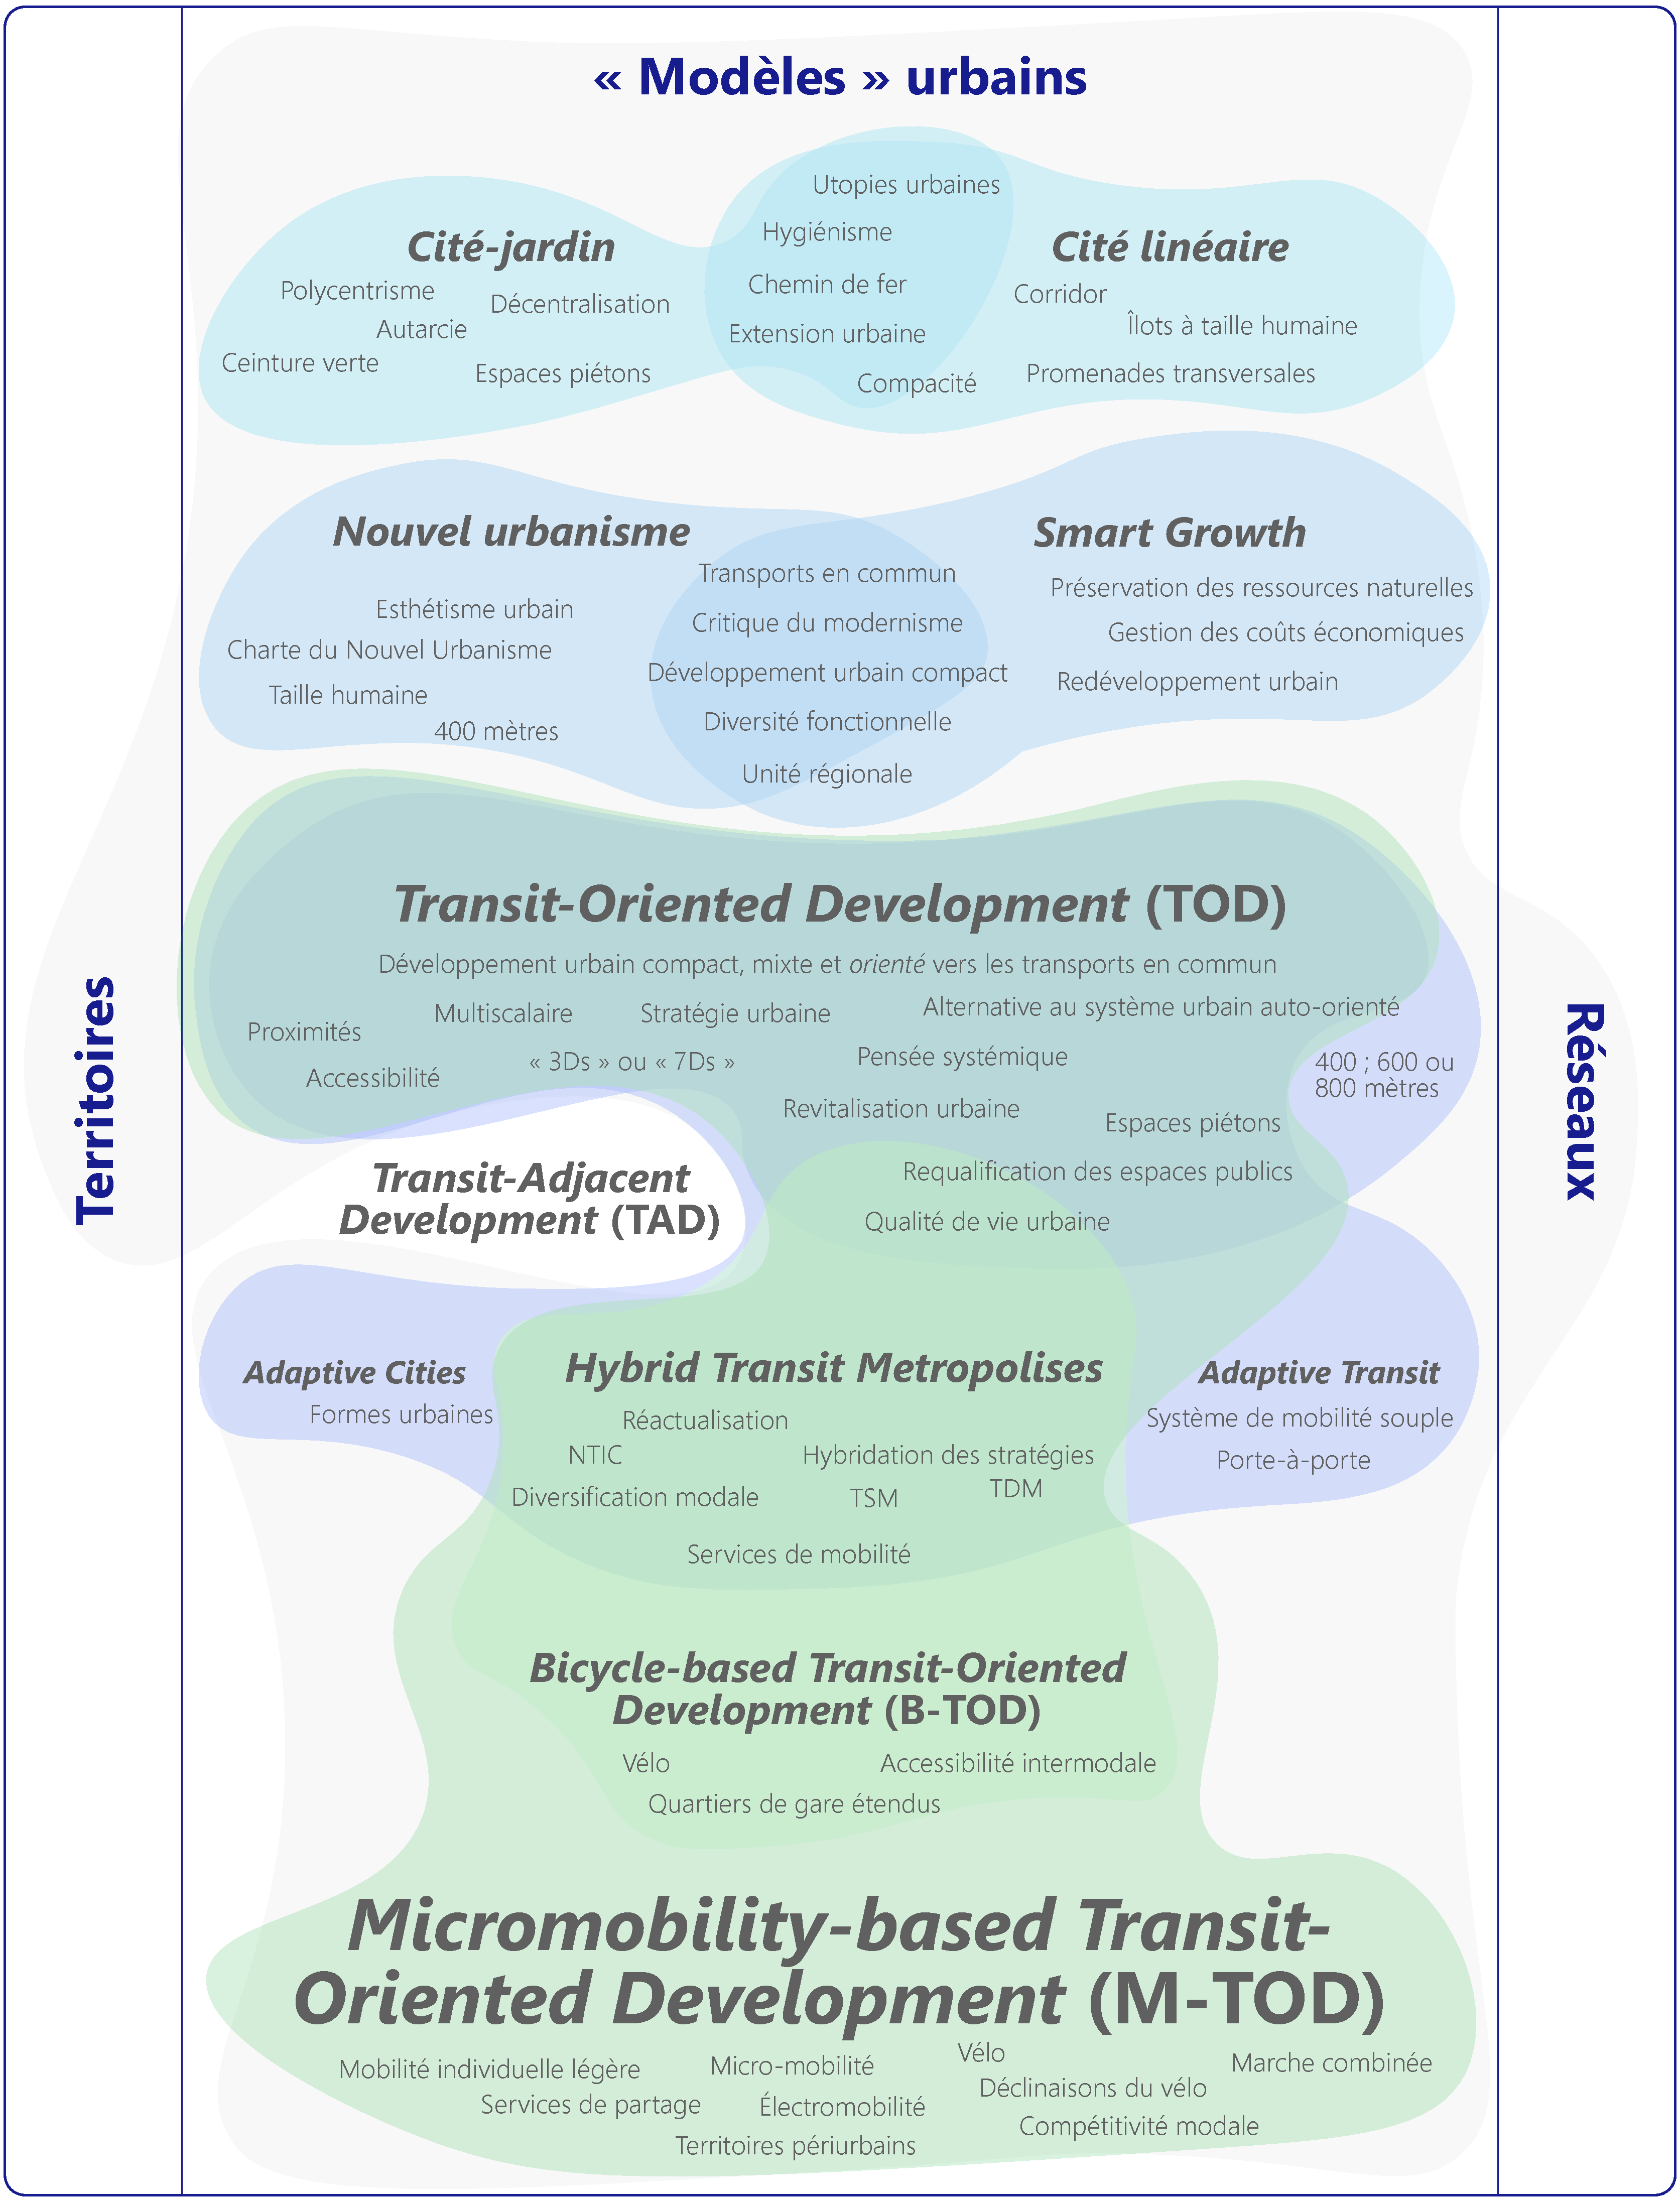
\includegraphics[width=1\columnwidth]{src/Figures/Graphical-abstract/FR_Graphical_abstract_chap1.pdf}}
        \vspace{5pt}
    \end{figure}
    
    % ___________________________________________
    % Préambule
    \newpage
    \begin{tcolorbox}[colback=white!5!white,
                      colframe=blue!75!blue,
                      title=
                      \bigskip
                      \center{\textbf{Préambule du chapitre~1}}
                      \\
                      \raggedright{\small{Chapitre composé de \pagedifference{chap1:titre}{chap2:titre} pages, dont \pagedifference{chap1:bibliographie}{chap2:titre} pages de bibliographie}}
                      \bigskip]
\Large{\textbf{\textcolor{blue}{Résumé~:}}}
    \\
    \small{
Formalisé aux États-Unis dans les années 1990, le \acrshort{TOD} constitue un modèle d'aménagement urbain reposant sur l’articulation entre densification, mixité fonctionnelle, requalification des espaces publics et développement du transport public, dans l’objectif de réduire la dépendance à l’automobile et de favoriser un système urbain plus résilient. Ce concept s’inscrit dans une filiation intellectuelle et urbanistique héritée de plusieurs courants historiques majeurs. Parmi eux, la \textsl{Cité-jardin} et la \textsl{Cité linéaire} ont introduit une planification structurée autour des infrastructures de transport en commun, tandis que le \textsl{Nouvel urbanisme} et la \textsl{Smart Growth} ont actualisé ces principes pour répondre aux défis de l’urbanisation contemporaine et de l’étalement urbain induit par la prééminence du modèle automobile. Le \textsl{TOD} se matérialise ainsi par une stratégie urbaine visant à structurer l’organisation territoriale \textsl{en connexion} avec le réseau de transport en commun, en promouvant une ville compacte, mixte et propice aux mobilités alternatives à l’automobile (voir la \hyperref[chap1:tod-presentation-generale]{section~1}, page~\pageref{chap1:tod-presentation-generale}).
    \\
Toutefois, la mise en œuvre du \acrshort{TOD} se heurte à plusieurs défis. Si ses principes demeurent particulièrement pertinents pour les métropoles bénéficiant d’un réseau de transport ferroviaire dense et performant, leur transposition aux territoires périurbains rencontre des obstacles structurels majeurs. L’allongement des distances de déplacement, la fragmentation des lieux et les limites intrinsèques des réseaux de transport en commun réduisent l’efficacité du modèle dans ces contextes. De plus, la rigidité des infrastructures lourdes complique leur adaptation aux formes urbaines héritées, caractérisées par un urbanisme peu dense et fortement auto-dépendant. Dans cette perspective, la montée en puissance de la mobilité individuelle légère~–~incluant le vélo, la trottinette et d’autres véhicules légers~–~offre un levier stratégique pour améliorer l’accessibilité aux stations de transport public et renforcer la connectivité des réseaux. Ce développement repose sur une diversité d’innovations techniques, servicielles et sociales, allant de l’électromobilité à la mutualisation des flottes en libre-service. Ainsi, l’intégration de ces modes pourrait permettre d’accroître la portée du \acrshort{TOD} et d’en maximiser les bénéfices (voir la \hyperref[chap1:mobilite-individuelle-legere]{section~2}, page~\pageref{chap1:mobilite-individuelle-legere}).
    \\
Ce chapitre explore, d’un point de vue théorique, le potentiel de la mobilité individuelle légère comme réponse aux limites du \textsl{Transit-Oriented Development} (\acrshort{TOD}). En facilitant les \Guillemets{premiers et derniers kilomètres}, cette famille de véhicules alternatifs optimise l’usage des infrastructures de transport en commun tout en réduisant la dépendance à l’automobile individuelle. Plutôt que de se substituer au transport public, elle s’inscrit dans une logique intermodale complémentaire, favorisant une intégration capillaire au sein des systèmes de mobilité. L’évolution des pratiques de déplacement et l’essor de ces (nouveaux) modes transforment ainsi la relation entre transport public et aménagement urbain, appelant à une relecture des modèles établis. C'est pourquoi nous proposons d’élargir le concept de \acrshort{TOD} vers un modèle urbain réactualisé, que nous désignons sous le terme de \acrshort{M-TOD}, en nous inspirant notamment des principes du \acrshort{B-TOD} (voir la \hyperref[chap1:btod]{section~3}, page~\pageref{chap1:btod}).
    }
    \tcblower
\Large{\textcolor{blue}{\textbf{Mots-clés~:}}}
    \\
    \small{
\textsl{Bicycle-based Transit-Oriented Development}~;
Électromobilité~;
Hybridation modale~;
\textsl{Hybrid Transit Metropolis}~;
Innovation~;
Mobilité individuelle légère~;
Mobilité partagée~;
\textsl{Transit-Oriented Development}
    }
    \end{tcolorbox}

    % ___________________________________________
    % 1.*.
    \newpage
    \needspace{1\baselineskip} % Réserve de l'espace
    \addcontentsline{toc}{section}{Introduction du chapitre~1}
    \sectionheader{Introduction du chapitre}
\section*{Introduction du chapitre~1
    \label{chap1:introduction}
    }
    \markright{Introduction du chapitre~1}{}

    % Citation
\begin{displayquote}
\Guillemets{\textsl{Le modèle} [du \textsl{Transit-Oriented Development}] \textsl{présenté dans cet ouvrage} [\dots] \textsl{se concentre sur les transports en commun et vise à élargir un mouvement plus vaste~–~l'Urbanisme Néo-Traditionnel et le Nouvel Urbanisme~–~qui englobe de nombreuses dimensions et diverses nuances. Bien que ces approches partagent des principes fondamentaux, elles s'orientent vers des voies sensiblement distinctes.} [\dots] \textsl{En ce qui concerne ces propositions, il est essentiel de garder à l'esprit qu'il n'y a pas de modèle absolu et que les particularités du lieu, tout comme les contextes économiques et politiques, auront toujours une influence sur les différentes orientations, en y créant un équilibre}}\footnote{
    \Guillemets{\textsl{The} [\textsl{Transit-Oriented Development}] \textsl{model presented in this book} [\dots] \textsl{focus on transit and is meant to broden a larger movement~–~Neo-Traditional Planning and the New Urbanism~–~which has many dimensions and differing emphasis. These approaches share fundamental principles but set out in slightly different directions.} [\dots] \textsl{With regards to all these proposals, it is important to remember that there is no absolute template and that the specifics of place, economics, and politics will always color and balance the different directions}} \textcolor{blue}{\autocite[10-11]{calthorpe_next_1993}}\index{Calthorpe, Peter|pagebf}.} [traduction libre]
    
\textcolor{blue}{Peter} \textcolor{blue}{\textcite[10-11]{calthorpe_next_1993}}\index{Calthorpe, Peter|pagebf}. \foreignlanguage{english}{\textsl{The Next American Metropolis: Ecology, Community, and the American Dream}}, Princeton Architectural Press, New York, 175~p. ISBN~: \href{https://search.worldcat.org/fr/title/27814585}{1-878271-68-7}
    \end{displayquote}

    % Introduction
\lettrine[lines=3, findent=8pt, nindent=0pt]{\lettrinefont F}{ace} aux enjeux de pollution, de fragmentation et de congestion urbaines engendrés par la diffusion massive de l’automobile et l’adaptation de l’urbanisation à ce mode de déplacement, le concept d’aménagement du \acrfull{TOD} repose sur le principe de densification et de diversification des activités et des usages autour des infrastructures de \gls{transport en commun}. Formalisé aux États-Unis sous l’impulsion de \textcolor{blue}{Peter} \textcolor{blue}{\textcite[10]{calthorpe_next_1993}}\index{Calthorpe, Peter|pagebf}, ce modèle urbain hérite de plusieurs courants de pensée, notamment de la \textsl{Cité-jardin} d’\textcolor{blue}{Ebenezer} \textcolor{blue}{\textcite{howard_-morrow_1898}}\index{Howard, Ebenezer|pagebf}, de la \textsl{Cité linéaire} d’\textcolor{blue}{Arturo Soria y Mata (1882)}, ainsi que des principes du \textsl{Nouvel urbanisme} et de la \textsl{Smart Growth}. Un élément fondamental du \acrshort{TOD} réside dans sa capacité à articuler explicitement transport public et aménagement urbain de manière synergique, bien au-delà d’une simple juxtaposition d’infrastructures et d’activités. Il s’agit d’une approche multidimensionnelle et multiscalaire où la station de transport en commun devient le pivot structurant du territoire. Dans cette logique, le point nodal ne se limite plus à \textsl{mettre} relation des flux, mais \textsl{entre} véritablement en interaction avec eux, en se connectant au lieu \textcolor{blue}{\autocite[344]{bertolini_nodes_1996}}\index{Bertolini, Luca|pagebf}, sur la base d'une approche de \Guillemets{lieu-mouvement} \textcolor{blue}{\autocite[103]{le_bot_flux_2024}}\index{Le Bot, Nils|pagebf}. Ce modèle vise ainsi à favoriser un urbanisme plus compact et animé, afin de mieux maîtriser l’étalement urbain et d’encourager les déplacements en transport en commun, mais aussi à pied et à \gls{vélo}. De plus, il contribue à la réorganisation des activités à l’échelle territoriale en favorisant une structure polycentrique \textcolor{blue}{\autocite[38]{pearce_enquete_2020}}\index{Pearce, Marc|pagebf}\index{Landriève, Sylvie|pagebf}\index{Gay, Christophe|pagebf}\index{Dubois, Tom|pagebf}, à l'allure d'une \Guillemets{décentralisation centralisée} \textcolor{blue}{\autocite[55]{kamruzzaman_advance_2014}}\index{Kamruzzaman, Md.|pagebf}\index{Baker, Douglas|pagebf}\index{Washington, Simon|pagebf}\index{Turrell, Gavin|pagebf}. Aujourd’hui, le \acrshort{TOD} s’affirme comme l'une des stratégies urbaines se rapprochant le plus à ce que nous pouvons qualifier d'\Guillemets{urbanisme durable} ou de \Guillemets{développement urbain \gls{durable}} \textcolor{blue}{\autocite[14]{bentayou_transit-oriented_2015}}\index{Bentayou, Gilles|pagebf}. Aussi, le dernier rapport du \acrfull{GIEC} préconise-t-il un développement urbain orienté vers les réseaux de transport en commun et les modes actifs, conçu pour favoriser une compacité urbaine \textcolor{blue}{\autocite[29]{lee_climate_2023}}\index{Lee, Hoesung|pagebf}\index{Calvin, Katherine|pagebf}\index{Dasgupta, Dipak|pagebf}\index{Krinner, Gerhard|pagebf}\index{Mukherji, Aditi|pagebf}\index{Thorne, Peter|pagebf}\index{Trisos, Christopher|pagebf}\index{Romero, Jose|pagebf}\index{Aldunce, Paulina|pagebf}\index{Barrett, Ko|pagebf}\index{Blanco, Gabriel|pagebf}\index{Cheung, William|pagebf}\index{Connors, Sarah|pagebf}\index{Denton, Fatima|pagebf}\index{Diongue Niang, Aïda|pagebf}\index{Dodman, David|pagebf}\index{Garschagen, Matthias|pagebf}\index{Geden, Oliver|pagebf}\index{Hayward, Bronwyn|pagebf}\index{|pagebf}\index{Jones, Christopher|pagebf}\index{Frank, Jotzo|pagebf}\index{Thelma, Krug|pagebf}\index{Laco, Rodel|pagebf}\index{Lee, June-Yi|pagebf}\index{Masson-Delmotte, Valérie|pagebf}\index{Meinshausen, Malte|pagebf}\index{Mintenbeck, Katja|pagebf}\index{Mokssit, Abdalah|pagebf}\index{Otto, Friederike~E.~L.|pagebf}\index{Pathak, Minal|pagebf}\index{Pirani, Anna|pagebf}\index{Poloczanska, Elvira|pagebf}\index{Pörtner, Hans-Otto|pagebf}\index{Revi, Aromar|pagebf}\index{Roberts, Debra~C.|pagebf}\index{Roy, Joyashree|pagebf}\index{Ruane, Alex~C.|pagebf}\index{Skea, Jim|pagebf}\index{Shukla, Priyadarshi~R.|pagebf}\index{Slade, Raphael|pagebf}\index{Slangen, Aimée|pagebf}\index{Sokona, Youba|pagebf}\index{Sörensson, Anna~A.|pagebf}\index{Tignor, Melinda|pagebf}\index{Vuuren, Detlef~van.|pagebf}\index{Wei, Yi-Ming|pagebf}\index{Winkler, Harald|pagebf}\index{Zhai, Panmao|pagebf}\index{Zommers, Zinta|pagebf}.%%Rédigé%%

    % Limites et intermodalité
Toutefois, l’allongement des distances et l'éclatement des lieux de production, de consommation et d’habitat, résultant du zonage fonctionnel et de l’artificialisation horizontale des sols, ont considérablement réduit l'attractivité et la compétitivité du transport public sur une grande partie des territoires \textcolor{blue}{\autocite[25-28]{mallet_voyage_2022}}\index{Mallet, Thierry|pagebf}. Par ailleurs, le système de transport en commun ne parvient pas à égaler l’ensemble des bénéfices procurés par l’automobilité, notamment en termes de flexibilité et de connectivité \textcolor{blue}{\autocite[209]{heran_retour_2015}}\index{Héran, Frédéric|pagebf}. Cette situation remet ainsi en question la capacité du modèle urbain à répondre efficacement à la dépendance automobile, en particulier dans les territoires périurbains. Une alternative réside dans la promotion de l’intermodalité, qui permettrait de pallier la rigidité du réseau de transport public \textcolor{blue}{\autocite[17]{wiel_comment_1998}}\index{Wiel, Marc|pagebf} et d’améliorer l’efficacité globale du système de mobilité \textcolor{blue}{\autocite[82]{oostendorp_combining_2018}}\index{Oostendorp, Rebekka|pagebf}\index{Gebhardt, Laura|pagebf}. En dépassant les approches strictement monoscalaires et monomodales, des mesures correctrices peuvent être mises en œuvre afin de limiter les dysfonctionnements et d’optimiser les performances des chaînes intermodales, de l’échelle régionale à l’échelle infra-urbaine \textcolor{blue}{\autocite[111-115]{chapelon_transports_2016}}\index{Chapelon, Laurent|pagebf}. Il s’agit ainsi de concevoir un système intégré et cohérent, où la croissance urbaine s’adapte au développement des transports en commun tout autant que les solutions de mobilité alternative s’ajustent aux spécificités du tissu urbain existant. Empiriquement, cette approche se traduit par l’adoption de stratégies urbanistiques favorisant un dialogue entre l’offre et la demande de transport, en intégrant des solutions de mobilité complémentaires au sein d’un système global et non plus sectorisé. C’est dans cette perspective que se sont développées les \textsl{Transit Metropolises} contemporaines, qui visent à concurrencer l’automobile en imitant sa connectivité \Guillemets{porte-à-porte} tout en s’inscrivant dans une logique de déplacement collectif \textcolor{blue}{\autocite[132-133]{cervero_transit_2020}}\index{Cervero, Robert|pagebf}.%%Rédigé%%

    % Mobilité individuelle légère
Dans ce contexte, la montée en puissance de ce que nous avons choisi d'appeler \Guillemets{mobilité individuelle légère}~–~comprenant le vélo, la trottinette et leurs diverses adaptations~–~ouvre de nouvelles perspectives en matière d’aménagement et de mobilité soutenables. Ces solutions offrent des alternatives intéressantes aux défis posés par les \Guillemets{premiers et derniers kilomètres} du transport public et s’imposent dès lors comme un chaînon manquant essentiel dans la transition vers une mobilité \Guillemets{écomobile} \textcolor{blue}{\autocites[4]{sebban_complementarite_2003}[25]{amar_homo_2016}{heran_transition_2018}}\index{Sebban, Annie-Claude|pagebf}\index{Motte, Alain|pagebf}\index{Héran, Frédéric|pagebf}\index{Amar, Georges|pagebf}. La mobilité individuelle légère s’inscrit dans une dynamique de \Guillemets{réécriture innovante du passé}, illustrée par le retour en force du vélo sous des formes renouvelées et par l’essor de la trottinette comme mode de déplacement utilitaire \textcolor{blue}{\autocite[18]{amar_homo_2016}}\index{Amar, Georges|pagebf}. Le développement de ces modes légers en tant que solutions intermodales témoigne d’un renouveau de la proximité à différentes échelles spatiales \textcolor{blue}{\autocite{sadik-kahn_15-minute_2021}}\index{Sadik-Kahn, Janette|pagebf}, renforçant ainsi l’attractivité du transport public et révélant une évolution des valeurs en matière de mobilité \textcolor{blue}{\autocite[110]{goletz_intermodality_2020}}\index{Goletz, Mirko|pagebf}\index{Haustein, Sonja|pagebf}\index{Wolking, Christina|pagebf}\index{L'Hostis, Alain|pagebf}. En fin de compte, la ville écomobile, en opposition au modèle de la ville automobile, repose sur une circulation de proximité où la complémentarité entre le vélo et le transport public constitue l’un des principes fondamentaux d’un système de mobilité plus intégré et résilient.%%Rédigé%%

    % Annonce du plan 1
Ce chapitre s’organise en trois grandes parties visant à explorer les fondements, l’application et l’évolution du \acrshort{TOD}. Dans un premier temps, nous examinerons les origines et les fondements théoriques de ce modèle urbain en retraçant ses influences historiques et intellectuelles, ainsi que son évolution et son applicabilité (\hyperref[chap1:tod-presentation-generale]{section~1}, page~\pageref{chap1:tod-presentation-generale}). Nous analyserons les courants d’urbanisme qui ont nourri son énonciation et sa codification avant de soulever les points d'originalité propres du \acrshort{TOD} (\hyperref[chap1:tod-presentation-generale-origines]{sous-section~1.1}, page~\pageref{chap1:tod-presentation-generale-origines}). Cette rétrospective épistémologique nous permettra d’en définir précisément les contours en tant que modèle de développement urbain alternatif au paradigme auto-centré, en précisant ses principes et les bénéfices attendus (\hyperref[chap1:tod-presentation-generale-definition]{sous-section~1.2}, page~\pageref{chap1:tod-presentation-generale-definition}). Enfin, nous verrons comment ce concept d'aménagement a été interprété au sein des stratégies urbaines déployées dans le contexte français et quelles sont ses principales déclinaisons en lien avec notre sujet de recherche (\hyperref[chap1:tod-presentation-generale-declinaisons]{sous-section~1.3}, page~\pageref{chap1:tod-presentation-generale-declinaisons}).%%Rédigé%%

    % Annonce du plan 2
La deuxième partie s’intéressera au second objet d’étude de cette recherche, à savoir la famille de véhicules regroupés sous l’appellation de \Guillemets{mobilité individuelle légère} (\hyperref[chap1:mobilite-individuelle-legere]{section~2}, page~\pageref{chap1:mobilite-individuelle-legere}). Nous retracerons l’évolution historique de ces objets techniques et sociaux~–~notamment le vélo et la trottinette~–~en identifiant et en simplifiant la lecture des grandes périodes qui ont marqué leur développement, dans le but de mieux contextualiser leur regain d’intérêt actuel (\hyperref[chap1:proximite-velo-trottinette]{sous-section~2.1}, page~\pageref{chap1:proximite-velo-trottinette}). Nous aborderons ensuite la diversification des usages et des formes de ces véhicules, qui se caractérise notamment par leur électrification et leur mise en partage dans l’\gls{espace public}, brouillant ainsi les frontières traditionnelles entre les modes de déplacement (\hyperref[chap1:velo-micromobilite-innovations]{sous-section~2.2}, page~\pageref{chap1:velo-micromobilite-innovations}). Cette réflexion historique nous permettra d’exposer à son tour l'évolution des valeurs attachées à la mobilité et aux modes de vie, ainsi que les enjeux de définition liés au périmètre de pertinence de cette famille de véhicules (\hyperref[chap1:caracterisation-mobilite-individuelle-legere]{sous-section~2.3}, page~\pageref{chap1:caracterisation-mobilite-individuelle-legere}).%%Rédigé%%

    % Annonce du plan 3
Enfin, la troisième partie du présent chapitre articulera les deux précédentes en explorant les opportunités qu’offre l’association entre transport public et mobilité individuelle légère dans une logique de complémentarité modale (\hyperref[chap1:btod]{section~3}, page~\pageref{chap1:btod}). Nous montrerons que, bien que la marche combinée ne soit pas assimilée à la mobilité individuelle légère, elle demeure l’élément structurant du \acrshort{TOD}. Dans un premier temps, nous démontrerons comment la portée réelle de la marche combinée tend à être sous-estimée et en quoi la mobilité individuelle légère peut jouer un rôle complémentaire, en s’inscrivant dans un champ de pertinence qui ne concurrence pas la marche, mais renforce l’\gls{accessibilité} au transport public (\hyperref[chap1:btod-limites-tod]{sous-section~3.1}, page~\pageref{chap1:btod-limites-tod}). Enfin, nous mettrons en évidence les avantages comparatifs d’une telle synergie et la manière dont cette approche intermodale nous invite à interroger la pertinence d’un modèle élargi, celui d'un \acrfull{M-TOD} (\hyperref[chap1:btod-m-tod]{sous-section~3.2}, page~\pageref{chap1:btod-m-tod}).%%Rédigé%%

     % ___________________________________________
    % 1.1.
    \newpage
    \needspace{1\baselineskip} % Réserve de l'espace
    \sectionheader{Concept d'aménagement du \textsl{Transit-Oriented Development}}
\section{Le \textsl{Transit-Oriented Development}, une réinvention de la planification régionale autour du chemin de fer
    \label{chap1:tod-presentation-generale}
    }

    % Introduction TOD
Le \acrshort{TOD} s’impose aujourd’hui comme un modèle d’aménagement clé dans la planification régionale, valorisant les infrastructures ferroviaires comme axe central de développement urbain. Cette stratégie popularisée repose sur l’idée de structurer les territoires autour des nœuds de transport public, dans le but de réduire la dépendance à la voiture individuelle et de promouvoir une urbanisation plus durable. En dépit de l’urgence et de l’importance de ces enjeux, les mécanismes sous-jacents influençant l’usage de la voiture en milieu urbain demeurent insuffisamment compris, en raison d’un cadre théorique encore limité \textcolor{blue}{\autocite[1]{verbavatz_critical_2019}}\index{Verbavatz, Vincent|pagebf}\index{Barthelemy, Marc|pagebf}. Les réflexions de l’architecte et urbaniste italien \textcolor{blue}{Alberto} \textcolor{blue}{\textcite[]{magnaghi_bioregion_2014}}\index{Magnaghi, Alberto|pagebf} apportent une contribution enrichissante à ce débat en introduisant une approche bioterritoriale, dans laquelle les \Guillemets{biorégions urbaines} et les réseaux deviennent les piliers d’un développement intégré et respectueux des écosystèmes locaux. Cependant, le \acrshort{TOD} figure parmi les rares concepts d’aménagement capables d’aborder et de traiter directement la pensée de l’\Guillemets{urbanisme des réseaux} \textcolor{blue}{\autocite[]{dupuy_urbanisme_1991}}\index{Dupuy, Gabriel|pagebf} dans un contexte globalisé, en mettant en lumière les interactions complexes entre mobilité, urbanisation et durabilité \textcolor{blue}{\autocite[51]{el_hadeuf_ville_2017}}\index{El Hadeuf, Mounya|pagebf}\index{Laterrasse, Jean|pagebf}.%%Rédigé%%

    % Annonce du plan
Nous commencerons par introduire, selon une approche diachronique, les origines du modèle urbain, en faisant ressortir les points sur lesquels il innove pour répondre aux enjeux contemporains liés à la nécessaire coordination entre réseau et territoire (\hyperref[chap1:tod-presentation-generale-origines]{section sur les inspirations du \textsl{Transit-Oriented Development}}, page~\pageref{chap1:tod-presentation-generale-origines}). Cette introduction sera suivie d’un état des lieux des principes généraux proposés par le modèle d’aménagement pour y remédier, ainsi que les effets attendus sur les territoires et les comportements de mobilité (\hyperref[chap1:tod-presentation-generale-definition]{section sur les directions du \textsl{Transit-Oriented Development}}, page~\pageref{chap1:tod-presentation-generale-definition}). Enfin, nous accorderons une attention particulière au caractère évolutif de ce concept à l’échelle mondiale, aussi bien dans les milieux académiques qu’opérationnels. Nous analyserons les diverses adaptations qui en découlent en fonction des spécificités de chaque terrain et de l'avancée des connaissances. Cette réflexion nous conduira à aborder le potentiel d’apport du vélo et de la \gls{micro-mobilité} dans une perspective de réactualisation du \acrshort{TOD} (\hyperref[chap1:tod-presentation-generale-declinaisons]{section sur les principales déclinaisons du \textsl{Transit-Oriented Development}}, page~\pageref{chap1:tod-presentation-generale-declinaisons}).%%Rédigé%%

    % 1.1.1. Chronologie TOD
    \needspace{1\baselineskip} % Réserve de l'espace
\subsection{Genèse du \textsl{Transit-Oriented Development}~: quand le rail inspire l'urbanisme
    \label{chap1:tod-presentation-generale-origines}
    }

    % Introduction 1
La géographie, tout comme de nombreuses disciplines connexes, a longtemps insisté sur l'interaction dynamique entre un lieu et son environnement, conceptualisant le lieu comme un \Guillemets{milieu} générateur d'activités et vecteur de transformations. En dépassant la simple notion d'espace physique, le système territorial agit à la fois comme \textsl{stimulus} et comme produit des transformations \textcolor{blue}{\autocite[19-21]{hagerstrand_what_1970}}\index{Hägerstrand, Torsten|pagebf}. Cette approche inclut la capacité des gares, en tant qu’espaces liminaux, à jouer un rôle de catalyseurs de développements variés \textcolor{blue}{\autocite[6]{baron_nouvelle_2024}}\index{Baron, Nacima|pagebf}\index{Le Bot, Nils|pagebf}\index{Detavernier, Pauline|pagebf}. Dans les années 1970, les \Guillemets{nouveaux géographes} ont ainsi orienté leurs travaux vers l’étude des réseaux \textcolor{blue}{\autocites{claval_nouveaux_1977}[166]{massardier_savants_1996}[112-113]{orain_geographie_2006}}\index{Massardier, Gilles|pagebf}\index{Claval, Paul|pagebf}\index{Orain, Olivier|pagebf}, en s’appuyant sur le maillage dense des infrastructures ferroviaires pour analyser les formes réticulaires. Ces recherches ont permis d’explorer les interactions réciproques entre réseau et territoire à différentes échelles géographiques \textcolor{blue}{\autocite[6]{baron_nouvelle_2024}}\index{Baron, Nacima|pagebf}\index{Le Bot, Nils|pagebf}\index{Detavernier, Pauline|pagebf}.%%Rédigé%%

    % Introduction 2
C’est dans ce contexte que l’architecte et urbaniste étasunien \textcolor{blue}{Peter} \textcolor{blue}{\textcite[10]{calthorpe_next_1993}}\index{Calthorpe, Peter|pagebf} propose un modèle d’aménagement centré sur le transport public, dans son ouvrage \foreignlanguage{english}{\textsl{The Next American Metropolis: Ecology, Community, and the American Dream}}~: le \acrfull{TOD}. Ce concept s’affirme comme une stratégie d'action multidimensionnelle, bien que majoritairement focalisée sur les aspects physico-spatiaux de l’aménagement \textcolor{blue}{\autocite[10]{calthorpe_next_1993}}\index{Calthorpe, Peter|pagebf}, en postulant que le changement de comportement de mobilité peut découler de la forme urbaine. Les influences majeures du \acrshort{TOD} s’inscrivent dans le cadre plus large du \textsl{Nouvel urbanisme} et de la \textsl{Smart Growth}, tout en apportant une nouvelle échelle d’analyse. En effet, \textcolor{blue}{Robert} \textcolor{blue}{\textcite[7]{cervero_transit_1998}}\index{Cervero, Robert|pagebf} considère que le \acrshort{TOD} déplace l’attention traditionnellement portée sur les interventions au niveau du quartier ou de la communauté vers les connexions entre les transports en commun et l’urbanisation sur le plan régional.%%Rédigé%%

    % 1.1.1.1. Mouvements d'urbanisme
    \needspace{1\baselineskip} % Réserve de l'espace
\subsubsection*{Héritage des réflexions urbanistiques passées
    \label{chap1:tod-presentation-generale-origines-mouvements}
    }

    % Introduction
Dans son ouvrage phare \textsl{L’urbanisme, utopies et réalités~: Une anthologie}, l’historienne \textcolor{blue}{Françoise} \textcolor{blue}{\textcite{choay_urbanisme_1965}}\index{Choay, Françoise|pagebf} offre une grille de lecture pour comprendre l’évolution des villes contemporaines. D'après la thèse défendue par l'autrice, la science de l'urbanisme telle que nous la connaissons aujourd'hui ne représente pas une solution novatrice à des problématiques nouvelles, mais réside essentiellement dans la réitération et la reproduction de schémas discursifs hérités du XIX\textsuperscript{e} siècle, qu'elle désigne comme des \Guillemets{modèles}. À cet égard, cette perspective permet d’interroger les fondements historiques et idéologiques du \acrshort{TOD}. Puisque le concept d'aménagement s'inscrit dans des courants de pensée, développés dans les années 1980 en réponse à la crise de l'urbanisation aux États-Unis, mais aussi en France \textcolor{blue}{\autocite[11]{lefebvre_droit_1967}}\index{Lefebvre, Henri|pagebf}, tels que le \textsl{New Urbanism} et la \textsl{Smart Growth}. Toutefois, réduire ses inspirations à ces mouvements post-modernes serait simpliste. Les racines de ce modèle s’étendent jusqu’aux théories urbanistiques de la fin du XIX\textsuperscript{e} siècle, notamment la \textsl{Cité-jardin}. \textcolor{blue}{Françoise} \textcolor{blue}{\textcite[259]{choay_urbanisme_1965}}\index{Choay, Françoise|pagebf} identifie cette dernière comme un \Guillemets{urbanisme culturaliste}, issu d'un courant théorique critique de la ville industrielle et caractérisé par une vision nostalgique d'un ordre organique\footnote{
    Dans sa typologie des mouvements de \Guillemets{pré-urbanisme} et d'\Guillemets{urbanisme}, \textcolor{blue}{Françoise} \textcolor{blue}{\textcite[277]{choay_urbanisme_1965}}\index{Choay, Françoise|pagebf} désigne comme \Guillemets{culturalistes} les courants théoriques datant de la seconde moitié du XIX\textsuperscript{e} siècle et qui prônent une ville circonscrite et fondée sur une organisation organique, en réaction aux idées progressistes de l'époque.
}.%%Rédigé%%

    % Cité-jardin : théorie
Le modèle du \acrshort{TOD} s’inspire largement du concept de la \textsl{Cité-jardin} (\textsl{Garden City}), développé à l’origine par l’urbaniste britannique \textcolor{blue}{Ebenezer} \textcolor{blue}{\textcite{howard_-morrow_1898}}\index{Howard, Ebenezer|pagebf}, en réaction à la croissance urbaine anarchique qui a accompagné l’industrialisation en Europe, caractérisée par une absence de planification urbaine. Sa pensée, formalisée dans son opuscule \textsl{Garden Cities of To-Morrow}, au caractère qualifié d’\Guillemets{urbaphobe} par certain·e·s observateur·rice·s \textcolor{blue}{\autocite[7]{cavin_cites-jardins_2007}}\index{Cavin, Joëlle Salomon|pagebf}, repose sur la création de villes satellites autosuffisantes, sur le \Guillemets{fantasme de la petite ville rêvée} \textcolor{blue}{\autocite[9]{fath_entre_2007}}\index{Fath, Sébastien|pagebf}, à échelle humaine, reliant les avantages de la vie urbaine et rurale. Ces villes sont conçues pour être limitées en taille et en extension, reliées par des réseaux ferroviaires, et organisées selon un système polycentrique, avec des ceintures vertes séparant chaque pôle urbain (voir le \hyperref[fig-chap1:schema-cite-jardin]{schéma~\ref{fig-chap1:schema-cite-jardin}}, page~\pageref{fig-chap1:schema-cite-jardin}). Ce projet social (\textsl{Social City}) vise à promouvoir une urbanité hybride tournée vers la nature, en opposition aux cités industrielles de son époque. Selon \textcolor{blue}{Robert} \textcolor{blue}{\textcite[38]{fishman_open_2011}}\index{Fishman, Robert|pagebf}, le \acrshort{TOD} emprunte aux cités-jardins les notions de décentralisation et de polycentrisme, mais également la conception d'espaces adaptés aux piéton·ne·s desservis par le chemin de fer.

    % Cité-jardin : exemples
Face au succès de la première cité-jardin, inaugurée à Letchworth en 1903 et conçue par \textcolor{blue}{Ebenezer Howard} \textcolor{blue}{\autocite[9]{gaboriau_aux_2004}}\index{Gaboriau, Arnaud|pagebf}, au nord de Londres, son importation en France est rapide, avec la construction de la première cité Bruno, à Dourges, dans le Pas-de-Calais, entre 1904 et 1908. Cette mise en œuvre des principes hygiénistes visait à loger les mineurs de la Compagnie des mines de Dourges. Il faut toutefois attendre l’entre-deux-guerres pour voir fleurir, autour des grandes villes françaises, un nombre important de cités-jardins. Les conceptions originelles y sont cependant réinterprétées. En effet, les cités-jardins à la française ne correspondent pas aux villes autonomes mettant en relation les lieux de travail, les commerces, les équipements collectifs et les logements qu’\textcolor{blue}{Ebenezer Howard} imaginait. Elles se présentent davantage comme des zones résidentielles, qualifiées de \Guillemets{banlieues-jardins}. Ce modèle subit ainsi une appropriation spécifique, qui écarte rapidement le volet économique fondé sur l’autosuffisance, tout en donnant lieu à de nombreuses réalisations se réclamant de ce concept \textcolor{blue}{\autocite[238]{guelton_cite-jardin_2013}}\index{Gaboriau, Arnaud|pagebf}. Un exemple emblématique de cette adaptation est celui des cités développées par la Compagnie des chemins de fer du Nord, sous l’impulsion de l’ingénieur \textcolor{blue}{Raoul Dautry}. À l'image de la cité de Lille-Délivrance, dont les travaux débutent en avril 1921, deux ans après l'édification d'une nouvelle gare de triage à Lomme et la mise en service d'une gare voyageur·se·s. Cette cité-jardin est directement adossée à la nouvelle gare. Lors de son inauguration en 1926, la cité de cheminots de Lille-Délivrance regroupe alors 835 logements et 3~228 habitant·e·s \textcolor{blue}{\autocite[19]{gaboriau_aux_2004}}\index{Gaboriau, Arnaud|pagebf}.%%Rédigé%%

   % Figure Cité-jardin
    \begin{carte}[h!]\vspace*{4pt}
        \caption{Schéma cartographique d'un réseau de six \Guillemets{cités-satellites} de 32~000 habitant·e·s entourant une \Guillemets{ville-centre} de 58~000 habitant·e·s.}
        \label{fig-chap1:schema-cite-jardin}
        \centerline{\includegraphics[width=0.75\columnwidth]{src/Figures/Chap-1/Cite_jardin.jpg}}
        \vspace{5pt}
        \begin{flushright}\scriptsize{
        Source~: \textcolor{blue}{Ebenezer} \textcolor{blue}{\textcite[90]{howard_-morrow_1898}}\index{Howard, Ebenezer|pagebf}, cité par \textcolor{blue}{Stephen} \textcolor{blue}{\textcite[3]{ward_garden_1992}}\index{Ward, Stephen|pagebf}
        }\end{flushright}
    \end{carte}

    % Cité linéaire : théorie
Un autre concept de cité utopique mise en application, dont s’inspire le \acrshort{TOD}, est sans nul doute la \textsl{Cité linéaire} (\textsl{Ciudad Lineal}), élaborée par \textcolor{blue}{Arturo Soria y Mata} en 1882 \textcolor{blue}{\autocite{lemelson_center_george_2014}}\index{Lemelson Center@\textsl{Lemelson Center}|pagebf}. En dirigeant le projet d’extension urbaine sur plus de cinq kilomètres le long de Madrid, l’urbaniste espagnol adopte une forme linéaire pour relier des centres urbains denses depuis les périphéries, une approche qui rappelle la notion de corridor chère au \acrshort{TOD} \textcolor{blue}{\autocite[348]{lopez_rodriguez_arturo_2017}}\index{López Rodríguez, Armando|pagebf}. L’organisation de la \textsl{Cité linéaire} repose sur un mode de transport en commun, souvent le tramway, qui devient la colonne vertébrale de l’agglomération \textcolor{blue}{\autocite{lemelson_center_george_2014}}\index{Lemelson Center@\textsl{Lemelson Center}|pagebf}. À la différence de la croissance urbaine traditionnelle, cette utopie urbaine envisage une ville sans banlieue, capable de contrôler son expansion le long d'un corridor \textcolor{blue}{\autocite[722]{furundzic_infrastructure_2012}}\index{Furundzic, Danilo~S.|pagebf}\index{Furundzic, Bozidar~S.|pagebf}. Par ailleurs, la \Guillemets{matrice de cette structure urbaine} se distingue par une accessibilité piétonne privilégiée, grâce à des promenades transversales reliant des îlots de densité moyenne. Ces deux utopies urbaines~–~la \textsl{Cité-jardin} et la \textsl{Cité linéaire}~–~prônent ainsi des questions qui sont toujours d'actualité et qui ont grandement influencé le \acrshort{TOD}, à savoir la promotion d'une ville compacte et conçue à la fois par et pour le transport public et la marche \textcolor{blue}{\autocite[11]{salomon_cavin_cites-jardins_2007}}\index{Salomon Cavin, Joëlle|pagebf}.%%Rédigé%%

    % Cité linéaire : exemples
L’expérimentation de cette cité idéale, initialement envisagée pour s’étendre sur 53 kilomètres autour de Madrid sous forme de boucle, ne verra finalement que 5 kilomètres réalisés, au nord-est de la capitale espagnole, à partir de 1894 \textcolor{blue}{\autocite[722]{furundzic_infrastructure_2012}}\index{Furundzic, Danilo~S.|pagebf}\index{Furundzic, Bozidar~S.|pagebf}. Ce projet, conçu par \textcolor{blue}{Arturo Soria y Mata}, prévoyait des connexions radioconcentriques reliant cette ceinture urbaine à la vieille ville. Inscrit dans le courant des villes hygiénistes, ce modèle exploite un axe ceinturant la ville existante pour faciliter la circulation des infrastructures essentielles telles que le chemin de fer, les réseaux de chauffage urbain, d’électricité ou encore de téléphonie. L’organisation horizontale de la ville linéaire rompt avec la structuration verticale propre à la ville bourgeoise, tout en anticipant certains principes de la cité-jardin, notamment l’accès généralisé à la propriété individuelle. Plus largement, ce concept évoque la notion de \Guillemets{Corridor Urbain} \textcolor{blue}{\autocite[63]{liu_corridors_2016}}\index{Liu, Liu|pagebf}\index{Menerault, Philippe|pagebf}\index{L'Hostis, Alain|pagebf}, en permettant d’étendre les villes de manière linéaire. À cet égard, des projets urbains tels que le \Guillemets{Grand Boulevard} reliant Lille, Roubaix et Tourcoing peuvent être considérés comme en résonance avec ces principes. Inaugurée en 1909, cette artère stratégique, longue de 14 kilomètres et large de 50 mètres, est traversée par six espaces de circulation dédiés respectivement à l'automobile, au transport lourd à cheval, au tramway Mongy, aux cavalier·ère·s, aux cyclistes et aux marcheur·se·s qui bénéficient de larges promenades\footnote{
        Aujourd’hui, le Grand Boulevard est néanmoins perçu comme un espace davantage assimilé à un lieu de transit automobile \textcolor{blue}{\autocite[139]{maitre_ambivalence_2016}}\index{Maitre, Elisa|pagebf}. Conçu initialement comme une artère urbaine intégrant deux chaussées séparées, des pistes cyclables et des trottoirs, cet aménagement a progressivement évolué pour devenir une voie rapide urbaine, au gré des raccordements successifs qui ont accru le trafic qu’il supporte. \textcolor{blue}{Philippe} \textcolor{blue}{\textcite[155]{menerault_gares_2008}}\index{Menerault, Philippe|pagebf} donne l'exemple de son intégration à l'autoroute A1, dont la première section jusqu'à Carvin est mise en service en 1954, et à l'autoroute A25, en direction de Dunkerque, en 1972.
} \textcolor{blue}{\autocite[87]{demangeon_lille-roubaix-tourcoing_1988}}\index{Demangeon, Alain|pagebf}\index{Werquin, Ann-Carol|pagebf}. Pensé comme un outil structurant de la croissance urbaine, ce projet avait pour ambition de faire du Grand Boulevard une vitrine régionale, surnommée les \Guillemets{Champs-Élysées} de la métropole, et d’en faire la colonne vertébrale de la future métropole \textcolor{blue}{\autocite{dubuis__2020}}\index{Dubuis, Angélique Da Silva|pagebf}. La ville linéaire a par ailleurs suscité d’autres interprétations et prolongements, notamment dans les expériences soviétiques ou à travers la reprise de ce concept par \textcolor{blue}{Le Corbusier}. Plus récemment, un exemple marquant est le projet \textsl{The Line}, annoncé par les autorités saoudiennes dans le cadre du plan Vision 2030 \textcolor{blue}{\autocite[139]{arnault_ville_2022}}\index{Arnault, Julie|pagebf}. Inscrit dans le projet de ville nouvelle \textsl{Neom}, ce concept, actuellement en cours de réalisation, repose sur la création d’une ville linéaire de 170 kilomètres de long pour 200 mètres de large et 500 mètres de hauteur\footnote{
    Cependant, avant même son lancement concret, le projet \textsl{The Line} est revu à la baisse pour 2030, avec une infrastructure longue de seulement 2,4 kilomètres au lieu des 170 kilomètres initialement prévus.
}. Cette infrastructure sera desservie par un train à grande vitesse, permettant théoriquement de parcourir l’ensemble de la ville en moins de 20 minutes. Les services essentiels seront répartis en hauteur, à chaque étage, et accessibles en moins de cinq minutes \textcolor{blue}{\autocite[139]{arnault_ville_2022}}\index{Arnault, Julie|pagebf}.%%Rédigé%%

    % New Urbanism
Sous un regard plus contemporain, l’enracinement du \acrshort{TOD} trouve une origine directe dans le \textsl{Nouvel urbanisme} (\textsl{New Urbanism}), un courant urbanistique et architectural apparu dans les années 1980 en réponse aux limites de l’urbanisme moderne \textcolor{blue}{\autocite[71]{liu_analyse_2016}}\index{Liu, Liu|pagebf}. Ce mouvement critique notamment le manque de diversité fonctionnelle et architecturale, l’organisation inadéquate des espaces publics et l’insuffisance de place accordée aux piéton·ne·s. Proposé comme une alternative rationnelle au développement des quartiers résidentiels pavillonnaires à faible densité et largement dominés par l’automobile, le \textsl{Nouvel urbanisme} ambitionne de repenser l’aménagement urbain pour le rendre plus humain, esthétique et fonctionnel. Bien qu’inspiré par certains principes du mouvement moderne, il s’en démarque notamment par l’instauration, en 1989, du \textsl{Congress for the New Urbanism}, souvent perçu comme l’équivalent contemporain du \acrfull{CIAM}. En 1996, ce Congrès ratifie sa propre Charte du Nouvel Urbanisme (\textsl{Charter of the New Urbanism})\footnote{
    Ce mouvement ne constitue toutefois pas un bloc monolithique. Il se compose de deux grandes approches complémentaires \textcolor{blue}{\autocite[178]{ouellet_smart_2006}}\index{Ouellet, Michel|pagebf}. D’une part, les partisan·e·s du \acrfull{TND} qui mettent l’accent sur une esthétique et une organisation urbaine néotraditionnelle, favorisant des quartiers compacts avec un habitat aligné le long de rues à intersections multiples. D’autre part, les promoteur·rice·s du \acrshort{TOD} qui privilégient l’intégration du transport public et une planification urbaine régionale plus respectueuse de l’environnement. Bien que distinctes, ces deux visions partagent un objectif commun~: encourager des formes urbaines favorisant la mixité fonctionnelle et la réduction de l’empreinte écologique des territoires.
}. Cette \Guillemets{philosophie d’aménagement} met en avant un développement urbain compact, planifié à l’échelle humaine, qui privilégie les transports en commun et l’intégration de fonctions urbaines diverses \textcolor{blue}{\autocite[177]{ouellet_smart_2006}}\index{Ouellet, Michel|pagebf}. D'un point de vue pratique, elle reconnaît plusieurs caractéristiques principales au quartier, dont celle de sa dimension optimale, évaluée à 400 mètres du centre à la périphérie \textcolor{blue}{\autocite[194]{ducharme_ville_2021}}\index{Ducharme, Olivier|pagebf}. Enfin, le \textsl{Nouvel urbanisme} adopte une perspective régionale, considérant la région comme unité territoriale de base dans un contexte de mondialisation économique \textcolor{blue}{\autocite[]{calthorpe_regional_2001}}\index{Calthorpe, Peter|pagebf}\index{Fulton, William|pagebf}. Dans cette perspective, le \acrshort{TOD} hérite l’objectif de promouvoir les transports en commun dans le but de freiner l'artificialisation des sols non urbanisés \textcolor{blue}{\autocite[117]{lo_feudo_scenario_2014}}\index{Lo Feudo, Fausto|pagebf}\index{Menerault, Philippe|pagebf}\index{L'Hostis, Alain|pagebf}\index{Festa, Demetrio Carmine|pagebf}.%%Rédigé%%

    % Smart Growth
Les principes du \acrshort{TOD} trouvent également leurs racines dans un courant majeur de l’urbanisme contemporain~: la \textsl{Smart Growth}, qui émerge à la fin des années 1980 et qui se structure au milieu des années 1990 dans le prolongement du paradigme du \Guillemets{développement urbain durable} \textcolor{blue}{\autocites[7]{bentayou_transit-oriented_2015}[71]{liu_analyse_2016}}\index{Bentayou, Gilles|pagebf}\index{Liu, Liu|pagebf}. Ce mouvement vise à préserver les ressources naturelles et financières, tout en cherchant à réduire les ségrégations spatiales, qu’elles soient fonctionnelles ou sociales \textcolor{blue}{\autocite[7]{bentayou_transit-oriented_2015}}\index{Bentayou, Gilles|pagebf}. La \textsl{Smart Growth} s’oppose explicitement à l’étalement urbain non maîtrisé, en promouvant des formes d’aménagement plus compactes et le redéveloppement urbain \textcolor{blue}{\autocites[176]{ouellet_smart_2006}{smart_growth_network_what_2015}}\index{Ouellet, Michel|pagebf}\index{Smart Growth Network@\textsl{Smart Growth Network}|pagebf}. Ces principes, partagés par le \textsl{Nouvel urbanisme}, valorisent une approche intégrée, où transport et urbanisme convergent pour créer des environnements durables, socialement équitables et économiquement viables. Le \acrshort{TOD} serait ainsi l'un des outils permettant de faire advenir ce \Guillemets{nouvel} urbanisme \Guillemets{intelligent} \textcolor{blue}{\autocite[7]{bentayou_transit-oriented_2015}}\index{Bentayou, Gilles|pagebf}.%%Rédigé%%

    % Figure photographies Val d'Europe
    \begin{figure}[h!]\vspace*{4pt}
        \caption{Photographies du secteur Val d'Europe, le 13 septembre 2023.}
        \label{fig-chap1:photographies-val-europe}
        \centerline{\includegraphics[width=0.75\columnwidth]{src/Figures/Chap-1/Val_Europe.jpg}}
        \vspace{5pt}
        \begin{flushright}\scriptsize{
        Photographies (A), (B), (C) et (D)~: \textcolor{blue}{Dylan Moinse (2023)}
      }\end{flushright}
    \end{figure}
    
    % Exemples New Urbanism/Smart Growth
Des réalisations emblématiques illustrent les principes du \textsl{Nouvel Urbanisme} et de la \textsl{Smart Growth}, à l'instar du quartier résidentiel de Laguna West, à Sacramento, en Californie, développé par \textcolor{blue}{Peter} \textcolor{blue}{\textcite[146-149]{calthorpe_next_1993}}\index{Calthorpe, Peter|pagebf}, figure clé de ces mouvements. Il s'agit d'une \Guillemets{communauté} néotraditionnelle, dont le projet lancé en 1989 intègre 3~400 unités résidentielles, en s'appuyant sur les concepts pionniers de l'architecte et urbaniste étasunien \textcolor{blue}{Morris} \textcolor{blue}{\textcite[]{newman_focus_1991-1}}\index{Newman, Morris|pagebf}. Aussi, tournons-nous vers l'étude du projet urbain Val d'Europe, le quatrième secteur de la ville nouvelle de Marne-la-Vallée, primé par le \textsl{Prix de la Charte} (\textsl{Charter Awards}) en 2006, par le \textcolor{blue}{\textcite{congress_for_the_new_urbanism_cnu_2006}}\index{Congress for the New Urbanism@\textsl{Congress for the New Urbanism}|pagebf}. Ce projet urbain, développé le long de la ligne A du \acrfull{RER} francilien~–~ligne la plus fréquentée d'Europe et mise en service en 1969, bien que la station Val d'Europe soit inaugurée en 2001~–~bénéficie d'une localisation stratégique à proximité immédiate de la gare \acrshort{TGV} de Marne-la-Vallée~–~Chessy. Il s'agit d'un \acrfull{PPP} né d'une collaboration entre l'État français et la \Marque{Walt Disney Company}, scellée par un accord en 1987, visant à développer et à exploiter \Marque{Euro Disneyland}, tout en intégrant un centre urbain dans la ville nouvelle \textcolor{blue}{\autocite{epamarne_val_nodate}}\footnote{
    L'\acrfull{EPA} ÉpaMarne, en collaboration avec ÉpaFrance a été chargé du pilotage de Val d'Europe dans le cadre d'une stratégie visant à équilibrer le développement territorial de la région Île-de-France, traditionnellement polarisée par l'attractivité du \acrfull{CBD} de La Défense. Ce projet incarne une double ambition~: d'une part, la création d'un centre urbain autonome en périphérie immédiate de Paris et, d'autre part, le renforcement de l'attractivité touristique régionale grâce à l'implantation de Disneyland Paris.
}. La planification de Val d'Europe repose sur trois principes fidèles aux mouvements présentés plus tôt~: (i) une organisation en quartiers, places et rues, favorisant des échelles humaines~; (ii) une mixité sociale fonctionnelle, intégrant logements\footnote{
    À l'heure actuelle, le développement urbain de Val d'Europe se poursuit. Adopté en 2016, le premier \acrfull{PLUi} de l'\acrshort{EPCI} prévoit la construction de 650 logements par an, visant un total de 5~100 unités, dont 80~\% de logements familiaux. Ce plan vise également à s'adapter aux exigences de la \acrfull{SRU} en matière de parc social, en prévoyant 34~\% de logements sociaux parmi les logements à venir, d'après son \acrfull{PLH}.
}, commerces et services\footnote{
    Prenons pour exemple le centre commercial Val d'Europe, ouvert en 2000, qui constitue le cœur symbolique et fonctionnel de la ville. Celui-ci est divisé en zones thématiques et a été récompensé pour son \textsl{design} (\textsl{International Council of Shopping Centers Europe awards}).
}~; et (iii) une architecture inspirée de l'histoire européenne, conférant une identité à chacun des quartiers (voir l'\hyperref[fig-chap1:photographies-val-europe]{illustration~\ref{fig-chap1:photographies-val-europe}}, page~\pageref{fig-chap1:photographies-val-europe}). Ainsi que l'exposent \textcolor{blue}{\textcite[25]{dupuis_nouvelle_2017}}\index{Dupuis, Blaise|pagebf}\index{Söderström, Ola|pagebf}, en tant que \Guillemets{nouvelle ville traditionnelle}, Val d'Europe porte haut les principes prônés\footnote{
    Toutefois, le développement de Val d'Europe suscite des interrogations quant à son modèle de gouvernance et sa conception urbaine. L'implication de l'opérateur privé dans la gestion urbaine a imposé une vision entrepreneuriale, voire commerciale, de la fabrique urbaine. Cette approche a souvent été critiquée pour sa tendance à une \Guillemets{disneylandisation} ou une \Guillemets{muséification} de l'espace urbain \textcolor{blue}{\autocite[]{brunel_planete_2012}}\index{Brunel, Sylvie|pagebf}. Ces notions renvoient à un modèle idéalisé et hyper-contrôlé, caractérisé par une reproduction fictive et standardisée de paysages et d'histoires urbaines, destinés à répondre aux attentes stéréotypées des touristes \textcolor{blue}{\autocite[7]{claude_developpement_2021}}\index{Claude, Appolline|pagebf}\index{Laage de Meux, Olivia de|pagebf}\index{Delpuech, Inès|pagebf}\index{Dextreit, Natalia|pagebf}\index{Poquillon, Mathilde|pagebf}\index{Praderie, Mila|pagebf}. Les critiques soulignent également les risques d'une déconnexion entre cette ville idéalisée et les réalités sociales et économiques. Elles questionnent notamment l'équilibre entre les impératifs entrepreneuriaux, l'inclusion sociale et la durabilité. En outre, les processus de négociation entre acteurs publics et privés ont été marqués par des tensions, révélant les limites d'un \acrshort{PPP} dans ces types de projet urbain. Un exemple est celui de la localisation du centre commercial régional Val d'Europe. L'opérateur privé, probablement affecté par une \Guillemets{culture de l'indifférence vis-à-vis du transport public} \textcolor{blue}{\autocite[656]{tan_identifying_2014}}\index{Tan, Wendy|pagebf}\index{Bertolini, Luca|pagebf}\index{Janssen-Jansen, Leonie|pagebf}, souhaitait implanter cet équipement en bordure d'autoroute, loin du pôle d'échange et de la station \acrshort{RER}.
}, à savoir une compacité urbaine, une organisation en quartiers, ainsi que des principes esthétiques et morphologiques ancrés dans l'héritage des siècles passés \textcolor{blue}{\autocite[12]{moinse_exploring_2023}}\index{Moinse, Dylan|pagebf}.%%Rédigé%%

    % Transition
Le concept d’aménagement du \acrshort{TOD}, centré sur un développement urbain compact, mixte et structuré autour d’un nœud de transport, s’inscrit dans une lignée de mouvements urbanistiques qui l’ont précédé. Ces influences sont pleinement revendiquées par \textcolor{blue}{Peter Calthorpe}, l’un des principaux théoriciens du \acrshort{TOD}, qui se définit comme \Guillemets{un restaurateur et non un initiateur d’idées}\footnote{
    \Guillemets{\textsl{Mr. Calthorpe, who calls himself a reviver rather than an originator of ideas} [\dots]} \textcolor{blue}{\autocite[5]{newman_focus_1991}}\index{Newman, Morris|pagebf}.
} \textcolor{blue}{\autocite[5]{newman_focus_1991}}\index{Newman, Morris|pagebf}. Si des prémices du \acrshort{TOD} peuvent être identifiées dans des modèles tels que la \textsl{Cité-jardin} ou la \textsl{Cité linéaire}, ou encore de grandes figures de l'histoire de l'urbanisme comme \textcolor{blue}{Ildefons Cerdà} ou \textcolor{blue}{Georges-Eugène Haussmann}, ces exemples témoignent de l’évolution des idées en matière d’aménagement urbain. Dans la cité-jardin, par exemple, la gare joue un rôle fonctionnel limité, se réduisant à relier des cités autosuffisantes entre elles et à leur environnement. \textcolor{blue}{Peter} \textcolor{blue}{\textcite[43-49]{calthorpe_next_1993}}\index{Calthorpe, Peter|pagebf}, en revanche, renverse ce principe~: dans le \acrshort{TOD}, la station de transport devient le centre structurant de l’aménagement urbain, dépassant la logique d’autarcie pour créer du lien au sein d’une ville contemporaine fragmentée et dispersée \textcolor{blue}{\autocite[51]{el_hadeuf_ville_2017}}\index{El Hadeuf, Mounya|pagebf}\index{Laterrasse, Jean|pagebf}. Cette distinction marque un tournant conceptuel. Contrairement au \textsl{Nouvel urbanisme} et à la \textsl{Smart Growth}, qui s’opposent principalement à l’étalement urbain non maîtrisé, le \acrshort{TOD} affirme un rôle moteur pour les infrastructures de transport dans la structuration de la ville \textcolor{blue}{\autocite[51]{el_hadeuf_ville_2017}}\index{El Hadeuf, Mounya|pagebf}\index{Laterrasse, Jean|pagebf}. Là où le \textsl{Nouvel urbanisme} promeut une densité humaine et esthétique, et où la \textsl{Smart Growth} privilégie la préservation des ressources naturelles et la mixité fonctionnelle, le \acrshort{TOD} se distingue par son ambition de reconnecter les territoires épars grâce à une organisation centrée sur le transport. Bien que la plupart des composantes morphologiques~–~présence d'une gare, densité et compacité~–~soient semblables, cette approche traduit un changement d’échelle entre la ville du XIX\textsuperscript{e} siècle, encore pensée comme un tout cohérent, et la ville contemporaine, qui nécessite des outils pour rétablir sa cohésion \textcolor{blue}{\autocite[37]{leysens_reconfiguration_2011}}\index{Leysens, Thomas|pagebf}\index{Menerault, Philippe|pagebf}\index{L'Hostis, Alain|pagebf}.%%Rédigé%%

    % 1.1.1.2. TOD aspects contemporains
    \needspace{1\baselineskip} % Réserve de l'espace
\subsubsection*{Originalité et réinterprétation de la planification autour du rail
    \label{chap1:tod-presentation-generale-origines-originalite}
    }

    % Introduction
Le mouvement ayant vu naître le \acrshort{TOD} s'inscrit dans une filiation intellectuelle et urbanistique commune à plusieurs courants critiques et militants, unis par leur opposition au paradigme de la ville auto-centrée\footnote{
    Dès les années 1960, et même dès l'après-guerre, la domination de l’automobile dans l’espace urbain commence à être remise en question, suscitant des critiques croissantes concernant son usage massif et ses implications pour l’aménagement urbain \textcolor{blue}{\autocites{jacobs_death_1961}{illich_energie_1973}}\index{Jacobs, Jane|pagebf}\index{Illich, Ivan|pagebf}\index{Giard, Luce|pagebf}\index{Bardet, Vincent|pagebf}. Ce passage au \Guillemets{troisième âge de la ville} \textcolor{blue}{\autocite[4]{newman_land_1996}}\index{Newman, Peter W.~G.|pagebf}\index{Kenworthy, Jeffrey~R.|pagebf} marqué par la \Guillemets{culture de l'automobile} \textcolor{blue}{\autocite[157]{urry_social_2003}}\index{Urry, John|pagebf}. structure encore aujourd'hui la plupart des territoires, avec des conséquences directes et indirectes sur l'aménagement, les comportements de mobilité et les modes de vie \textcolor{blue}{\autocite[40]{sebban_complementarite_2003}}\index{Sebban, Annie-Claude|pagebf}\index{Motte, Alain|pagebf}.
} \textcolor{blue}{\autocites{jacobs_death_1961}{illich_energie_1973}}\index{Jacobs, Jane|pagebf}\index{Illich, Ivan|pagebf}\index{Giard, Luce|pagebf}\index{Bardet, Vincent|pagebf}, et notamment les nombreuses externalités négatives associées à ce modèle\footnote{
    Les externalités négatives engendrées par la dépendance à l’automobile incluent des nuisances internes telles que la congestion urbaine, qui compromet l’attractivité économique et résidentielle des territoires, mais également des effets externes plus larges~: accidents de la route, effets de \gls{coupure urbaine}, sédentarisation, fragmentation de l’espace, exclusion socio-spatiale, consommation accrue d’espaces agricoles et naturels, perte de biodiversité, pollutions multiples (air, eau, sols, sonore et visuelle), ainsi qu’une dégradation de la qualité de vie, allant de problèmes de santé physique et mentale à un stress chronique et à une réduction de la productivité. Ces externalités contribuent à ce que certain·e·s auteur·rice·s qualifient de \Guillemets{spirale de la dépendance à l’automobile} ou \Guillemets{cycle de l’auto-dépendance}, dans lequel l’automobile crée des problèmes que seul son usage intensifié semble pouvoir résoudre \textcolor{blue}{\autocites[62]{cervero_transit_1998}[4]{heran_reduction_2001}[2]{heran_zones_2009}}\index{Cervero, Robert|pagebf}\index{Héran, Frédéric|pagebf}\index{Pouillaude, Laurence|pagebf}.
} \textcolor{blue}{\autocites[62]{cervero_transit_1998}[4]{heran_reduction_2001}[2]{heran_zones_2009}}\index{Cervero, Robert|pagebf}\index{Héran, Frédéric|pagebf}\index{Pouillaude, Laurence|pagebf}. Le \Guillemets{système automobile}, caractérisé par un mode d’organisation centré sur les performances techniques et les avantages apparents de la voiture, constitue une structure captative et rigide\footnote{
    La dépendance à l’automobile, ainsi que l'\Guillemets{automobilité} désignant un mode de vie et les représentations associées, reposent sur des facteurs culturalistes, socio-économiques, urbanistiques et technicistes \textcolor{blue}{\autocite[12]{heran_reduction_2001}}\index{Héran, Frédéric|pagebf}. Le \Guillemets{tout-automobile} est le produit d'aspirations liées à la propriété individuelle d'une maison et d'un jardin, d'une élévation des niveaux de vie conjuguée à des normes de consommation, de l'influence de formes urbaines favorisant les déplacements motorisés et de l'amélioration continue des performances de la voiture par rapport aux autres modes de déplacement.
}. Les \Guillemets{coûts cachés} associés à ce système, c'est-à-dire les coûts non couverts par la collectivité qui sont estimés à environ 3~\% du \acrfull{PIB} annuel de l'\acrfull{UE}, révèlent son inefficacité collective \textcolor{blue}{\autocite[34]{becker_couts_2012}}\index{Becker, Udo~J.|pagebf}\index{Becker, Thilo|pagebf}\index{Gerlach, Julia|pagebf} et sa contribution à une véritable \Guillemets{tragédie des communs} \textcolor{blue}{\autocite{hardin_tragecommuns_1968}}\index{Hardin, Garrett|pagebf}, où l’usage intensif des espaces routiers par certains individus entraîne des conséquences délétères pour l’ensemble de la société \textcolor{blue}{\autocite[23]{6t-bureau_de_recherche_livre_2019}}\index{Bureau de recherche 6t@\textsl{Bureau de recherche 6t}|pagebf}. À noter que ces estimations restent, de surcroît, sous-évaluées, notamment en raison de la non-prise en compte systématique des boucles de rétroaction complexes affectant le dérèglement climatique et la santé publique \textcolor{blue}{\autocite[66, 72]{gossling_social_2019}}\index{Gössling, Stephan|pagebf}\index{Choi, Andy|pagebf}\index{Dekker, Kaely|pagebf}\index{Metzler, Daniel|pagebf}. C’est précisément dans ce contexte critique que le concept du \acrshort{TOD} se déploie, comme une réponse multidimensionnelle visant à remédier aux dysfonctionnements du modèle auto-centré.%%Rédigé%%

    % Lutte contre la dépendance automobile
En effet, plus qu’une invention \textsl{ex nihilo}, le \acrshort{TOD} constitue avant tout le résultat d’une adaptation à un contexte urbain renouvelé, celui de la complexité et de la \Guillemets{vitesse} des villes modernes. Il propose une alternative articulée à la diffusion et à l'usage généralisés de l'automobile en introduisant des principes, des perspectives et des outils opérationnels pour répondre aux enjeux actuels, à différentes échelles spatiales \textcolor{blue}{\autocite[37]{leysens_reconfiguration_2011}}\index{Leysens, Thomas|pagebf}. C'est là que se trouvent les apports originaux du modèle \textcolor{blue}{\autocite[121]{lo_feudo_scenario_2014}}\index{Lo Feudo, Fausto|pagebf}\index{Menerault, Philippe|pagebf}\index{L'Hostis, Alain|pagebf}\index{Festa, Demetrio Carmine|pagebf}~: il faut abandonner l'idée que l'automobile est l'étalon de mesure servant à la planification de l'espace urbain \textcolor{blue}{\autocite[190]{ducharme_ville_2021}}\index{Ducharme, Olivier|pagebf}. \textcolor{blue}{Peter} \textcolor{blue}{\textcite{calthorpe_next_1993}}\index{Calthorpe, Peter|pagebf} a ainsi essentiellement formalisé la relation étroite entre développement urbain et transports en commun, érigée en principe structurant du \acrshort{TOD}. Ce dernier définit dans ce cadre les bases d’un \Guillemets{nouveau rêve américain} (\textsl{American Dream})~: contrairement aux courants précurseurs principalement axés sur des préoccupations esthétiques ou sociales, le \acrshort{TOD} privilégie une approche résolument régionale. Il ne s'agit plus seulement d'une somme de projets urbains dispersés et éparpillés dans une ville contemporaine \textcolor{blue}{\autocite[357]{mongin_ville_2013}}\index{Mongin, Olivier|pagebf}. Il intègre l’impératif de réduction de l’usage de l’automobile au cœur même des fonctions de l’urbanisme \textcolor{blue}{\autocite[11]{calthorpe_next_1993}}\index{Calthorpe, Peter|pagebf}.%%Rédigé%%

    % Oriented
C'est là la seconde innovation apportée par le \acrshort{TOD}, qui réside dans sa faculté à s’ajuster au contexte de croissance de l’usage de l’automobile, tout en proposant une réflexion collective nourrie d’expériences internationales. Il introduit notamment un troisième élément structurant dans la relation entre \textsl{transit} et \textsl{development}~: l'idée d'orientation (\textsl{oriented}). À ce propos, cette forme de connexion est déterminante, comme le fait remarquer \textcolor{blue}{Fausto} \textcolor{blue}{\textcite[116]{lo_feudo_scenario_2014}}\index{Lo Feudo, Fausto|pagebf}. Cette notion dépasse la simple proximité géographique pour embrasser une organisation globale et cohérente des zones d’intervention. Par conséquent, la communauté scientifique ayant contribué à l'évolution du modèle du \acrshort{TOD} met en avant une vision holistique d'un urbanisme \textsl{orienté} vers les transports en commun, faisant des espaces publics un pivot dans l'articulation entre réseau et développement urbain. Ainsi, le \acrshort{TOD} ne se limite pas à une série d'opérations isolées à proximité d'une station \textcolor{blue}{\autocite[124]{lhostis_ville_2013}}\index{L'Hostis, Alain|pagebf}\index{Soulas, Claude|pagebf}\index{Wulfhorst, Gebhard|pagebf}\index{Brun, Gérard|pagebf}. Il s’inscrit dans une logique plus vaste de répartition stratégique le long des corridors du réseau de transport en commun, en tenant compte de la structure spatiale régionale et en valorisant un \Guillemets{urbanisme de tracés, passant et métisse}, à l'envers de l'\Guillemets{urbanisme de secteurs, sécurisé et homogène} qui prévaut \textcolor{blue}{\autocite[4-6]{mangin_ville_2004}}\index{Mangin, David|pagebf}.%%Rédigé%%

    % Figure Murdoch
    \begin{figure}[h!]\vspace*{4pt}
        \caption{Vue aérienne (A) et vue à la première personne (B) des environs de la gare de Murdoch, connectée au réseau Transperth, en Australie.}
        \label{fig-chap1:tad-murdoch}
        \centerline{\includegraphics[width=1\columnwidth]{src/Figures/Chap-1/Murdoch.jpg}}
        \vspace{5pt}
        \begin{flushright}\scriptsize{
        Jeux de données (A)~: données satellitaires issues de \textcolor{blue}{\textcite{google_earth_google_2023}}
        \\
        Jeux de données (B)~: images issues de \Marque{Google Street View} datant de novembre 2023
        }\end{flushright}
    \end{figure}

    % Adjacent
Dès lors, une distinction progressive s’impose entre les \acrshort{TOD}\textcolor{blue}{s} véritablement conformes aux principes du modèle et ceux qui, en raison de divergences d’interprétation ou d’application, ne remplissent pas les critères attendus. Cette diversité d’approches a conduit à l’attribution généralisée du label \acrshort{TOD} à un large éventail de projets urbains qui ne possèdent pourtant pas toutes les caractéristiques du concept \textcolor{blue}{\autocite[4]{renne_transit-oriented_2013}}\index{Renne, John Luciano|pagebf}\index{Ewing, Reid|pagebf}. Parmi les raisons expliquant ces écarts figurent une qualité insuffisante des aménagements piétonniers ou cyclables, un déficit de mixité fonctionnelle, ainsi qu’une offre excessive de stationnement automobile\footnote{
    Plusieurs études démontrent que, pour une majorité d'autorités locales étasuniennes, le stationnement automobile reste perçu comme une solution de mobilité et d'aménagement plus pertinente que la densification des abords immédiats des gares \textcolor{blue}{\autocite[106-107]{cervero_tcrp_2004}}\index{Cervero, Robert|pagebf}\index{Murphy, Steven|pagebf}\index{Ferrell, Christopher|pagebf}\index{Tsai, Yu-Hsin|pagebf}\index{Arrington,~G.~B.|pagebf}\index{Boroski, John|pagebf}\index{Smith-Heimer, Janet|pagebf}\index{Golem, Ron|pagebf}\index{Peninger, Paul|pagebf}\index{Nakajima, Eric|pagebf}\index{Chui, Ener|pagebf}\index{Dunphy, Robert|pagebf}\index{Myers, Mel|pagebf}\index{McKay, Shannon|pagebf}\index{Witenstein, Nicole|pagebf}. De nombreux projets se réclamant du \acrshort{TOD} continuent alors à accorder une place prépondérante au stationnement automobile, de surface comme en ouvrage, souvent dans le but de maintenir les logiques de \gls{rabattement} automobile existantes. Cette persistance de l’automobile comme mode dominant résulte d’un manque d’encadrement et de réflexion sur son rôle dans l’aménagement des espaces autour des stations. En conséquence, ces \Guillemets{\textsl{Transit-Oriented Development} manqués} ont parfois permis que, localement, la voiture reste largement privilégiée \textcolor{blue}{\autocite[39]{bentayou_transit-oriented_2015}}\index{Bentayou, Gilles|pagebf}. Depuis, de nouvelles positions ont émergé et insistent bien plus sur le rôle déterminant des politiques de stationnement automobile dans le succès du \acrshort{TOD} \textcolor{blue}{\autocite[39]{bentayou_transit-oriented_2015}}\index{Bentayou, Gilles|pagebf}. En particulier en préconisant un renforcement des exigences réglementaires concernant les seuils minimaux et maximaux de stationnement, dans la mesure où une réduction des ratios de parking pour les projets résidentiels dans les \acrshort{TOD}\textcolor{blue}{s} permet d'augmenter la densité potentielle de 20~\% à 33~\% et de réduire les coûts liés au stationnement de 5~\% à 36~\%, tout en favorisant des prix abordables et en améliorant la rentabilité \textcolor{blue}{\autocite[51-54]{arrington_effects_2008}}\index{Arrington,~G.~B.|pagebf}\index{Cervero, Robert|pagebf}.
} \textcolor{blue}{\autocites[358]{lund_reasons_2006}[3]{renne_transit-adjacent_2009}}\index{Lund, Hollie~M.|pagebf}\index{Renne, John Luciano|pagebf}. Ces insuffisances ou ces défaillances aboutissent souvent à ce que ces projets relèvent davantage d’un \acrfull{TAD}, c’est-à-dire des aménagements qui souffrent d'un manque de connectivité avec le réseau de transport en commun. Par ailleurs, certains projets, désignés sous l’acronyme \acrfull{TRD}, se limitent à exploiter la proximité d’un réseau de transport public pour des opérations immobilières, sans intégrer les principes fondamentaux du \acrshort{TOD} \textcolor{blue}{\autocite[18]{bentayou_transit-oriented_2015}}\index{Bentayou, Gilles|pagebf}. À titre d’exemple, \textcolor{blue}{\textcite[18]{khan_parking_2009}}\index{Khan, Shahed|pagebf}\index{Bajracharya, Bhishna|pagebf} analysent la gare de Murdoch, située sur la ligne Mandurah reliant Perth, en Australie. Les auteur·rice·s identifient ce site comme un cas typique de \textsl{Transit-Adjacent Development}, soulignant que les abords de la gare sont largement dominés par des infrastructures autoroutières, des carrefours routiers, des installations de \acrfull{P+R} ainsi qu’un tissu pavillonnaire peu dense. L'\hyperref[fig-chap1:tad-murdoch]{illustration~\ref{fig-chap1:tad-murdoch}} (page~\pageref{fig-chap1:tad-murdoch}) rend visible cette configuration spatiale. Ces \Guillemets{\textsl{Transit-Oriented Development} manqués} sont ainsi l'occasion de rappeler que la proximité d’un système de transport public et la densité urbaine ne suffisent pas à garantir le succès du modèle \textcolor{blue}{\autocite[18]{bentayou_transit-oriented_2015}}\index{Bentayou, Gilles|pagebf}.%%Rédigé%%

    % Inspirations
Nous l’avons vu, le \acrshort{TOD} puise dans les luttes et les principes des mouvements d’aménagement urbain qui l’ont précédé, tout en les réajustant aux défis du XXI\textsuperscript{e} siècle. \textcolor{blue}{Peter Calthorpe}, en conceptualisant le \acrshort{TOD}, a offert à la planification urbaine un cadre théorique ainsi qu'un outil stratégique à vocation internationale, dont la pertinence s’appuie sur les contributions de nombreux penseur·se·s dans les champs de l’urbanisme et des transports \textcolor{blue}{\autocite[111]{almeida_correia_transit-oriented_2020}}\index{Almeida Correia, Gonçalo Homem de|pagebf}\index{Ibraeva, Anna|pagebf}\index{Silva, Cecília|pagebf}\index{Pais Antunesa, António|pagebf}. En retour, le modèle du \acrshort{TOD} a inspiré de nouvelles approches en matière de développement urbain. \textcolor{blue}{Fausto} \textcolor{blue}{\textcite[122]{lo_feudo_scenario_2014}}\index{Lo Feudo, Fausto|pagebf}\index{Menerault, Philippe|pagebf}\index{L'Hostis, Alain|pagebf}\index{Festa, Demetrio Carmine|pagebf} énonce trois courants de réflexion récents qui prolongent l’héritage du modèle urbain en réimaginant la proximité à travers une approche coordonnée entre urbanisme et mobilité~:
    \begin{customitemize}
\item La \textsl{ville creuse}, conceptualisée par l’ingénieur et chercheur \textcolor{blue}{Jean-Louis} \textcolor{blue}{\textcite{maupu_ville_2006}}\index{Maupu, Jean-Louis|pagebf}, repose sur une organisation spatiale participative intégrée dans un schéma à base de boucles. Ce modèle propose un équilibre entre densité urbaine et espaces ouverts, tout en favorisant un report modal \Guillemets{massif} vers les réseaux de transport en commun. L’auteur esquisse une vision dans laquelle les circulations sont conçues pour réduire les distances, où densité et mixité fonctionnelle sont promues, et où les espaces naturels sont pleinement intégrés au tissu urbain~;
\item La \textsl{ville passante}, élaborée par l’architecte et urbaniste \textcolor{blue}{David Mangin} et analysée par \textcolor{blue}{\textcite{masboungi_ville_2008}}\index{Masboungi, Ariella|pagebf}\index{Barbet-Massin, Olivia|pagebf}\index{Mangin, David|pagebf}, place les infrastructures de circulation au cœur du développement urbain. Ces infrastructures ne se limitent pas à leur fonction utilitaire, mais structurent également l’interaction entre quartiers grâce à une complémentarité entre espaces de flux et espaces de fixité. L’auteur plaide pour une ville poreuse et traversable, facilitant l’accès aux services quotidiens par les modes actifs. Ce modèle valorise les îlots urbains à taille humaine et lutte contre les obstacles à la mobilité~;
\item La \textsl{ville cohérente}, proposée par \textcolor{blue}{\textcite{korsu_ville_2012}}\index{Korsu, Emre|pagebf}\index{Massot, Marie-Hélène|pagebf}\index{Orfeuil, Jean-Pierre|pagebf}, vise à rapprocher les individus de leurs principaux lieux d’activité afin de limiter les distances parcourues quotidiennement, idéalement en moins de trente minutes, avec une application spécifique à la région Île-de-France. Les auteur·rice·s préconisent une réorganisation des déséquilibres urbains, notamment en optimisant la répartition des logements et des emplois~;
\item À ces trois modèles, s’ajoutent les contributions contemporaines de l’\textsl{urbanisme circulaire}, développé par \textcolor{blue}{Sylvain} \textcolor{blue}{\textcite{grisot_manifeste_2020}}\index{Grisot, Sylvain|pagebf}, et de la \textsl{ville du quart d’heure} (\textsl{15-min city}), conceptualisée par \textcolor{blue}{Carlos} \textcolor{blue}{\textcite{moreno_droit_2020}}\index{Moreno, Carlos|pagebf}. Ces deux conceptions de la fabrique urbaine présentent des connexions théoriques et pratiques avec le \acrshort{TOD}. Le premier modèle urbain, celui de la \Guillemets{ville frugale}  \textcolor{blue}{\autocite[76-80]{chalendar_defi_2021}}\index{Chalendar, Pierre-André de|pagebf}, applique les principes de l’économie circulaire à l’aménagement des territoires, en optimisant l’utilisation des ressources et en intégrant des systèmes résilients dans la conception et la gestion des espaces urbains. Quant au second modèle, celui-ci met l’accent sur l’accessibilité locale, en garantissant que les aménités essentielles soient accessibles en moins de quinze minutes à pied ou à vélo.
    \end{customitemize}%%Rédigé%%

    % 1.1.2. Définition TOD
    \needspace{1\baselineskip} % Réserve de l'espace
\subsection{Les contours d'un modèle de développement urbain alternatif au paradigme auto-centré
    \label{chap1:tod-presentation-generale-definition}
    }

    % Introduction
La force de l'urbanisme orienté vers le rail est de proposer une utopie urbaine, repensant la planification à l’échelle métropolitaine ou régionale, au niveau d'un \Guillemets{méta-urbanisme} \textcolor{blue}{\autocite[346]{lussault_homme_2007}}\index{Lussault, Michel|pagebf}. Il repose sur des principes multi-échelles qui se traduisent concrètement, non sans difficultés, dans la production de projets urbains, en tirant parti des opportunités offertes par la connexion au réseau de transport \textcolor{blue}{\autocite[58]{lhostis_concevoir_2009}}\index{L'Hostis, Alain|pagebf}\index{Alexandre, Elsa|pagebf}\index{Appert, Manuel|pagebf}\index{Araud-Ruyant, Catherine|pagebf}\index{Basty, Marius|pagebf}\index{Biau, Géraldine|pagebf}\index{Bozzani-Franc, Sandra|pagebf}\index{Boutantin, Gratienne|pagebf}\index{Constantin, Chantal|pagebf}\index{Coralli, Monica|pagebf}\index{Durousset, Marie-Jeanne|pagebf}\index{Fradier, Christophe|pagebf}\index{Gabion, Cyrille|pagebf}\index{Leysens, Thomas|pagebf}\index{Mermoud, Françoise|pagebf}\index{Olny, Xavier|pagebf}\index{Perrin, Emmanuel|pagebf}\index{Robert, Jean|pagebf}\index{Simand, Noémie|pagebf}\index{Stransky, Vaclav|pagebf}\index{Soulas, Claude|pagebf}\index{Verdier, Anne-Marie|pagebf}\index{Vulturescu, Bogdan|pagebf}. Le concept d’aménagement est finalement résumé comme \Guillemets{\textsl{une communauté à usage mixte située en moyenne à moins de 2~000 pieds [600 mètres] à pied d'un arrêt de transport en commun et d'une centralité commerciale. Les TOD combinent des usages résidentiels, commerciaux, de bureaux, des espaces ouverts et des services publics dans un environnement piétonnier, facilitant les déplacements des résidents et des employés en transport en commun, à vélo, à pied ou en voiture.}}\footnote{
    \Guillemets{\textsl{Transit-Oriented Development is a mixed-used community within an average 2,000-foot walking distance of a transit stop and core commercial area. TODs mix residential, retail, office, open space, and public uses in a walkable environment, making it convenient for residents and employees to travel by transit, bicycle, foot, or car.}} \textcolor{blue}{\autocite[56]{calthorpe_next_1993}}\index{Calthorpe, Peter|pagebf}.
} \textcolor{blue}{\autocite[56]{calthorpe_next_1993}}\index{Calthorpe, Peter|pagebf}. En d'autres termes, l'intention derrière le \acrshort{TOD} est de transformer les territoires en espaces compacts et multifonctionnels orientés vers les transports en commun, dans le souci d'augmenter l'utilisation du réseau de transport public, mais également de réaménager et de revitaliser les zones urbaines connectées aux gares tout en réduisant la dépendance aux véhicules motorisés individuels et en maîtrisant l'étalement urbain \textcolor{blue}{\autocites[19]{carlton_histories_2007}[7]{tcrp_effects_2008}[112]{almeida_correia_transit-oriented_2020}}\index{Carlton, Ian|pagebf}\index{TCRP@\textsl{TCRP}|pagebf}\index{Almeida Correia, Gonçalo Homem de|pagebf}\index{Ibraeva, Anna|pagebf}\index{Silva, Cecília|pagebf}\index{Pais Antunesa, António|pagebf}. Selon les stratégies d’aménagement associées, le développement de type \acrshort{TOD} remplit une double vocation. Sur le plan local, il vise à créer des milieux de vie complets et multifonctionnels, tandis qu'au niveau régional, l'ambition est d’établir des nœuds stratégiques connectés à un réseau étendu de transport en commun. Dans la pratique, le modèle urbain mobilise les composantes physico-spatiales pour maximiser les effets spatiaux et socio-économiques du \acrshort{TOD} \textcolor{blue}{\autocite[39]{conesa_modelisation_2010}}\index{Conesa, Alexis|pagebf}\index{Paris, Didier|pagebf}.%%Rédigé%%

    % 1.1.2.1. 3D
    \needspace{1\baselineskip} % Réserve de l'espace
\subsubsection*{Évolution des principes guidant l'application du \textsl{Transit-Oriented Development}
    \label{chap1:tod-presentation-generale-definition-principes}
    }

    % Caractéristiques générales
Pour concrétiser ses ambitions, un projet de type \acrshort{TOD}, intégré au sein d'une constellation de \acrshort{TOD} \textcolor{blue}{\autocite[42, 56]{calthorpe_next_1993}}\index{Calthorpe, Peter|pagebf}, se définit comme une opération d’aménagement urbain explicitement orientée vers le transport public et reposant sur un ensemble de caractéristiques définies. Ce type de projet s’inscrit généralement dans un périmètre de 600 mètres (2~000 pieds) autour d’une station de transport en commun, distance désignée comme \Guillemets{une distance de marche confortable} (\Guillemets{\textsl{a comfortable walking distance}}). Toutefois, \textcolor{blue}{Peter} \textcolor{blue}{\textcite[56]{calthorpe_next_1993}}\index{Calthorpe, Peter|pagebf} souligne que la taille de ces quartiers doit être ajustée au cas par cas, en fonction des spécificités locales de chaque station de transport en commun. Les principes directeurs du \acrshort{TOD} mettent en avant des formes urbaines caractérisées par une densité et une compacité renforcées. Ces aménagements favorisent la mixité fonctionnelle et la diversité des usages, en structurant l’espace autour des stations selon une organisation hiérarchique~: un cœur commerçant et des bureaux situés au plus près de l’infrastructure de transport, suivis par des espaces publics et des logements à mesure que l’on s’éloigne de ce centre névralgique (voir le \hyperref[fig-chap1:schema-calthorpe]{schéma~\ref{fig-chap1:schema-calthorpe}}, page~\pageref{fig-chap1:schema-calthorpe}).%%Rédigé%%

    % Figure schéma TOD
    \begin{carte}[h!]\vspace*{4pt}
        \caption{Principes originels du \textsl{Transit-Oriented Development} mis en cartographie.}
        \label{fig-chap1:schema-calthorpe}
        \centerline{\includegraphics[width=1\columnwidth]{src/Figures/Chap-1/FR_Schema_Calthorpe.pdf}}
        \vspace{5pt}
        \begin{flushright}\scriptsize{
        Source~: directives formulées par \textcolor{blue}{Peter} \textcolor{blue}{\textcite{calthorpe_next_1993}}\index{Calthorpe, Peter|pagebf}
        \\
        Adaptation graphique~: \textcolor{blue}{Dylan Moinse (2021)}
        }\end{flushright}
    \end{carte}

    % Aire secondaire
En périphérie immédiate, l’auteur y introduit une \Guillemets{aire secondaire} (\textsl{Secondary Area}), destinée à des usages de faible densité tels que des lotissements résidentiels familiaux, des établissements scolaires, des activités à forte emprise spatiale, ainsi que des parcs de grande envergure (voir le \hyperref[fig-chap1:schema-calthorpe]{schéma~\ref{fig-chap1:schema-calthorpe}}, page~\pageref{fig-chap1:schema-calthorpe}). Ces \Guillemets{aires secondaires} renforcent la viabilité et l’attractivité du \acrshort{TOD} en intégrant des fonctions complémentaires \textcolor{blue}{\autocite[42, 60, 87]{calthorpe_next_1993}}\index{Calthorpe, Peter|pagebf}. Au sein même de ces projets, l’aménagement vise ainsi à encourager l’usage des transports en commun, en même temps que les modes de déplacement non motorisés, grâce à une intégration réfléchie des infrastructures et une conception urbaine conçue pour être incitative.%%Rédigé%%

    % Principes originaux
Pour expliciter les fondements du \acrshort{TOD}, \textcolor{blue}{Peter} \textcolor{blue}{\textcite[43]{calthorpe_next_1993}}\index{Calthorpe, Peter|pagebf} synthétise cette approche en sept principes originaux~: (i) organiser la croissance à l’échelle régionale de manière compacte et favorable au système de transport en commun~; (ii) localiser les activités commerciales, résidentielles, récréatives et administratives à portée piétonne des stations de transport~; (iii) concevoir des réseaux de rues adaptés à la marche et reliant directement les destinations locales~; (iv) offrir une diversité d'habitat, de densités et de coûts~; (v) préserver les espaces ouverts et naturels~; (vi) orienter les quartiers et les bâtiments autour des espaces publics~; et (vii) encourager la densification et la requalification des quartiers le long des corridors de transport existants.%%Rédigé%%

    % Typologie TODs
Ces principes s'appliquent différemment selon qu'il s'agit d'un \Guillemets{\acrshort{TOD} urbain} (\textsl{Urban \acrshort{TOD}}) ou d'un \Guillemets{\acrshort{TOD} résidentiel} (\textsl{Neighborhood \acrshort{TOD}}), comme le laisse paraître le \hyperref[fig-chap1:schema-calthorpe]{schéma~\ref{fig-chap1:schema-calthorpe}} (page~\pageref{fig-chap1:schema-calthorpe}). Le premier type de quartier de gare est desservi par un système de transport structurant tel qu'un réseau ferroviaire lourd ou léger, ou encore de \acrfull{BHNS}. Cet espace stratégique \Guillemets{urbain} doit être adapté à des flux importants en concentrant les emplois et en intensifiant les usages du sol, à l'aide d'une densité élevée ou moyenne et d'une diversité fonctionnelle dominée par des bureaux et des commerces générateurs de flux \textcolor{blue}{\autocite[57]{calthorpe_next_1993}}\index{Calthorpe, Peter|pagebf}. Le second type, quant à lui, est associé à une desserte locale en bus qui permette de rejoindre le réseau structurant en moins de dix minutes ou en moins de cinq kilomètres, grâce à une fréquence élevée du service. Cet espace stratégique \Guillemets{résidentiel} peut se développer sous la forme de corridors présentant une densité moyenne d'habitations et une certaine mixité fonctionnelle \textcolor{blue}{\autocite[57]{calthorpe_next_1993}}\index{Calthorpe, Peter|pagebf}. \textcolor{blue}{Peter} \textcolor{blue}{\textcite[50, 61]{calthorpe_next_1993}}\index{Calthorpe, Peter|pagebf} identifie également trois grands types de fabrique du \acrshort{TOD} en fonction de leur localisation~: les \Guillemets{sites réaménageables} (\textsl{redevelopable sites}), de l'urbain existant susceptible d'être revitalisé~; les \Guillemets{terrains interstitiels} (\textsl{infill sites}) correspondant à des espaces ouverts ou des parcelles vacantes intégrées dans le tissu urbain existant~; et les \Guillemets{nouvelles zones d'expansion} (\textsl{New Growth Areas}), situées en périphérie urbaine, qui sont les plus simples à développer, mais qui contribuent à une expansion urbaine accrue.%%Rédigé%%

    % Liste 3D
À partir de ces principes, de nombreux travaux académiques ont cherché à conceptualiser et à enrichir le \acrshort{TOD}, en introduisant notamment des cadres analytiques visant à approfondir ses fondements théoriques. Bien qu’il n’existe pas de consensus universel autour d’une définition unique du \acrshort{TOD}, la notion des \Guillemets{3Ds}, introduite par \textcolor{blue}{\textcite[216]{cervero_travel_1997}}\index{Cervero, Robert|pagebf}\index{Kockelman, Kara|pagebf}, constitue une base fréquemment mobilisée dans la littérature~:
    \begin{customitemize}
\item \textsl{Densité} (\textsl{Density}). Cette première dimension correspond à la variable d’intérêt par unité de surface, qu’il s’agisse d’habitant·e·s, de ménages, de logements ou d’emplois par exemple. Elle reflète la concentration des personnes et des activités, une \Guillemets{densité bien conçue, bien gérée} (\textcolor{blue}{\textcite{cervero_panorama_2012}}\index{Cervero, Robert|pagebf}, cité par \textcolor{blue}{\textcite[127]{lo_feudo_scenario_2014}}\index{Lo Feudo, Fausto|pagebf}\index{Menerault, Philippe|pagebf}\index{L'Hostis, Alain|pagebf}\index{Festa, Demetrio Carmine|pagebf})~;
\item \textsl{Diversité fonctionnelle} (\textsl{Diversity}). Cette deuxième dimension évalue le degré de mixité des usages du sol~;
\item \textsl{Conception} (\textsl{Design}). Cette troisième dimension englobe les caractéristiques des rues, l’organisation des espaces de circulation et de stationnement, les formes urbaines ainsi que la qualité urbaine.
    \end{customitemize}%%Rédigé%%

    % Description 3Ds
Ces trois dimensions sont interdépendantes et agissent en synergie pour soutenir un développement urbain dense et multifonctionnel, où la mobilité piétonne est priorisée et où les déplacements sont réduits en termes de quantité et de distance moyenne grâce à la proximité des activités urbaines aux lieux d’habitat. Le \textsl{\gls{design}}, qui semble détenir les effets les plus importants sur la fréquentation du transport public \textcolor{blue}{\autocite[107]{ewing_travel_2001}}\index{Ewing, Reid|pagebf}\index{Cervero, Robert|pagebf}, améliore la connectivité des différentes fonctions urbaines. En définitive, les \Guillemets{3Ds} soutiennent la vision intégrée d'un développement urbain dense et multifonctionnel qui fournit un système accessible et qualitatif \textcolor{blue}{\autocites[216]{cervero_travel_1997}[107]{ewing_travel_2001}}\index{Cervero, Robert|pagebf}\index{Kockelman, Kara|pagebf}\index{Ewing, Reid|pagebf}\index{Cervero, Robert|pagebf}.%%Rédigé%%

    % 6D/7D
Au-delà du triptyque développé et usuellement intégré au modèle urbain, d’autres paramètres viennent progressivement enrichir les cadres d’analyse relatifs au \acrshort{TOD}. Pour ne citer que les dimensions les plus reconnues et répandues dans les grilles d'analyse adoptées pour le \acrshort{TOD}, trois nouveaux aspects ont émergé progressivement entre 2001 et 2010 \textcolor{blue}{\autocite[267]{ewing_travel_2010}}\index{Ewing, Reid|pagebf}\index{Cervero, Robert|pagebf}~: l'accessibilité aux destinations (\textsl{Destination accessibility}) qui évalue la facilité d’accès aux diverses aménités urbaines, telles que les lieux de travail, les services, les commerces ou les équipements publics~; la distance à la station (\textsl{Distance to transit}) qui mesure la facilité de connexion spatiale au réseau de transport en commun~; et la gestion de la demande de mobilité (\textsl{Demand management}), bien que souvent marginalisée dans les études \textcolor{blue}{\autocite[267]{ewing_travel_2010}}\index{Ewing, Reid|pagebf}\index{Cervero, Robert|pagebf}, qui recouvre l’ensemble des politiques publiques et des initiatives visant à réduire l'usage effectif de la voiture individuelle, notamment au sujet de la disponibilité des places de stationnement automobile. Ces trois déterminants de la demande de transport en commun viennent ainsi élargir le cadre analytique aux \Guillemets{5Ds}, voire aux \Guillemets{6Ds} \textcolor{blue}{\autocite[4-6]{thomas_transit-oriented_2020}}\index{Thomas, Ren|pagebf}\index{Bertolini, Luca|pagebf}. Précisons que bien d'autres paramètres ont été explorés dans les diverses productions scientifiques, à l'instar des caractéristiques socio-démographiques de la population ou des usager·ère·s (\textsl{Demographics}) \textcolor{blue}{\autocite[75]{ewing_trip_2017}}\index{Ewing, Reid|pagebf}\index{Tian, Guang|pagebf}\index{Lyons, Torrey|pagebf}\index{Terzano, Kathryn|pagebf} ou bien de l'attractivité du réseau de transport en commun exprimée en termes d'efficacité et de confort (\textsl{Desirability of transit}) \textcolor{blue}{\autocite[8]{mangu_evaluation_2025}}\index{Mangu, Sriram|pagebf}\index{Kadali,~B. Raghuram|pagebf}\index{Subbarao, Saladi~S.~V.|pagebf}\index{Lin, Jen-Jia|pagebf}.%%Rédigé%%

    % Entrelacement de deux stratégies orientées vers l'offre et la demande
Aussi, les principes fondateurs du \acrshort{TOD} peuvent être synthétisés autour d’une action multiscalaire sur les configurations territoriales et, plus spécifiquement, sur l’environnement urbain. Cela se traduit par la coexistence de deux approches complémentaires qui maximisent son efficacité. Une première stratégie centrée sur l'offre, appelée \acrfull{TSM} et une seconde centrée sur la demande, appelée \acrfull{TDM} \textcolor{blue}{\autocite[67]{cervero_transit_1998}}\index{Cervero, Robert|pagebf}.

    % Transportation Systems Management
La stratégie \acrshort{TSM} vise à réorganiser le système de mobilité à moindre coût, en optimisant les infrastructures et les services existants. Cette approche de l’écomobilité peut reposer à cet égard sur des interventions directes sur l’environnement urbain, comme celles décrites par les \Guillemets{3Ds}. Ces dernières permettent non seulement d’intensifier la fréquentation des transports en commun, mais aussi de générer des flux bidirectionnels mieux répartis dans le temps \textcolor{blue}{\autocite[4]{grigolon_transit-oriented_2016}}\index{Grigolon, Anna Beatriz|pagebf}\index{Koeva, Mila|pagebf}\index{Madureira, Ana Mafalda|pagebf}\index{Singh, Yamini~J.|pagebf}. En outre, le recours aux \acrfull{NTIC} s’inscrit dans cette stratégie, en facilitant une gestion coordonnée et en temps réel des flux de mobilité à un coût réduit. Parmi les technologies mobilisées figurent l’optimisation du trafic, la mise à disposition et la gestion des données en temps réel ou encore la géolocalisation des véhicules \textcolor{blue}{\autocite[96]{cervero_transit_1998}}\index{Cervero, Robert|pagebf}.%%Rédigé%%

    % Transportation Demand Management
La stratégie \acrshort{TDM}, quant à elle, s’appuie davantage sur des mesures visant à réduire l’usage de l’automobile, voire sa possession, et à encourager un report modal vers des systèmes de mobilité alternatifs. Ces mesures incluent des dispositifs coercitifs tels que la modération de la circulation et du stationnement, la taxation en cas de congestion urbaine, ou encore l’introduction de normes environnementales, comme celles liées à la consommation de carburant. Un exemple emblématique de cette stratégie orientée vers la demande est le concept néerlandais des \textsl{woonerven}\footnote{
    Le concept \Guillemets{\textsl{woonerf}}, littéralement, \Guillemets{cour résidentielle}, désigne un espace partagé donnant la priorité aux piéton·ne·s, aux cyclistes et à la vie de quartier. L’apaisement de la circulation automobile y est assuré par des obstacles physiques matérialisés par de la végétation ou encore du mobilier urbain, et par une voirie partagée, brouillant les frontières entre les différents types d’usager·ère·s et favorisant la vigilance des automobilistes \textcolor{blue}{\autocite[3]{collarte_woonerf_2012}}\index{Collarte, Natalia|pagebf}.
}. Cependant, cette approche ne se limite pas à des mesures contraignantes. En cherchant à influencer les comportements de mobilité, des actions incitatives, telles que la mise en place d’horaires de travail décalés ou d'aides financières encourageant le recours aux alternatives modales, participent à cette logique \textcolor{blue}{\autocite[97]{cervero_transit_1998}}\index{Cervero, Robert|pagebf}.%%Rédigé%%

    % 1.1.2.2. Effets attendus
    \needspace{1\baselineskip} % Réserve de l'espace
\subsubsection*{Les bénéfices attendus du \textsl{Transit-Oriented Development}
    \label{chap1:tod-presentation-generale-definition-effets-attendus}
    }

    % Objectifs
Le \acrshort{TOD} constitue aujourd’hui à la fois un territoire de projets et un instrument d’action urbaine pour de nombreuses collectivités territoriales \textcolor{blue}{\autocite[23]{bentayou_transit-oriented_2015}}\index{Bentayou, Gilles|pagebf}. Ce modèle d’aménagement mobilise des institutions et des organismes, allant des acteurs du développement économique, de l’économie sociale, de la santé publique, jusqu’au secteur éducatif, qui se saisissent du concept et participent activement à la production de guides pratiques ou de retours d’expérience variés\footnote{
    Une enquête réalisée par l'entreprise étasunienne de transport \textcolor{blue}{\textcite[9]{hntb_america_2016}}, auprès de 1~000 participant·e·s, a examiné les bénéfices attendus de la mise en place d'un projet de type \acrshort{TOD}. Elle met en relief une réduction de la dépendance automobile (57~\%), un retour à une certaine proximité (46~\%), une diminution de l'empreinte carbone (44~\%), un accès amélioré aux services (43~\%) et aux emplois (37~\%), une dynamisation économique (43~\%), une meilleure connexion entre les territoires (42~\%) et une régénération des zones urbaines (30~\%).
}. Les effets attendus du \acrshort{TOD}, tels que définis par son principal promoteur, le \textcolor{blue}{Center for Transit-Oriented Development}\index{Center for Transit-Oriented Development@\textsl{Center for Transit-Oriented Development}|pagebf} \textcolor{blue}{\autocites[35-39]{ohland_communicating_2006}[11-21]{noland_measuring_2014}}\index{Ohland, Gloria|pagebf}\index{Gorewitz, Cali|pagebf}\index{Noland, Robert~B.|pagebf}\index{Ozbay, Kaan|pagebf}\index{DiPetrillo, Stephanie|pagebf}\index{Iyer, Shri|pagebf}, peuvent être décrits comme suit \textcolor{blue}{\autocites[11]{bentayou_transit-oriented_2015}[114-122]{ibraeva_transit-oriented_2020}[5-11]{ali_dynamics_2021}[6-11]{wan_equity_2023}}\index{Bentayou, Gilles|pagebf}\index{Ibraeva, Anna|pagebf}\index{Almeida Correia, Gonçalo Homem de|pagebf}\index{Silva, Cecília|pagebf}\index{Antunes, António Pais|pagebf}\index{Ali, Liaqat|pagebf}\index{Nawaz, Ahsan|pagebf}\index{Iqbal, Shahid|pagebf}\index{Aamir Basheer, Muhammad|pagebf}\index{Haameed, Javaria|pagebf}\index{Albasher, Gadah|pagebf}\index{Shah, Syyed Adnan Raheel|pagebf}\index{Bai, Yong|pagebf}~:
    \begin{customitemize}
\item \textsl{Un report modal depuis la voiture individuelle}. Réduire l'usage de l'automobile de manière à entraîner une augmentation de la clientèle du réseau de transport en commun, contribuant également à une diminution des externalités négatives associées aux flux motorisés~;
\item \textsl{La préservation de l'environnement et des ressources naturelles}. Réduire les émissions de \acrfull{GES} et diverses formes de pollution générées par l'automobile, tout en limitant l'artificialisation excessive des sols due à un étalement urbain non maîtrisé. Accroître la qualité de la santé publique, à la fois physique et mentale~;
\item \textsl{L'amélioration de la qualité du cadre de vie urbain}. Aménager des quartiers favorisant un mode de vie actif et sain, en valorisant des territoires dynamiques et animés et en réduisant la congestion urbaine ainsi que les accidents de la route. Favoriser l'émergence de \Guillemets{communautés} vivantes et attrayantes~;
\item \textsl{Réduction de la ségrégation socio-spatiale}. Encourager le développement de pôles urbains décentralisés, réduisant la dépendance aux centres métropolitains et les déplacements longs. Consolider l'appropriation des territoires construisant les identités~;
\item \textsl{La promotion de l'équité sociale}. Renforcer l'accès à l'emploi et aux opportunités pour les populations à revenus modeste~;
\item \textsl{Une meilleure gestion des coûts économiques et budgétaires}. Réduire les coûts collectifs répercutés sur la société ainsi que la part des revenus des ménages consacrée aux dépenses de mobilité. Augmenter les recettes générées par l'exploitation du transport public et par la promotion immobilière.
    \end{customitemize}%%Rédigé%%
    
    % Report modal depuis la voiture
\textsl{Un report modal depuis la voiture individuelle}. En matière de changements de comportement de mobilité, l'essentiel de la littérature dédiée au \acrshort{TOD} suggère que les personnes vivant et, ou bien, travaillant dans des quartiers \acrshort{TOD}\textcolor{blue}{s} se déplacent moins en automobile comparativement au reste de la population. Iels ont davantage recours aux transports en commun et aux modes actifs~: les études montrent qu’entre 25~\% et 50~\% des résident·e·s des quartiers de gare aménagés utilisent régulièrement les transports en commun \textcolor{blue}{\autocites[61]{lund_travel_2004}[40]{evans_transit-oriented_2007}[5, 15]{cervero_vehicle_2008}[62]{kamruzzaman_advance_2014}[152]{kamruzzaman_patterns_2014}}\index{Lund, Hollie~M.|pagebf}\index{Cervero, Robert|pagebf}\index{Wilson, Richard~W.|pagebf}\index{Evans, James|pagebf}\index{Pratt, Richard|pagebf}\index{Stryker, Andrew|pagebf}\index{Kuzmyak,~J.|pagebf}\index{Cervero, Robert|pagebf}\index{Arrington,~G.~B.|pagebf}\index{Kamruzzaman, Md.|pagebf}\index{Baker, Douglas|pagebf}\index{Washington, Simon|pagebf}\index{Turrell, Gavin|pagebf}\index{Wood, Lisa|pagebf}\index{Hine, Julian|pagebf}\index{Currie, Graham|pagebf}\index{Giles-Corti, Billie|pagebf}. Ce chiffre est généralement trois à quatre fois supérieur à la moyenne observée dans le reste de l’agglomération, une tendance similaire étant relevée pour la pratique de la marche et du vélo. En conséquence, nous pouvons observer une baisse de moitié du nombre de déplacements effectués en voiture dans les quartiers \acrshort{TOD}\textcolor{blue}{s} étasuniens \textcolor{blue}{\autocite[14]{cervero_vehicle_2008}}\index{Cervero, Robert|pagebf}\index{Arrington,~G.~B.|pagebf}. Cependant, environ 40~\% de cet effet peut être attribué à un biais d’auto-sélection, selon lequel les individus s’installant à proximité des réseaux de transport public sont déjà prédisposés à les emprunter \textcolor{blue}{\autocites[2~082]{cervero_transit-oriented_2007}[50]{laham_nonwork_2017}}\index{Cervero, Robert|pagebf}\index{Laham, Maria Luz|pagebf}\index{Noland, Robert~B.|pagebf}. Un autre effet notable concerne la baisse des taux de motorisation. Les populations des quartiers \acrshort{TOD}\textcolor{blue}{s} disposent d’un parc automobile presque deux fois moins important que celles des zones non orientées vers le transport public \textcolor{blue}{\autocite[50]{arrington_effects_2008}}\index{Arrington,~G.~B.|pagebf}\index{Cervero, Robert|pagebf}, même si ces proportions varient selon les caractéristiques spécifiques de chaque territoire étudié \textcolor{blue}{\autocite[79]{lund_travel_2004}}\index{Lund, Hollie~M.|pagebf}\index{Cervero, Robert|pagebf}\index{Wilson, Richard~W.|pagebf}.%%Rédigé%%

    % Préservation de l'environnement
\textsl{La préservation de l'environnement et des ressources naturelles}. La littérature scientifique sur les effets du \acrshort{TOD} en matière de réduction de la pollution et de maîtrise de la périurbanisation reste limitée \textcolor{blue}{\autocite[11]{ashik_investigating_2022}}\index{Ashik,~F.~R.|pagebf}\index{Rahman,~M.~H.|pagebf}\index{Kamruzzaman, Md.|pagebf}. Cependant, plusieurs études fournissent des éléments probants. Il a été démontré que les territoires métropolitains adoptant des politiques relevant du \acrshort{TOD} tendent à améliorer la qualité de l’air, principalement grâce à la réduction de la distance totale parcourue en voiture \textcolor{blue}{\autocite[20]{gu_transit-oriented_2019}}\index{Gu, Peiqin|pagebf}\index{He, Dongxu|pagebf}\index{Chen, Yulin|pagebf}\index{Zegras, Pericles~C.|pagebf}\index{Jiang, Yang|pagebf}. Ces résultats soulignent les bonnes performances de ces politiques en matière de durabilité \textcolor{blue}{\autocite[109]{choi_influence_2018}}\index{Choi, Kwangyul|pagebf}. À Los Angeles, l’ouverture d’une nouvelle ligne de métro léger a entraîné une réduction de 27~\% des émissions quotidiennes de \acrshort{GES} liées à la mobilité des ménages résidant à moins de 800 mètres des arrêts \textcolor{blue}{\autocite[13]{boarnet_can_2017}}\index{Boarnet, Marlon~G.|pagebf}\index{Wang, Xize|pagebf}\index{Houston, Douglas|pagebf}. Une autre étude dans la même région rapporte une diminution de 30~\% à 36~\% des émissions de particules à suspension et fines, ainsi que d'autres irritants respiratoires dans les zones \acrshort{TOD}\textcolor{blue}{s}, par rapport aux zones à faible densité. Ces résultats s’expliquent principalement par une meilleure accessibilité aux infrastructures de transport en commun, conduisant à une consommation énergétique réduite et à des distances de déplacement plus courtes \textcolor{blue}{\autocite[25]{nahlik_transit-oriented_2014}}\index{Nahlik, Matthew~J.|pagebf}\index{Chester, Mikhail~V.|pagebf}. À Charlotte, une modélisation mise en œuvre par \textcolor{blue}{\textcite[4]{hosseini_understanding_2024}}\index{Hosseini, Sanaz Sadat|pagebf}\index{Ardabili, Babak Rahimi|pagebf}\index{Azarbayjani, Mona|pagebf}\index{Pulugurtha, Srinivas|pagebf}\index{Pulugurtha, Hamed|pagebf} met en évidence une réduction de 8~\% à 21~\% des émissions quotidiennes en heures d'affluence dans la situation où la fréquentation des bus est doublée, une proportion qui peut s'élever à 37~\% dans le scénario \acrshort{TOD} le plus favorable. De surcroît, \textcolor{blue}{\textcite[120]{kamruzzaman_investigating_2018}}\index{Kamruzzaman, Md.|pagebf}\index{Deilami, Kaveh|pagebf}\index{Yigitcanlar, Tan|pagebf} montrent que les politiques \acrshort{TOD}\textcolor{blue}{s} ont permis de limiter l’étalement urbain anarchique à Brisbane. Toutefois, ces zones présentent les effets d'îlot de chaleur urbain les plus intenses de la métropole, en raison d’un déséquilibre dans la répartition des espaces verts et naturels.%%Rédigé%%

    % Qualité de la qualité de vie
\textsl{L'amélioration de la qualité du cadre de vie urbain, en matière de santé publique et de bien-être}. En favorisant une meilleure qualité de l’air et en encourageant l’activité physique, il joue un rôle essentiel dans la promotion de modes de vie plus sains. En effet, l’usage du transport public est associé à des niveaux plus faibles de comportements sédentaires, notamment lorsque les formes urbaines favorisent le recours à des modes actifs \textcolor{blue}{\autocites[58]{knell_transit_2017}[22]{frank_quantifying_2022}}\index{Knell, Gregory|pagebf}\index{Durand, Casey~P.|pagebf}\index{Shuval, Kerem|pagebf}\index{Kohl, Harold~W.|pagebf}\index{Salvo, Deborah|pagebf}\index{Sener, Ipek|pagebf}\index{Gabriel, Kelley Pettee|pagebf}\index{Frank, Lawrence~D.|pagebf}\index{Fow, Eric~H.|pagebf}\index{Ulmer, Jared~M.|pagebf}\index{Chapman, James~E.|pagebf}\index{Braun, Lindsay~M.|pagebf}. En améliorant la qualité de l’environnement urbain, les résident·e·s des quartiers \acrshort{TOD}\textcolor{blue}{s} sont moins exposé·e·s aux pollutions et sont plus actif·ve·s \textcolor{blue}{\autocites[12-13]{belzer_transit-oriented_2002}[215]{cervero_green_2011}[271]{guerra_cost_2011}}\index{Belzer, Dena|pagebf}\index{Autler, Gerald|pagebf}\index{Cervero, Robert|pagebf}\index{Sullivan, Cathleen|pagebf}\index{Guerra, Erick|pagebf}. De plus, ces projets urbains contribuent à la requalification des espaces publics et à la régénération des territoires, ce qui améliore la qualité urbaine et renforce leur attractivité résidentielle, touristique et économique \textcolor{blue}{\autocites[9]{ratner_reshaping_2010}[109-112]{ferbrache_city_2017}}\index{Ratner, Keith~A.|pagebf}\index{Goetz, Andrew~R.|pagebf}\index{Ferbrache, Fiona|pagebf}\index{Knowles, Richard~D.|pagebf}. Un exemple emblématique est l’\Guillemets{effet de Grenoble} (\textsl{Grenoble effect}), considéré comme un modèle de revitalisation urbaine. Dès 1987, Grenoble a réintroduit un système de tramway couplé à un projet urbain ambitieux connectant la gare au nouveau campus. Ce projet a servi de référence pour de nombreuses villes en France et dans le monde \textcolor{blue}{\autocites[7]{boquet_renaissance_2017}[37]{hass-klau_economic_2004}}\index{Boquet, Yves|pagebf}\index{Hass-Klau, Carmen|pagebf}\index{Crampton,~G.|pagebf}\index{Benjari, Rabia|pagebf}. Le \acrshort{TOD} renforce également le sentiment de \Guillemets{communauté} \textcolor{blue}{\autocite[231-248]{dittmar_new_2003}}\index{Dittmar, Hank|pagebf}\index{Ohland, Gloria|pagebf} et la satisfaction de mobilité et résidentielle des habitant·e·s \textcolor{blue}{\autocite[86]{curtis_transit_2009}}\index{Curtis, Carey|pagebf}\index{Renne, John Luciano|pagebf}\index{Bertolini, Luca|pagebf}. Bien que les transports en commun soient souvent perçus comme moins plaisants que la conduite automobile ou les modes actifs, le \acrshort{TOD} a la capacité de renverser cette appréciation sensible et cognitive en améliorant le confort et l’expérience des usager·ère·s \textcolor{blue}{\autocites[258-259]{olsson_happiness_2013}[287-288][79]{wu_does_2014}{majumdar_identification_2021}}\index{Olsson, Lars~E.|pagebf}\index{Gärling, Tommy|pagebf}\index{Ettema, Dick|pagebf}\index{Friman, Margareta|pagebf}\index{Fuji, Satoshi|pagebf}\index{Majumdar, Bandhan Bandhu|pagebf}\index{Jayakumar, Malavika|pagebf}\index{Sahu, Prasanta~K.|pagebf}\index{Potoglou, Dimitris|pagebf}\index{Wu, Wenjie|pagebf}.%%Rédigé%%

    % Réduction de la ségrégation socio-spatiale
\textsl{Réduction de la ségrégation socio-spatiale et promotion de l'équité sociale}. Le \acrshort{TOD} s’inscrit dans une dynamique de régénération urbaine, permettant d’améliorer l’attractivité résidentielle et économique de certains quartiers. En particulier, d’anciens territoires désindustrialisés bénéficient de cette opportunité pour être redynamisés. Des exemples notables incluent les Docks de Londres et Salford Quays en Angleterre, ou encore Baltimore aux États-Unis \textcolor{blue}{\autocites[42, 46, 68]{knowles_investigation_2014}[6]{knowles_evaluation_2016}}\index{Knowles, Richard~D.|pagebf}\index{Ferbrache, Fiona|pagebf}. Par son approche polycentrique, le \acrshort{TOD} soutient non seulement l’économie locale, mais aussi la compétitivité régionale en optimisant l’usage du sol \textcolor{blue}{\autocite[40]{litman_evaluating_2011}}\index{Litman, Todd|pagebf}. Cependant, cette dynamique présente des effets ambivalents. L’un des risques majeurs est celui de la gentrification, qui découle de l’appréciation de la valeur des propriétés dans les quartiers de gare et entraîne une augmentation des coûts du logement\footnote{
    Ce phénomène, de plus en plus documenté dans la littérature, suscite de nombreux débats depuis une décennie \textcolor{blue}{\autocite[738]{padeiro_transit-oriented_2019}}\index{Padeiro, Miguel|pagebf}\index{Louro, Ana|pagebf}\index{Costa, Nuno Marques de|pagebf}. Parfois clairement caractérisé en lien avec la hausse des prix fonciers \textcolor{blue}{\autocite[14-15]{wu_impacts_2020}}\index{Wu, Wenjie|pagebf}\index{Zheng, Siqi|pagebf}\index{Wang, Bing|pagebf}\index{Du, Minzhe|pagebf}, parfois absent, généralement lorsque le \acrshort{TOD} est conjugué à une politique de logement abordable \textcolor{blue}{\autocite[16]{dawkins_transit-induced_2016}}\index{Dawkins, Casey|pagebf}\index{Moeckel, Rolf|pagebf}. Il reste difficile d’en définir l’ampleur ou de généraliser ses effets, comme en témoignent les nombreuses recherches récentes sur ce sujet \textcolor{blue}{\autocites{cook_light_2019}{padeiro_transit-oriented_2019}{ewing_is_2022}{wan_equity_2023}}\index{Cook, Justin|pagebf}\index{Padeiro, Miguel|pagebf}\index{Louro, Ana|pagebf}\index{Costa, Nuno Marques de|pagebf}\index{Wan, Tianyue|pagebf}\index{Lu, Wei|pagebf}\index{Sun, Peijin|pagebf}\index{Ewing, Reid|pagebf}\index{Sabouri, Sadegh|pagebf}\index{Kaniewsk, Justyna|pagebf}\index{Ameli, Hassan|pagebf}\index{Yang, Wookjae|pagebf}\index{Kiani, Fatemeh|pagebf}\index{Kim, Junsik|pagebf}\index{Chibamba, Douty|pagebf}.
}. Selon \textcolor{blue}{Gilles} \textcolor{blue}{\textcite[32]{bentayou_transit-oriented_2015}}\index{Bentayou, Gilles|pagebf}, il est pour autant erroné de réduire les conséquences sociales du \acrshort{TOD} à la seule gentrification, puisque le modèle urbain, par essence, est voué à donner ou à redonner de la valeur à des territoires situés à proximité des nœuds de transport. Si les autorités locales agissent en amont, elles peuvent alors contrer ces effets pervers en adoptant des politiques favorisant la production de logements abordables et la maîtrise des plus-values par une régulation des prix du foncier et des loyers \textcolor{blue}{\autocites[17]{litman_evaluating_2011}[32]{bentayou_transit-oriented_2015}{yu_valueadded_2018}[463]{harrison_corridors_2019}{ewing_is_2022}}\index{Bentayou, Gilles|pagebf}\index{Litman, Todd|pagebf}\index{Yu, Haitao|pagebf}\index{Pang, Hao|pagebf}\index{Zhang, Ming|pagebf}\index{Ewing, Reid|pagebf}\index{Sabouri, Sadegh|pagebf}\index{Kaniewsk, Justyna|pagebf}\index{Ameli, Hassan|pagebf}\index{Yang, Wookjae|pagebf}\index{Kiani, Fatemeh|pagebf}\index{Kim, Junsik|pagebf}\index{Chibamba, Douty|pagebf}\index{Harrison, Philip|pagebf}\index{Rubin, Margot|pagebf}\index{Appelbaum, Alexandra|pagebf}\index{Dittgen, Romain|pagebf}.%%Rédigé%%

    % Meilleure gestion des coûts économiques
\textsl{Avantages économiques et maîtrise des coûts}. Du point de vue de la société, le \acrshort{TOD} représente une opportunité pour réduire les coûts collectifs. La diminution des accidents de la route, la moindre exposition à la pollution et la réduction de la dispersion des réseaux urbains contribuent à alléger les dépenses publiques \textcolor{blue}{\autocite[17]{litman_evaluating_2011}}\index{Litman, Todd|pagebf}. À l’échelle locale, et plus spécifiquement dans les quartiers de gare, une dynamisation économique est fréquemment observée. Ces lieux stratégiques stimulent les investissements publics et privés, tout en favorisant une réorganisation des centralités économiques \textcolor{blue}{\autocites[89]{knowles_investigation_2014}[6]{knowles_evaluation_2016}}\index{Knowles, Richard~D.|pagebf}\index{Ferbrache, Fiona|pagebf}. Le long des lignes de transport en commun, des études ont démontré une nette augmentation de nouveaux commerces à proximité des stations, avec des taux de croissance doublés par rapport aux zones non accessibles. En revanche, les activités industrielles ont tendance à diminuer dans ces mêmes espaces \textcolor{blue}{\autocites{duncan_impact_2011}{credit_transit-oriented_2018}}\index{Duncan, Michael|pagebf}\index{Credit, Kevin|pagebf}. À l’échelle des ménages, un effet notable du \acrshort{TOD} est la réduction des dépenses de mobilité. La part des revenus consacrée aux déplacements peut ainsi passer de 25~\% à seulement 9~\%, comme observé aux États-Unis \textcolor{blue}{\autocites[25]{beauvais_amenagements_2017}[25]{nahlik_transit-oriented_2014}[38]{ohland_communicating_2006}}\index{Beauvais, Jean-Marie|pagebf}\index{Nahlik, Matthew~J.|pagebf}\index{Chester, Mikhail~V.|pagebf}\index{Ohland, Gloria|pagebf}\index{Gorewitz, Cali|pagebf}.%%Rédigé%%

	% Transition
Nous l’avons vu, le \acrshort{TOD} renvoie toujours à l'idée de densification et de diversification des fonctions urbaines autour des nœuds de transport en commun, dans le but de générer des bénéfices pour la société. Cependant, en fonction des institutions qui le promeuvent ou cherchent à le mettre en œuvre, le \acrshort{TOD} peut être mis au service d’une pluralité d’objectifs~: préoccupations liées à la santé publique, amélioration de la qualité des espaces urbains, lutte contre la congestion urbaine, soutien à l’économie locale ou encore disponibilité de logements abordables. Cette diversité des objectifs poursuivis, ou des bénéfices attendus des projets \acrshort{TOD}\textcolor{blue}{s}, explique en grande partie le succès et la diffusion de ce modèle de développement \textcolor{blue}{\autocite[14]{bentayou_transit-oriented_2015}}\index{Bentayou, Gilles|pagebf}. Fortement internationalisé, ce modèle a été adapté aux spécificités des contextes géographiques, politiques et techniques dans lesquels il a été implanté \textcolor{blue}{\autocites[1~202]{thomas_is_2018}[181]{veloso_e_zarate_quartiers_2024}}\index{Thomas, Ren|pagebf}\index{Pojani, Dorina|pagebf}\index{Lenferink, Sander|pagebf}\index{Bertolini, Luca|pagebf}\index{Stead, Dominic|pagebf}\index{Krabben, Erwin van der|pagebf}\index{Veloso e Zarate, Halina|pagebf}\index{Triggianese, Manuela|pagebf}\index{Baron, Nacima|pagebf}\index{Le Bot, Nils|pagebf}\index{Detavernier, Pauline|pagebf}. Et c'est certainement là la force du \acrshort{TOD} qui peut être interprété et réinterprété selon les contextes. Comme l’explique \textcolor{blue}{Mounya} \textcolor{blue}{\textcite[52]{el_hadeuf_ville_2017}}\index{El Hadeuf, Mounya|pagebf}\index{Laterrasse, Jean|pagebf}, l’absence d’une recette prédéfinie figée dans des stéréotypes de quartiers \acrshort{TOD}\textcolor{blue}{s} standardisés permet d’éviter \Guillemets{\textsl{une paresse dans la recherche de nouvelles compositions urbaines}}.%%Rédigé%%

    % 1.1.3.
    \needspace{1\baselineskip} % Réserve de l'espace
\subsection{Applications et adaptations du \textsl{Transit-Oriented Development}
    \label{chap1:tod-presentation-generale-declinaisons}
    }

    % Introduction
La progression importante du nombre de contributions scientifiques à propos du \acrshort{TOD} au cours de la dernière décennie témoigne de la pertinence renouvelée de ce sujet de recherche-action \textcolor{blue}{\autocite[2545]{jain_systematic_2020}}\index{Jain, Deepshikha|pagebf}\index{Singh, Ekta|pagebf}\index{Ashtt, Rashmi|pagebf}. Depuis le début du XXI\textsuperscript{e} siècle, un regain d’intérêt pour le \acrshort{TOD} s’observe à l’échelle mondiale, stimulé par la diversification des modes de déplacement, laquelle remet en question la dualité traditionnelle entre transports en commun et individuels \textcolor{blue}{\autocite[3]{knowles_transit_2019}}\index{Knowles, Richard~D.|pagebf}\index{Ferbrache, Fiona|pagebf}. Ce modèle urbain sans cesse réactualisé est perçu comme un levier potentiel pour promouvoir une \Guillemets{croissance urbaine intelligente} et favoriser des dynamiques de régénération urbaine, aussi bien dans les pays développés que dans les économies émergentes \textcolor{blue}{\autocite[2~191]{goetz_suburban_2013}}\index{Goetz, Andrew~R.|pagebf}. En raison des nombreuses déclinaisons du \acrshort{TOD} dans des contextes variés, ce concept d'aménagement offre ainsi une opportunité de réflexion sur des thématiques transversales telles que l’attractivité des territoires et leur valorisation \textcolor{blue}{\autocite[34]{stransky_periurbain_2019}}\index{Stransky, Vaclav|pagebf}. Cette multiplicité d’applications, reflet de l’adaptabilité du \acrshort{TOD}, enrichit tant la littérature scientifique et technique que les projets opérationnels qui s’en revendiquent à travers le monde, même si ces derniers peuvent être désignés par d’autres terminologies, comme en France. Compte tenu du grand nombre d'états de l'art et de revues de littérature ayant déjà produit l'exercice de comparaisons internationales, ce mémoire n’a pas pour ambition d’en fournir une description exhaustive. Il vise plutôt à mettre en lumière l’adaptabilité conceptuelle et pratique du \acrshort{TOD}, à travers l’analyse de ses principes fondamentaux et de ses multiples formes d’application, dans le but d'y expliciter la place stratégique que peuvent occuper le vélo et ses variantes.%%Rédigé%%

    % 1.1.3.1. Outils de planification
    \needspace{1\baselineskip} % Réserve de l'espace
\subsubsection*{Contractualisation française de projets se réclamant du \textsl{Transit-Oriented Development}
    \label{chap1:tod-presentation-generale-definition-instruments}
    }

    % Introduction
En raison de son caractère englobant, impliquant divers secteurs et échelles spatiales, le \acrshort{TOD} mobilise une multiplicité d’acteurs. Parmi elleux figurent les entités supranationales, nationales ou régionales, responsables des législations et des financements~; les autorités locales, en charge de l’aménagement du territoire et des réglementations~; les agences de mobilité, responsables de la planification et de l’exploitation des systèmes de transport~; ainsi que les bailleurs et promoteurs immobiliers, qui assurent la production de logements \textcolor{blue}{\autocite[8]{mathur_promoting_2020}}\index{Mathur, Shishir|pagebf}\index{Gatdula, Aaron|pagebf}. C'est dans ce contexte que \textcolor{blue}{\textcite[152]{thomas_defining_2017}}\index{Thomas, Ren|pagebf}\index{Bertolini, Luca|pagebf} ont publié une méta-analyse sur l'applicabilité du concept d'aménagement, dans laquelle sont répertoriés les principaux facteurs de succès du \acrshort{TOD}~: une stabilité politique ainsi que l’existence d’un espace de dialogue régional intersectoriel et d'une mise en réseau interdisciplinaire des acteurs de la région desservie. Or, des lacunes persistantes, communes à de nombreux pays, freinent l’opérationnalisation de ce modèle d’urbanisme. Il s'agit en outre d'un manque de coopération et d’intégration entre les parties prenantes, d'une absence d’institutionnalisation de cette coordination et d'une gouvernance manquant de continuité \textcolor{blue}{\autocite[124]{ibraeva_transit-oriented_2020}}\index{Ibraeva, Anna|pagebf}\index{Almeida Correia, Gonçalo Homem de|pagebf}\index{Silva, Cecília|pagebf}\index{Antunes, António Pais|pagebf}. Face à la fragmentation sectorielle et géographique des compétences, différentes stratégies veillant à articuler urbanisme et transport ont émergé en France \textcolor{blue}{\autocites[10]{gallez_rooutils_2015}[2]{cerema_outils_2021}}\index{Gallez, Caroline|pagebf}\index{Maulat, Juliette|pagebf}\index{Roy-Baillargeon, Olivier|pagebf}\index{Thébert, Mariane|pagebf}\index{Cerema@\textsl{Cerema}|pagebf} sous forme de \Guillemets{bricolages} techniques, organisationnels, réglementaires et financiers \textcolor{blue}{\autocite[]{faure_regions_2006}}\index{Faure, Alain|pagebf}. Ces innovations visent à dépasser les frontières institutionnelles, telles que le \textsl{contrat d’axe} qui émerge comme un outil destiné à renforcer l’articulation entre urbanisme et transport\footnote{
    Bien que désigné sous des appellations différentes \textcolor{blue}{\autocite[10]{cerema_articuler_2015}}~–~la terminologie n'étant ni unifiée, ni stabilisée, allant de \Guillemets{contrat}, à \Guillemets{charte} par exemple \textcolor{blue}{\autocite[2]{cerema_articuler_2010}}~–, ce dispositif est issu d'innovations et d'expériences locales \textcolor{blue}{\autocite[25]{meunier-chabert_contrats_2014}}\index{Meunier-Chabert, Martine|pagebf}. Le premier \textsl{contrat d'axe} a vu le jour en France en 2002, dans les travaux de révision du \acrfull{PDU} de l'agglomération toulousaine \textcolor{blue}{\autocite[10]{cerema_articuler_2015}}. Depuis, divers \textsl{contrats d'axe}, dont la forme et le degré d'aboutissement diffèrent, ont été mis en place (voir la \hyperref[fig-chap1:carte-contrats-axe-france]{carte~\ref{fig-chap1:carte-contrats-axe-france}}, page~\pageref{fig-chap1:carte-contrats-axe-france}), comme dans les métropoles lilloise, franco-valdo-genevoise, francilienne, grenobloise \textcolor{blue}{\autocite[2]{cerema_articuler_2010}} ou encore le long de quatre corridors ferroviaires à Avignon, dans la Vallée de l'Isle \textcolor{blue}{\autocite[116]{bentayou_contrat_2015}}\index{Bentayou, Gilles|pagebf}\index{Perrin, Emmanuel|pagebf}\index{Richer, Cyprien|pagebf}, à Nîmes \textcolor{blue}{\autocite[15]{haro_ligne_2021}}\index{Haro, Florent|pagebf}\index{Duvic, Nicolas|pagebf} et dans le Béarn \textcolor{blue}{\autocite{fandio_contrat_2023}}\index{Fandio, Cédric|pagebf}\index{Vezinaud, Nathan|pagebf}. Cette profusion d'instruments de coordination existe également dans d'autres contextes géographiques, comme les programmes de \textsl{Transit-Oriented Development} aux États-Unis, les \textsl{Transit-Development Areas} en Grande-Bretagne ou les \Guillemets{projets d'agglomération} en Suisse \textcolor{blue}{\autocites[427]{maulat_coordonner_2014}[25]{walter_coordination_2015}}\index{Maulat, Juliette|pagebf}\index{Beaucire, Francis|pagebf}\index{Walter, Sandra|pagebf}\index{Roy-Baillargeon, Olivier|pagebf}.
} \textcolor{blue}{\autocite[173]{maulat_coordonner_2014}}\index{Maulat, Juliette|pagebf}\index{Beaucire, Francis|pagebf}.%%Rédigé%%

    % Figure carte des contrats d'axe en France
    \begin{carte}[h!]\vspace*{4pt}
        \caption{Carte des contrats d'axe en France en 2014.}
        \label{fig-chap1:carte-contrats-axe-france}
        \centerline{\includegraphics[width=0.75\columnwidth]{src/Figures/Chap-1/Carte_contrats_axe.jpg}}
        \vspace{5pt}
        \begin{flushright}\scriptsize{
        Source~: \textcolor{blue}{\textcite[18]{bentayou_contrat_2015}}\index{Bentayou, Gilles|pagebf}\index{Perrin, Emmanuel|pagebf}\index{Richer, Cyprien|pagebf}
        }\end{flushright}
    \end{carte}

    % Définition contrats d'axe
En écho aux recommandations formulées par \textcolor{blue}{\textcite[56]{lhostis_concevoir_2009}}\index{L'Hostis, Alain|pagebf}\index{Alexandre, Elsa|pagebf}\index{Appert, Manuel|pagebf}\index{Araud-Ruyant, Catherine|pagebf}\index{Basty, Marius|pagebf}\index{Biau, Géraldine|pagebf}\index{Bozzani-Franc, Sandra|pagebf}\index{Boutantin, Gratienne|pagebf}\index{Constantin, Chantal|pagebf}\index{Coralli, Monica|pagebf}\index{Durousset, Marie-Jeanne|pagebf}\index{Fradier, Christophe|pagebf}\index{Gabion, Cyrille|pagebf}\index{Leysens, Thomas|pagebf}\index{Mermoud, Françoise|pagebf}\index{Olny, Xavier|pagebf}\index{Perrin, Emmanuel|pagebf}\index{Robert, Jean|pagebf}\index{Simand, Noémie|pagebf}\index{Stransky, Vaclav|pagebf}\index{Soulas, Claude|pagebf}\index{Verdier, Anne-Marie|pagebf}\index{Vulturescu, Bogdan|pagebf} sur l'intérêt de mettre en place un espace de dialogue dédié à la coordination entre urbanisme et transport\footnote{
    Dans leur rapport de recherche-action franco-allemand \textsl{Bahn.Ville 2}, \textcolor{blue}{\textcite[56]{lhostis_concevoir_2009}}\index{L'Hostis, Alain|pagebf}\index{Alexandre, Elsa|pagebf}\index{Appert, Manuel|pagebf}\index{Araud-Ruyant, Catherine|pagebf}\index{Basty, Marius|pagebf}\index{Biau, Géraldine|pagebf}\index{Bozzani-Franc, Sandra|pagebf}\index{Boutantin, Gratienne|pagebf}\index{Constantin, Chantal|pagebf}\index{Coralli, Monica|pagebf}\index{Durousset, Marie-Jeanne|pagebf}\index{Fradier, Christophe|pagebf}\index{Gabion, Cyrille|pagebf}\index{Leysens, Thomas|pagebf}\index{Mermoud, Françoise|pagebf}\index{Olny, Xavier|pagebf}\index{Perrin, Emmanuel|pagebf}\index{Robert, Jean|pagebf}\index{Simand, Noémie|pagebf}\index{Stransky, Vaclav|pagebf}\index{Soulas, Claude|pagebf}\index{Verdier, Anne-Marie|pagebf}\index{Vulturescu, Bogdan|pagebf} énoncent l'importance d'instaurer une commission qui aurait pour mission de réunir les acteurs et les organismes financeurs concernés et d'élaborer les outils nécessaires à son bon fonctionnement. Dans la cinquième action de leur rapport, les auteur·rice·s proposent ainsi la création de ce qu'iels nomment la \Guillemets{commission Interfaces entre Urbanisme et Déplacements (IUD)}.
}, le \textsl{contrat d’axe} est un outil visant à renforcer l’articulation entre ces deux volets. Le \textsl{contrat d’axe} représente ainsi un instrument innovant pour territorialiser les impératifs de cette articulation, tout en illustrant une transformation des modes d’action publique \textcolor{blue}{\autocite[427]{maulat_coordonner_2014}}\index{Maulat, Juliette|pagebf}\index{Beaucire, Francis|pagebf}. Concrètement, il s’agit d’une démarche négociée entre différents partenaires, visant à définir des engagements partenariaux clairs dans un cadre inspiré des principes du \acrshort{TOD} \textcolor{blue}{\autocite[1]{cerema_outils_2021}}\index{Cerema@\textsl{Cerema}|pagebf}. Le \textsl{contrat d’axe} promeut une logique d’interterritorialité, favorisant moins l'idée d'une hiérarchie que celle d'une coopération entre acteurs \textcolor{blue}{\autocite[112, 133]{vanier_pouvoir_2008}}\index{Vanier, Martin|pagebf}. Ce dispositif a pour double rôle de créer une régulation urbaine et de mettre en cohérence un projet de territoire dans un cadre contractuel, sans nécessiter l'institutionnalisation d'échelons nouveaux \textcolor{blue}{\autocite[11]{cerema_articuler_2010}}\index{Cerema@\textsl{Cerema}|pagebf}. Plutôt que de mobiliser des ressources nouvelles, le \textsl{contrat d’axe} mise par conséquent sur une réutilisation inventive des leviers d’action disponibles \textcolor{blue}{\autocite[12]{cerema_articuler_2010}}\index{Cerema@\textsl{Cerema}|pagebf} en cherchant à synchroniser les calendriers entre projets de transport et aménagements urbains \textcolor{blue}{\autocite[25]{meunier-chabert_contrats_2014}}\index{Meunier-Chabert, Martine|pagebf}. Cette approche marque une évolution dans la conception des projets ferroviaires, en les intégrant dans une logique réticulaire de gestion des territoires et en les associant à des projets d’aménagement locaux \textcolor{blue}{\autocites[457, 468]{maulat_coordonner_2014}[94]{maulat_contractualiser_2015}}\index{Maulat, Juliette|pagebf}\index{Beaucire, Francis|pagebf}. Au-delà de son caractère technique, le \textsl{contrat d’axe} constitue un outil politique visant à renforcer l’assise territoriale des régions et leur position au sein du monde ferroviaire \textcolor{blue}{\autocite[93]{maulat_contractualiser_2015}}\index{Maulat, Juliette|pagebf}.%%Rédigé%%

    % Expériences des contrat d'axe
Les expériences de \textsl{contrat d’axe} témoignent d’un changement progressif \Guillemets{par le bas} des pratiques, en favorisant de nouvelles formes de coopération et en accordant une importance accrue aux spécificités locales et à la négociation politique \textcolor{blue}{\autocite[96]{maulat_contractualiser_2015}}\index{Maulat, Juliette|pagebf}. Ce dispositif générique permet des appropriations multiples selon les contextes locaux \textcolor{blue}{\autocite[457, 468]{maulat_coordonner_2014}}\index{Maulat, Juliette|pagebf}\index{Beaucire, Francis|pagebf}, mobilisant différents secteurs et échelles, des lignes de tramway à celles de train \footnote{
    Parmi les différentes déclinaisons des \textsl{contrats d’axe}, les contrats ferroviaires portant sur les axes \acrshort{TER} se distinguent par leur échelle spatiale étendue, ce qui entraîne la mobilisation d’un plus grand nombre de partenaires \textcolor{blue}{\autocite[51]{cerema_articuler_2015}}. Pour les régions, ces contrats constituent un levier stratégique pour dépasser la logique traditionnelle de guichet dans leurs relations avec les collectivités locales. Ils permettent d’améliorer la communication sur les coûts et les contraintes liés au ferroviaire, tout en valorisant les actions entreprises en la matière \textcolor{blue}{\autocite[53]{cerema_articuler_2015}}. En outre, ils offrent une opportunité de mise en récit des politiques ferroviaires et territoriales \textcolor{blue}{\autocite{fandio_contrat_2023}}\index{Fandio, Cédric|pagebf}\index{Vezinaud, Nathan|pagebf}.
} \textcolor{blue}{\autocite[20]{afoun_mostaganem_2022}}\index{Afoun, Mohammed|pagebf}\index{Belguesmia, Noureddine|pagebf}. Les démarches varient dans leur degré d’aboutissement (voir la \hyperref[fig-chap1:carte-contrats-axe-france]{carte~\ref{fig-chap1:carte-contrats-axe-france}}, page~\pageref{fig-chap1:carte-contrats-axe-france}). Par exemple, des contrats ou des chartes avancés ont été mis en place à Grenoble et en Île-de-France, tandis que des initiatives restent au stade préparatoire à Lille et à Genève \textcolor{blue}{\autocites[2]{cerema_articuler_2010}[11]{cerema_articuler_2015}}\index{Cerema@\textsl{Cerema}|pagebf}. Que ce soit à Toulouse, à Grenoble ou en Île-de-France, les \textsl{contrats d'axe} ont été intégrés dans le \acrfull{SCoT} et dans le \acrfull{SDRIF}. Dans la métropole occitane, le \acrfull{SCoT} a introduit des \Guillemets{périmètres de cohérence urbanisme-transport}, puis des \Guillemets{pactes urbains}, visant à intensifier l’urbanisation le long des corridors existants ou futurs de lignes structurantes telles que le métro, le tramway ou le \acrshort{BHNS} \textsl{Linéo} \textcolor{blue}{\autocites[49]{toulouse_metropole_plui-h_2019}[26]{meunier-chabert_contrats_2014}[3]{cerema_outils_2021}}\index{Toulouse Métropole@\textsl{Toulouse Métropole}|pagebf}\index{Meunier-Chabert, Martine|pagebf}\index{Cerema@\textsl{Cerema}|pagebf}. Dans l'agglomération alpine, le premier \textsl{contrat d’axe} accompagne la mise en service de la ligne E du tramway. Ce contrat fixe des objectifs en matière d’offre de logements, de requalification des espaces publics et d’évolution du \acrfull{PLU} des communes concernées pour inscrire les principes d’intensification urbaine \textcolor{blue}{\autocites[3]{aurg_contrat_2022}[2]{cerema_outils_2021}}\index{AURG@\textsl{AURG}|pagebf}\index{Cerema@\textsl{Cerema}|pagebf}. Quant au \Guillemets{contrat de développement territorial} francilien, celui-ci s’inscrit dans le cadre de la loi relative au Grand Paris, datant de 2010. Il soutient la création de nouvelles gares du \textsl{Grand Paris Express} tout en facilitant leur intégration dans les projets d’aménagement régional \textcolor{blue}{\autocite[19]{cerema_articuler_2015}}\index{Cerema@\textsl{Cerema}|pagebf}. Dans la métropole lilloise, les \acrshort{DIVAT}\footnote{
    Trois grandes familles de \acrfull{DIVAT} ont été identifiées, parmi les arrêts bénéficiant de plus de dix passages par jour et par sens. Chacune de ces familles est associée à des préconisations spécifiques d’aménagement \textcolor{blue}{\autocite[23]{cerema_articuler_2010}}~:
        \begin{customitemize}
    \item Le \acrshort{DIVAT} de \Guillemets{niveau 1} concerne les arrêts de \acrshort{TER} dits \Guillemets{urbains}, ainsi que les stations de métro et de tramway~;
    \item Le \acrshort{DIVAT} de \Guillemets{niveau 2} s’applique aux arrêts de \acrshort{TER} \Guillemets{suburbains} et aux stations de \acrshort{BHNS} \Guillemets{urbaines}~;
    \item Le \acrshort{DIVAT} de \Guillemets{niveau 3} englobe les arrêts de \acrshort{TER} et de \acrshort{BHNS} \Guillemets{suburbains}.
        \end{customitemize}
    En 2010, 120 \acrshort{DIVAT} avaient été répertoriés, couvrant un tiers de la population métropolitaine et un dixième de la superficie totale du territoire communautaire \textcolor{blue}{\autocite[18]{cerema_articuler_2010}}. Les \acrshort{DIVAT} visent à établir des objectifs de densité minimale pour toute nouvelle construction résidentielle ou économique \textcolor{blue}{\autocite[19]{lmcu_plan_2011}}. Ils prévoient également des normes de stationnement spécifiques, des itinéraires piétons accessibles, incluant des aménagements adaptés aux personnes à mobilité réduite, ainsi que des espaces sécurités pour vélos, installés toutes les deux à trois stations de métro et de tramway en cohérence avec le réseau cyclable \textcolor{blue}{\autocite[19]{lmcu_plan_2011}}.
}, intégrés dans le \acrfull{PLUi} et issus de la révision du \acrshort{PDU}, définissent des périmètres d’intervention dans un rayon de 500 mètres autour des stations de \acrshort{TER}, métro, tramway et \acrshort{BHNS} \textsl{Liane} \textcolor{blue}{\autocites[19]{lmcu_plan_2011}[26]{meunier-chabert_contrats_2014}}\index{Meunier-Chabert, Martine|pagebf}\index{Métropole Européenne de Lille@\textsl{Métropole Européenne de Lille}|pagebf}. Contrairement aux cas précédents, cette démarche est pilotée par une autorité unifiée, regroupant les compétences en urbanisme et transport sur un même périmètre administratif \textcolor{blue}{\autocite[3]{cerema_articuler_2010}}\index{Cerema@\textsl{Cerema}|pagebf}.%%Rédigé%%

    % Résultats et limites
En raison de leur apparition récente, peu de travaux portent encore sur le bilan des \textsl{contrats d’axe}, notamment ferroviaires \textcolor{blue}{\autocite{fandio_contrat_2023}}\index{Fandio, Cédric|pagebf}\index{Vezinaud, Nathan|pagebf}. Bien que la plupart des initiatives soient encore en phase de développement, ces premières démarches peuvent d'ores et déjà être considérées comme positives selon le \textcolor{blue}{\textcite[17-18]{cerema_articuler_2015}}\index{Cerema@\textsl{Cerema}|pagebf}. Les contributions des \textsl{contrats d’axe} se déclinent à plusieurs niveaux~: la mise en place effective d’un lieu de dialogue et de travail transversal autour des axes de transport, dépassant les contraintes administratives~; la facilitation de l’élaboration des projets de transport~; et des résultats en matière d'orientation progressive de l’urbanisation en cohérence avec les dessertes, avec une évolution des règles d’urbanisme et des aménagements. Un exemple probant est le \textsl{contrat d’axe} grenoblois, signé il y a dix ans, qui a permis d’atteindre les objectifs fixés~: plus de 6~000 logements ont été construits le long du tracé stratégique et la réduction du trafic automobile anticipée a dépassé les prévisions \textcolor{blue}{\autocites[7]{aurg_contrat_2022}[2]{cerema_outils_2021}}\index{AURG@\textsl{AURG}|pagebf}\index{Cerema@\textsl{Cerema}|pagebf}. Malgré ces résultats encourageants, plusieurs limites freinent encore la portée des \textsl{contrats d’axe}~:
    \begin{customitemize}
\item \textsl{Complexité institutionnelle et orientation politique}. Le \textsl{contrat d’axe} ne réduit pas la complexité liée au partage des compétences entre collectivités et échelles décisionnelles, comme le démontre \textcolor{blue}{Juliette} \textcolor{blue}{\textcite[469]{maulat_coordonner_2014}}\index{Maulat, Juliette|pagebf}\index{Beaucire, Francis|pagebf} dans sa thèse de doctorat sur l'impératif de coordination réseau et territoires à l'épreuve des pratiques. Il s’agit davantage d’un outil pragmatique de gestion et de régulation des décalages entre périmètres institutionnels et enjeux territoriaux \textcolor{blue}{\autocite[96]{maulat_contractualiser_2015}}\index{Maulat, Juliette|pagebf}. Bien qu’il ouvre des perspectives pour une meilleure coordination, cet instrument agit principalement comme un outil de gouvernance et de communication politique, destiné à légitimer un projet \textcolor{blue}{\autocite[84]{gachon_impact_2019}}\index{Gachon, Mickaël|pagebf}. Contrairement au \acrshort{TOD}, davantage orienté vers la programmation technique et la production urbaine, le \textsl{contrat d’axe} cherche à réinventer une gouvernance coordonnée des politiques de transport et d’urbanisme pour pallier la dissociation des logiques de pilotage \textcolor{blue}{\autocites[118]{bentayou_contrat_2015}[20]{afoun_mostaganem_2022}}\index{Bentayou, Gilles|pagebf}\index{Perrin, Emmanuel|pagebf}\index{Richer, Cyprien|pagebf}\index{Afoun, Mohammed|pagebf}\index{Belguesmia, Noureddine|pagebf}. Cette approche requiert à ce titre un important investissement dans l'animation pluri-thématique, dont le rôle est généralement assuré par les agences d'urbanisme \textcolor{blue}{\autocite[2]{cerema_outils_2021}}\index{Cerema@\textsl{Cerema}|pagebf}~;
\item \textsl{Caractère non contraignant}. Ces dispositifs n’ayant pas d’existence juridique dans le Code de l’urbanisme, les engagements pris par les partenaires signataires ne sont soumis à aucune obligation légale et ne possèdent aucun caractère opposable \textcolor{blue}{\autocite[2]{cerema_outils_2021}}\index{Cerema@\textsl{Cerema}|pagebf}. Il est de ce fait nécessaire de veiller à ce que ces engagements soient traduits dans des outils prescriptifs tels que le \acrshort{PLU}, tout en cultivant une dynamique collective d’engagement volontaire. Cependant, une exploration plus approfondie est nécessaire pour déterminer comment ce dispositif peut s’intégrer efficacement dans les outils opérationnels d’aménagement existants, en particulier à l’échelle des micro-projets \textcolor{blue}{\autocite[53]{cerema_articuler_2015}}\index{Cerema@\textsl{Cerema}|pagebf}. Du fait de son périmètre limité, certains sujets, souvent sensibles comme la réduction de la place de l'automobile, la limitation de l’urbanisation dans des territoires difficilement accessibles en transport en commun ou la réorganisation des dessertes ferroviaires, ne sont dès lors pas abordés \textcolor{blue}{\autocite[96]{maulat_contractualiser_2015}}\index{Maulat, Juliette|pagebf}. Ces constats appellent à la conception d’une nouvelle génération de \textsl{contrats d’axe}, plus engageants sur le volet urbain et axés sur des transformations complexes, telles que l’\gls{intermodalité} train-vélo \textcolor{blue}{\autocite[17]{haro_ligne_2021}}\index{Haro, Florent|pagebf}\index{Duvic, Nicolas|pagebf}. Par ailleurs, en l’absence d’un cadre juridique, il existe un risque que ces dispositifs restent limités à des engagements de faible portée, incapables d’influencer le contenu ou les modes de réalisation des projets. À l’inverse, ils pourraient se réduire à des études de faisabilité sans garantie de mise en œuvre, se transformant en simples \textsl{gentlemen’s agreements} sans véritable force contraignante \textcolor{blue}{\autocite[53]{cerema_articuler_2015}}\index{Cerema@\textsl{Cerema}|pagebf}~;
\item \textsl{Continuité des méthodes}. La dernière limitation des \textsl{contrats d’axe} réside dans l’absence de renouvellement des pratiques. Ce dispositif de projet maintient des logiques sectorielles et concentre les pouvoirs de décision entre acteurs publics ou parapublics, excluant \textsl{de facto} des parties prenantes privées telles que les propriétaires fonciers, les opérateurs ou promoteurs immobiliers \textcolor{blue}{\autocites[96]{maulat_contractualiser_2015}[2]{cerema_outils_2021}}\index{Maulat, Juliette|pagebf}\index{Cerema@\textsl{Cerema}|pagebf}. Contrairement au \acrshort{TOD} entrepreneurial plus courant aux États-Unis ou au Japon, le \textsl{contrat d’axe} français ne se positionne pas comme un outil de \textsl{marketing territorial}, visant à attirer des populations et des investissements sur des territoires valorisés et compétitifs \textcolor{blue}{\autocite[120]{bentayou_contrat_2015}}\index{Bentayou, Gilles|pagebf}\index{Perrin, Emmanuel|pagebf}\index{Richer, Cyprien|pagebf}.%%Rédigé%%
    \end{customitemize}

    % Transition
L’incroyable capacité de diffusion internationale du \acrshort{TOD} représente tout autant une force qu'une limite de ce concept d’aménagement, cet objet étant par nature très composite et hétérogène dans ses réalisations \textcolor{blue}{\autocite[49]{bentayou_transit-oriented_2015}}\index{Bentayou, Gilles|pagebf}. Dans l'énoncé de ce cadre théorique, nous avons choisi de présenter les grandes lignes de son principal modèle d’application dans le contexte français, à travers les \textsl{contrats d’axe} adoptés et adaptés. Aussi, aurions-nous pu nous intéresser à certaines écoles de cas du \acrshort{TOD} à l'international \textcolor{blue}{\autocite[6]{knowles_transports_2020}}\index{Knowles, Richard~D.|pagebf}\index{Ferbrache, Fiona|pagebf}\index{Nikitas, Alexandros|pagebf}, que nous avons choisi de ne pas aborder délibérément, étant donné les nombreuses études déjà existantes à ce sujet. Ces exemples internationaux, qui témoignent de la diversité des déclinaisons du \acrshort{TOD} depuis sa formalisation, vont être abordés plus en détail dans la section suivante. Nous nous concentrerons alors sur les évolutions récentes et les réadaptations de ce modèle, en lien avec notre sujet de recherche~: la problématique des \Guillemets{premiers et derniers kilomètres}, et en particulier les solutions apportées par le vélo, en connexion avec les gares et leur environnement urbain, pour corriger les défaillances des systèmes auto-centrés.%%Rédigé%%

    % 1.1.3.2.
    \needspace{1\baselineskip} % Réserve de l'espace
\subsubsection*{Principales déclinaisons et renouvellement du \textsl{Transit-Oriented Development}
    \label{chap1:tod-presentation-generale-declinaisons-hybrids}
    }

    % Introduction Transit Metropolises
Dans cette dernière sous-section, qui fait office de transition vers l’introduction de l’objet vélo et ses relations étroites avec le \acrshort{TOD}, nous nous efforçons de retracer l’évolution de ce que le chercheur et consultant expert en mobilité et urbanisme, \textcolor{blue}{Robert} \textcolor{blue}{\textcite[11]{cervero_transit_1998}}\index{Cervero, Robert|pagebf}, désigne, dans son ouvrage \foreignlanguage{english}{\textsl{Transit Metropolis: A Global Inquiry}}, par le concept de \Guillemets{\textsl{Transit Metropolises}}. Ces territoires, caractérisés par une métropolisation structurée autour des réseaux de transport en commun, incarnent en effet la mise en œuvre pratique des principes du \acrshort{TOD}, souvent antérieure à sa formalisation conceptuelle. Ce sont alors des territoires métropolitains qui ont su conjuguer leurs formes urbaines et leurs systèmes de mobilité \textcolor{blue}{\autocite[132]{cervero_transit_2020}}\index{Cervero, Robert|pagebf}. Cette typologie d'\Guillemets{histoires à succès} (\textsl{success stories}) internationales illustre, de manière déductive, comment ces territoires ont simultanément adopté et influencé les orientations modulables du \acrshort{TOD} \textcolor{blue}{\autocite[134]{wheeler_transit_2000}}\index{Wheeler, Stephen~M.|pagebf}. Pour ce faire, l’auteur identifie quatre grandes déclinaisons de ce concept d’aménagement à l’échelle mondiale~–~les \Guillemets{villes adaptives} (\textsl{Adaptive Cities}), les \Guillemets{réseaux de transport en commun adaptifs} (\textsl{Adaptive Transit}), les \Guillemets{villes à noyau fort} (\textsl{Strong-core cities}) et les \Guillemets{modèles hybrides} (\textsl{Hybrids})~–~qui mettent en lumière les façons inventives dont les politiques \acrshort{TOD}\textcolor{blue}{s} se matérialisent en fonction des héritages urbanistiques propres à chaque contexte local.%%Rédigé%%

    % 1 : Adaptive Cities
Premièrement, les \textsl{Adaptive Cities} ont misé, ou continuent de miser, sur le développement précoce de services de transport en commun conditionnant la structuration de territoires denses et mixtes afin de maîtriser la croissance urbaine. En anticipant cette dernière à l'échelle métropolitaine, l'objectif est de préserver une \Guillemets{ceinture verte} tout en organisant les flux de déplacement grâce à des villes satellites compactes, multifonctionnelles et interconnectées avec les centres urbains principaux (voir la \hyperref[fig-chap1:schema-transit-metropolis]{carte~\ref{fig-chap1:schema-transit-metropolis}}, page~\pageref{fig-chap1:schema-transit-metropolis}). Cette forme spécifique de \textsl{Transit Metropolis} repose sur une vision à long terme, soutenue par un système de transport public performant et structurant \textcolor{blue}{\autocite[132]{cervero_transit_1998}}\index{Cervero, Robert|pagebf}. Plusieurs \textsl{Adaptive Cities} sont reconnues comme des modèles en matière de bonnes pratiques liées au \acrshort{TOD}. Parmi elles, nous pouvons citer le modèle de croissance urbaine des villes satellites de Stockholm dès 1945\footnote{
    Grâce à d'importantes réserves foncières publiques, la capitale suédoise fait le choix d'aménager un réseau de villes satellites dans le but de maîtriser la croissance urbaine, tout en proposant un système métropolitain polycentrique \textcolor{blue}{\autocite[p.~109-130 (chapitre 4)]{cervero_transit_1998}}\index{Cervero, Robert|pagebf}. Ce projet envisage Stockholm sous la forme d'une étoile, métaphore d'un \Guillemets{collier de perles} (\textsl{pearls on a necklace}), reliant des communautés satellites organisées radialement autour du centre urbain par le système de métro \textsl{Tunnelbana} \textcolor{blue}{\autocite[111]{pojani_past_2018}}\index{Pojani, Dorina|pagebf}\index{Stead, Dominic|pagebf}\index{Shiftan, Yoram|pagebf}\index{Kamargianni, Maria|pagebf}. Le Plan Général élaboré entre 1945 et 1952 prévoit notamment la mise en service de quatre, puis de huit lignes de \textsl{Tunnelbana}, électrifiées et à haute fréquence de service \textcolor{blue}{\autocite[4]{knowles_transports_2020}}\index{Knowles, Richard~D.|pagebf}\index{Ferbrache, Fiona|pagebf}\index{Nikitas, Alexandros|pagebf}. Entre ces villes satellites se trouvent des espaces naturels et agricoles préservés \textcolor{blue}{\autocite[1-63]{strong_planned_1971}}\index{Strong, Ann Louise|pagebf}. La première génération de villes satellites inclut des localités emblématiques telles que Vällingby, prototype reconnu au niveau international \textcolor{blue}{\autocite[23]{gullberg_city-building_2004}}\index{Gullberg, Anders|pagebf}\index{Kaijser, Anne|pagebf}, ainsi que Farsta, Skärholmen, Järva et Täby, développées entre les années 1950 et 1970. La planification urbaine qui en découle s'appuie sur la politique appelée \textsl{Arbete, Bostad, Centrum} (\textsl{ABC-stad}) visant à intégrer les secteurs économique et administratif à proximité immédiate des stations ferroviaires, au sein d'espaces piétonniers. Les logements, majoritairement familiaux, sont implantés à moins d'un kilomètre des stations \textcolor{blue}{\autocite[112]{pojani_past_2018}}\index{Pojani, Dorina|pagebf}\index{Stead, Dominic|pagebf}\index{Shiftan, Yoram|pagebf}\index{Kamargianni, Maria|pagebf}. Cette stratégie, soutenue par des incitations financières, a pour finalité d'éviter la formation de \Guillemets{banlieues-dortoirs} et de garantir une organisation efficace des flux, notamment grâce à une circulation bidirectionnelle des navetteur·se·s \textcolor{blue}{\autocites[43]{cervero_sustainable_1995}[22]{gullberg_city-building_2004}}\index{Cervero, Robert|pagebf}\index{Gullberg, Anders|pagebf}\index{Kaijser, Anne|pagebf}. Les résultats de cette approche se font rapidement sentir~: entre 1980 et 1990, Stockholm est la seule des 37 villes dans le monde à enregistrer une diminution de la part modale de la voiture. Durant les heures de pointe, 55~\% des navetteur·se·s se déplacent dans une direction, tandis que 45~\% voyagent dans le sens opposé, témoignant de l'efficacité du système \textcolor{blue}{\autocites[705]{kenworthy_patterns_1999}[24]{curtis_transit_2009}}\index{Curtis, Carey|pagebf}\index{Renne, John Luciano|pagebf}\index{Bertolini, Luca|pagebf}\index{Kenworthy, Jeffrey~R.|pagebf}\index{Laube, Felix~B.|pagebf}.
}~; le plan d'agglomération \Guillemets{en doigts de main} (\textsl{Finger Plan}) de Copenhague en 1947\footnote{
    Dans un contexte similaire à celui de Stockholm après-guerre, la capitale danoise élabore un schéma directeur en 1947. Ce projet, porté par une association d'architectes et d'urbanistes \textcolor{blue}{\autocite[p.~132-153 (chapitre 5)]{cervero_transit_1998}}\index{Cervero, Robert|pagebf}, cherche à consolider cinq corridors ferroviaires, illustrés par la métaphore du \Guillemets{plan en doigts de main} (\textsl{Egnsplan}) \textcolor{blue}{\autocite[123-128]{teknisk_kontor_for_udvalget_til_planlaegning_af_kobenhavnsegnen_skitseforslag_1947}}\index{Teknisk kontor for udvalget til planlægning af Københavnsegnen@\textsl{Teknisk kontor for udvalget til planlægning af Københavnsegnen}|pagebf}. Ces 5 doigts, représentant les corridors ferroviaires, permettent une connexion radiale de plus de 29 municipalités vers le centre urbain de la métropole \textcolor{blue}{\autocite[]{fullerton_scandinavia_1991}}\index{Fullerton, Brian|pagebf}\index{Knowles, Richard~D.|pagebf}, marqué par la contrainte d'un foncier limité dans la ville \textcolor{blue}{\autocites[254]{knowles_transit_2012}[4-6]{the_danish_nature_agency_finger_2015}}\index{Knowles, Richard~D.|pagebf}\index{The Danish Nature Agency@\textsl{The Danish Nature Agency}|pagebf}. Depuis l'adoption du \textsl{Master Plan} de 1989, l'urbanisation est strictement limitée à un périmètre d'un kilomètre le long des \Guillemets{doigts}. Cette mesure a permis de préserver les espaces agricoles et naturels situés entre les différents corridors \textcolor{blue}{\autocite[224]{vuk_transport_2005}}\index{Vuk, Goran|pagebf}. Dans les années 1990 et 2000, le projet connaît un infléchissement marqué par la construction d'un sixième \Guillemets{doigt}, introduisant une rupture avec le modèle polycentrique initial. Ce nouveau corridor a permis le développement de la ville nouvelle d'Ørestad, connectée au métro, dans une optique de compétitivité mondiale. Ce virage, inscrit dans un agenda plus néolibéral, n'a cependant pas remis en question les principes d'application du \acrshort{TOD} à Copenhague \textcolor{blue}{\autocites[103-105]{majoor_progressive_2008}[254]{knowles_transit_2012}}\index{Knowles, Richard~D.|pagebf}\index{Majoor, Stan|pagebf}.
}~; le \textsl{Concept Plan} de Singapour en 1971\footnote{
    À partir de 1965, année marquant l'acquisition de sa pleine souveraineté, la cité-État de Singapour engage une ambitieuse entreprise de planification urbaine fondée sur un plan directeur \textcolor{blue}{\autocite[p.~155-179 (chapitre 6)]{cervero_transit_1998}}\index{Cervero, Robert|pagebf}, désigné dans sa phase préliminaire sous le nom de \textsl{Ring Plan}. L'organisme national de promotion du logement, le \acrfull{HDB}, entreprend alors la construction de plus de 600~000 logements publics, dont la majorité est destinée à être à la vente \textcolor{blue}{\autocite[167]{guillot_singapour_2007}}\index{Guillot, Xavier|pagebf}. C'est toutefois en 1971, avec la révision du programme \textsl{Long Range Concept Plan}, que Singapour amorce véritablement la mise en œuvre, sur deux décennies, d'une matrice de développement orientée vers le transport public. Ce plan prévoit la construction d'un réseau dense de \acrfull{MRT}, le métro de Singapour (\textsl{Sistem Pengangkutan Gerak Cepat}) qui viendrait desservir vingt villes nouvelles à forte densité \textcolor{blue}{\autocite[162]{cervero_transit_1998}}\index{Cervero, Robert|pagebf}. La dernière étape de la planification urbaine de Singapour remonte à 1991, avec la ratification du \textsl{Revised Concept Plan}, marqué par l'ambition de créer une \Guillemets{ville tropicale de l'excellence} (\textsl{Towards a Tropical City of Excellence}). Ce plan introduit une plus grande participation du secteur dans le développement du logement \textcolor{blue}{\autocite[168]{guillot_singapour_2007}}\index{Guillot, Xavier|pagebf}. Dans ce cadre, le \textsl{Constellation Plan} voit le jour, visant à relocaliser les établissements commerciaux à proximité des stations \acrshort{MRT} \textcolor{blue}{\autocite[362]{richmond_transporting_2008}}\index{Richmond, Jonathan~E.~D.|pagebf}. Ce développement urbain s'accompagne de politiques nationales strictes régulant la  possession et l'usage de l'automobile. Ces mesures incluent un système de quota pour limiter le nombre de véhicules motorisés autorisés à circuler (\textsl{Vehicle Quota Scheme}), ainsi que des taxes désincitatives sur leur possession. Par ailleurs, le dispositif \textsl{Electronic Road Pricing} impose des charges importantes pour l'usage des infrastructures routières et de stationnement \textcolor{blue}{\autocite[162]{joshi_transit-oriented_2017}}\index{Joshi, Rutul|pagebf}\index{Yogi, Joseph|pagebf}\index{Patel, Kavina|pagebf}\index{Darji, Vishal|pagebf}.
}~; ou encore la \textsl{Tokyu Method} à Tokyo depuis au moins l'entre-deux-guerres\footnote{
    L'approche tokyoïte réside moins dans la définition de \textit{Master Plans} que dans une logique entrepreneuriale impulsée conjointement par les secteurs privés et publics depuis la fin des années 1920 \textcolor{blue}{\autocite[p.~181-209 (chapitre 7)]{cervero_transit_1998}}\index{Cervero, Robert|pagebf}. Bien que Tokyo ne soit pas la seule métropole à avoir adopté cette stratégie \textcolor{blue}{\autocite[87]{bertolini_developing_2016}}\index{Bertolini, Luca|pagebf}\index{Chorus, Paul|pagebf}, celle-ci a développé une approche unique, qualifiée de \textsl{conglomerate Transit-Oriented Development}, renforcée par la croissance urbaine de la métropole entre 1945 et 1982 \textcolor{blue}{\autocite[28-29]{liu_historical_2024}}\index{Liu, Yudi|pagebf}\index{Manabe, Rikutaro|pagebf}\index{Nitanai, Ryoichi|pagebf}\index{Murayama, Akito|pagebf}. Le développement du transport public a été alors activement soutenu par des investissements massifs des opérateurs privés, parmi lesquels l'exemple emblématique de la \textit{Tokyu Corporation}. Dès le début du siècle dernier, cette entreprise a entrepris l'acquisition de vastes terrains dans la métropole, avec pour objectif de développer des projets urbains structurés autour des lignes ferroviaires qu'elle exploitait. Cette stratégie, connue sous le nom de \textit{Tokyu Method}, repose sur la captation de la plus-value foncière, grâce à l’achat de terrains avant la construction des infrastructures ferroviaires. Elle illustre une approche entrepreneuriale du \acrshort{TOD}, fondée sur un partenariat \Guillemets{gagnant-gagnant}~: les pouvoirs publics jouent un rôle de coordination, tandis que les opérateurs de transport assurent leur rentabilité non plus uniquement par les recettes des voyages, mais également par la spéculation foncière. Ainsi, en 2004, la \textsl{Tokyu Corporation} ne tirait que 41~\% de son revenu net du transport de voyageur·se·s, le reste étant généré par des activités liées à la rente foncière et à la location de terrains dédiés aux logements, aux commerces et aux hôtels \textcolor{blue}{\autocite[110]{suzuki_financing_2015}}\index{Suzuki, Hiroaki|pagebf}. Cette approche a contribué à la transformation des formes urbaines, passant d’une organisation centralisée à un modèle fortement décentralisé. Les quartiers multimodaux qui en résultent permettent une décongestion significative de l’hypercentre urbain, autrefois dominé par l’ancienne principale gare de Tokyo \textcolor{blue}{\autocite[29]{liu_historical_2024}}\index{Liu, Yudi|pagebf}\index{Manabe, Rikutaro|pagebf}\index{Nitanai, Ryoichi|pagebf}\index{Murayama, Akito|pagebf}.
} \textcolor{blue}{\autocite[109-209]{cervero_transit_1998}}\index{Cervero, Robert|pagebf}. Des travaux de recherche ultérieurs viendront enrichir cette catégorie par l’ajout de nouveaux exemples, notamment européens, tels que les cas d’Amsterdam et de Rome examinés dans la thèse de doctorat de \textcolor{blue}{Merijn} \textcolor{blue}{\textcite[180-206]{martens_adaptive_2006}}\index{Martens, Merijn|pagebf}, ainsi que ceux de Paris et d'Hong~Kong \textcolor{blue}{\autocite[4]{knowles_transports_2020}}\index{Knowles, Richard~D.|pagebf}\index{Ferbrache, Fiona|pagebf}\index{Nikitas, Alexandros|pagebf}.%%Rédigé%%

    % Figure Transit Metropolises
    \begin{carte}[h!]\vspace*{4pt}
        \caption{Cartes abstraites des \textsl{Transit Metropolises} réactualisées.}
        \label{fig-chap1:schema-transit-metropolis}
        \centerline{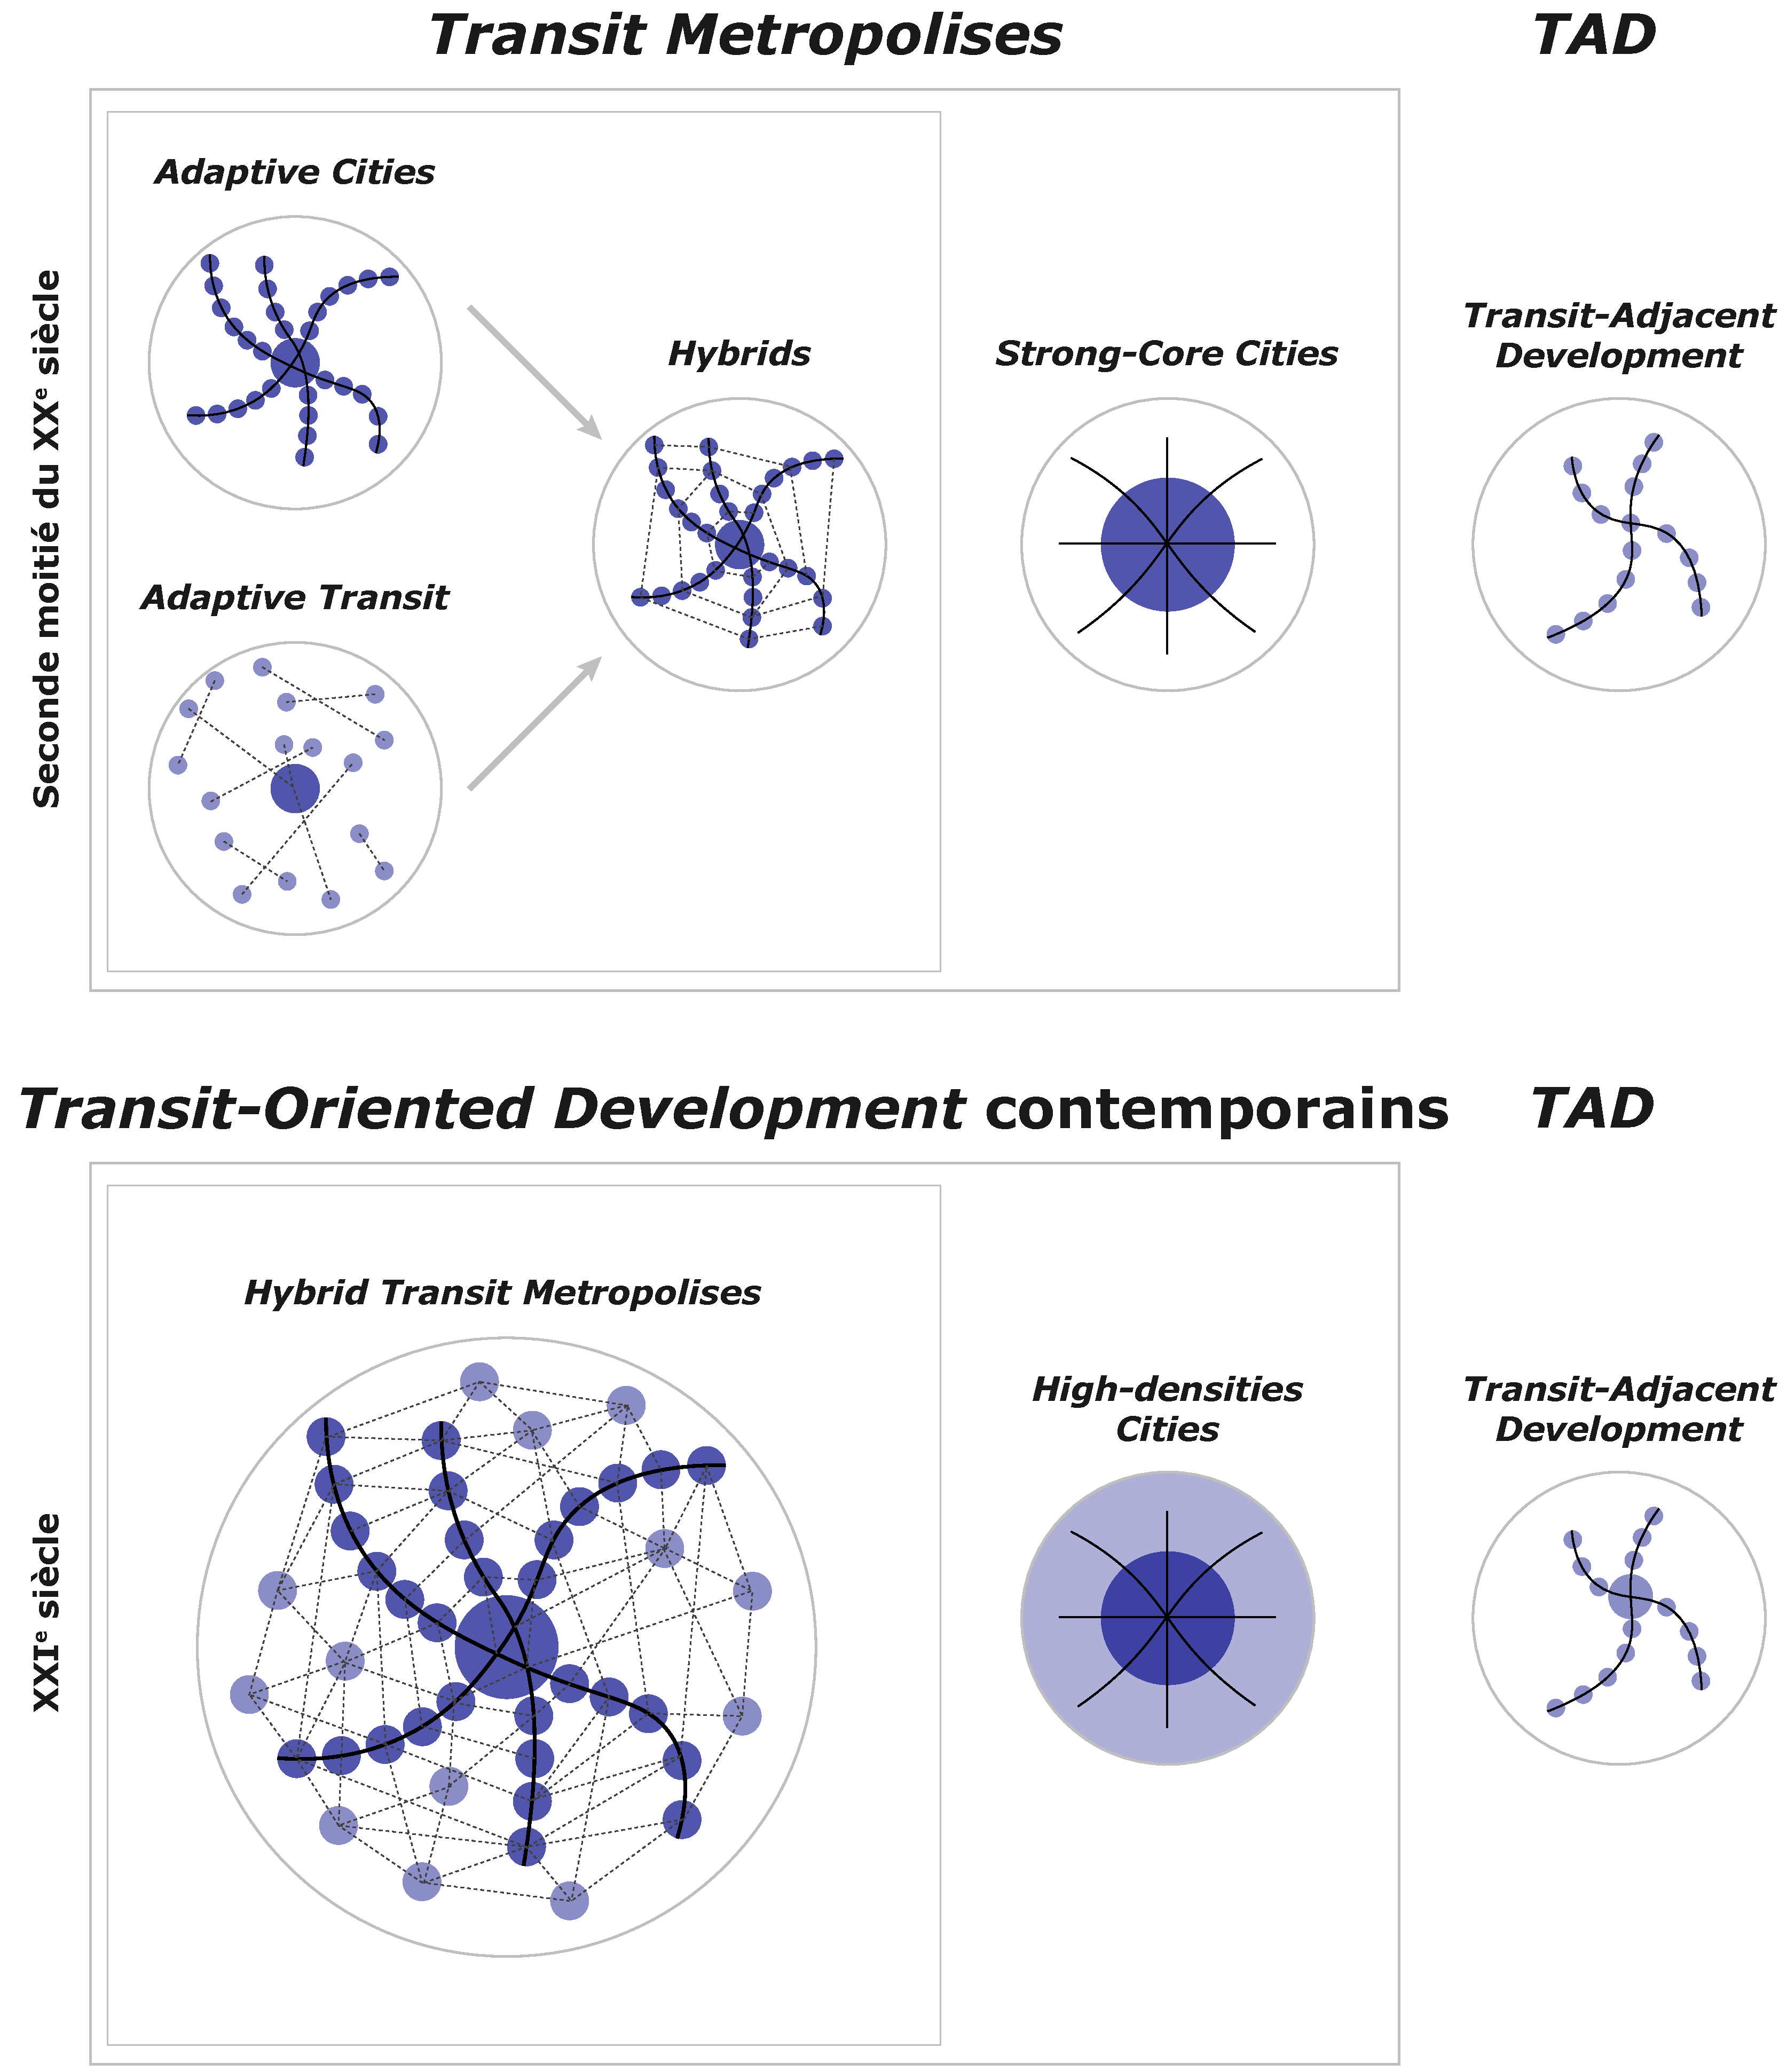
\includegraphics[width=1\columnwidth]{src/Figures/Chap-1/FR_Schema_Alternative_cities_transit.pdf}}
        \vspace{5pt}
        \begin{flushright}\scriptsize{
        Sources~: \textcolor{blue}{\textcite[3]{vos_influence_2014}}\index{Vos, Jonas de|pagebf}\index{Acker, Veronique van|pagebf}\index{Witlox, Frank|pagebf} et \textcolor{blue}{\textcite[2]{liu_historical_2024}}\index{Liu, Yudi|pagebf}\index{Manabe, Rikutaro|pagebf}\index{Nitanai, Ryoichi|pagebf}\index{Murayama, Akito|pagebf}
        \\
        Adaptation graphique~: \textcolor{blue}{Dylan Moinse (2025)}
        }\end{flushright}
    \end{carte}
    
    % Adaptive Transit
Les \textsl{Adaptive Transit}, caractérisées par un étalement urbain plus prononcé, ont choisi d'inverser le raisonnement entre croissance urbaine et réseaux de transport. Pour desservir efficacement des territoires périurbains à faible densité, les systèmes de mobilité doivent s’adapter aux formes urbaines dispersées de ces espaces. \textcolor{blue}{Susan} \textcolor{blue}{\textcite[108]{handy_reviews_1999}}\index{Handy, Susan|pagebf} met en lumière cette problématique, selon laquelle les villes étasuniennes, fortement marquées par l’étalement urbain, ne peuvent s’inspirer directement des expériences des \textsl{Adaptive Cities} et doivent plutôt adopter un modèle basé sur le format des \textsl{Adaptive Transit}. Dans ces contextes urbains, les déplacements régionaux suivent moins une logique radiale que des flux tangents, reliant les périphéries entre elles (voir la \hyperref[fig-chap1:schema-transit-metropolis]{carte~\ref{fig-chap1:schema-transit-metropolis}}, page~\pageref{fig-chap1:schema-transit-metropolis}). Cependant, les réseaux de transport en commun conventionnels sont souvent organisés autour d’itinéraires fixes et radiaux, ou parfois diamétraux, ce qui limite leur capacité à répondre à ces besoins. Les solutions proposées par ce type de \textsl{Transit Metropolis}, également désignées par l’acronyme \acrfull{DOT}, s’appuient sur des innovations technologiques et servicielles pour offrir une flexibilité accrue, en mesure de concurrencer la voiture individuelle \textcolor{blue}{\autocite[132]{cervero_transit_2020}}\index{Cervero, Robert|pagebf}. L’objectif de ces systèmes est de promouvoir une mobilité alternative au modèle auto-centré, tout en proposant des services de transport aux caractéristiques proches de la voiture \textcolor{blue}{\autocite[67-68]{bourdin_major_2024}}\index{Bourdin, Alain|pagebf}. Ces solutions misent sur des trajets personnalisés, adaptés aux défis des \Guillemets{premiers et derniers kilomètres} ainsi qu’aux besoins de déplacement \Guillemets{porte-à-porte}. Ces services basés sur la demande se positionnent comme des compléments au transport public traditionnel en renforçant leur attractivité et leur accessibilité. Les \textsl{Adaptive Transit} peuvent être illustrées par le système de tram-train de Karlsruhe, mis en service en 1992\footnote{
    Confrontée à un processus de périurbanisation important et à un manque de coordination entre les agences de transport public, la ville de Karlsruhe n’a pas su initialement optimiser l’utilisation de son réseau de transport urbain \textcolor{blue}{\autocite[p.~343-360 (chapitre 13)]{cervero_transit_1998}}\index{Cervero, Robert|pagebf}. Pour répondre à cette problématique, un projet adapté à son contexte territorial voit le jour~: la conception d’un système de tram-train interconnecté, connu sous le nom de \textsl{Zweisystem-Stadtbahn}. La première ligne de ce système dessert le centre-ville de Karlsruhe en mode tramway, puis emprunte les voies ferrées interurbaines pour rejoindre Bretten. Ce projet, testé en 1986 avant son inauguration en 1992, tend à offrir une solution efficace aux besoins de mobilité périurbaine. La mise en service de cette ligne pilote, qui a rapidement vu sa fréquence augmenter, a permis d’atteindre les objectifs escomptés, à savoir la multiplication par quatre de sa fréquentation, dont une majorité d'ancien·ne·s automobilistes \textcolor{blue}{\autocite[41]{beaucire_reseau_2000}}\index{Beaucire, Francis|pagebf}. Au-delà de ses aspects purement techniques, le \Guillemets{modèle de Karlsruhe} suscite aujourd’hui un vif intérêt \textcolor{blue}{\autocite[41]{beaucire_reseau_2000}}\index{Beaucire, Francis|pagebf}. Ce système offre une réponse adaptée à un contexte urbain hétérogène en captant efficacement les territoires périurbains qui, jusqu’alors, n’ont pas été pensés pour être intégrés aux réseaux de transport public \textcolor{blue}{\autocite[57-65]{grisot_manifeste_2020}}\index{Grisot, Sylvain|pagebf}. Ce système technique et tarifaire unique permet aux habitant·e·s des zones périurbaines de rejoindre directement les centres urbains sans nécessiter de rupture de charge, les dispensant d’un \gls{détour} par la gare, souvent excentrée. En parallèle, pour les collectivités locales et les opérateurs de transport, ce modèle représente une promesse d’investissement moins coûteux, grâce à la réutilisation des infrastructures existantes \textcolor{blue}{\autocite[17]{lhostis_multi-criteria_2017}}\index{L'Hostis, Alain|pagebf}\index{Soulas, Claude|pagebf}\index{Vulturescu, Bogdan|pagebf}.
}~; le système de bus guidé d'Adélaïde, complètement opérationnel depuis 1989\footnote{
    La ville d’Adélaïde connaît une situation similaire à celle de Karlsruhe, marquée par un phénomène d'extension urbaine considérable \textcolor{blue}{\autocite[p.~362-377 (chapitre 14)]{cervero_transit_1998}}\index{Cervero, Robert|pagebf}. Face à la croissance urbaine très rapide de banlieues situées au nord-est de l'agglomération, les pouvoirs publics choisissent dans un premier temps d’étendre le réseau de tramways existant, avant de se tourner vers une solution alternative~: la mise en place d’un système de bus guidé. Ce système, connu sous le nom d'\textsl{O-Bahn}, est le premier de ce type au monde et reste, à ce jour, le plus long réseau en service. Il constitue une hybridation entre le bus conventionnel et le transport sur rail \textcolor{blue}{\autocite[143]{currie_assessing_2014}}\index{Currie, Graham|pagebf}\index{Delbosc, Alexa|pagebf}. Le \textsl{O-Bahn} repose sur l’utilisation de roues latérales spécifiques, qui permettent au \acrshort{BHNS} de circuler sur des voies dédiées en site propre, rendant le voyage à la fois plus rapide et sécurisé \textcolor{blue}{\autocite[2]{currie_bus_2006}}\index{Currie, Graham|pagebf}. Ce système est conçu pour relier efficacement le \acrfull{CBD} de la ville à la nouvelle centralité commerciale et urbaine de Tea Tree Plaza, située dans une banlieue en pleine expansion. Lors de son lancement, le \textsl{O-Bahn} comptait 6 kilomètres de voies en 1986, étendus à 12 kilomètres en 1989. L’objectif principal est alors de décongestionner le réseau autoroutier en offrant un service performant, souple et relativement peu coûteux. Le réseau \textsl{O-Bahn} atteint ainsi une vitesse commerciale moyenne de 80 kilomètres par heure, en faisant le système de bus le plus rapide au monde \textcolor{blue}{\autocite[3]{currie_bus_2006}}\index{Currie, Graham|pagebf}. Ce succès est attribuable à l’infrastructure dédiée et à l’espacement important entre les arrêts, à hauteur de cinq kilomètres environ. Par ailleurs, le taux d’occupation des bus guidés est généralement deux fois supérieur à celui des bus classiques de l’agglomération, tandis que les coûts d’exploitation par passager·ère et par kilomètre sont inférieurs d’un tiers à ceux des bus réguliers \textcolor{blue}{\autocite[7]{basbas_advances_2005}}\index{Basbas, Socrates|pagebf}. Actuellement, 18 lignes utilisent l’alignement de 12 kilomètres, bien que seules 8 d’entre elles l’exploitent dans son intégralité \textcolor{blue}{\autocite[3]{rogers_o-bahn_2002}}\index{Rogers, Lee~H.|pagebf}. Ce système illustre comment une région confrontée à une périurbanisation notable a choisi non pas de contenir cette dynamique urbaine, mais de la connecter à son centre urbain. L’infrastructure du \textsl{O-Bahn} est de plus en mesure de traverser des quartiers denses sans nécessiter d’importantes reconfigurations de l'espace. Cependant, malgré le succès populaire et même touristique de ce système, Adélaïde reste dominée par l’automobile. Cette prédominance se reflète également parmi les usager·ère·s du \textsl{O-Bahn}, dont plus de la moitié accèdent aux arrêts en voiture, nécessitant un élargissement récurrent des infrastructures de \acrfull{P+R}. Ces extensions interviennent malgré les efforts initiaux d'aménagement piétonnier et cyclables autour des stations \textcolor{blue}{\autocite[11]{currie_bus_2006}}\index{Currie, Graham|pagebf}.
}~; ou le système de \textsl{paratransit}, appelé \textit{microbús}, présent à Mexico City\footnote{
    À Mexico City, le décalage significatif entre l’offre de transport en commun et l’étendue de la surface urbanisée a favorisé l’émergence de stratégies autorégulées initiées par le marché. C’est dans ce contexte qu’a vu le jour, dans les années 1970, le service de transport privé de \textsl{microbús}, également appelé \textsl{pesero}. Ce système s’est spontanément développé pour répondre aux besoins de mobilité identifiés dans les territoires non desservis par le réseau de transport public \textcolor{blue}{\autocite[p.~379-399 (chapitre 15)]{cervero_transit_1998}}\index{Cervero, Robert|pagebf}. Ainsi, le marché a su s’adapter pour combler l’écart entre une demande croissante de mobilité et une offre insuffisante en matière d'infrastructure et de service de mobilité. Face à l’expansion rapide de l’aire urbaine de Mexico City, le \textsl{paratransit} a su trouver sa place dans le système de mobilité en coexistant en tant que mode de transfert. Ce service permet de transporter les populations enclavées vers les stations de transport public situées en périphérie du centre. Fonctionnant comme des taxis collectifs, ces véhicules, souvent des voitures à l’origine, suivent un tracé de ligne fixe, similaire à celui d’une ligne de bus. Ils prennent et déposent des passager·ère·s à la demande le long de l'\gls{itinéraire} \textcolor{blue}{\autocite[4]{chiu_does_2022}}\index{Chiu, Bing-yu|pagebf}. Ce système \Guillemets{informel} joue un rôle clé en tant que service de rabattement auto-organisé, comme le confirme la littérature existante \textcolor{blue}{\autocite[98, 246]{adjeroud_coexistence_2024}}\index{Adjeroud, Heythem|pagebf}\index{Chapelon, Laurent|pagebf}\index{Lammoglia, Adrien|pagebf}. Il présente notamment l'avantage de ne pas nécessairement requérir d'investissements publics. Cependant, il peut représenter une concurrence directe au transport public \Guillemets{formel} et tout autant contribuer à l’étalement urbain \textcolor{blue}{\autocite[4]{chiu_does_2022}}\index{Chiu, Bing-yu|pagebf}. Sur cette base, \textcolor{blue}{Edzani} \textcolor{blue}{\textcite[65]{libunyu_paratransit-oriented_2024}}\index{Libunyu, Edzani|pagebf} identifie une forme de \textsl{Paratransit-Oriented Transit-Oriented Development}, en prenant le cas de Mexico City comme exemple.
} \textcolor{blue}{\autocite[343-399]{cervero_transit_1998}}\index{Cervero, Robert|pagebf}.%%Rédigé%%

    % Hybrides
En laissant volontairement de côté les \textsl{Strong-core Cities}, qui reposent sur des dynamiques de revitalisation urbaine et qui s’éloignent de notre problématique centrale, nous nous concentrons sur le quatrième et dernier type de \textsl{Transit Metropolis}~: les \textsl{Hybrids}, qui revêtent un intérêt particulier dans le cadre de notre recherche. Dépassant la dichotomie entre \textsl{Adaptive Cities} et \textsl{Adaptive Transit}, ces \textsl{Hybrids} s’affirment par leur aptitude à tirer parti des points forts des deux concepts. Cette approche aspire à trouver un juste équilibre entre un urbanisme dense et mixte concentré sur les corridors bien desservis et un système de mobilité alternative efficace, destiné à couvrir les périphéries à plus faible densité. Ce compromis est illustré par la \hyperref[fig-chap1:schema-transit-metropolis]{carte~\ref{fig-chap1:schema-transit-metropolis}} (page~\pageref{fig-chap1:schema-transit-metropolis}). Ces \textsl{Hybrids} regroupent, en un même territoire, les solutions de mobilité et d’urbanisme issues des deux types de \textsl{Transit Metropolis} décrits précédemment. Ils se rapprochent ainsi d’un modèle polycentrique, caractérisé par une hiérarchie de centres urbains interconnectés par des lignes structurantes. L’accessibilité de ces centres est renforcée par des services de mobilité flexibles, répondant aux besoins des zones périurbaines et faiblement denses \textcolor{blue}{\autocite[213-295]{cervero_transit_1998}}\index{Cervero, Robert|pagebf}.%%Rédigé%%
    
    % Hybrid Transit Metropolises
Cette typologie de \textsl{Transit Metropolises}, \textcolor{blue}{Robert} \textcolor{blue}{\textcite[131]{cervero_transit_2020}}\index{Cervero, Robert|pagebf} la réinterprète finalement sous la désignation consolidée de \textsl{Hybrid Transit Metropolises}. Une telle relecture permet de démontrer comment ces territoires ont transcendé la dichotomie entre \textsl{Adaptive Cities} et \textsl{Adaptive Transit}, une dualité qui a aujourd’hui perdu de sa consistance. Ce constat renvoie aux \textsl{Hybrids}, telles que décrites par \textcolor{blue}{\textcite[213-295]{cervero_transit_1998}}\index{Cervero, Robert|pagebf} vingt ans plus tôt, bien que revisitées à la lumière des évolutions contemporaines des systèmes de mobilité. Le facteur déterminant de cette révision réside dans l’émergence et la généralisation des \acrshort{NTIC}, ayant engendré simultanément une \Guillemets{mobilité intelligente} (\textsl{smart mobility}) et un \Guillemets{urbanisme intelligent} (\textsl{smart cities}). Par ailleurs, les pratiques et les imaginaires de mobilité des nouvelles générations ont considérablement évolué, influençant les formes de déplacement et les attentes en matière d’accessibilité. Derrière ces concepts, parfois assimilés à des \Guillemets{mots-valises}, \textcolor{blue}{\textcite[137-143]{cervero_transit_2020}}\index{Cervero, Robert|pagebf} plaide pour une approche intégrative en dépassant les clivages au profit de \Guillemets{\textsl{Transit Metropolises} du XXI\textsuperscript{e} siècle}. Au terme de son analyse, l'auteur observe une convergence des territoires vers les \textsl{Hybrid Transit Metropolises}, où la maîtrise des formes urbaines, en adéquation avec les principes du \acrshort{TOD}, s'associe au développement d'un éventail de solutions de mobilité flexibles et \Guillemets{porte-à-porte} (voir la \hyperref[fig-chap1:schema-transit-metropolis]{carte~\ref{fig-chap1:schema-transit-metropolis}}, page~\pageref{fig-chap1:schema-transit-metropolis}). Ces métropoles intègrent alors des systèmes de \textsl{micro-transit}~–~\textcolor{blue}{\textcite[144]{cervero_transit_2020}}\index{Cervero, Robert|pagebf} évoque notamment les exemples de la marche, du vélo ou encore des services de \acrfull{VTC}, de \acrfull{VLS}, de \acrfull{VFF}, de \acrfull{TEFF}, de \textsl{paratransit} et de taxi autonome~–~en complément de leurs infrastructures de transport en commun à grande capacité ou de \textsl{mass transit} \textcolor{blue}{\autocite[7]{thomas_transit-oriented_2020}}\index{Thomas, Ren|pagebf}\index{Bertolini, Luca|pagebf}. Parallèlement, elles adoptent une gestion \Guillemets{intelligente} de la demande (\textsl{smart pricing}). Dans cette optique, le mot d’ordre de ces \acrshort{TOD}\textcolor{blue}{s} contemporains repose sur l’élaboration d’une offre multimodale synergique, qui tire parti des avancées des \acrshort{NTIC} et de la généralisation des \textsl{smartphones}, avec pour finalité de limiter la dépendance automobile.%%Rédigé%%

    % Approches offre et demande
Les \textsl{Hybrid Transit Metropolises} s’appuient sur des éléments structurants issus d’une double approche, par l’offre (\acrshort{TSM}) et par la demande (\acrshort{TDM}) de mobilité, telle que décrite par \textcolor{blue}{\textcite[67]{cervero_transit_1998}}\index{Cervero, Robert|pagebf} avant d'être renouvelée \textcolor{blue}{\autocite[137-143]{cervero_transit_2020}}\index{Cervero, Robert|pagebf}~:
    \begin{customitemize}
\item D’une part, l’approche \acrshort{TSM} repose sur les \Guillemets{3Ds}~: densité, diversité et \textsl{design}. Elle inclut également le développement de modes de déplacement non motorisés, tels que l’usage intermodal du vélo. Les \acrshort{NTIC} jouent un rôle clé dans cette dynamique en promettant de transformer à la fois les modalités de déplacement et les environnements dans lesquels s’inscrivent les flux. Cela passe par l’essor du télétravail, des visioconférences et du commerce en ligne, mais aussi par l’optimisation des flux grâce à des outils tels que la gestion de trafic via la signalisation intelligente, la géolocalisation des véhicules, les données en temps réel pour les passager·ère·s, ou encore les péages automatisés en milieu urbain. Un exemple emblématique est celui de Copenhague, dont le réseau cyclable de renommée mondiale s’inscrit dans une politique de \acrshort{TOD} hybride. Dans un premier temps, nous l'avons vu, la capitale danoise a misé sur un réseau ferroviaire performant allié à une croissance urbaine concentrée dans des corridors denses. C'est par la suite qu'elle a développé des infrastructures cyclables de grande qualité pour répondre aux flux tangents, en périphérie urbaine. Le vélo y est pleinement intégré à la stratégie de \acrshort{TOD}, avec des infrastructures abondantes de stationnement à proximité des stations de transport en commun, des voitures dédiées à l'emport du vélo dans les trains et le développement de 26 autoroutes cyclables (\textsl{Cycle Super Highways}) totalisant plus de 500 kilomètres. Par ailleurs, des services de \acrshort{VLS} et de \acrshort{VFF} complètent cette offre~;
\item D’autre part, au lieu de simplement chercher à améliorer la mobilité à moindre coût, l’approche \acrshort{TDM} vise à optimiser l’utilisation des ressources existantes en influençant, voire en réduisant, la demande de mobilité. Un consensus croissant souligne que la gestion du stationnement automobile constitue l’une des stratégies basées sur cette demande parmi les plus efficaces, bien qu’elle demeure sensible des points de vue des négociations politiques et de l'acceptabilité sociale. Cette démarche peut prendre la forme de l'introduction de frais de stationnement, du développement du covoiturage ou de la promotion du télétravail. Des mesures complémentaires, telles que la régulation de l’usage automobile par le biais de la réduction ou de l’interdiction du trafic motorisé dans certaines zones, le ralentissement de la circulation, ou encore l’augmentation des coûts liés à l’usage automobile (carburant, charges de congestion ou taxes carbone), viennent renforcer cette approche. Séoul constitue un exemple convaincant, où des politiques volontaristes en faveur du \acrshort{TOD} se sont traduites par la mise en place d’un réseau de 120 kilomètres de \acrshort{BHNS} en 2017. Cette initiative s’est accompagnée de la reconversion de quartiers centrés sur l’automobile en espaces piétonniers \textcolor{blue}{\autocite[6]{prayogi_bus_2018}}\index{Shin, Dooho|pagebf}, le projet emblématique étant sûrement la restauration de la rivière Cheonggyecheon en 2003, jusqu'alors transformée en autoroute urbaine \textcolor{blue}{\autocite[]{shin_cheongyecheon_2013}}\index{Shin, Dooho|pagebf}.
    \end{customitemize}%%Rédigé%%

    % E-TOD
Cette réflexion sur une révision des principes du \acrshort{TOD} entre en résonance avec le concept décliné d'\acrfull{E-TOD}, développé par le chercheur en urbanisme et en génie civil \textcolor{blue}{\textcite{schneider_illustrating_2012}}\index{Schneider, Jerry~B.|pagebf}. Ce concept envisageait déjà la promesse de bénéfices issus de l’intégration des technologies pour enrichir le modèle urbain originel. Le postulat de base repose sur un constat également observable dans les \textsl{Transit Metropolises}, en particulier du côté des \textsl{Adaptive Transit} et des \textsl{Hybrids}. Ce sont des territoires présentant un tissu urbain largement étalé et fragmenté, difficilement desservi par les réseaux de transport en commun conventionnels, et qui pose la problématique fondamentale des \Guillemets{premiers et derniers kilomètres} du transport public \textcolor{blue}{\autocite[133]{cervero_transit_2020}}\index{Cervero, Robert|pagebf}. À cette fin, \textcolor{blue}{\textcite[141]{schneider_prt_1992}}\index{Schneider, Jerry~B.|pagebf} propose une vision du \acrshort{TOD} attentive à la fonction d’intermodalité et de connexion. Cette approche gagnerait à intégrer un système de transport moyennement capacitaire et doté d’une capillarité accrue, incarné par ce qu’il nomme le \acrfull{PRT}\footnote{
    Le \acrfull{PRT}, ou \textsl{Personal Rapid Transit}, est un système de transport, souvent automatisé et sur site propre, mettant en circulation des capsules individuelles ou de faible capacité, conçues pour transporter des individus ou de petits groupes directement vers leur destination. Ce service de mobilité se situe à mi-chemin entre le transport en commun conventionnel et les modes de déplacement individuels. Le \acrshort{PRT} est une forme de transport à la demande~: les voyageur·se·s sélectionnent leur destination, et le véhicule effectue un trajet direct sans arrêt intermédiaire, à la différence des systèmes de transport public classiques soumis à des arrêts réguliers et à des horaires fixes. Cette configuration permet, en théorie, de réduire les temps d’attente et de parcours. Par ailleurs, le \acrshort{PRT} nécessite une emprise au sol relativement réduite, ce qui le rend particulièrement adapté aux environnements urbains denses. Cependant, ce système présente également plusieurs limites. Il se heurte à la complexité de son intégration dans les réseaux de transport existants, à des coûts initiaux très élevés pour la construction des infrastructures et la mise en œuvre des services dédiés, ainsi qu’à une capacité limitée, ce qui restreint son efficacité dans les contextes à forte demande. En pratique, très peu de projets de \acrshort{PRT} ont été réalisés et surtout commercialisés. La majorité des prototypes sont restés à l’état de projets expérimentaux.
}. L’enjeu ici ne réside pas dans une substitution du transport public par le \acrshort{PRT}, mais bel et bien dans la facilitation de l’accès aux gares ferroviaires pour des zones situées au-delà de la portée socialement acceptable de la marche combinée. La méthode \acrshort{E-TOD} porte une stratégie d'interconnexion inter-urbaine, associant les mécanismes d'un système global \acrfull{F-D-C} destiné à relier l'ensemble des modes collectifs\footnote{
    Le concept de \acrfull{F-D-C} désigne une stratégie de structuration des réseaux de transport reposant sur trois fonctions complémentaires. Ce modèle est fréquemment utilisé dans la planification des systèmes de transport urbain et régional, car il offre une organisation cohérente et hiérarchisée des flux de mobilité. Les trois composantes principales de ce modèle se déclinent comme suit~:
        \begin{customitemize}
    \item \textsl{Alimentation} (\textsl{Feeder}). Cette fonction concerne les infrastructures ou les services dédiés à la collecte des passager·ère·s dans des zones périphériques ou éloignées, pour les acheminer vers des points d’accès stratégiques du réseau principal~;
    \item \textsl{Distribution}. Une fois les passager·ère·s arrivé·e·s dans un pôle d'échange multimodal, la fonction de distribution consiste à les transporter vers leur destination finale à l’intérieur de zones urbaines plus denses ou complexes. Dans ce contexte, le \acrshort{PRT} joue un rôle central dans la gestion de cette étape~;
    \item \textsl{Circulation}. La circulation concerne les déplacements internes à une zone spécifique, indépendamment des points centraux ou des lignes principales. Elle assure une mobilité de proximité, en particulier dans des quartiers ou des zones résidentielles.
        \end{customitemize}
}, avec l'intégration d'un système d'organisation désigné sous le terme d'\textsl{Urban Oasis}\footnote{
    L’\textsl{Urban Oasis} est un concept développé par l’architecte étasunienne \textcolor{blue}{Roxanne} \textcolor{blue}{\textcite{warren_urban_1997}}\index{Warren, Roxanne|pagebf}, qui propose un modèle d’aménagement urbain axé sur la création d’espaces verts et de lieux de détente au sein des zones fortement densifiées des métropoles. Ce concept s’inscrit dans une réflexion plus large sur les moyens de réintroduire la nature et de promouvoir le bien-être au cœur d’environnements urbains souvent marqués par une prédominance de surfaces minérales, d’infrastructures massives et d’une pression démographique accrue. Cette vision met l’accent sur la nécessité de réinscrire une échelle humaine dans des espaces urbains parfois perçus comme déshumanisés, de mettre à disposition des lieux de repos, de loisirs et de reconnexion avec la nature, ainsi que d'intégrer les principes d’écologie urbaine. En revalorisant les qualités environnementales et sociales des espaces urbains, l’\textsl{Urban Oasis} aspire à améliorer la qualité de vie des habitant·e·s tout en favorisant un urbanisme durable et résilient.
} \textcolor{blue}{\autocite[145]{schneider_prt_1992}}\index{Schneider, Jerry~B.|pagebf}. En somme, l'idée novatrice de ce système intermodal, conçu selon les principes caractéristiques du \acrshort{TOD}, réside dans la proposition de regrouper les clusters urbains pour les connecter au réseau de transport, par l'intermédiaire du réseau secondaire de \acrshort{PRT}, selon le principe de \Guillemets{\textsl{cluster-and-connect}} (voir la \hyperref[fig-chap1:schema-e-tod]{carte~\ref{fig-chap1:schema-e-tod}}, page~\pageref{fig-chap1:schema-e-tod}).%%Rédigé%%

    % Figure schéma E-TOD
    \begin{carte}[h!]\vspace*{4pt}
        \caption{Carte abstraite de la stratégie \Guillemets{\textsl{cluster-and-connect}} proposée dans le cadre du \textsl{Extended Transit-Oriented Development}.}
        \label{fig-chap1:schema-e-tod}
        \centerline{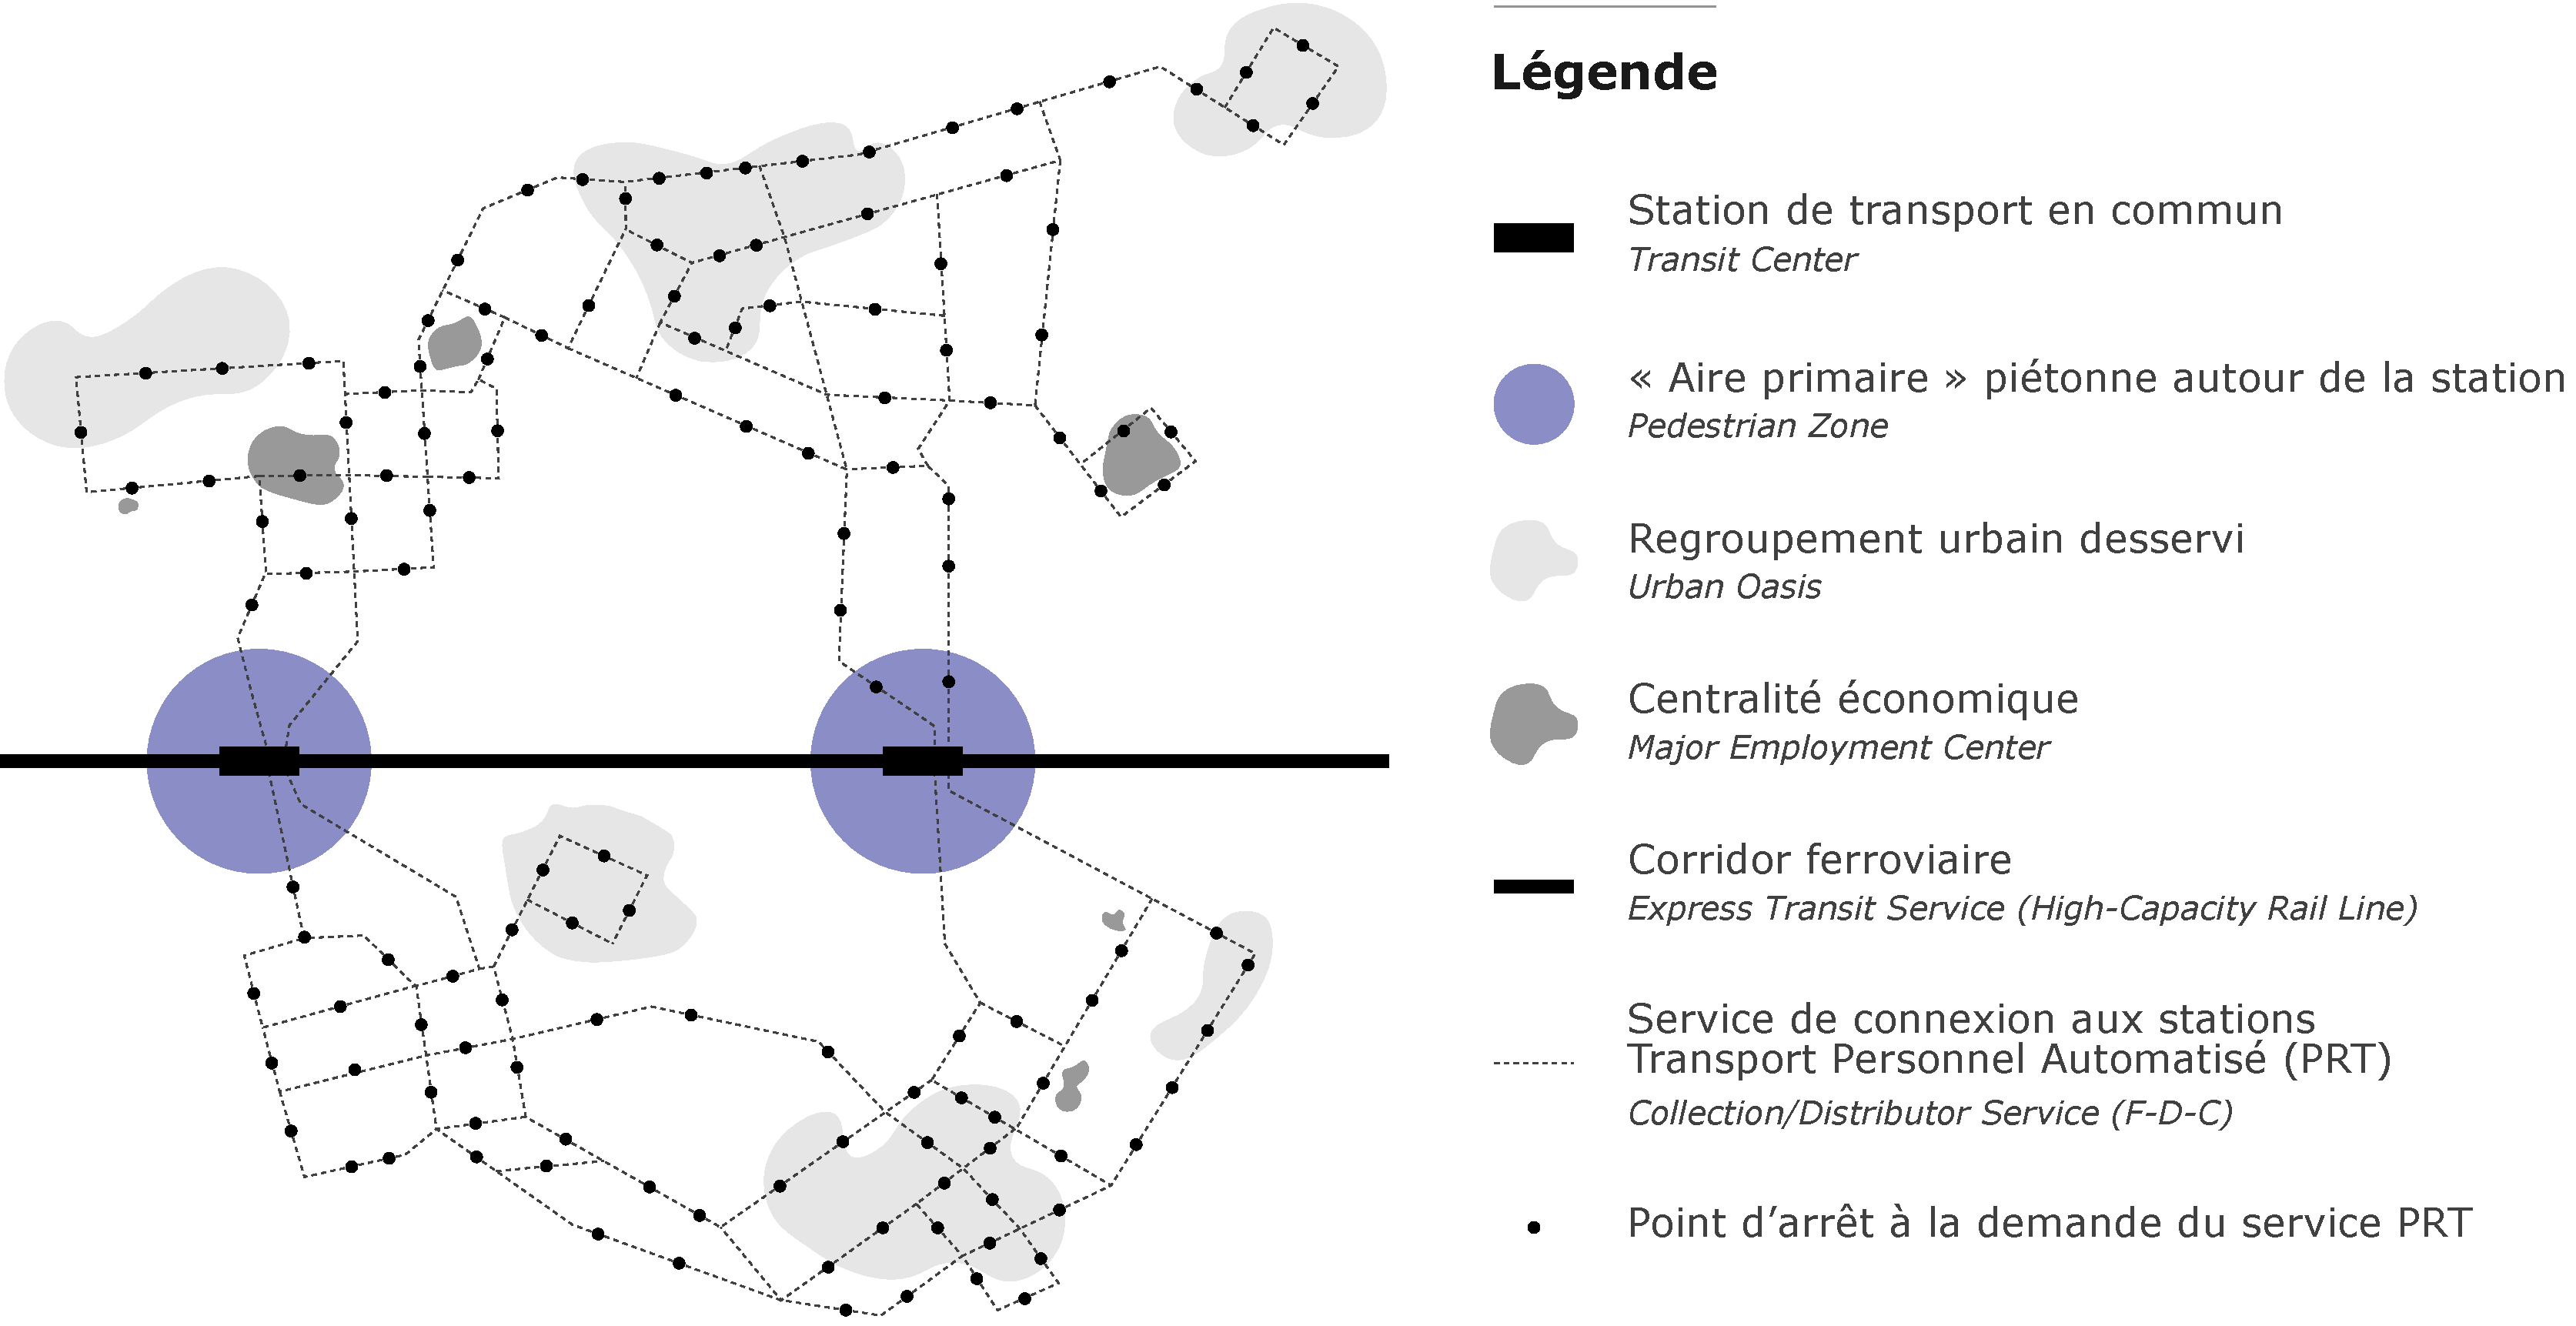
\includegraphics[width=1\columnwidth]{src/Figures/Chap-1/FR_Schema_Schneider.pdf}}
        \vspace{5pt}
        \begin{flushright}\scriptsize{
        Source~: \textcolor{blue}{\textcite[142]{schneider_prt_1992}}\index{Schneider, Jerry~B.|pagebf} (voir aussi \textcolor{blue}{\textcite{schneider_illustrating_2012}}\index{Schneider, Jerry~B.|pagebf})
        \\
        Adaptation graphique~: \textcolor{blue}{Dylan Moinse (2024)}
        }\end{flushright}
    \end{carte}

    % Limites E-TOD et Transition
Néanmoins, cette déclinaison du \acrshort{TOD}, bien qu’elle conserve les principes fondateurs du modèle, se heurte à des obstacles d’ordre technique, matériel et temporel. Le \acrshort{PRT} constitue à ce titre une solution infrastructurelle, particulièrement lourde d’un point de vue budgétaire et exigeante en termes de délais de mise en œuvre. Outre les défis technologiques qu’elle implique, le \acrshort{PRT} peine à offrir des gains intéressants en termes de réduction de la congestion, compromettant ainsi sa promesse de mobilité et d’urbanisme plus soutenables. Pour des raisons similaires, la voiture autonome partagée, qui s’inscrit de plus en plus dans les projections d’un urbanisme ferroviaire réactualisé, rencontre des problématiques comparables, alimentées par le mirage d'un bond en avant de la fréquentation du transport public\footnote{
    Dans sa thèse de doctorat, \textcolor{blue}{Félix} \textcolor{blue}{\textcite[333]{carreyre_are_2023}}\index{Carreyre, Félix|pagebf}\index{Coulombel, Nicolas|pagebf}\index{Bouillaut, Laurent|pagebf} s’est attaché à évaluer les performances des services basés sur le véhicule automatisé en mobilisant un cadre d’analyse coût-bénéfice combiné à une modélisation multi-agents avec \textsl{MATSim}. Ses travaux, menés dans les contextes berlinois et parisien, ont mis en évidence que l’introduction de taxis autonomes pourrait conduire à une aggravation de la congestion à Berlin. De surcroît, dans le cas de Saclay, un scénario intermodal associant ces services au système ferroviaire permettrait seulement d’accroître le taux d’occupation moyen des véhicules, bien que cela se fasse au détriment de l’usage du bus.
}. Dans ce contexte, le vélo apparaît comme une solution plus agile et plus concrète ayant fait ses preuves au sein des diverses \textsl{Hybrid Transit Metropolises} à travers le monde. Ce mode de déplacement individuel, naturellement \Guillemets{porte-à-porte} et à la demande, se révèle non seulement complémentaire au \acrshort{TOD}, mais également bien moins coûteux d'un point de vue économique et temporel. De plus, son intégration dans les politiques de mobilité urbaine repose sur des infrastructures relativement légères et adaptables. Dans cette perspective, une enquête menée par \textcolor{blue}{\textcite[119]{goletz_intermodality_2020}}\index{Goletz, Mirko|pagebf}\index{Haustein, Sonja|pagebf}\index{Wolking, Christina|pagebf}\index{L'Hostis, Alain|pagebf} à Berlin, Copenhague, Hambourg et Paris, soutient le potentiel intermodal du vélo dans le cadre d’un urbanisme orienté vers le rail. Les résultats montrent que les spécialistes et chercheur·se·s interrogé·e·s attribuent au vélo le rôle le plus prometteur pour connecter efficacement les infrastructures ferroviaires, à l’exception notable de Paris, où l’intermodalité avec les réseaux de transport en commun urbain est davantage plébiscitée. En s’appuyant sur la thèse des \textsl{Hybrid Transit Metropolises}, profondément renouvelées grâce aux innovations en matière de mobilité, cette recherche doctorale vise donc à examiner la place du vélo comme solution de mobilité pertinente pour répondre aux enjeux des \Guillemets{premiers et derniers kilomètres}. En cela, il s'agit dans le même temps d'explorer l’accompagnement progressif du retour en grâce du cycle par sa diversification modale, autour de ses déclinaisons, ainsi que la réintroduction de la trottinette, mise à jour par les avancées en électromobilité.%%Rédigé%%

     % ___________________________________________
    % 1.2.
    \newpage
    \needspace{1\baselineskip} % Réserve de l'espace
    \sectionheader{Regain de popularité de la mobilité individuelle légère}
\section{La (re)naissance d’une famille de véhicules légers désignés \Guillemets{mobilité individuelle légère}, aux contours mouvants
    \label{chap1:mobilite-individuelle-legere}
    }

    % Introduction
Cette section propose une lecture croisée des trajectoires évolutives de la \Guillemets{petite reine} et de la \Guillemets{nouvelle reine}, en adoptant une perspective historique. Elle met en lumière les moments clés de l’évolution technique et sociale de ces deux modes de déplacement. Nous allons notamment nous intéresser à comprendre comment et pourquoi ces cycles, longtemps considérés comme des objets de loisir, ont progressivement acquis une légitimité~–~encore en construction~–~dans les pratiques de mobilité quotidienne. Cette réhabilitation s’inscrit dans un contexte d’évolution des usages et des valeurs, mais aussi dans celui des innovations techniques et sociales, liées à des formes de \Guillemets{rétro-innovation} \textcolor{blue}{\autocite{barthelot_retro-innovation_2018}}\index{Barthelot, Bertrand|pagebf}. Bien que ces deux objets partagent une histoire marquée par des cycles de gain de popularité et de mise en retrait, ils connaissent aujourd’hui un renouveau, porté à la fois par des avancées techniques et par des transformations des pratiques urbaines. Comme le souligne \textcolor{blue}{Arnaud} \textcolor{blue}{\textcite[26]{passalacqua_monde_2011}}\index{Passalacqua, Arnaud|pagebf}, enseignant-chercheur et co-directeur de l'\acrfull{EUP}, la mobilité urbaine est un \Guillemets{\textsl{monde où les solutions nouvelles ne sont souvent que des reprises de formes anciennes et qui entretient~–~probablement involontairement~–~une confusion entre l'ancien et le contemporain, le passé et le futur. En se focalisant sur les véhicules souvent plus que sur les systèmes dans leur généralité, ce monde reste confus. Le vocabulaire employé, presque figé depuis le XIX\textsuperscript{e} siècle, contribue à renforcer cette confusion}}.%%Rédigé%%

    % Cycles d'innovation
Cette observation constitue une opportunité d’explorer les réflexions autour des \Guillemets{modèles} et des \Guillemets{cycles d’innovation} \textcolor{blue}{\autocite[]{schumpeter_theorie_1911}}\index{Schumpeter, Joseph Aloïs|pagebf}, tout en les inscrivant dans une perspective historique, philosophique et éthique. L’économiste autrichien et étasunien \textcolor{blue}{Joseph Aloïs} \textcolor{blue}{\textcite[107]{schumpeter_capitalisme_1942}}\index{Schumpeter, Joseph Aloïs|pagebf} illustre cette dynamique à travers son célèbre concept de \Guillemets{destruction créatrice}, moteur de la croissance économique par l’innovation dans les produits, procédés, modes de production, débouchés ou matières premières. Ce dernier observe que \Guillemets{\textsl{l'histoire des transports, depuis la diligence jusqu'à l'avion} [\dots] \textsl{constituent d'autres exemples du même processus de mutation industrielle} [\dots] \textsl{qui révolutionne incessamment de l'intérieur la structure économique, en détruisant continuellement ses éléments vieillis et en créant continuellement des éléments neufs.}}. Comme l'aborde le chercheur en philosophie politique et en histoire des idées \textcolor{blue}{Thierry} \textcolor{blue}{\textcite{menissier_innovations_2021}}\index{Ménissier, Thierry|pagebf} dans son ouvrage \textsl{Innovations~: Une enquête philosophique}, l’innovation ne se limite pas à répondre à des besoins préexistants~; elle agit également sur l’imaginaire collectif et suscite un intérêt pour le \textsl{différent}, dans l'intérêt d'accompagner des projets en devenir. Ainsi, il s’agit de réfléchir aux modalités permettant de mieux articuler le transfert et la territorialisation des innovations ainsi que leur mise en usage. Autrement dit, cela revient à interroger les conditions de leur déploiement à travers tous les segments de la société \textcolor{blue}{\autocite[5]{baron_thierry_2022}}\index{Baron, Nacima|pagebf}. Cette territorialisation des innovations a été étudiée par \textcolor{blue}{\textcite[13]{castex_prise_2017}}\index{Castex, Élodie|pagebf}\index{Frère, Séverine|pagebf}\index{Groux, Annette|pagebf}, notamment à travers la planification des transports. Leur étude appuie le décalage entre le lent infléchissement des acteurs publics dans la prise en compte des nouveaux modes de déplacement~–~tels que les \acrfull{STP}~–~dans les outils de gestion urbaine et de mobilité, et la rapidité des évolutions des besoins et des innovations portées par les acteurs privés.%%Rédigé%%

    % Annonce du plan
Dans cette section, nous nous engageons dans l'examen de l’évolution du vélo et de la trottinette, considérés à la fois comme des objets techniques et sociaux, ainsi que sur leur place et leurs usages dans les territoires, en fonction des contextes d’urbanisation (\hyperref[chap1:proximite-velo-trottinette]{section sur l'\Guillemets{âge d’or} de ces véhicules, suivi de leur déclin et de leur \Guillemets{retour}}, page~\pageref{chap1:proximite-velo-trottinette}). À partir de ce bref détour historique, nous mettrons en revue les principales innovations contemporaines ayant marqué ces véhicules, notamment leur électrification et leur mutualisation sous la forme d'une gestion partagée dans les espaces publics (\hyperref[chap1:velo-micromobilite-innovations]{section sur la diversification et l'\Guillemets{hybridation} modale des cycles}, page~\pageref{chap1:velo-micromobilite-innovations}). Enfin, nous contextualiserons la remise à l'honneur du vélo et de la trottinette, sous leurs diverses formes, dans une société \Guillemets{liquide}, portée par des générations de plus en plus adeptes de la \gls{multimodalité}. Ce cadre nous permettra également de proposer notre propre définition de cette famille de véhicules, en y délimitant des contours conceptuels plus précis. Cette définition vise à intégrer les véhicules que nous identifions comme ayant le plus grand potentiel stratégique pour renforcer et redéployer les principes du \acrshort{TOD} (\hyperref[chap1:caracterisation-mobilite-individuelle-legere]{section sur la caractérisation d’une classe de véhicules appelée \Guillemets{mobilité individuelle légère}}, page~\pageref{chap1:caracterisation-mobilite-individuelle-legere}).%%Rédigé%%

    % 1.2.1.
    \needspace{1\baselineskip} % Réserve de l'espace
\subsection{Évolution du \textsl{design} et de la place du cycle parmi les déplacements utilitaires
    \label{chap1:proximite-velo-trottinette}
    }

    % Introduction
Avant de s’imposer aujourd’hui comme des modes de déplacement urbain à part entière, le vélo et la trottinette ont traversé une évolution de plus d’un siècle, marquée à la fois par des innovations techniques et par des transformations des pratiques de mobilité et des imaginaires en Europe. Ces cycles ont connu, au fil de l’histoire, des paradigmes influencés par les constructions sociales associées aux véhicules \textcolor{blue}{\autocite[13]{heran_retour_2015}}\index{Héran, Frédéric|pagebf}. Différentes vagues successives ont contribué à les propulser progressivement parmi les pratiques de mobilité quotidiennes. Cette sous-section, consacrée à une chronologie succincte de leur évolution, a pour objectif de mieux resituer ces véhicules dans leur contexte historique et urbain. À cet effet, nous nous appuyons sur la lecture séquentielle proposée par l'historienne et sociologue française \textcolor{blue}{Catherine} \textcolor{blue}{\textcite[]{bertho-lavenir_voyages_2011}}\index{Bertho-lavenir, Catherine|pagebf}, construite autour de quatre époques dans l'évolution de la pratique du cycle~: \Guillemets{l'âge du vélocipède} ou l'invention mondaine (de 1814 aux années 1880)~; \Guillemets{l'âge de la bicyclette} ou le loisir bourgeois (des années 1880 à 1914)~; \Guillemets{l'âge du vélo} inscrit dans la mobilité quotidienne et touristique (de 1914 aux années 1970)~; et \Guillemets{l'âge de l'automobile} ou le vélo de sport et de loisir (depuis 1970). L’intention est d’offrir une lecture croisée du vélo et de la trottinette, qui partagent des origines communes et des trajectoires similaires. Ces deux familles de modes de déplacement ont notamment subi un sort comparable lorsque la ville moderne, avec son étalement spatio-temporel et l’augmentation des vitesses de déplacement, s’est construite autour de formes urbaines devenues inaccessibles et inadaptées pour ces véhicules.%%Rédigé%%

    % 1.2.1.1.
    \needspace{1\baselineskip} % Réserve de l'espace
\subsubsection*{\Guillemets{L'âge d'or} de la \Guillemets{petite reine}
    \label{chap1:proximite-velo-trottinette-chronologie}
    }

    % Vélo loisir bourgeois
\textsl{Les âges du vélocipède et de la bicyclette}. Les origines du vélo et de la trottinette peuvent être retracées à l’invention de la \Guillemets{machine à courir} (\textsl{Laufmaschine}), conçue en 1817 par le baron badois \textcolor{blue}{Karl Drais von Sauerbronn}\footnote{
    Ce dernier reprend l'idée du \Guillemets{céléripède}, littéralement \Guillemets{qui marche rapidement} de l'ingénieur français \textcolor{blue}{Joseph Nicéphore Niepce} \textcolor{blue}{\autocite{puech_bicyclette_2016}}\index{Puech, Chantal|pagebf}. En réalité, certaines inventions antérieures à celle communément attribuée au \Guillemets{père du vélo} révèlent que la conception de cet engin, reposant sur l’exploitation de la roue, remonte à plusieurs siècles. Parmi ces précurseur·se·s, \textcolor{blue}{Léonard de Vinci} a esquissé, autour des années 1490, les plans d’une machine en bois ressemblant au vélo moderne. Ce prototype comportait un siège, deux roues et des pédales, témoignant déjà d’une réflexion sur le déplacement individuel mécanisé \textcolor{blue}{\autocite[9]{hills_bicycle_2004}}\index{Hills, Larry|pagebf}.
}. Ce dernier souhaite développer un \Guillemets{carrosse sans chevaux} à la fois efficace et économique \textcolor{blue}{\autocite[24]{heran_retour_2015}}\index{Héran, Frédéric|pagebf}, l’origine de cette idée serait avant tout associée à une pénurie des chevaux, conséquence d'étés particulièrement froids. Ainsi, les racines du vélo coudoient celles de la trottinette à travers leur ancêtre commun, le \Guillemets{vélocipède}, connu sous le nom de draisienne en France et de \textsl{dandy-horse} en Angleterre\footnote{
    En 1818, une demande de brevet d'importation pour la \Guillemets{machine à courir} est déposée en France, sous la supervision de \textcolor{blue}{Louis-Joseph Dineur}. C’est également durant cette période que les premières draisiennes font leur apparition à Paris, accompagnées d’une campagne publicitaire remarquée et d’événements publics, tels que la première course organisée au jardin du Luxembourg \textcolor{blue}{\autocite[141]{kobayashi_histoire_1993}}\index{Kobayashi, Keizo|pagebf}. À cette époque, le terme \Guillemets{vélocipède} est utilisé de manière péjorative, notamment dans la presse et dans des spectacles comiques. Toutefois, ce mot a traversé les époques et est encore employé aujourd’hui pour désigner le vélo en bois qui n'a ni pédale, ni chaîne de transmission~; et utilisé par les enfants dans l’apprentissage de l’équilibre et de l’indépendance \textcolor{blue}{\autocite[21]{jouenne_quest-ce_2022}}\index{Jouenne, Noël|pagebf}.
} (voir l'\hyperref[fig-chap1:frise-chronologique-velo-trottinette]{illustration~\ref{fig-chap1:frise-chronologique-velo-trottinette}}, page~\pageref{fig-chap1:frise-chronologique-velo-trottinette}). Ce véhicule rudimentaire, composé de deux roues reliées par un cadre en bois et mis en mouvement par la force des pieds, rencontre un succès limité dans la sphère bourgeoise et finit par tomber dans un relatif oubli. Son poids et ses roues en bois peu stables le rendent en effet peu pratique. À partir de la fin du XIX\textsuperscript{e} siècle, le vélo et la trottinette prennent des trajectoires distinctes, marquant leur identité propre. D’un côté, la \Guillemets{Michaudine}, dotée de pédales ajoutées sur une draisienne dès 1861, popularise le vélo auprès des classes aisées (voir l'\hyperref[fig-chap1:frise-chronologique-velo-trottinette]{illustration~\ref{fig-chap1:frise-chronologique-velo-trottinette}}, page~\pageref{fig-chap1:frise-chronologique-velo-trottinette}), au travers de \textsl{clubs} de loisir et sportifs ainsi que de vélodromes \textcolor{blue}{\autocite[15-43]{dauncey_french_2012}}\index{Dauncey, Hugh|pagebf}. Cette évolution conduit au \Guillemets{véloce}, puis au \Guillemets{bicycle} en 1866, au \Guillemets{Grand-Bi} en 1871 et, enfin, au vélo moderne en 1891 \textcolor{blue}{\autocite[27]{heran_retour_2015}}\index{Héran, Frédéric|pagebf}. De l’autre côté, l’histoire de la trottinette est plus fragmentée~: elle émerge d’abord comme un jouet destiné aux enfants, dès 1895. À titre d’exemple, l’entreprise suisse \Marque{Wisa-Gloria AG}, fondée en 1882 et spécialisée dans les jouets, est l’une des pionnières dans la production de patinettes pour enfants \textcolor{blue}{\autocite{schweizerisches_nationalmuseum_draisine_2018}}\index{Schweizerisches Nationalmuseum@\textsl{Schweizerisches Nationalmuseum}|pagebf}. Les premières trottinettes à la forme proche de celles d’aujourd’hui apparaissent également à partir de 1895. Ces jouets, fabriqués en bois, sans moteur, sont équipés d’un guidon et de deux ou trois roues (voir l'\hyperref[fig-chap1:frise-chronologique-velo-trottinette]{illustration~\ref{fig-chap1:frise-chronologique-velo-trottinette}}, page~\pageref{fig-chap1:frise-chronologique-velo-trottinette}). Ils fonctionnent grâce à l’énergie humaine~: un pied repose sur la planche tandis que l’autre propulse l’utilisateur·rice par poussée au sol.%%Rédigé%%

    % Trottinette loisir bourgeois
En parallèle, les premiers modèles de patinette, destinés aux enfants des familles aisées, inaugurent une vague de trottinettes à deux roues commercialisées peu avant la Grande Guerre \textcolor{blue}{\autocite{jeux_et_compagnie_histoire_2013}}\index{Jeux et Compagnie@\textsl{Jeux et Compagnie}|pagebf}. Bien que la trottinette conserve initialement un statut de jouet, elle s’adresse progressivement à un public élargi, touchant des enfants issus de couches sociales moins privilégiées \textcolor{blue}{\autocite{historia_trottinette_2013}}\index{Historia@\textsl{Historia}|pagebf}. Durant l’entre-deux-guerres, des modèles métalliques dotés de pneumatiques apparaissent et sont brevetés, incorporant des innovations techniques inspirées par celles du vélo \textcolor{blue}{\autocite{arte_histoire_2014}}\index{Arte@\textsl{Arte}|pagebf}. Concernant leur rapport au monde social, tant le vélo que la patinette sont alors initialement associés à des pratiques bourgeoises\footnote{
    Bien que le premier développement du vélo ait été porté par les classes aisées, ces dernières ont ressenti une forme d’injustice liée à un manque de légitimité sur la route. Dans sa thèse de doctorat sur l’histoire des usages de la route, \textcolor{blue}{Jean} \textcolor{blue}{\textcite[126-132, 327]{orselli_usages_2008}}\index{Orselli, Jean|pagebf} met en lumière les défis auxquels les cyclistes ont été confrontés à la fin du XIX\textsuperscript{ème} siècle. Ces difficultés se manifestent à travers des réglementations marquées par une véritable \Guillemets{rage vélophobe}, ainsi que par des violences populaires, notamment en milieu rural, entre 1874 et 1896. Ces tensions précèdent l’instauration d’une réglementation nationale sur les vélocipèdes, dont l’application par les municipalités restera cependant peu respectée. Ce conflit doit être compris dans le contexte d’une route historiquement dominée par les voitures particulières attelées, qui jouissaient d’une place ancestrale et d’un respect tacite, aussi bien de la part de la population que de la police. Cette situation témoigne de la difficile acceptation sociale du vélo, dans une société où la voiture hippomobile incarnait encore, à cette époque, un moyen de locomotion prestigieux, utilisé par l’aristocratie française depuis des siècles \textcolor{blue}{\autocite[139]{orselli_usages_2008}}\index{Orselli, Jean|pagebf}.
}. Les prix élevés et les codes sociaux les réservent à une élite en quête de nouveaux loisirs et sports exclusifs \textcolor{blue}{\autocite[90]{bravard_cercle_2011}}\index{Bravard, Alice|pagebf}. Toutefois, avec la modernisation des procédés de fabrication et la démocratisation de ces objets\footnote{
    L'historien japonais \textcolor{blue}{Keizo} \textcolor{blue}{\textcite[149]{kobayashi_histoire_1993}}\index{Kobayashi, Keizo|pagebf}, dans son ouvrage intitulé \textsl{Histoire du vélocipède de Drais à Michaux 1817-1870. Mythes et réalités}, éclaire l'origine de la bicyclette en affirmant que \Guillemets{\textsl{parmi les principaux défauts du vélocipède, on reprochait au vélocipède la fatigue qu'il causait, son manque d'équilibre en marche ou à l'arrêt, l'inconfort dû aux trépidations.}}. Face à ces limites, diverses solutions techniques ont été envisagées pour pallier la fatigue liée à l’effort physique et améliorer l’expérience de l’utilisateur·rice. Les inventions de perfectionnement se multiplient, allant de l'amélioration de la transmission de l'énergie en améliorant la traction par la roue avant et la propulsion par la roue arrière, à la chaîne à maillon avec engrenage en 1829, l'ajout de bandages en caoutchouc plein en 1869 \textcolor{blue}{\autocites{inpi_draisienne_2020}[38]{jouenne_quest-ce_2022}}\index{Jouenne, Noël|pagebf}\index{INPI@\textsl{INPI}|pagebf}, ou encore l'invention du pneumatique à chambre à air en 1888 \textcolor{blue}{\autocite[14]{papon_retour_2012}}\index{Papon, Francis|pagebf}. Cependant, les avancées du vélocipède ne furent pas seulement d’ordre technique. Son développement social et culturel fut largement soutenu par des événements populaires, tels que des démonstrations publiques et des courses cyclistes, qui contribuèrent à sa visibilité et à son adoption progressive par un public plus large.
}, le vélo et la patinette finissent par s’étendre aux classes sociales plus modestes, perdant peu à peu leur caractère d'objet de distinction sociale, propre à une \Guillemets{culture bourgeoise}.%%Rédigé%%

    % Popularisation du vélo
\textsl{L'âge du vélo}. Durant la Belle Époque et plus encore durant les Années folles, le cyclotourisme s’impose comme une activité populaire en Europe, notamment grâce à l’organisation de tours à vélo prenant la forme de camps itinérants le week-end \textcolor{blue}{\autocite[26]{eskenazi_voir_2022}}\index{Eskenazi, Manon|pagebf}, mais aussi grâce à l'arrivée des premiers congés payés en 1936 \textcolor{blue}{\autocite[108]{dauncey_french_2012}}\index{Dauncey, Hugh|pagebf}. Les cyclistes peuvent alors stationner leurs vélos dans des auberges la nuit, une pratique qui se répand particulièrement en Allemagne \textcolor{blue}{\autocite[327]{herlihy_bicycle_2004}}\index{Herlihy, David|pagebf}. Entre 1918 et les années 1950, le vélo moderne se démocratise parmi les classes populaires, inaugurant une innovation sociale majeure~: celle des déplacements quotidiens à vélo, désormais perçus comme une alternative réaliste \textcolor{blue}{\autocite[31]{jouenne_quest-ce_2022}}\index{Jouenne, Noël|pagebf}. Ces déplacements pendulaires, notamment ceux des ouvrier·ère·s, permettent de réduire les temps de navette tout en offrant davantage de temps libre. Cette popularité s’amplifie durant la Grande Dépression, au cours des années 1930, en raison de la hausse du prix du carburant et de l’impossibilité, pour de nombreux ménages, d’accéder à la propriété automobile. Aux États-Unis, alors que le vélo était jusque-là considéré comme un véhicule pour enfant, celui-ci connaît alors un essor notable \textcolor{blue}{\autocite[327]{herlihy_bicycle_2004}}\index{Herlihy, David|pagebf}. Grâce à sa facilité d’usage et à sa vitesse, la demande et la production de vélo connaissent une forte croissance. Entre 1894 et 1934, le nombre de bicyclettes en circulation est multiplié par 32 \textcolor{blue}{\autocite[32]{papon_retour_2012}}\index{Papon, Francis|pagebf}. Dans de nombreux pays européens, le vélo devient le mode de déplacement dominant. À Copenhague, 33~\% de la population utilise le vélo en 1930, tandis qu’aux Pays-Bas, 3 millions de bicyclettes circulent, soit l’équivalent de la population. En France et au Royaume-Uni, environ 7 millions de vélos sont vendus, contre 15 millions en Allemagne. Le Japon comptabilise 6 millions d’usager·ère·s, tandis qu’aux États-Unis et en Chine, l’usage du vélo se développe progressivement \textcolor{blue}{\autocite[329]{herlihy_bicycle_2004}}\index{Herlihy, David|pagebf}. Dans ce contexte, des clusters industriels émergent. Saint-Étienne, par exemple, devient la \Guillemets{Capitale du Cycle}, avec plus d’une centaine d’usines produisant environ 80~\% des vélos fabriqués en France \textcolor{blue}{\autocite[328]{herlihy_bicycle_2004}}\index{Herlihy, David|pagebf}. Dans l’immédiat après-guerre, le vélo continue d’être massivement employé dans les villes européennes. La Suède, en particulier, s’affirme comme la première nation cycliste au monde.%%Rédigé%%

    % Popularisation vélo pliant
Il est impossible d’évoquer le vélo et les innovations techniques qui l'ont marqué sans mentionner le développement simultané du vélo pliant. Le premier brevet pour un vélo pliant est attribué à l’ingénieur étasunien \textcolor{blue}{Emmit G. Latta} en 1887, bien que des traces d’un Grand-Bi démontable remontent à 1878 \textcolor{blue}{\autocite{the_folding_cyclist_history_2010}}\index{The Folding Cyclist@\textsl{The Folding Cyclist}|pagebf}. Ce concept répondait au besoin de faciliter le stockage du vélo en réduisant son encombrement, bien qu'il sera principalement destiné à un usage militaire dans un premier temps\footnote{
    L’industriel français \textcolor{blue}{Charles Morel} développe un prototype de vélo pliant en 1892, qui, avec la collaboration du lieutenant \textcolor{blue}{Henri Gérard}, est à vocation militaire \textcolor{blue}{\autocite{the_folding_cyclist_history_2010}}. Présenté au Salon du Cycle à Paris en 1894, le modèle \Marque{Capitaine Gérard} est adopté par l’armée française et intègre les équipements de l’infanterie (voir l'\hyperref[fig-chap1:frise-chronologique-velo-trottinette]{illustration~\ref{fig-chap1:frise-chronologique-velo-trottinette}}, page~\pageref{fig-chap1:frise-chronologique-velo-trottinette}). Cette première génération de vélo pliant, présenté comme un atout face au cheval, est appelée la \Guillemets{Bicyclette pliante}. Sa capacité à se replier pour être portée sur le dos à l’aide de bretelles en fait une solution pratique qui ne nécessite pas d’infrastructures telles que des écuries ou des garages.
}. En France, la marque Peugeot commercialise un vélo pliant adulte léger, mais sans parvenir à en faire un produit véritablement populaire auprès du grand public \textcolor{blue}{\autocite{transportation_alternatives_folding_2013}}\index{Transportation Alternatives@\textsl{Transportation Alternatives}|pagebf}. La véritable réduction de la taille des roues du vélo pliant, inspirée notamment des vélos \Marque{Katakura} au Japon, ne se produit qu’à partir des années 1920, marquant le début de sa diffusion. Le vélo continue alors de bénéficier d'améliorations continues, avec le dépôt d’un brevet en 1944 pour un vélo pliant et démontable, équipé de roues de petite taille. Ce modèle, décrit par la presse de l’époque sous le nom de \Marque{Petit-Bi}, est présenté comme une avancée majeure \textcolor{blue}{\autocite[44]{jouenne_quest-ce_2022}}\index{Jouenne, Noël|pagebf}. La presse note que le \Marque{Petit-Bi} \Guillemets{\textsl{marquera une date dans l’histoire du cycle en raison des avantages certains qu’il présente}} \textcolor{blue}{\autocite{the_folding_cyclist_history_2010}}\index{The Folding Cyclist@\textsl{The Folding Cyclist}|pagebf}.%%Rédigé%%

    % Figure frise chronologique vélo trottinette
    \begin{figure}[h!]\vspace*{4pt}
        \caption{Évolution conjointe du vélo et de la trottinette dans une perspective historique.}
        \label{fig-chap1:frise-chronologique-velo-trottinette}
        \centerline{\includegraphics[width=1\columnwidth]{src/Figures/Chap-1/FR_Chronologie_velo_trottinette.pdf}}
        \vspace{5pt}
        \begin{flushright}\scriptsize{
        Photographie (A)~: \textcolor{blue}{\textcite{smithsonian_draisine_2006}}\index{Smithsonian@\textsl{Smithsonian}|pagebf}
        \\
        Photographie (B)~: \textcolor{blue}{\textcite{conservatoire_national_des_arts_et_metiers_velocipemichaux_2013}}\index{Conservatoire national des arts et métiers@\textsl{Conservatoire national des arts et métiers}|pagebf}
        \\
        Photographie (C)~: \textcolor{blue}{\textcite{chateau_de_compiegne_grand-bi_nodate}}\index{Château de Compiègne@\textsl{Château de Compiègne}|pagebf}
        \\
        Photographie (D)~: \textcolor{blue}{Kristy von} \textcolor{blue}{\textcite{moos_parcours_2019}}\index{Moos, Kristy von|pagebf}
        \\
        Photographie (E)~: \textcolor{blue}{\textcite{alienor_bicyclette_2015}}\index{Alienor@\textsl{Alienor}|pagebf}
        \\
        Photographie (F)~: \textcolor{blue}{Dylan Moinse (2023)}
        \\
        Photographie (G)~: \textcolor{blue}{\textcite{musee_national_suisse_draisienne_2018}}\index{Musée national suisse@\textsl{Musée national suisse}|pagebf}
        \\
        Photographie (H)~: \textcolor{blue}{\textcite{zerorider_lautoped_2023}}\index{Zerorider@\textsl{Zerorider}|pagebf}
        \\
        Auteur~: \textcolor{blue}{Dylan Moinse (2025)}
      }\end{flushright}
    \end{figure}

    % VAE
Qu’en est-il du \acrfull{VAE}~? Ses prémices remontent à seulement quinze ans après l’invention de la chaîne de vélo. Le premier prototype est attribué à \textcolor{blue}{Odgen Bolton Jr.}, qui, aux États-Unis, brevète en 1895 une draisienne équipée d’un moteur à courant continu à six pôles, intégré à la roue arrière et alimenté par une batterie de dix volts, quant à elle placée sous le tube horizontal du cadre \textcolor{blue}{\autocites[3]{hung_review_2020}{adelski_qui_2023}}\index{Hung, Nguyen Ba|pagebf}\index{Lim, Ocktaeck|pagebf}\index{Adelski, Adeline|pagebf}. La seconde génération de \acrshort{VAE} voit le jour en 1897 avec l’invention de \textcolor{blue}{Hosea W. Libbey}, qui conçoit le \Marque{Lampociclo}, un vélo équipé d’un double moteur électrique logé dans l’axe du pédalier. Le fonctionnement de cette innovation repose sur un générateur actionné par les pédales via une poulie et une courroie flexible. L’énergie produite alimente ensuite un petit moteur électrique \textcolor{blue}{\autocite[3]{hung_review_2020}}\index{Hung, Nguyen Ba|pagebf}\index{Lim, Ocktaeck|pagebf}. Toutefois, plusieurs tentatives d’amélioration échouent, notamment celle de la \Marque{Compagnie Parisienne}, qui développe un modèle de \acrshort{VAE} à la même époque, mais se heurte à des contraintes liées à un poids jugé excessif \textcolor{blue}{\autocite[78]{hadland_bicycle_2016}}\index{Hadland, Tony|pagebf}\index{Lessing, Hans-Erhard|pagebf}. À la fin de la Première Guerre mondiale, la société allemande \Marque{Heinzmann} inaugure la première production en série de moteurs électriques pour vélos, en équipant notamment les postier·ère·s du pays. Entre 1935 et 1937, le premier modèle de série, le \Marque{EMI/Philips}, est commercialisé, mais sa performance reste limitée face à la concurrence de l’automobile \textcolor{blue}{\autocite[143]{smethurst_bicycle_2015}}\index{Smethurst, Paul|pagebf}.%%Rédigé%%

    % Popularisation de la trottinette motorisée
Dans le registre de la fascination pour les objets innovants, le cas de la naissance de la trottinette à moteur à explosion, en 1915, mérite une attention particulière. C’est la société new-yorkaise \Marque{Autoped Company} qui lance le premier modèle de trottinette équipée d’un moteur à essence (voir l'\hyperref[fig-chap1:frise-chronologique-velo-trottinette]{illustration~\ref{fig-chap1:frise-chronologique-velo-trottinette}}, page~\pageref{fig-chap1:frise-chronologique-velo-trottinette}). Ce véhicule rencontre un succès immédiat, suscitant l’intérêt des adultes curieux·se·s de découvrir ce véhicule produit dans un premier temps aux États-Unis, puis en Europe par le constructeur allemand \Marque{Krupp} à partir de 1919. Les publicités sur la diffusion de son usage dans divers corps de métiers apparaît rapidement\footnote{
    Des photographies montrent ainsi des postiers du \textit{US Postal Office} ou des policiers étasuniens intégrant cet objet technique dans leurs missions quotidiennes à l’issue de la Grande Guerre \textcolor{blue}{\autocite{ma_trott_origines_2019}}.
}. Le \textsl{Online Bike Museum} qualifie le modèle \Marque{Autoped} de \Guillemets{véritable ancêtre de la trottinette électrique}, tant il préfigure la forme moderne de ce véhicule. Pourtant, à son lancement, la presse cycliste rejette cette innovation technique, qualifiant les \Marque{Autoped} de \Guillemets{véhicules monstres} voués à l’échec. Malgré ces critiques, les trottinettes motorisées, par un effet de mode, parviennent à s’imposer jusqu’à la fin des Années folles \textcolor{blue}{\autocite{smithsonian_magazine_motorized_2019}}\index{Smithsonian Magazine@\textsl{Smithsonian Magazine}|pagebf}. Les publicités de l’époque vantent les nombreux usages possibles de ce mode de déplacement. Elles présentent l’\Marque{Autoped} comme une solution idéale pour les courts déplacements, tant pour les hommes et les femmes allant au travail que pour les enfants souhaitant se rendre rapidement à l’école. Le slogan \Guillemets{\textit{L'Autoped est un mode de transport idéal pour les courtes distances, pour les hommes ou pour les femmes qui se rendent jusqu'à leurs lieux de travail, pour les femmes qui font les boutiques} [\dots] \textsl{pour les enfants plus âgés qui souhaitent se rendre rapidement à l'école} [\dots] \textsl{et pour tous ceux qui souhaitent économiser de l'argent, du temps et de l'énergie.}}\footnote{
    \Guillemets{\textit{The Autoped is an ideal short distance conveyance for business or professional men or women to and from their places of business; for women to go shopping} [\dots] \textsl{for the older children to go about quickly for outing or school} [\dots] \textsl{and for anybody else who wants to save money, time and energy in going about.}} \textcolor{blue}{\autocite{smithsonian_magazine_motorized_2019}}.
} reflète l’ambition de promouvoir la trottinette motorisée comme un véhicule pratique et accessible \textcolor{blue}{\autocite{smithsonian_magazine_motorized_2019}}\index{Smithsonian Magazine@\textsl{Smithsonian Magazine}|pagebf}. La stratégie \textsl{marketing} de l’\Marque{Autoped} cherche alors à séduire un public féminin\footnote{
    La peinture de l'artiste \textcolor{blue}{Everett Shinn} représentant une femme à bord d'une trottinette \Marque{Autoped} en page de couverture de \textit{Puck magazine} en 1916 ou les photographies de vedettes comme celle de l'actrice \textcolor{blue}{Lilian Lorraine} possédant l'un de ces véhicules témoignent de l'intérêt populaire suscité autour de la trottinette à propulsion thermique \textcolor{blue}{\autocite{hemmings_look_2011}}. La communication émise autour de ce produit révèle la volonté de la rendre particulière à une classe sociale distincte. L’usagère est généralement dépeinte sous les traits d’une femme blanche, d’apparence aisée et vêtue dans le style de l’époque.
} en intégrant le véhicule dans des catalogues destinés aux femmes et en pénétrant dans le monde de la mode. Certains messages publicitaires de la marque font également circuler l'image de la liberté de circuler de la femme, acquise grâce à l'engin \textcolor{blue}{\autocite{smithsonian_magazine_motorized_2019}}\index{Smithsonian Magazine@\textsl{Smithsonian Magazine}|pagebf}. La commercialisation de ce produit, originaire des États-Unis, s'étend vers l’Europe, à l’opposé de la trajectoire qu’a prise la diffusion historique du vélo, telle que nous l'avons vu. Toutefois, son histoire s’achève brusquement à la fin des années 1920. L’arrivée de nouvelles versions à piles n’a pas suffi à garantir la rentabilité de l’engin, en raison de la concurrence croissante du vélo et du cyclomoteur, qui offraient un confort supérieur et un usage plus adapté aux besoins de l’époque.%%Rédigé%%

    % 1.2.1.2.
    \needspace{1\baselineskip} % Réserve de l'espace
\subsubsection*{De la retraite du vélo utilitaire à sa recrudescence dans les pratiques de déplacement quotidien
    \label{chap1:proximite-velo-trottinette-declin-renaissance}
    }

    % Introduction
Avec l’amélioration des modes de vie, l’accès facilité à l’automobile à partir des années 1950, et une image dépréciée du vélo, les pays développés ont connu un \Guillemets{effondrement général} de la pratique cycliste durant la seconde moitié du XX\textsuperscript{e} siècle \textcolor{blue}{\autocites[59-84]{heran_retour_2015}[9-10]{heran_retour_2024}}\index{Héran, Frédéric|pagebf}. Après la Seconde Guerre mondiale, le vélo est perçu comme un symbole de pauvreté, associé à la mobilité des ouvrier·ère·s, mais aussi comme un rappel des privations et des conflits, laissant dans l’imaginaire collectif une image datée et peu valorisante. Cette \gls{perception} négative contraste fortement avec la vitesse et la modernité incarnées par l’automobile, assimilée à un vecteur d’ascension sociale \textcolor{blue}{\autocite[59]{bertho-lavenir_scarcity_2015}}\index{Bertho-lavenir, Catherine|pagebf}. Durant les Trente Glorieuses, la voiture s’impose comme un emblème de modernité et d’innovation, véhiculant des idéaux de progrès \textcolor{blue}{\autocite[35]{flonneau_georges_1999}}\index{Flonneau, Mathieu|pagebf}. Les politiques d’aménagement du territoire accompagnent cet essor en favorisant la construction d’infrastructures routières adaptées à la croissance projetée, voire exagérée, du trafic automobile \textcolor{blue}{\autocite[58]{wiel_transition_1999}}\index{Wiel, Marc|pagebf}. La diffusion massive de l’automobile transforme en profondeur les villes et leur organisation spatiale. Les territoires fréquentés se dilatent, augmentant les distances spatio-temporelles nécessaires pour réaliser les activités quotidiennes, grâce à une \Guillemets{mobilité facilitée} permettant à la population motorisée de s’installer en périphérie, notamment dans de l'habitat individuel de type pavillonnaire \textcolor{blue}{\autocite[58]{wiel_transition_1999}}\index{Wiel, Marc|pagebf}. Ce phénomène de desserrement des lieux de vie et d’activité est indissociable du développement automobile \textcolor{blue}{\autocites[8]{newman_land_1996}[3]{aragau_periurbain_2018}}\index{Aragau, Claire|pagebf}, qui entraîne une \Guillemets{abondance foncière} \textcolor{blue}{\autocite[20]{wiel_transition_1999}}\index{Wiel, Marc|pagebf}. Ce contexte donne lieu à la formation de \Guillemets{villes lisières} (\textsl{edge cities}), ces pôles secondaires \Guillemets{suburbains}, connectés aux échangeurs autoroutiers, qui rassemblent des activités économiques et commerciales et qui concurrencent le noyau urbain principal \textcolor{blue}{\autocite[]{garreau_edge_1991}}\index{Garreau, Joel|pagebf}.%%Rédigé%%

    % Déclin vélo
Bien que les périodes décrites ne reflètent pas des évolutions parfaitement linéaires et impliquent des mécanismes sous-jacents complexes, une lecture nuancée de l’opposition entre ville fonctionnelle et ville moderne ne peut occulter le déclin progressif de l’usage utilitaire du vélo à partir des Trente Glorieuses. En France, face à un parc automobile ayant doublé au cours des années 1960 et atteignant un taux de motorisation des ménages de 60~\% \textcolor{blue}{\autocite[43]{flonneau_georges_1999}}\index{Flonneau, Mathieu|pagebf}, l’usage du vélo comme mode de déplacement utilitaire chute significativement dans les années 1970, atteignant un niveau historiquement bas dans une majorité de villes européennes \textcolor{blue}{\autocite[41]{eskenazi_voir_2022}}\index{Eskenazi, Manon|pagebf}. Dans ses recherches doctorales consacrées à l’intermodalité entre le vélo et le transport public, \textcolor{blue}{Annie-Claude} \textcolor{blue}{\textcite[53]{sebban_complementarite_2003}}\index{Sebban, Annie-Claude|pagebf}\index{Motte, Alain|pagebf} remet en question l’idée selon laquelle les décennies 1980 et 1990 auraient marqué un abandon généralisé de la pratique cycliste en France. En réalité, ce déclin ne concerne que l’usage utilitaire du vélo, largement supplanté par la voiture en ville. Ce phénomène s’explique aussi par les méthodes statistiques des enquêtes publiques, qui n’intégraient pas systématiquement le vélo comme mode de déplacement à part entière. Parallèlement, de nouvelles dynamiques cyclables émergent, notamment avec l’essor du \acrfull{VTT}, qui devient un vecteur majeur du renouveau du vélo en France. En 1990, les \acrshort{VTT} représentent 35~\% des vélos possédés et 71~\% des ventes \textcolor{blue}{\autocite[195]{dauncey_french_2012}}\index{Dauncey, Hugh|pagebf}. Dans le même temps, le cyclotourisme et le vélo sportif restent stables, ne connaissant aucune réelle diminution \textcolor{blue}{\autocite[53]{sebban_complementarite_2003}}\index{Sebban, Annie-Claude|pagebf}\index{Motte, Alain|pagebf}. Le vélo, en France, devient ainsi un objet essentiellement associé au loisir. La course cycliste, notamment, atteint son apogée dans les années 1980, portée par la popularité du \textsl{Tour de France} et sa diffusion croissante dans les médias \textcolor{blue}{\autocite[196]{dauncey_french_2012}}\index{Dauncey, Hugh|pagebf}.%%Rédigé%%

    % Déclin trottinette
Concernant la trottinette, qu’elle soit à propulsion humaine ou mécanique, certaines compagnies étasuniennes tentent, à l’issue de la Seconde Guerre mondiale, de relancer l’usage de la trottinette motorisée. Cependant, avec l’essor de l’automobile, cet engin est rapidement accusé de favoriser des comportements dangereux sur la route \textcolor{blue}{\autocite{smithsonian_magazine_motorized_2019}}\index{Smithsonian Magazine@\textsl{Smithsonian Magazine}|pagebf}. Si le développement de la trottinette à essence ou à batterie reste limité à des épisodes anecdotiques~–~quelques récits sur l’utilisation des \Marque{Autoped} par les parachutistes étasunien·ne·s et britanniques pour traverser les champs de bataille pendant la guerre \textcolor{blue}{\autocite{historia_trottinette_2013}}\index{Historia@\textsl{Historia}|pagebf}, tout comme l’emploi de trottinettes musculaires par les employé·e·s de l’aéroport d’Amsterdam-Schiphol en sont des exemples \textcolor{blue}{\autocite{historia_trottinette_2013}}\index{Historia@\textsl{Historia}|pagebf}~–, ce modèle motorisé ne parvient pas à s’imposer durablement. Dans les années 1950, alors que la trottinette propulsée tombe en désuétude, des efforts sont entrepris pour relancer la trottinette non motorisée. Les fabricants tentent de la positionner comme un moyen de locomotion crédible, et non plus seulement comme un jouet pour enfants. À cette fin, certaines innovations apparaissent, comme l’ajout d’une pédale à l’avant de la plate-forme, permettant d’actionner la roue arrière pour réduire l’effort physique \textcolor{blue}{\autocite{arte_histoire_2014}}\index{Arte@\textsl{Arte}|pagebf}. Malgré ces avancées, le véhicule peine à séduire un large public et reste majoritairement perçu comme un objet ludique ou destiné aux enfants \textcolor{blue}{\autocite{jeux_et_compagnie_histoire_2013}}\index{Jeux et Compagnie@\textsl{Jeux et Compagnie}|pagebf}. La faible demande qui s'inscrit dans l'avènement d'un système du \Guillemets{tout-automobile} empêche ces modèles de trouver leur place dans la mobilité urbaine et dans les territoires \textcolor{blue}{\autocite{historia_trottinette_2013}}\index{Historia@\textsl{Historia}|pagebf}. L'impératif d'adaptation des territoires à la généralisation de l'automobile relègue la trottinette à un usage anecdotique. Leur utilisation en ville devient peu sécurisante, aussi bien sur les chaussées que sur les espaces piétonniers, limitant leur diffusion et réduisant les informations disponibles à leur sujet \textcolor{blue}{\autocite{e-trottr_levolution_2019}}\index{E-trottr@\textsl{E-trottr}|pagebf}. Malgré ces écueils, les véhicules composant la famille des cycles vont connaître un épisode de résurgence récente par leur réintégration dans les pratiques de mobilité urbaine.%%Rédigé%%

    % Figure évolution part modale vélo
    \begin{figure}[h!]\vspace*{4pt}
        \caption{Évolution de la part modale du vélo dans les agglomérations françaises, entre les années 1970 et 2020.}
        \label{fig-chap1:evolution-part-modale-velo}
        \centerline{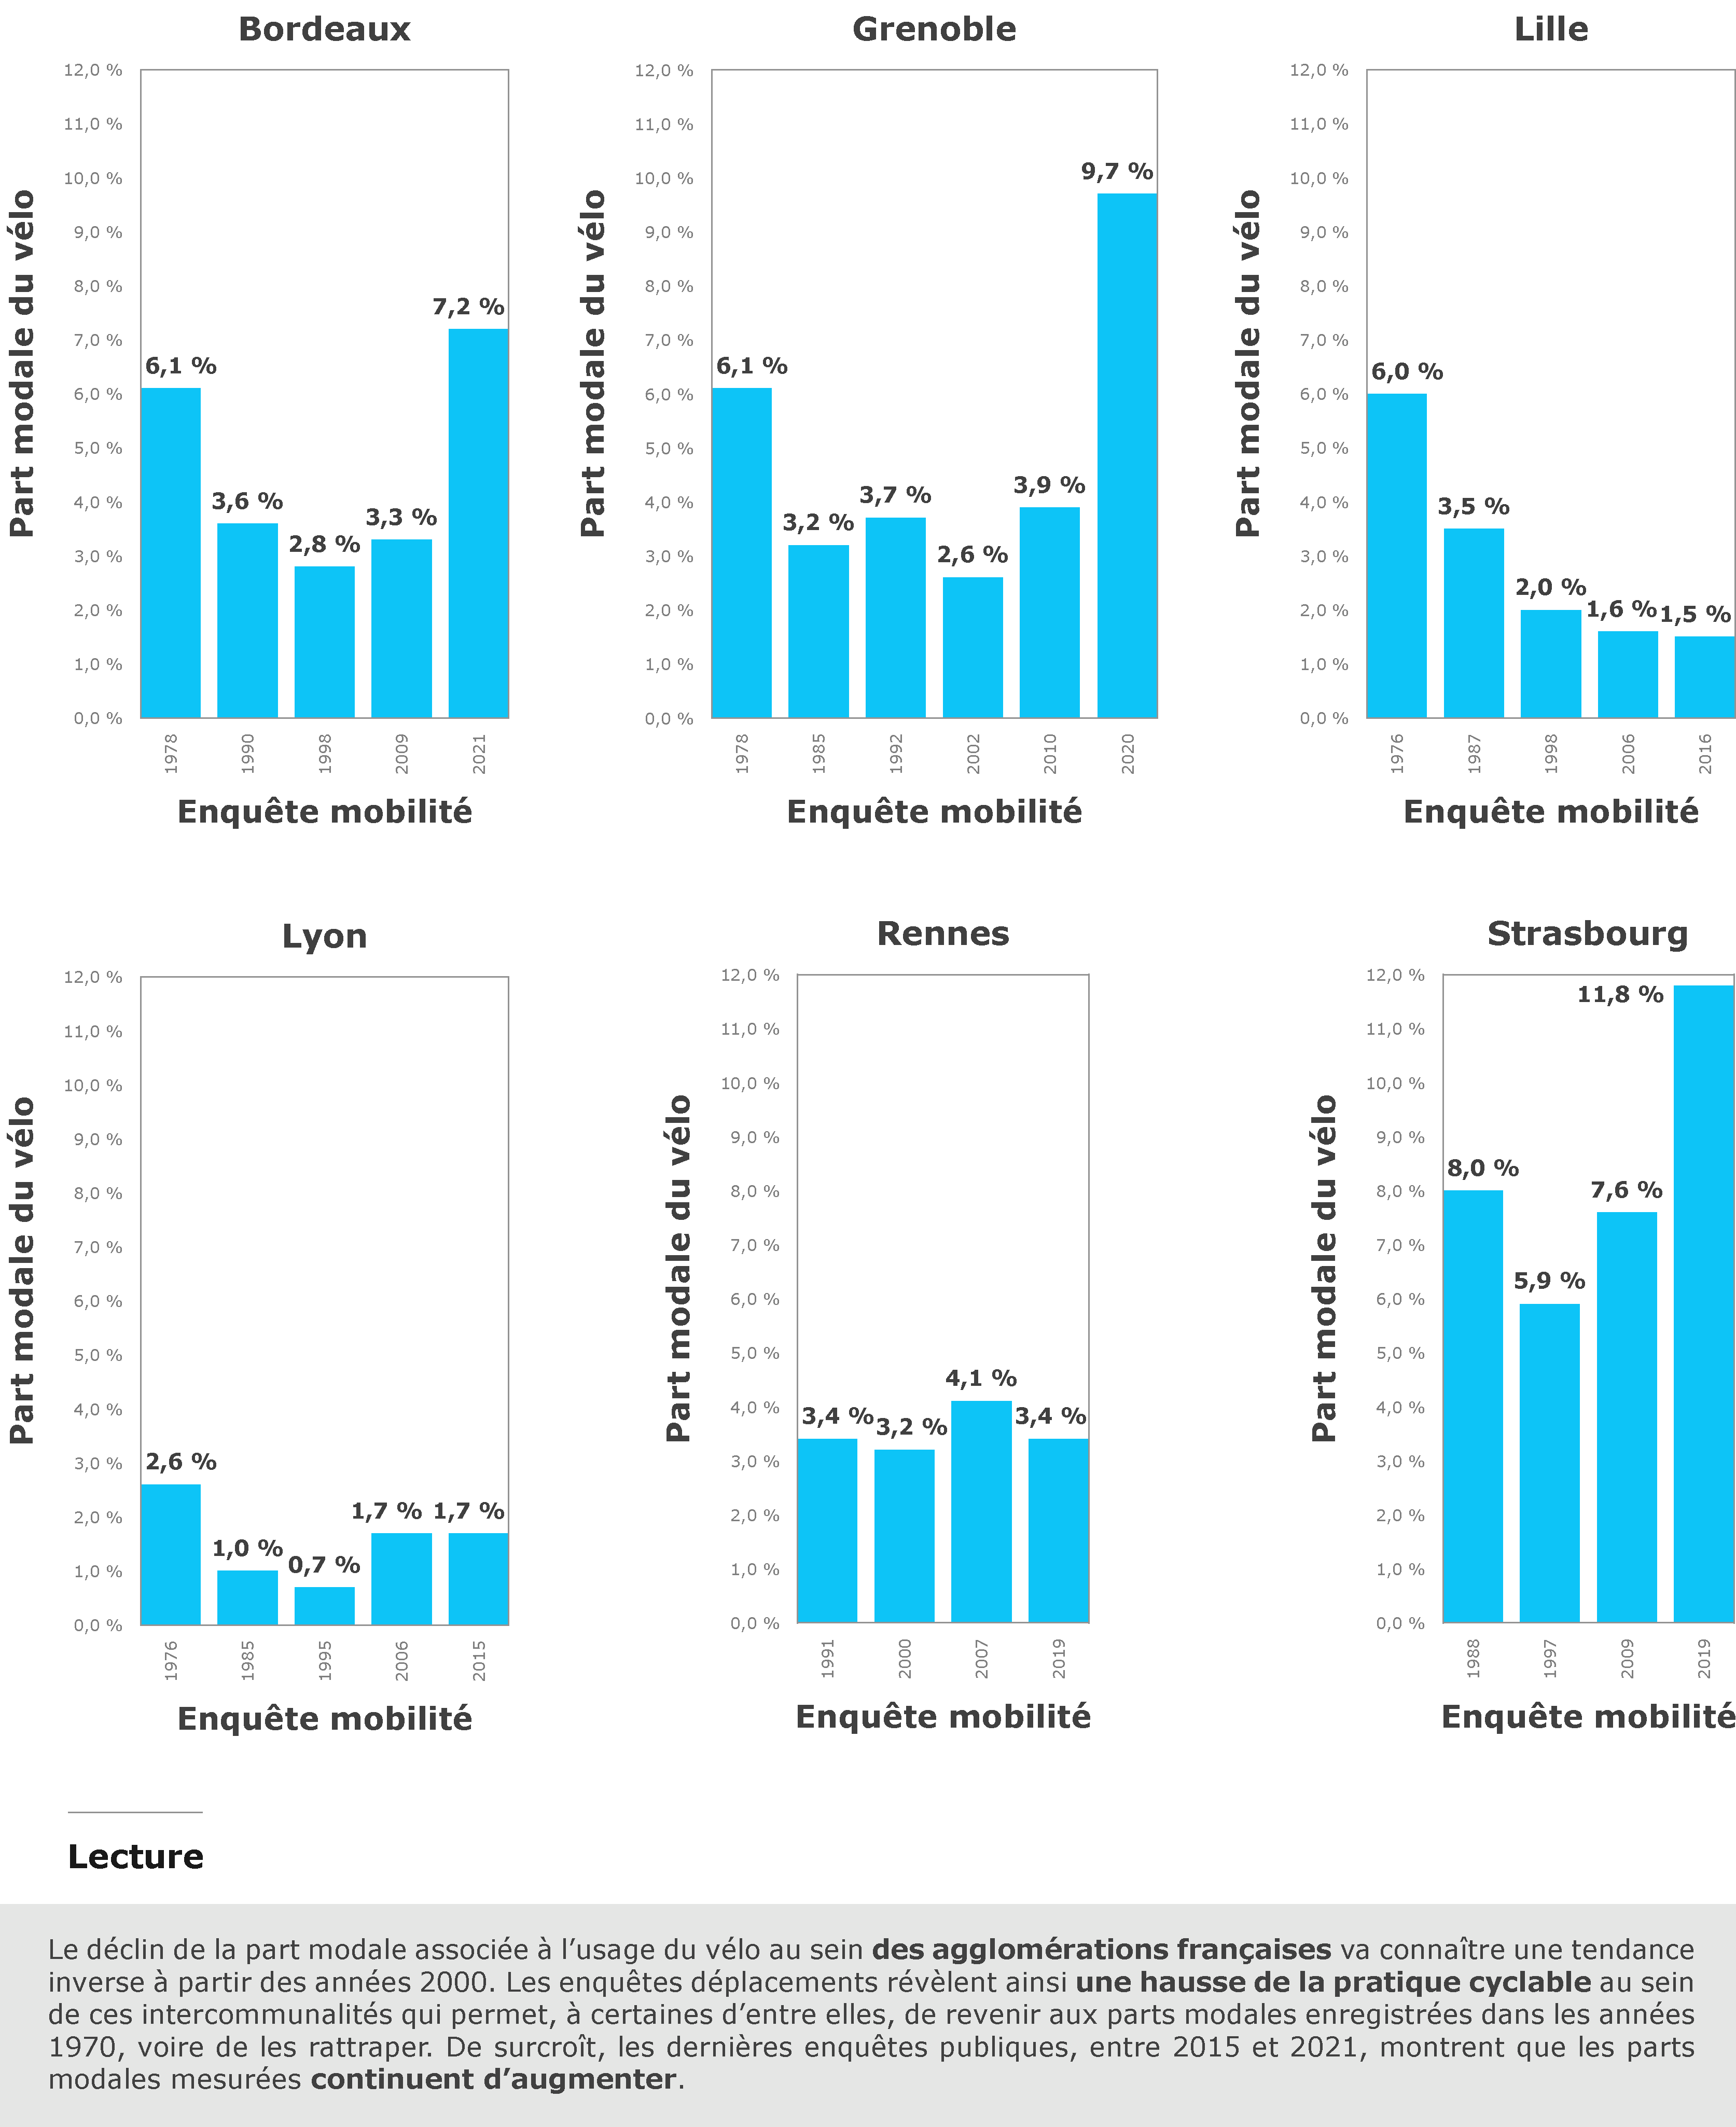
\includegraphics[width=1\columnwidth]{src/Figures/Chap-1/FR_Part_modale_velo_evolution.pdf}}
        \vspace{5pt}
        \begin{flushleft}\scriptsize{
        Note~: les territoires renvoient à leur échelle intercommunale, tandis que les enquêtes mobilité se rapportent au corpus d'\acrfull{EMD} au standard \textsl{Certu} ou certifiée \textsl{Cerema}.
        }\end{flushleft}
        \begin{flushright}\scriptsize{
        Jeux de données~: analyse issue du \textcolor{blue}{\textcite[48]{certu_usagers_2013}}\index{Certu@\textsl{Certu}|pagebf}\index{Cerema@\textsl{Cerema}|pagebf}\index{Jolly, Thomas|pagebf}
        \\
        Adaptation graphique et actualisation~: \textcolor{blue}{Dylan Moinse (2025)}
        }\end{flushright}
    \end{figure}
    
    % Retour en grâce vélo et trottinette
Le \Guillemets{retour en grâce} du vélo dans les territoires français \textcolor{blue}{\autocites[137-168]{heran_retour_2015}[44]{eskenazi_voir_2022}}\index{Héran, Frédéric|pagebf}\index{Eskenazi, Manon|pagebf} s’inscrit dans une dynamique amorcée il y a plus de quarante ans. Ce renouveau marque une seconde période de conquête pour le vélo, longtemps disqualifié dans les mobilités quotidiennes \textcolor{blue}{\autocite[26]{papon_retour_2012}}\index{Papon, Francis|pagebf}, alors que l’usage utilitaire du vélo continue de décliner dans les métropoles françaises, avec une diminution de 50~\% à 75~\% entre 1975 et 1990 \textcolor{blue}{\autocite[48]{certu_usagers_2013}}\index{Certu@\textsl{Certu}|pagebf}\index{Cerema@\textsl{Cerema}|pagebf}\index{Jolly, Thomas|pagebf}. Déjà en 1976, le journal \textsl{Le Monde} pointait une contradiction dans le fait de \Guillemets{moquer} les cyclistes \Guillemets{oublié·e·s}, alors que le parc de vélos, estimé à 17 millions, rivalisait avec le nombre de voitures particulières en possession \textcolor{blue}{\autocite{ambroise-rendu_creation_1976}}\index{Ambroise-Rendu, Marc|pagebf}\index{Le Monde@\textsl{Le Monde}|pagebf}. Les enquêtes de déplacements réalisées à partir des années 2000 mettent l'accent sur une résurgence du vélo parmi les pratiques de mobilité quotidienne (voir l'\hyperref[fig-chap1:evolution-part-modale-velo]{illustration~\ref{fig-chap1:evolution-part-modale-velo}}, page~\pageref{fig-chap1:evolution-part-modale-velo}). L’agglomération lyonnaise voit ainsi la part modale du vélo quadrupler entre 1995 et 2006, tandis que celle de \acrfull{MEL} compense son déclin entre 1998 et 2006 \textcolor{blue}{\autocite[243]{dauncey_french_2012}}\index{Dauncey, Hugh|pagebf}. Ce phénomène s’explique par la montée des préoccupations environnementales, conjuguée aux répercussions des crises économiques et énergétiques successives \textcolor{blue}{\autocite[138]{heran_retour_2015}}\index{Héran, Frédéric|pagebf}, ainsi qu’à la densification des tissus associatifs et à l’évolution des cadres légaux et réglementaires \textcolor{blue}{\autocite[55]{sebban_complementarite_2003}}\index{Sebban, Annie-Claude|pagebf}\index{Motte, Alain|pagebf}. Cette période voit également l’apparition de nouveaux modèles de cycle, tels que le vélo de ville, conçu pour un usage urbain, ou le vélo pliant en aluminium \Marque{Brompton} \textcolor{blue}{\autocite[55]{sebban_complementarite_2003}}\index{Sebban, Annie-Claude|pagebf}\index{Motte, Alain|pagebf}. Mais c'est surtout la grève des transports publics de 1995, très suivie, qui représente un moment décisif dans ce tournant et qui va permettre au vélo de se repositionner comme une alternative crédible. La résurgence du vélo s’accompagne d’une mutation sociologique et spatiale~: alors que le vélo des années 1970 était majoritairement utilisé par des populations captives en périphérie urbaine, les années 1990 voient émerger des usager·ère·s issu·e·s des classes moyennes et supérieures, se déplaçant en milieu urbain\footnote{
    D'après \textcolor{blue}{Frédéric} \textcolor{blue}{\textcite[143]{heran_retour_2015}}\index{Héran, Frédéric|pagebf}, \Guillemets{\textsl{en 1982, le cycliste type était un homme plutôt jeune, sans permis de conduire, issu d'une famille nombreuse, ouvirère ou agricole, souvent immigrée, à revenus modestes et peu ou pas motorisée, circulant en banlieue ou dans une ville de province. Il allait à vélo à l'école ou au travail, en rêvant d'acheter un vélomoteur et, un jour, une voiture. Selon les résultats de l'ENTD 2007-2008, ces usagers sont toujours majoritairement des hommes (à 63~\%), mais désormais surtout des cadres de la fonction publique et des professions libérales, beaucoup plus rarement des ouvriers ou des employés.}}. Par ailleurs, les cyclistes urbain·e·s ont remplacé les \Guillemets{prolétaires de la circulation} \textcolor{blue}{\autocite{ambroise-rendu_creation_1976}}\index{Ambroise-Rendu, Marc|pagebf}, devenant une spécificité française en raison d’investissements presque exclusivement concentrés sur les hypercentres \textcolor{blue}{\autocite[144]{heran_retour_2015}}\index{Héran, Frédéric|pagebf}.
} \textcolor{blue}{\autocite[143]{heran_retour_2015}}\index{Héran, Frédéric|pagebf}.%%Rédigé%%

    % Transition
Bien que la part modale du vélo reste modeste en France~–~à hauteur de 3~\% des déplacements, contre 10~\% en Allemagne et 27~\% aux Pays-Bas~–, cette période est marquée par un élan inédit en faveur du vélo utilitaire \textcolor{blue}{\autocite[222]{dauncey_french_2012}}\index{Dauncey, Hugh|pagebf}. Des initiatives locales comme le \textsl{Plan vélo} de Strasbourg, qui a transformé un réseau cyclable fragmenté en un maillage continu de 483 km en 2006, illustrent cette dynamique. Depuis les années 2010, le vélo est intimement lié aux enjeux environnementaux et sanitaires. Face à la pollution urbaine et à la congestion automobile, il est perçu comme une solution à faible impact écologique, bénéfique pour la santé publique et économique. Les efforts en faveur de son développement traduisent une volonté de promouvoir une véritable \Guillemets{écomobilité} \textcolor{blue}{\autocites[4]{sebban_complementarite_2003}{heran_transition_2018}}\index{Sebban, Annie-Claude|pagebf}\index{Motte, Alain|pagebf}\index{Héran, Frédéric|pagebf}, marquant un retour des \Guillemets{modes oubliés} dans les pratiques de mobilité quotidienne \textcolor{blue}{\autocite[35]{papon_retour_2012}}\index{Papon, Francis|pagebf}. Il aurait également été possible d’évoquer l’histoire conjointe d’autres \Guillemets{objets de glisse urbaine}, tels que le \textsl{skateboard} ou le patin à roulettes\footnote{
    Cette perspective diffère quelque peu pour ces autres véhicules, qui demeurent principalement associés aux loisirs et n’ont pas vocation à répondre à des besoins de mobilité directive ou à partager l’espace de voirie de manière structurée.
}, mais l’objectif ici n’est pas de proposer une analyse exhaustive ni de retracer l’intégralité de l’histoire du cycle. L’intention est plutôt de connecter le développement des cycles aux héritages de l'urbanisme diffus, façonné par l’automobile. Les investissements entrepris pour remettre le vélo sur le devant de la scène se sont accompagnés d'initiatives locales, incluant la mise en place d'aménagements cyclables et l'installation de services de mobilité, tels que les systèmes de \acrshort{VLS} \textcolor{blue}{\autocite[244]{dauncey_french_2012}}\index{Dauncey, Hugh|pagebf}, ainsi que le déploiement de l'électromobilité.%%Rédigé%%

    % 1.2.2.
    \needspace{1\baselineskip} % Réserve de l'espace
\subsection{Élargissement de l’offre par la motorisation électrique et l’introduction de systèmes de véhicules mutualisés
    \label{chap1:velo-micromobilite-innovations}
    }

    % Introduction
Alors que la pratique du vélo connaît une multiplication par 32 entre 1894 et 1934 \textcolor{blue}{\autocite[139]{orselli_usages_2008}}\index{Orselli, Jean|pagebf}, non sans susciter d’importantes difficultés d’acceptation sociale, elle décline ensuite au profit de l’automobile, laquelle fait face à des problématiques similaires d’appropriation. Si une lecture néolibérale des dynamiques urbaines se manifeste clairement à travers l’émergence de services de mobilité en libre-service, d’abord avec station, puis sans station, ces dispositifs traduisent une orientation vers un urbanisme davantage tourné vers l’entrepreneuriat et une redéfinition des rôles traditionnels des pouvoirs publics \textcolor{blue}{\autocites[169]{delaunay_mobilites_2017}{frotey_maxime_2017}}\index{Frotey, Julia|pagebf}\index{Delaunay, Teddy|pagebf}\index{Lesteven, Gaële|pagebf}. Pour autant, le débat se cristallise bel et bien autour du partage de l'espace public. Ces controverses rappellent les luttes historiques pour le partage de la voirie, déjà observées lors de l’arrivée successive de la traction hippomobile, du tramway, puis de l’automobile. Chaque nouvelle technologie de mobilité, en transformant les usages et les rapports sociaux dans l’espace urbain, réactive des dynamiques conflictuelles liées à la cohabitation et à la répartition des ressources spatiales\footnote{
    Aussi, nous pouvons également évoquer les querelles suscitées par le développement du tramway durant son âge d’or, s’étendant de la fin du XIX\textsuperscript{e} siècle à l’entre-deux-guerres \textcolor{blue}{\autocite[281]{flonneau_concurrence_2007}}\index{Flonneau, Mathieu|pagebf}. Ces controverses ont refait surface lors de son retour progressif au cours des années 2000, accompagné de craintes tant populaires que politiques. En effet, le tramway était perçu comme un moyen de transport désuet, appartenant à une autre époque \textcolor{blue}{\autocite[110]{gardon__2014}}\index{Flonneau, Mathieu|pagebf}. Toutefois, ces représentations négatives se sont estompées au profit d’une image renouvelée et moderne, grâce à l’intégration d’innovations techniques telles que les planchers bas et ultra-bas ou encore les systèmes d’alimentation par le sol. Ce renouveau du tramway, loin d’être un processus consensuel, a néanmoins généré des tensions, notamment vis-à-vis de l’automobile, qu’il concurrence directement. Le rapport de force qui en découle a conduit à une reconfiguration des tracés des projets de tramway, souvent conçus pour minimiser les impacts sur la voirie et les espaces de stationnement automobile. Dans certains cas, cette réconciliation spatiale s’est traduite par l’aménagement de sections de tramway en souterrain, permettant ainsi de préserver les voies de circulation automobile \textcolor{blue}{\autocite[10]{richer_tramways_2012}}\index{Richer, Cyprien|pagebf}\index{Hasiak, Sophie|pagebf}. Par ailleurs, le tramway a également été accusé de concurrencer d’autres systèmes de transport public préexistants, notamment les réseaux ferroviaires régionaux \textcolor{blue}{\autocite[36]{cete_nord_picardie_evaluer_2013}}.
}. Toutefois, le \Guillemets{retour} du vélo en milieu urbain s’accompagne, ces dernières décennies, de l’apparition de nouvelles catégories de cycles. Cette diversification de l'offre en \Guillemets{altermobilités} \textcolor{blue}{\autocite[91-92]{vincent-geslin__2012}}\index{Vincent-Geslin, Stéphanie|pagebf}, est marquée par l’émergence de l’électromobilité, illustrée tout d’abord par le redéploiement du \acrshort{VAE}, suivi par le développement de la \acrshort{TEP}, ainsi que par de nouvelles modalités d’acquisition, telles que la mise à disposition de flottes partagées de vélos et de trottinettes. Ainsi, comme nous l’avons observé, ces véhicules jouissent de cycles d’innovations, qu’elles soient techniques, servicielles ou organisationnelles. En adoptant une perspective historique sur l’évolution de la place occupée par ces véhicules, il apparaît que, malgré une perception parfois jugée désuète ou limitée à un usage ludique pour enfants, un siècle d’innovations appliquées à ces objets a permis leur réintroduction sous des formes modernisées, dans un contexte opportun. En jouant sur un registre mêlant nostalgie et modernité, ces véhicules se sont progressivement affirmés comme des modes de déplacement fiables, tirant parti à la fois de l’électrification, qui étend leur facilité et leur portée d’usage, et des systèmes de partage, qui accroissent leur accessibilité et leur visibilité dans l’espace public. Ce phénomène peut être interprété à travers la notion de \Guillemets{rétro-innovation}, issue du champ du \textsl{marketing} et de la communication, définie comme la réinvention d’un produit ou d’un domaine d’activité grâce à des innovations technologiques, dans l’objectif de lui conférer un nouvel usage tout en établissant un lien avec le passé \textcolor{blue}{\autocite{barthelot_retro-innovation_2018}}\index{Barthelot, Bertrand|pagebf}. Parmi les trois catégories constitutives de la rétro-innovation, les cycles électrifiés et les dispositifs partagés s’inscrivent dans la tendance dite de l’\textsl{inn-old-vation}, laquelle repose sur l’intégration d’innovations technologiques visant à adapter un produit à des besoins préexistants \textcolor{blue}{\autocite{lamy_retro-innovation_2016}}\index{Lamy, Alexia|pagebf}. Cependant, comme nous le verrons, la difficulté majeure réside dans l’introduction de ces innovations, qu’elles soient techniques ou sociales, un défi qui accompagne le vélo depuis les prémices de son histoire moderne \textcolor{blue}{\autocite[33]{jouenne_quest-ce_2022}}\index{Jouenne, Noël|pagebf}.%%Rédigé%%

    % 1.2.2.1.
    \needspace{1\baselineskip} % Réserve de l'espace
\subsubsection*{Contribution de l'électromobilité à la diversification du vélo et de la micro-mobilité
    \label{chap1:velo-micromobilite-innovations-electromobilite}
    }

    % Introduction
Au développement du vélo et du vélo pliant se sont ajoutés de nouveaux modes de déplacement à propulsion électrique, élargissant la famille des cycles \textcolor{blue}{\autocite[5]{lopez-escolano_mobilites_2019}}\index{López-Escolano, Carlos|pagebf}\index{Campos, Ángel Pueyo|pagebf}. Parmi eux, le \acrfull{VAE}, qu’il soit pliant ou non, la \acrfull{TEP}, ainsi qu’une variété d’engins de déplacement regroupés sous l’appellation de \Guillemets{micro-mobilité} (voir l'\hyperref[fig-chap1:ecosysteme-micromobilite]{illustration~\ref{fig-chap1:ecosysteme-micromobilite}}, page~\pageref{fig-chap1:ecosysteme-micromobilite}), tels que le monoroue (ou gyroroue), l’\textsl{hoverboard} ou encore le gyropode (\textsl{segway}). La liste des \acrfull{NVEI} ne cesse de s’allonger, illustrant une diversification modale permise notamment par la réduction des coûts de fabrication, la miniaturisation des composants et les gains d’efficacité des batteries électriques, qui en facilitent la portabilité\footnote{
    Les années 1990 ont marqué un tournant décisif pour les \textsl{pedelecs}, lorsque plusieurs avancées techniques ont convergé pour en accroître la praticité et l’attractivité. L’introduction et la commercialisation de batteries plus légères et plus performantes, telles que la batterie \acrfull{NiCd} et, ultérieurement, la batterie \acrfull{NiMH}, ont joué un rôle stratégique dans leur évolution. Ces nouvelles batteries offrent un rapport énergie/poids nettement supérieur à celui de leurs prédécesseurs, rendant le vélo électrique à la fois plus léger, maniable et doté d’une meilleure autonomie. L’introduction de l'accumulateur \acrfull{Li-ion}, comparativement aux batteries antérieures, a marqué une étape supplémentaire. Ce type de batterie électrique, de taille équivalente, présente une capacité énergétique supérieure de 32~\% et un poids réduit de 25~\%. Par ailleurs, la batterie \acrshort{Li-ion} présente une décharge à courant élevé, l’absence d’effet mémoire et la possibilité de recharger la batterie à tout moment.
} \textcolor{blue}{\autocites[430]{bertoluzzo_development_2011}[2]{schultz_micromobility_2019}[430]{pages_nouveaux_2021}}\index{Schultz, Stéphane|pagebf}\index{Grisot, Sylvain|pagebf}\index{Bertoluzzo, Manuele|pagebf}\index{Buja, Giuseppe|pagebf}\index{Pages, Thibaud|pagebf}\index{Lammoglia, Adrien|pagebf}\index{Josselin, Didier|pagebf}.%%Rédigé%%

    % Figure écosystème du vélo et micro-mobilité
    \begin{figure}[h!]\vspace*{4pt}
        \caption{Écosystème de la \Guillemets{mobilité individuelle et locale}, à propulsion humaine, à assistance ou motorisée.}
        \label{fig-chap1:ecosysteme-micromobilite}
        \centerline{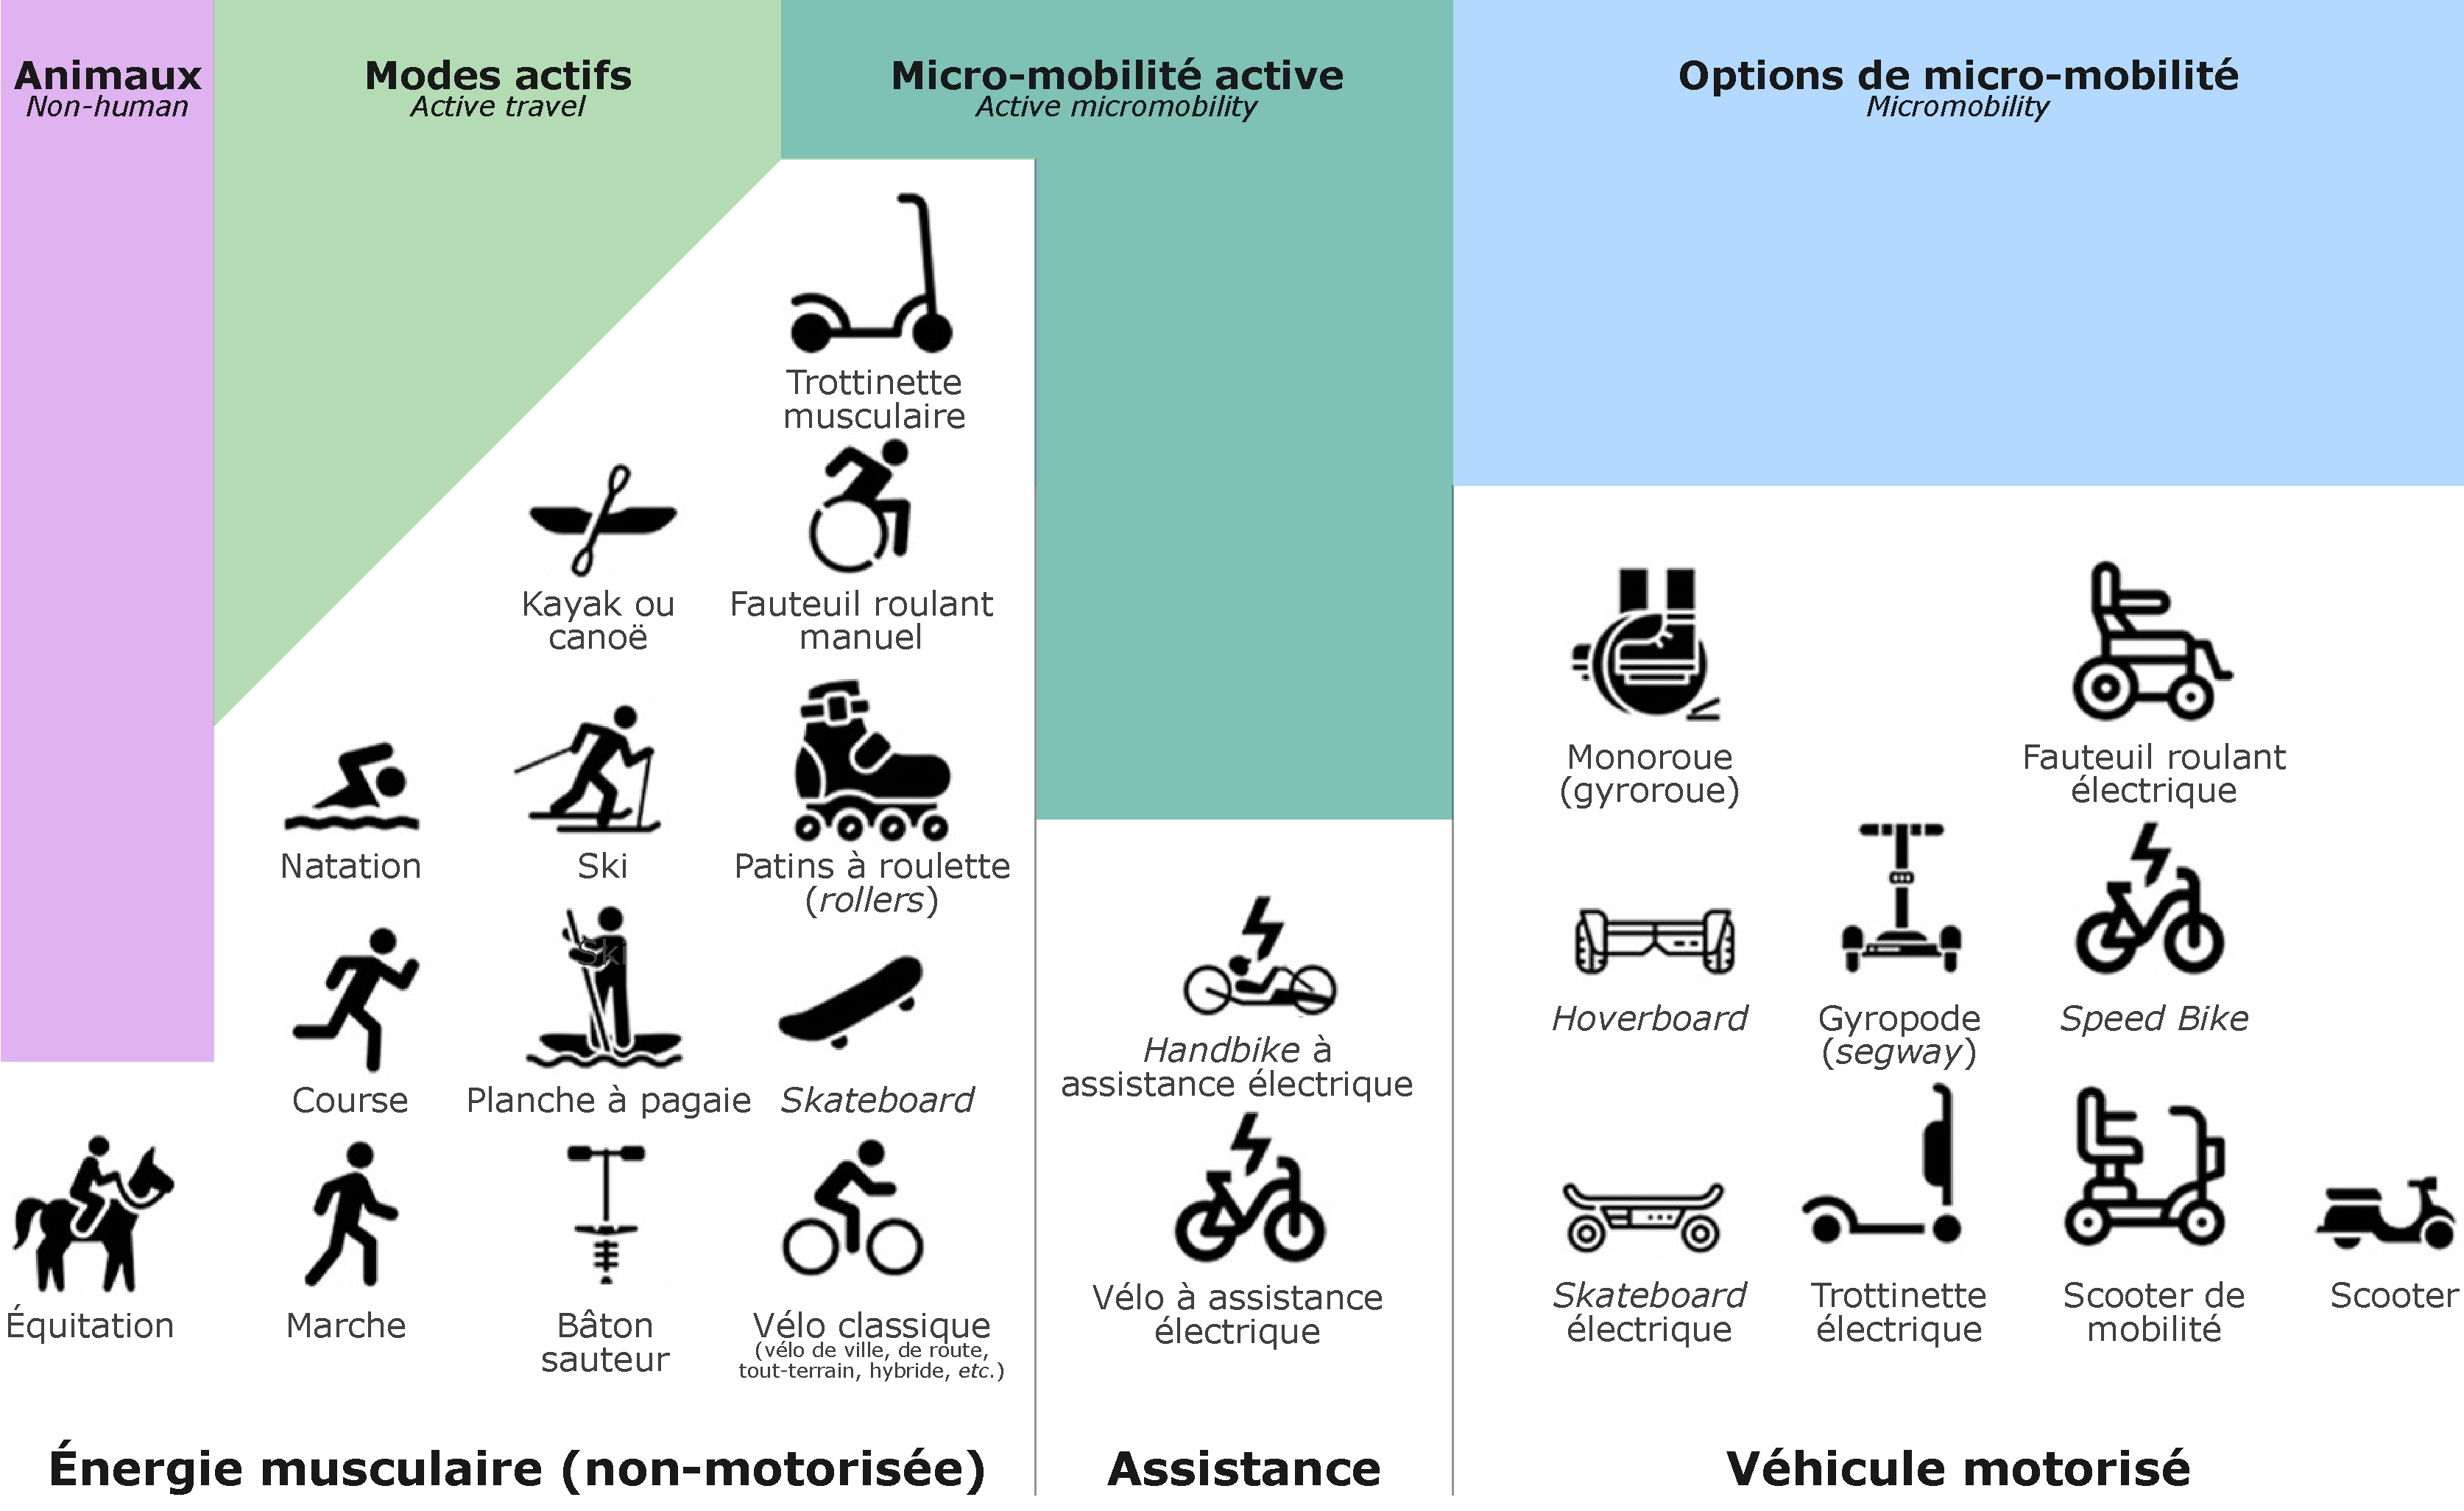
\includegraphics[width=1\columnwidth]{src/Figures/Chap-1/FR_Ecosysteme_micromobilite.pdf}}
        \vspace{5pt}
        \begin{flushright}\scriptsize{
        Source~: \textcolor{blue}{\textcite[155]{cook_more_2022}}\index{Cook, Simon|pagebf}\index{Stevenson, Lorna|pagebf}\index{Aldred, Rachel|pagebf}\index{Kendall, Matt|pagebf}\index{Cohen, Tom|pagebf}
        \\
        Adaptation graphique~: \textcolor{blue}{Dylan Moinse (2024)}
        }\end{flushright}
    \end{figure}

    % Histoire contemporaine VAE
En 1993, le fabricant japonais de moto \Marque{Yamaha Motor Company} a introduit le premier vélo électrique de série, à succès commercial, doté d’une fonction d’assistance au pédalage (\textsl{Power Assist System}) et alimenté par d'une batterie amovible \acrshort{NiMH} \textcolor{blue}{\autocite[430]{bertoluzzo_development_2011}}\index{Bertoluzzo, Manuele|pagebf}\index{Buja, Giuseppe|pagebf}. Ce vélo offre des avantages notables par rapport à la batterie traditionnelle au plomb, en proposant une batterie plus légère, moins sensible aux variations de température ambiante et avec un cycle de vie plus long. Le système d'assistance au pédalage a non seulement permis de prolonger la durée de vie de la batterie, mais aussi de rendre l'expérience de l'utilisateur·rice plus intuitive. En raison de ces qualités, \textcolor{blue}{Noël} \textcolor{blue}{\textcite[25]{jouenne_quest-ce_2022}}\index{Jouenne, Noël|pagebf} qualifie le \acrshort{VAE} de \Guillemets{vélo à assistance électro-mécanique} dans son \acrfull{HDR} portant sur l’ethnologie du vélo comme objet technique et social, pour insister sur le mix énergétique requis pour se déplacer. À partir de 2003, le vélo électrique profite du développement et de la commercialisation de la batterie \acrshort{Li-ion} \textcolor{blue}{\autocite[6]{hung_review_2020}}\index{Hung, Nguyen Ba|pagebf}\index{Lim, Ocktaeck|pagebf}. En France, les ventes de \acrshort{VAE} ont connu une croissance spectaculaire, passant de 37~000 unités vendues en 2011 à 338~000 en 2018, atteignant 738~000 en 2022, avant une légère baisse à 671~000 produits en 2023. Ces chiffres représentent 43~\% des ventes totales de véhicules électriques en 2023 \textcolor{blue}{\autocite{union_sport__cycle_chiffres_2024}}\index{Union Sport \& Cycle@\textsl{Union Sport \& Cycle}|pagebf}. Parallèlement au \acrshort{VAE}, des formes nouvelles du vélo comme le vélo-cargo et le triporteur ont élargi les possibilités d’utilisation du vélo électrique. Ces modèles facilitent, outre les déplacements sur de longues distances ou pour les personnes âgées ou à mobilité réduite, le transport de personnes et d’objets lourds. Ils ouvrent ainsi de nouvelles perspectives pour les déplacements familiaux ou sous forme de vélotaxis, le secteur de la logistique urbaine et l'autoentrepreneuriat. Selon \textcolor{blue}{\textcite[24]{mason_global_2015}}\index{Mason, Jacob|pagebf}\index{Fulton, Lew|pagebf}\index{McDonald, Zane|pagebf}, la part modale du vélo, stimulée par la popularité croissante du \acrshort{VAE}, pourrait atteindre 17~\% en 2030 et 22~\% en 2050 parmi les pays de l'\acrfull{OCDE}.%%Rédigé%%

    % Histoire contemporaine TEP + Transition
Concomitamment à l’essor du \acrshort{VAE}, la trottinette revient sur le devant de la scène, d’abord comme jouet, puis progressivement adoptée par les adolescent·e·s\footnote{
    La diffusion de la trottinette moderne est favorisée par une innovation technique majeure qui la rend plus légère, plus résistante et plus maniable grâce à l’emploi de l’aluminium, un matériau qui permet également de la rendre pliable \textcolor{blue}{\autocite{arte_histoire_2014}}. En 1996, l’homme d’affaires suisse \textcolor{blue}{Wim Ouboter} joue un rôle déterminant dans l’évolution de la trottinette. Il fonde sa propre entreprise, \Marque{Micro Mobility Systems}, et conçoit dès 1999 des \Guillemets{micro-trottinettes}, connues sous le nom de \textsl{micro-scooters}, en combinant l’esthétique de la trottinette avec des roues inspirées du \textit{skateboard} \textcolor{blue}{\autocite{les_numeriques_futur_2015}}\index{Les Numériques@\textsl{Les Numériques}|pagebf}. Rapidement, ce modèle, commercialisé sous la marque \Marque{Razor}, devient un phénomène mondial, atteignant un million d’unités vendues en 2000 avant que l’engouement ne s’atténue. Malgré ce déclin, la trottinette conserve son statut de jouet destiné principalement aux enfants. Aux États-Unis, elle \Guillemets{envahit les cul-de-sacs des zones résidentielles}, et la \textsl{Toy Association} désigne ce modèle comme \Guillemets{jouet de l’année} en 2000 \textcolor{blue}{\autocite{bloomberg_citylab_man_2018}}. Cependant, cet engouement s’essouffle rapidement \textcolor{blue}{\autocite[25]{university_of_st_gallen_micro_2011}}\index{University of St. Gallen@\textsl{University of St. Gallen}|pagebf}. Parallèlement, la trottinette évolue en se redéployant dans un cadre différent. Un changement d’usage et de clientèle s’opère~: la trottinette renforcée devient un support pour une nouvelle discipline sportive, le \textsl{freestyle}, inspirée du BMX (\textsl{bicycle motocross}) et du \textit{skateboard}. Ce sport, qui consiste à réaliser des figures acrobatiques (\textsl{tricks}), attire une nouvelle génération d’usager·ère·s, les \textsl{trottiriders} \textcolor{blue}{\autocite{micro-mobility_innovations_2018}}\index{Micro-mobility@\textsl{Micro-mobility}|pagebf}. Ainsi, la trottinette cesse progressivement d’être perçue comme un simple jouet pour devenir un équipement prisé par les adolescent·e·s et les jeunes adultes, séduit·e·s par les sports de glisse et par la culture urbaine \textcolor{blue}{\autocite{ma_trott_histoire_2020}}.
} avant de connaître une transformation grâce à un \textsl{design} modernisé et l’intégration d’une batterie électrique. L’homme considéré comme \Guillemets{le pionnier de la révolution de la trottinette}, \textcolor{blue}{Wim Ouboter}, amorce cette transformation à partir de son expérience personnelle\footnote{
    \textcolor{blue}{Wim Ouboter} relate que son intérêt pour la trottinette trouve ses racines dans son expérience personnelle. Lorsqu’il était enfant, lui et sa sœur utilisaient d’anciennes trottinettes, cette dernière étant dans l’incapacité de pratiquer le vélo ou le ski en raison d’un handicap physique. Cependant, c’est à l’âge de 30 ans que survient la véritable révélation. D'après le récit exposé, l'entrepreneur suisse aurait réalisé alors que son restaurant de saucisses préféré, situé à Zurich, se trouverait à une distance trop importante pour y aller à pied, mais pas assez éloigné pour justifier l’utilisation d’un vélo ou d’une voiture \textcolor{blue}{\autocite{ma_trott_histoire_2020}}.
} \textcolor{blue}{\autocite{ma_trott_histoire_2020}}\index{Ma Trott'@\textsl{Ma Trott'}|pagebf}. La trottinette est réhabilitée avec la création de la \Marque{Micro}, conçue pour les déplacements qualifiés de \Guillemets{micro-distance}, situés entre des trajets trop longs pour marcher et trop courts pour avoir recours à une voiture ou à un vélo \textcolor{blue}{\autocite{oconnell_travel_2002}}\index{O'Connel, Dee|pagebf}. Dans le prolongement de l’électrification de la mobilité urbaine en 2003, l’entrepreneur suisse élargit sa gamme en développant des modèles électriques, toujours en visant une clientèle adulte \textcolor{blue}{\autocite{ma_trott_histoire_2020}}\index{Ma Trott'@\textsl{Ma Trott'}|pagebf}. Mais c’est véritablement le lancement de la trottinette \Marque{Xiaomi Mi Electric Scooter} (M365) en 2016, d'abord en Chine, qui bouscule le marché. Commercialisée en Europe en 2018, la \acrshort{TEP} s’est imposée comme un succès mondial grâce à son coût abordable et à l'ergonomie qu'elle propose. Adoptée massivement pour un usage personnel, elle sert également de modèle de référence pour une multitude de flottes de trottinettes en libre-service. En France, la popularité de la \acrshort{TEP} ne se fait pas attendre~: selon le baromètre de la \acrfull{FP2M}, les ventes démarrent à 233~000 unités en 2018, s'élèvent à 478~800 unités l'année qui suit, pour atteindre 678~000 unités en 2023 \textcolor{blue}{\autocites[1]{fp2m_barometre_2021}[1]{fp2m_ventes_2023}}\index{FP2M@\textsl{FP2M}|pagebf}. Ces chiffres surpassent désormais les ventes de \acrshort{VAE}, pourtant également en expansion. L’exemple de la trottinette, qu’elle fonctionne à propulsion humaine ou électrique, et celui du \acrshort{VAE}, pliant ou classique, illustrent parfaitement la diversification des modes de déplacement en milieu urbain, en se déclinant sous des formes accessibles à l'achat et en location.%%Rédigé%%

    % 1.2.2.2.
    \needspace{1\baselineskip} % Réserve de l'espace
\subsubsection*{L'économie du partage au service de la mobilité partagée
    \label{chap1:velo-micromobilite-innovations-partage}
    }

    % Libre-service avec station - histoire 1
La genèse des \acrshort{VLS} s’inscrit dans l’histoire des mouvements sociaux à l’origine du retour du vélo en ville \textcolor{blue}{\autocite[23]{hure_mobilites_2019}}\index{Huré, Maxime|pagebf}. L’idée d’un \Guillemets{vélo intelligent} (\textsl{smart bike}) partagé dans l’espace public, accessible à tou·te·s sans nécessité d’acquisition personnelle, trouve ses premières applications en 1965 grâce à un collectif anarchiste néerlandais, \textsl{Provo}. Dans le cadre de leur cinquième \Guillemets{provocation} (\textsl{Witte Fietsenplan}) et à l'approche des élections municipales de 1966, ce mouvement contestataire et libertaire met alors à disposition des Amstellodamois·e·s une cinquantaine de vélos peints en blanc, déposés librement dans les rues, dans le but de libérer la ville de la congestion urbaine\footnote{
    Le groupe \textsl{Provo} prône une initiative municipale visant à mettre à disposition de la population 10~000 bicyclettes gratuites, autogérées par un système participatif. En signe de protestation contre le refus de leur projet par la municipalité, le collectif inscrit sur la liste électorale remet en circulation environ une centaine de vélos abandonnés, en les réparant et en les peignant en blanc \textcolor{blue}{\autocite[29]{hure_mobilites_2019}}\index{Huré, Maxime|pagebf}.
} \textcolor{blue}{\autocites[6]{smart_provo_2012}{demain_la_ville_doit-velib_2018}}\index{Smart, Alan|pagebf}\index{Demain La Ville@\textsl{Demain La Ville}|pagebf}. Bien que pionnier, ce moyen d'action reste illégal selon les autorités publiques, donnant néanmoins naissance à la première génération de \acrshort{VLS}, basée sur un système gratuit \textcolor{blue}{\autocite[160]{shaheen_bikesharing_2010}}\index{Shaheen, Susan~A.|pagebf}\index{Guzman, Stacey|pagebf}\index{Zhang, Hua|pagebf}. La Rochelle est souvent reconnue comme la première ville à avoir institutionnalisé un tel dispositif en 1976 avec ses \textsl{vélos municipaux}, également appelés \textsl{Vélos Jaunes}, une flotte de 350 vélos répartis sur trois points de location\footnote{
    L'expérience très visible du dispositif municipal rochelais pose la question des transformations de l'action publique urbaine en matière de mobilité, jusqu'alors fortement dépendantes des services étatiques en glissant d'un dirigisme étatique à un État régulateur qui reste le premier financeur de ce projet. Avec ses 300 \acrshort{VLS}, le maire de l'époque, \textcolor{blue}{Michel Crépeau}, souhaite \Guillemets{banaliser} l'usage du vélo en ville. Cette politique met en place un périmètre d'accès, limité à l'intérieur de l'enceinte de l'ancienne forteresse, et d'horaires, de 8 heures à 20 heures, la régulation du système étant dépendante de la participation citoyenne des habitant·e·s \textcolor{blue}{\autocite[31]{hure_mobilites_2019}}\index{Huré, Maxime|pagebf}. Un tel projet, inauguré six mois avant les élections municipales, permet au maire de façonner une notoriété internationale et de légitimer une nouvelle politique urbaine de réhabilitation du centre-ville, construisant déjà une première forme de marketing politique et territorial au travers de ces services de mobilité \textcolor{blue}{\autocite[31]{hure_mobilites_2019}}\index{Huré, Maxime|pagebf}. L’année suivante, un second parc de \acrshort{VLS} gratuits, composé de 100 unités, est mis en place grâce à un financement privé reposant sur un modèle de publicité. Cette initiative marque un tournant, puisque le recours à la publicité s’impose progressivement comme une modalité centrale de financement des systèmes \acrshort{VLS} \textcolor{blue}{\autocite[32-35]{fleury_mobilites_2022}}\index{Huré, Maxime|pagebf}\index{Fleury, Antoine|pagebf}\index{Frétigny, Jean-Baptiste|pagebf}\index{Kanellopoulou, Dimitra|pagebf}.
}. Ce modèle inspire d’autres initiatives, à l’instar de celle portée à Cambridge en 1993, et contribue à stabiliser l’architecture marchande de la mobilité partagée telle qu’elle est encore pratiquée aujourd’hui. Finalement, les mécanismes et les valeurs symboliques du \acrshort{VLS} s’inspirent largement de celui du chariot de supermarché, comme le souligne \textcolor{blue}{Maxime} \textcolor{blue}{Maxime} \textcolor{blue}{\textcite[40]{hure_mobilites_2019}}\index{Huré, Maxime|pagebf}. Copenhague marque une étape décisive entre 1989 et 1995 avec la mise en place de \textsl{Bycyklen}, un système exploitant le mécanisme de dépôt de monnaie (\textsl{coin-deposit}) et de supports à vélo. Ce système, considéré comme la deuxième génération de \acrshort{VLS}, est adopté en Europe et aux États-Unis, mais les problèmes de vol liés à l’anonymat des usager·ère·s persistent\footnote{
    Une alternative notable au modèle classique de \acrshort{VLS} est représentée par le service \textsl{Call a Bike}, déployé dans plusieurs villes allemandes, à commencer par Munich en 2000. Ce système repose sur un principe différent~: le vélo, verrouillé dans l’espace public à l’aide d’un cadenas, peut être emprunté et déposé librement. L’accès au vélo nécessite de contacter un service dédié, permettant d’obtenir le code du cadenas moyennant paiement. Ce système propose deux modes de fonctionnement~: \textsl{Call a Bike FLEX}, sans station, et \textsl{Call a bike FIX}, en station \textcolor{blue}{\autocite[18]{6t-bureau_de_recherche_etude_2018}}. À l’époque, la \textsl{Deutsche Bahn} envisageait de déployer ce système dans une centaine de gares du réseau express d'Intercités, afin de favoriser l’intermodalité.
} \textcolor{blue}{\autocite[160]{shaheen_bikesharing_2010}}\index{Shaheen, Susan~A.|pagebf}\index{Guzman, Stacey|pagebf}\index{Zhang, Hua|pagebf}. La troisième génération, incarnée par le \textsl{Vélo à la carte} de Rennes en 1998, introduit des technologies d’identification et de réservation. Ce système informatisé repose sur des kiosques, des cartes personnelles et, ultérieurement, des téléphones portables, permettant un \textsl{check-in} et un \textsl{check-out} du vélo \textcolor{blue}{\autocite[8]{nlc_micromobility_2019}}\index{NLC@\textsl{NLC}|pagebf}.%%Rédigé%%

   % Figure carte VLS France
    \begin{carte}[h!]\vspace*{4pt}
        \caption{Localisation et évolution des services de vélo en libre-service avec station en France, en 2018.}
        \label{fig-chap1:carte-vls-france}
        \centerline{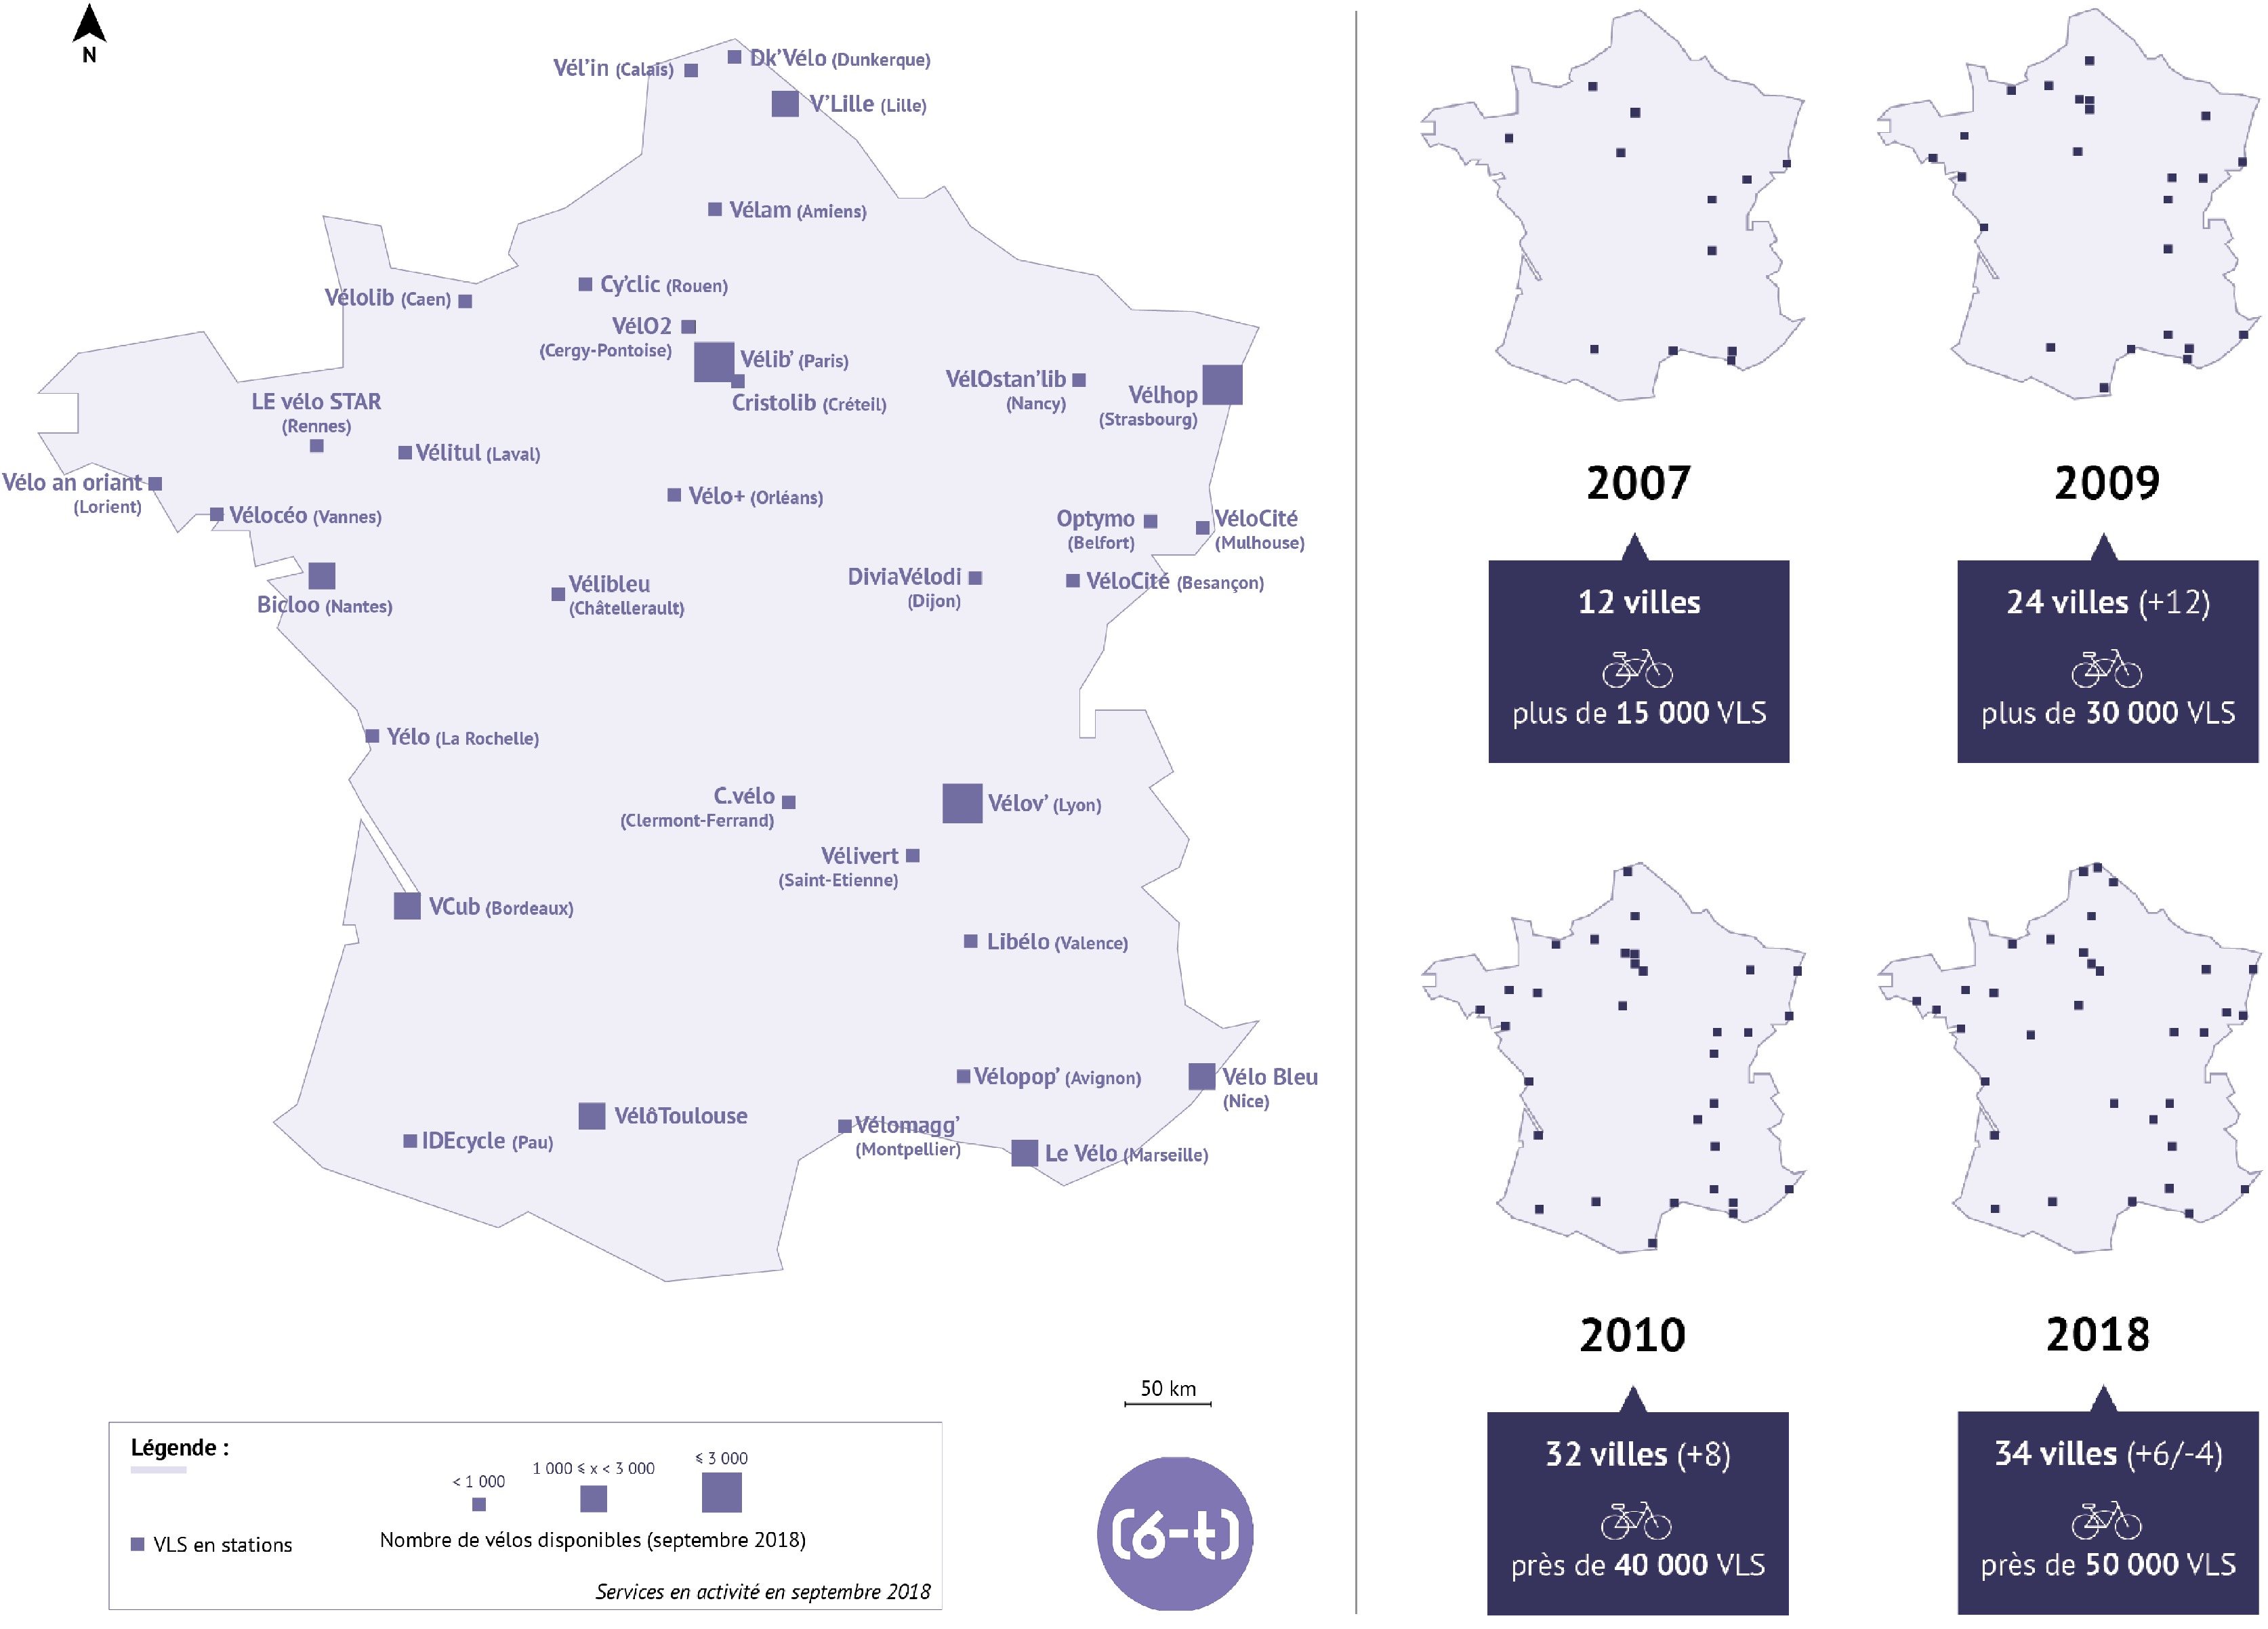
\includegraphics[width=1\columnwidth]{src/Figures/Chap-1/FR_Carte_VLS_France.jpg}}
        \vspace{5pt}
        \begin{flushright}\scriptsize{
        Source~: \textcolor{blue}{\textcite{6t-bureau_de_recherche_lechappee_2018}}\index{Bureau de recherche 6t@\textsl{Bureau de recherche 6t}|pagebf}
        }\end{flushright}
    \end{carte}

    % Libre-service avec station - histoire 2
Ces innovations, associées à un modèle de tarification basé sur des intervalles temporels, deviennent le standard international des systèmes de \acrshort{VLS} \textcolor{blue}{\autocite[162]{shaheen_bikesharing_2010}}\index{Shaheen, Susan~A.|pagebf}\index{Guzman, Stacey|pagebf}\index{Zhang, Hua|pagebf}. C’est toutefois Lyon, avec \textsl{Vélo'v} en 2005, et Paris, avec \textsl{Vélib'} en 2007, qui popularisent ce modèle dans le monde. Ces services deviennent les références en matière de \acrshort{VLS}, permettant à la France de se positionner au premier rang dans ce domaine~: en 2010, le pays compte 24 systèmes de \acrshort{VLS}, avec une flotte totale composée de 36~000 vélos et de 3~000 stations \textcolor{blue}{\autocite[161]{shaheen_bikesharing_2010}}\index{Shaheen, Susan~A.|pagebf}\index{Guzman, Stacey|pagebf}\index{Zhang, Hua|pagebf}, atteignant 34 agglomérations en 2018 (voir la \hyperref[fig-chap1:carte-vls-france]{carte~\ref{fig-chap1:carte-vls-france}}, page~\pageref{fig-chap1:carte-vls-france}). C'est au tournant de cette décennie que les expériences de systèmes de \acrshort{VLS} vont faire apparaître un modèle de gestion dominant~: celui du \acrfull{PPP} \textcolor{blue}{\autocite[5]{hure_entre_2014}}\index{Huré, Maxime|pagebf}. Plus récemment, une quatrième génération émerge, intégrant des \acrshort{VAE} en libre-service, des mécanismes de verrouillage optimisés, des interfaces tactiles et une interconnexion avec les systèmes de transport public \textcolor{blue}{\autocite[162]{shaheen_bikesharing_2010}}\index{Shaheen, Susan~A.|pagebf}\index{Guzman, Stacey|pagebf}\index{Zhang, Hua|pagebf}. Notons que si ces initiatives sont majoritairement le fruit de projets locaux ou intercommunaux portés principalement par les plus grandes agglomérations \textcolor{blue}{\autocites[18]{fishman_bike_2013}[6]{ricci_bike_2015}}\index{Fishman, Elliot|pagebf}\index{Washington, Simon|pagebf}\index{Haworth, Narelle|pagebf}\index{Ricci, Miriam|pagebf}, leur déploiement reste encore marginal à l’échelle régionale ou nationale\footnote{
    Parmi ces exceptions, nous ne pouvons nous empêcher de citer le système néerlandais \textsl{OV-fiets}, littéralement traduit par \textsl{vélos de transport public}, intégré au réseau ferroviaire national. Créé en 2004 par une association, ce système de \acrshort{VLS} a été repris, à partir de 2008, par la compagnie ferroviaire nationale des Pays-Bas, la \acrfull{NS} \textcolor{blue}{\autocites[151]{ploeger_sociotechnical_2020}[157]{waes_why_2020}}\index{Ploeger, Jan|pagebf}\index{Oldenziel, Ruth|pagebf}\index{Waes, Arnoud van|pagebf}\index{Farla, Jacco|pagebf}\index{Raven, Rob|pagebf}. Aujourd’hui, ce service de mobilité couvre 300 stations situées à proximité des gares et des arrêts de métro, avec une flotte de 22~000 vélos. Sa spécificité réside dans le fait que la location s’effectue à la journée et exige que le vélo soit restitué dans la même station que celle où il a été emprunté \textcolor{blue}{\autocite[9]{ploeger_sociotechnical_2020}}\index{Caletrío, Javier|pagebf}, d'après un modèle en boucle, de type \textsl{2-way} \textcolor{blue}{\autocite[13]{mangeart_vehicules_2022}}\index{Mangeart, Timothée|pagebf}\index{Bouteuil, Virginie|pagebf}.
} \textcolor{blue}{\autocite[225]{dauncey_french_2012}}\index{Dauncey, Hugh|pagebf}. En août 2022, selon la plate-forme \textsl{The Meddin Bike-sharing World Map}\footnote{
    \url{https://bikesharingworldmap.com}
}, qui recense et met à jour l’ensemble des systèmes de mobilité partagée à l’échelle mondiale, 1~212 agglomérations disposent de services de \acrshort{VLS} \textcolor{blue}{\autocite[7]{the_meddin_bike-sharing_world_map_meddin_2022}}\index{The Meddin Bike-sharing World Map@\textsl{The Meddin Bike-sharing World Map}|pagebf}, les plus importants étant tous situés en Chine (voir la \hyperref[fig-chap1:carte-vls-monde]{carte~\ref{fig-chap1:carte-vls-monde}}, page~\pageref{fig-chap1:carte-vls-monde}). À ces derniers s’ajoutent 80 systèmes dits \Guillemets{hybrides}, combinant une flotte de \acrshort{VLS} ainsi qu'une flotte de \acrfull{VFF}.%%Rédigé%%

   % Figure carte VLS monde
    \begin{carte}[h!]\vspace*{4pt}
        \caption{Localisation des principaux services de vélo en libre-service avec station dans le monde, en 2021.}
        \label{fig-chap1:carte-vls-monde}
        \centerline{\includegraphics[width=1\columnwidth]{src/Figures/Chap-1/FR_Carte_VLS_monde.png}}
        \vspace{5pt}
        \begin{flushright}\scriptsize{
        Source~: \textcolor{blue}{\textcite[3]{todd_global_2021}}\index{Todd, James|pagebf}\index{O'Brien, Oliver|pagebf}\index{Cheshire, James|pagebf}
        \\
        Traduction~: \textcolor{blue}{Dylan Moinse (2024)}
        }\end{flushright}
    \end{carte}

    % VFF
Si l’expérience des \textsl{White Bikes}, celle des \textsl{Call a Bike}, ainsi que les générations successives de systèmes \acrshort{VLS} peuvent être perçues comme les prémices des systèmes de \acrshort{VFF}, leur forme actuelle apparaît véritablement en Chine en 2014. Cette année-là, \textcolor{blue}{Dai Wei}, étudiant à Beijing, imagine avec ses ami·e·s un système de vélos partagés destiné à faciliter leurs déplacements sur le campus. Iels fondent alors la start-up \Marque{Ofo}, après avoir expérimenté la mutualisation des vélos sur leur campus \textcolor{blue}{\autocite[10]{nlc_micromobility_2019}}\index{NLC@\textsl{NLC}|pagebf}. Ce projet bénéficie rapidement d’un soutien financier de la société chinoise de \acrshort{VTC} \Marque{Didi} \textcolor{blue}{\autocite[18]{6t-bureau_de_recherche_etude_2018}}\index{Bureau de recherche 6t@\textsl{Bureau de recherche 6t}|pagebf}. Le service se déploie dans plusieurs villes chinoises avant de s’exporter. De nombreuses \Guillemets{licornes du vélo}\footnote{
    En 2013, l'investisseuse étasunienne \textcolor{blue}{Aileen Lee} invente l'expression de \Guillemets{licorne} \textsl{unicorn} pour désigner les startups les plus valorisées de la Silicon Valley, en Californie. L'animal mythique renvoyant à la rareté, au miracle et à la fantaisie \textcolor{blue}{\autocite{benner_unicorn_2015}}\index{Benner, Katie|pagebf}. En somme, il s'agit de décrire une \Guillemets{\textsl{start-up des nouvelles technologies créée il y a moins de dix ans et valorisée d'au moins un milliard de dollars avant d'être cotée en Bourse.}} \textcolor{blue}{\autocite{chambre_de_commerce_et_dindustrie_licornes_2019}}\index{Chambre de commerce et d'industrie@\textsl{Chambre de commerce et d'industrie}|pagebf}.
} asiatiques spécialisées dans l’offre de vélos en libre-service sans station, dits en \Guillemets{flotte libre} (\textsl{free-floating} ou \textsl{dockless}), voient le jour et développent leurs activités jusqu’en France, à partir de l'automne 2017. Ainsi, \Marque{Gobee.bike} déploie d’abord ses vélos à Lille, puis à Paris quelques jours plus tard. En quelques mois seulement, cinq opérateurs de \acrshort{VFF} sont actifs dans la capitale française à la fin de l’année 2017. Moins d’un an après, sept services de \acrshort{VFF} se déploient dans huit agglomérations françaises, atteignant une flotte totale d’environ 15~000 véhicules, représentant ainsi 20~\% des vélos partagés dans le pays \textcolor{blue}{\autocite[23]{6t-bureau_de_recherche_etude_2018}}\index{Bureau de recherche 6t@\textsl{Bureau de recherche 6t}|pagebf}. Dans le même temps, les deux géants chinois du secteur, \Marque{Ofo} et \Marque{Mobike}, se positionnent dans les 30 plus grandes villes chinoises, rassemblant plus de 200 millions d’usager·ère·s, et atteignent également 21 autres pays \textcolor{blue}{\autocite[22, 91]{kang_university_2020}}\index{Kang, Wei|pagebf}\index{Aguiléra, Anne|pagebf}\index{Rallet, Alain|pagebf}.%%Rédigé%%

    % TEFF
Au-delà de la description du véhicule lui-même, c'est principalement le mode opératoire en libre-service qui alimente la réflexion sur l'élargissement de l'offre de mobilité. Peu de temps après le déploiement des flottes de \acrshort{VFF}, qu’ils soient mécaniques ou électriques, apparaissent de nouveaux services, notamment ceux liés à la \acrfull{TEFF}. Son essor débute en 2017 avec la création de la société étasunienne \Marque{Bird} par \textcolor{blue}{Travis VanderZanden}, ancien cadre des entreprises de \acrshort{VTC} \Marque{Lyft} et \Marque{Uber} \textcolor{blue}{\autocite[13]{nlc_micromobility_2019}}\index{NLC@\textsl{NLC}|pagebf}. Ce projet mise sur le renouveau de la trottinette électrique, remise au goût du jour quelques années plus tôt \textcolor{blue}{\autocite{easy_electric_life_free_2020}}\index{Easy Electric Life@\textsl{Easy Electric Life}|pagebf}. En France, les services de \acrshort{TEFF} émergent à l’été 2018, devenant rapidement emblématiques, aux côtés du \acrshort{VFF}, de l’essor de la mobilité partagée \textcolor{blue}{\autocite[1]{bortoli_consequential_2020}}\index{Bortoli, Anne de|pagebf}\index{Christoforou, Zoi|pagebf}. Bien que des services de scooters et de voitures électriques partagés existaient déjà en Europe, la vitesse d’adoption et de déploiement des systèmes de \acrshort{TEFF} est sans précédent. Par exemple, \Marque{Bird} atteint rapidement le statut de \Guillemets{licorne}, et d'autres entreprises comme \Marque{Lime} (anciennement \Marque{LimeBike}) ou \Marque{Spin}, originellement spécialisées dans le \acrshort{VFF}, suivent le modèle en 2018 \textcolor{blue}{\autocite[4]{clewlow_micro-mobility_2018}}\index{Clewlow, Regina|pagebf}. Décrits comme la \Guillemets{dernière forme de l'ubérisation de l'urbain} \textcolor{blue}{\autocite[1]{boffi_extrait_2019}}\index{Boffi, Nicolas|pagebf}, les services de \acrshort{VFF} et de \acrshort{TEFF} établissent des records en termes de diffusion et d’adoption modale à l'international. À Paris, \textcolor{blue}{\textcite[146]{6t-bureau_de_recherche_usages_2019}}\index{Bureau de recherche 6t@\textsl{Bureau de recherche 6t}|pagebf} estime que, seulement un an après son lancement, la \acrshort{TEFF} atteint, au moins, une part modale équivalente à celle du \acrshort{VLS} \textsl{Vélib’}, trois ans après son lancement, avec une estimation située entre 0,8~\% et 2,2~\% des déplacements internes. Aux États-Unis et au Canada, 39 millions de déplacements ont été enregistrés en \acrshort{TEFF} la première année de lancement du service, un chiffre qui doublera en 2023, malgré la crise sanitaire liée à la COVID-19. Les systèmes nord-américains de \acrshort{TEFF} représentent alors 44~\% des déplacements à vélo ou en trottinette partagés du continent, une proportion qui s'élève à 49~\% aux États-Unis \textcolor{blue}{\autocites[10]{nacto_shared_2019}[10]{nacto_shared_2020}[3-5]{nacto_shared_2024}}\index{NACTO@\textsl{NACTO}|pagebf}. Un élément clé distingue cependant les systèmes de mobilité en \textsl{free-floating} de ceux en libre-service avec station~: leur répartition géographique. Tandis que les services de \acrshort{VLS} se concentrent principalement dans les grandes agglomérations, les services de \acrshort{VFF} et de \acrshort{TEFF} se déploient dans des zones relativement moins denses.%%Rédigé%%

    % Technologies
La mobilité partagée, qu’elle prenne la forme de vélos ou de trottinettes, mécaniques ou électriques, se caractérise par un dénominateur commun~: elle libère l’usager·ère des coûts d’acquisition, d’entretien, et des responsabilités liées à la possession d’un véhicule \textcolor{blue}{\autocite[44]{mathew_analysis_2019}}\index{Mathew, Jijo|pagebf}\index{Liu, Mingmin|pagebf}\index{Li, Howell|pagebf}\index{Seeder, Sonya|pagebf}\index{Bullock, Darcy|pagebf}. Cette offre, bien que diversifiée, s’inscrit dans une dynamique de complémentarité, mais également de concurrence vis-à-vis des véhicules traditionnels. Elle a pu émerger grâce à un contexte technologique propice, marqué par la commercialisation et la démocratisation d’innovations récentes. En premier lieu, la diffusion massive des \textsl{smartphones}\footnote{
    Conçu en 1992, le \textsl{smartphone} a marqué un tournant technologique majeur, mais c’est véritablement avec l’arrivée de l’\Marque{Iphone} en 2007 qu’il connaît sa première grande popularisation. Dès 2008, l’\Marque{Iphone 3G} permet un accès au réseau de données cellulaires 3G, est équipé de fonctionnalités \acrshort{GPS} et introduit l’utilisation d’applications mises à jour via une boutique en ligne dédiée \textcolor{blue}{\autocite{les_numeriques_2007_2014}}\index{Les Numériques@\textsl{Les Numériques}|pagebf}. Ces évolutions ont profondément transformé les comportements individuels, en intégrant le \textsl{smartphone} dans les usages quotidiens, comme le paiement mobile (M-paiement) ou la lecture de \textsl{flashcodes} (\textsl{QR codes}) \textcolor{blue}{\autocites[279]{chaix_paiement_2013}[21]{ben_jaddi_m-paiement_2018}}\index{Chaix, Laetitia|pagebf}\index{Ben Jaddi, Madja|pagebf}. Cette révolution technologique a offert un terreau fertile au développement des services de mobilité partagée, lesquels exploitent les cinq composantes de l’\Guillemets{\textsl{Internet} des objets}, dit \acrfull{IoT}, à savoir (i) les objets, (ii) le réseau mobile, (iii) les données, (iv) les informations et (v) les applications d'exploitation \textcolor{blue}{\autocite{iot_evolution_world_impact_2017}}\index{IoT Evolution World@\textsl{IoT Evolution World}|pagebf}. Par ailleurs, l’adoption massive du \textsl{smartphone} a ouvert un immense marché potentiel pour ces services. La démocratisation de l’appareil a été rapide et globale. Par exemple, aux États-Unis, le taux d’équipement en \textsl{smartphones} est passé de 35~\% en 2011 à 77~\% en 2018 \textcolor{blue}{\autocite[8]{clewlow_micro-mobility_2018}}\index{Clewlow, Regina|pagebf}. Une dynamique similaire a été observée en France, où ce taux est passé de 17~\% en 2011 à 77~\% en 2019 \textcolor{blue}{\autocite[28]{credoc_barometre_2019}}\index{CRÉDOC@\textsl{CRÉDOC}|pagebf}.
} a permis aux \acrfull{STP} de s’affranchir de l’ancrage physique des stations. Cette dématérialisation a facilité la mise en œuvre de modèles opératoires résumés par un dicton~:\Guillemets{\textsl{agis d’abord, demande ensuite}} (\textsl{arrive first, ask later})\footnote{
    La première génération de services de vélos et trottinettes partagés, déployée entre 2017 et 2020, s’est caractérisée par une stratégie audacieuse adoptée par les opérateurs. Ces derniers s’implantaient sur les territoires sans réellement demander d’autorisation préalable aux collectivités locales, ni même les en informer, profitant ainsi du flou juridique entourant ces nouveaux services de mobilité \textcolor{blue}{\autocite{laker_welcome_2019}}\index{Laker, Laura|pagebf}. Cette tactique consistait à établir les services \textsl{de facto} avant de contacter les autorités locales, dans le but de négocier à partir d’une position de force, réduisant ainsi les concessions nécessaires \textcolor{blue}{\autocite[5]{lopez-escolano_mobilites_2019}}\index{López-Escolano, Carlos|pagebf}\index{Campos, Ángel Pueyo|pagebf}. Le vide réglementaire relatif à l’occupation de l’espace public a permis à ces services d’opérer sans vraiment d'accord institutionnel \textcolor{blue}{\autocite[5]{lopez-escolano_mobilites_2019}}\index{López-Escolano, Carlos|pagebf}\index{Campos, Ángel Pueyo|pagebf}. Cette situation a conduit certaines agglomérations à interdire ces services, notamment en invoquant deux motifs principaux~: l’occupation illégale de l’espace public et la concurrence directe avec les systèmes de transport public existants \textcolor{blue}{\autocite[63]{6t-bureau_de_recherche_livre_2019}}. Cependant, ces tactiques ont évolué aujourd'hui. Cette phase a laissé place à des approches plus collaboratives, permettant aux acteurs publics et privés de tirer mutuellement parti de ces services. Désormais, des chartes d'exploitation et de régulation encadrent la mise en œuvre des services de mobilité partagée dans la majorité des grandes villes européennes et nord-américaines, mettant ainsi fin aux pratiques unilatérales et posant les bases d’une gouvernance.
}, où les opérateurs ont souvent pris de court les autorités publiques. Ces dernières, régulatrices historiques du transport urbain et parfois elles-mêmes opératrices de services en libre-service tels que le \acrshort{VLS}, se sont retrouvées dans une position défavorable face à ces acteurs disruptifs. Outre le rôle central des \textsl{smartphones}, la géolocalisation et le géorepérage (\textsl{geofencing}) ont également joué un rôle stratégique dans le déploiement de ces solutions de mobilité. Grâce à ces technologies, les opérateurs peuvent suivre en temps réel leurs flottes et établir des barrières géographiques virtuelles définissant les périmètres d’exploitation. Toutefois, la technologie \acrshort{GPS}, avec une précision souvent limitée entre 3 et 10 mètres selon l’environnement urbain \textcolor{blue}{\autocite{the_scooterist_dockless_2020}}\index{The Scooterist@\textsl{The Scooterist}|pagebf}, constitue encore un frein à une gestion fine des véhicules partagés, notamment pour différencier la circulation ou le stationnement sur un trottoir, une chaussée ou dans une zone restreinte \textcolor{blue}{\autocite[96]{6t-bureau_de_recherche_livre_2019}}\index{Bureau de recherche 6t@\textsl{Bureau de recherche 6t}|pagebf}\footnote{
    Actuellement, la géolocalisation des véhicules en libre-service sans borne permet de détecter leur entrée ou sortie de périmètres définis, tels que des zones de stationnement élargies ou des lieux spécifiques comme des places publiques ou des parcs. Cependant, la précision offerte par la technologie \acrshort{GPS} reste encore limitée, ne répondant pas toujours aux attentes des collectivités, qui tendent parfois à surévaluer son efficacité comme solution de gestion \textcolor{blue}{\autocite[123]{6t-bureau_de_recherche_livre_2019}}. Face à ces limites, certaines autorités urbaines ou de transport ont introduit des solutions complémentaires. Parmi celles-ci figurent l’obligation pour l’utilisateur·rice de scanner un \textsl{QR code} situé dans une aire de stationnement banalisée à la fin du déplacement, ou encore de photographier le véhicule stationné comme preuve de conformité \textcolor{blue}{\autocite[96]{6t-bureau_de_recherche_livre_2019}}.
}. Ce panorama devrait évoluer avec la mise en activité complète du système européen de positionnement par satellite \textsl{Galileo}, initié par l’Union européenne. Partiellement opérationnel depuis 2016, ce système a été finalisé fin 2024 et est désormais accessible au grand public avec une précision gratuite de l’ordre du mètre, et une précision centimétrique pour des usages payants \textcolor{blue}{\autocite{futura_sciences_galileo_2019}}\index{Futura Sciences@\textsl{Futura Sciences}|pagebf}\index{CNES@\textsl{CNES}|pagebf}. Cette avancée technologique ouvre de nouvelles perspectives pour le géorepérage, non seulement pour améliorer la gestion et la précision des flottes, mais également pour répondre aux impératifs de régulation, notamment en matière de stationnement des véhicules partagés.%%Rédigé%%
 
    % Semi-floating et Transition
Dans leur \Guillemets{revue parapluie} portant sur les véhicules en libre-service, soit une synthèse de 29 revues de littérature existantes, \textcolor{blue}{\textcite[16]{mangeart_vehicules_2022}}\index{Mangeart, Timothée|pagebf}\index{Bouteuil, Virginie|pagebf} mettent en lumière l'absence fréquente de stratégies précises adoptées par les autorités locales vis-à-vis des services de mobilité partagée. Les instruments de régulation identifiés varient entre restrictions, financements publics et avantages en nature, tels que la mise à disposition de zones de stationnement. Cette évolution de la gouvernance publique constitue un marqueur d'une transformation profonde du \Guillemets{régime socio-technique}, provoquée par la pression des innovations \textcolor{blue}{\autocites[319]{canitez_pathways_2019}[4]{fryszman_smart_2019}}\index{Canitez, Fatih|pagebf}\index{Fryszman, Flavia|pagebf}\index{Denes Dos Santos Carstens, Danielle|pagebf}\index{Kindl da Cunha, Sieglinde|pagebf}. Une des évolutions notables concerne alors l’organisation de flottes \Guillemets{semi-libres} (\textsl{semi-floating} ou \textsl{semi-dockless}), prenant la forme de stations physiques ou dématérialisées \textcolor{blue}{\autocite[121]{6t-bureau_de_recherche_livre_2019}}\index{Bureau de recherche 6t@\textsl{Bureau de recherche 6t}|pagebf}. Cette réflexion sur le stationnement dit \textsl{intelligent} (\textsl{smartparking}) vise à réduire les externalités négatives, telles que le stationnement gênant sur les espaces piétons \textcolor{blue}{\autocite[13]{zou_exploratory_2020}}\index{Zhou, Zhenpeng|pagebf}\index{Younes, Hannah|pagebf}\index{Erdoğan, Sevgi|pagebf}\index{Wu, Jiahui|pagebf}. À Paris, par exemple, la municipalité a annoncé, en mars 2019, que les redevances imposées aux opérateurs serviraient à financer 2~500 emplacements de stationnement dédiés au \acrshort{VFF} et à la \acrshort{TEFF}\footnote{
    Les emplacements dédiés au stationnement des véhicules en \textsl{free-floating} sont souvent matérialisés par un marquage au sol accompagné d’un logo spécifique, et remplacent fréquemment une place de stationnement automobile \textcolor{blue}{\autocite{livonniere_trottinettes_2019}}\index{Livonnière, Stanislas de|pagebf}. Ces emplacements sont dimensionnés pour accueillir généralement six \acrshort{TEFF}, par exemple \textcolor{blue}{\autocite{burban_trottinettes_2019}}\index{Burban, Thibault|pagebf}. Cette mesure prend tout son sens avec l’arrêté municipal du 30 juillet 2019, qui interdit le stationnement des \acrshort{VFF} et des \acrshort{TEFF} sur les trottoirs. Le texte précise~: \Guillemets{\textsl{considérant que, dans ces conditions, il est nécessaire d’organiser le stationnement de ces engins afin d’assurer la sécurité des piétons et de leur garantir de bonnes conditions de cheminement, en restreignant les possibilités de stationnement aux seuls endroits adaptés à leurs caractéristiques géométriques et fonctionnelles.}} \textcolor{blue}{\autocite[3~151]{ville_de_paris_bulletin_2019}}. Cette initiative vient compléter une application et une relecture stratégique de l’article 52 de la \acrfull{LOM} de 2019, qui dispose que les places de stationnement automobile, situées dans les cinq mètres en amont des passages piétons, seront neutralisées avant 2027, afin de garantir une meilleure visibilité des piéton·ne·s \textcolor{blue}{\autocite[42]{gart_loi_2020}}. À ce jour, environ 2~500 emplacements de stationnement réservés ont été aménagés dans la capitale, représentant un total estimé de 15~000 places à destination des \acrshort{VFF} et des \acrshort{TEFF}.
} \textcolor{blue}{\autocites[3~151]{ville_de_paris_bulletin_2019}[90]{6t-bureau_de_recherche_livre_2019}}\index{Bureau de recherche 6t@\textsl{Bureau de recherche 6t}|pagebf}\index{Ville de Paris@\textsl{Ville de Paris}|pagebf}. Non sans rappeler le mode de fonctionnement précurseur de l'entreprise danoise de \acrshort{VFF} \Marque{Donkey Republic}\footnote{
    Face à la concurrence des opérateurs asiatiques et nord-américains équipés de flottes massives, l’entreprise danoise \Marque{Donkey Republic} fait son entrée sur le marché parisien en 2018 avec une flotte de 250 \acrshort{VFF} \textcolor{blue}{\autocite[20]{6t-bureau_de_recherche_etude_2018}}. Ce qui distingue \Marque{Donkey Republic} de ses concurrents est son approche \Guillemets{hybride}, se situant à mi-chemin entre les systèmes de \acrshort{VLS} et \acrshort{VFF} \textcolor{blue}{\autocite[20]{6t-bureau_de_recherche_etude_2018}}. Contrairement aux modèles classiques en flotte libre, \Marque{Donkey Republic} exploite le mobilier urbain existant, notamment les arceaux à vélo, pour proposer un système de stationnement structuré. À la fin d’une course, l’utilisateur·rice est tenu·e de fixer le vélo partagé à l’un de ces arceaux à l’aide des chaînes fournies par l’opérateur \textcolor{blue}{\autocite[20]{6t-bureau_de_recherche_etude_2018}}. Bien que ce modèle restreigne quelque peu la liberté de l’usager·ère en imposant des lieux de stationnement précis, il présente plusieurs avantages. D’une part, il contribue à limiter les risques de vol et, d’autre part, il permet de prévenir les problèmes de stationnement anarchique, souvent associés aux systèmes en \textsl{free-floating}, et les dégradations qui en découlent. Ce premier système, qui introduit une certaine discipline dans l’usage des véhicules partagés, constitue une forme d’autorégulation par l’opérateur. Il pose également les bases d’une réflexion plus large sur la régulation des flottes sans borne d'attache dans l’espace urbain.
}. Cette évolution s’inscrit dans un contexte où les \acrshort{STP} répondent à des exigences croissantes en matière d’instantanéité, de flexibilité et de liberté d’usage \textcolor{blue}{\autocite[8]{frere_services_2018}}\index{Frère, Séverine|pagebf}\index{Castex, Élodie|pagebf}\index{Mathon, Sylvie|pagebf}. Plus largement, le renouveau des cycles et des trottinettes traduit un renouveau du paradigme autour de la proximité et de l'idéal de la \Guillemets{ville compacte}, mettant en avant les modes actifs et une mixité fonctionnelle comme alternatives à l’étalement urbain \textcolor{blue}{\autocite[44]{eskenazi_voir_2022}}\index{Eskenazi, Manon|pagebf}. Ce basculement témoigne des mutations sociales contemporaines, marquées par une dissolution des structures traditionnelles au profit d'une flexibilité accrue \textcolor{blue}{\autocite[130-142]{bauman_liquid_2000}}\index{Bauman, Zygmunt|pagebf}.%%Rédigé%%

    % 1.2.3.
    \needspace{1\baselineskip} % Réserve de l'espace
\subsection{Caractérisation d’une classe de véhicules liés à la \Guillemets{mobilité individuelle légère}, symbole d'un regain d'intérêt pour la proximité
    \label{chap1:caracterisation-mobilite-individuelle-legere}
    }

    % Introduction
Dans nos sociétés contemporaines, les valeurs associées à la recherche de flexibilité et d'adaptabilité, conjuguées à celles de l'individualisme et de l'instantanéité, ont profondément redéfini nos pratiques de mobilité et, par conséquent, transformé l’offre de mobilité existante. Cette quête de \Guillemets{fluidité}, caractérisée par un recul progressif des structures collectives fixes au profit de réseaux d’interaction en perpétuel mouvement \textcolor{blue}{\autocite[19-24]{bauman_liquid_2000}}\index{Bauman, Zygmunt|pagebf}, s’est couplée à la commercialisation d'innovations technologiques adoptée par les dernières générations \Guillemets{connectées} et \Guillemets{nomades}. Elle a ainsi favorisé une demande croissante pour le renouvellement des systèmes de mobilité, adaptés à une consommation mobile et à une redécouverte de la proximité \textcolor{blue}{\autocite[103-108]{bu_tout-voiture_2024}}\index{Bu, Ludovic|pagebf}. Dans ce contexte, la diversification, accompagnée de l’hybridation modale des cycles, émerge comme une réponse aux aspirations contemporaines, articulées autour d’exigences d’efficience, de résilience, de proximité et de sobriété énergétique et économique. Cette famille de véhicules regroupe un éventail de modes variés, allant du vélo classique aux engins de déplacement personnel ou partagé. Leur essor ainsi que leur attrait croissant rendent toutefois difficile, encore aujourd’hui, de circonscrire conceptuellement ces catégories, notamment en raison de l'hétérogénéité des définitions qui leur sont associées. Ces ambiguïtés sémantiques nous ont conduits à adopter une définition élargie de ce que nous désignons comme la \Guillemets{mobilité individuelle légère}, une terminologie empruntée au projet de recherche \textcolor{blue}{\textcite{urfe_projet_2022}}\index{URFé@\textsl{URFé}|pagebf}. Dans cette perspective, nous proposons notre propre définition, visant à regrouper les véhicules individuels légers tout en dépassant les classifications existantes. Au sein de cette catégorie, il demeure possible de distinguer deux grandes sous-catégories~: d’une part, le vélo et ses déclinaisons, et d’autre part, la \Guillemets{micro-mobilité}, reprenant la définition légale de l'\acrfull{EDP}, indépendamment de leur type de propulsion ou de leur mode d’acquisition.%%Rédigé%%

    % 1.2.3.1.
    \needspace{1\baselineskip} % Réserve de l'espace
\subsubsection*{Sur les traces d'une \Guillemets{liquidité} du mouvement
    \label{chap1:mobilite-individuelle-legere-contexte-societes-liquides}
    }

    % Introduction
Les innovations techniques que nous avons parcourues ne suffisent pas, à elles seules, à expliquer le contexte favorable à l’émergence des cycles, qu’ils soient mécaniques ou électriques, possédés ou partagés. Ces innovations s’inscrivent dans un processus plus large où elles croisent de nouvelles pratiques et aspirations sociales, profondément enracinées dans les mutations sociales et économiques contemporaines qui redéfinissent la mobilité quotidienne. La société actuelle est marquée par un essor de l’individualisme et une quête croissante de fluidité et de flexibilité, traduisant de nouveaux besoins. À ce titre, le philosophe et sociologue britannique et polonais \textcolor{blue}{Zygmunt} \textcolor{blue}{\textcite[7-28]{bauman_liquid_2000}}\index{Bauman, Zygmunt|pagebf}, dans son ouvrage \textsl{La Vie liquide}, développe l’idée de \Guillemets{sociétés liquides} (\textsl{liquid modernity})\footnote{
    La théorie de la \Guillemets{société liquide} (\textsl{liquid modernity}) développée par \textcolor{blue}{Zygmunt} \textcolor{blue}{\textcite[7-28]{bauman_liquid_2000}}\index{Bauman, Zygmunt|pagebf} décrit un monde dans lequel les structures collectives solides, qui fondaient l’organisation sociale et favorisaient des interactions ancrées dans des institutions communes, s'affaiblissent au profit d'une fluidité centrée sur l’individu. Contrairement à la \Guillemets{société solide}, où les individus co-construisent des cadres sociaux stables et durables, la \Guillemets{société liquide} repose sur des relations éphémères, des choix individualisés et une consommation omniprésente comme moteur des relations sociales et des identités. Dans cette société, l’individu devient une entité en perpétuel mouvement, définie non plus par des statuts fixes ou des liens sociaux stables, mais par une capacité à s’adapter rapidement aux changements et à consommer de manière flexible. Comme le synthétise \textcolor{blue}{Agnès} \textcolor{blue}{\textcite[2]{falabregues_bauman_2014}}\index{Falabrègues, Agnès|pagebf}, la vie liquide est prise dans un flux incessant de mobilité et de vitesse, où le consumérisme triomphe en tant que principe structurant. Les rythmes de vie deviennent ainsi synonymes de mouvement permanent, valorisant la liberté individuelle tout en fragilisant les solidarités collectives. Cette économie en flux constant impose aux services de consommation, comme ceux de la mobilité, d’être hautement adaptables, personnalisables et modulables pour répondre aux attentes croissantes des consommateur·rice·s en matière de flexibilité. Dans cette perspective, les services de mobilité partagée s’inscrivent parfaitement dans cette logique, en offrant des solutions instantanées, ajustées aux besoins individuels et libérées des contraintes de possession. Ils incarnent cette idée d’un consumérisme mobile où chaque individu peut accéder à un véhicule selon ses besoins, sans engagement à long terme ni responsabilité excessive, pour fluctuer au gré des préférences et des circonstances. L'auteur appelle alors à une \Guillemets{coopération intelligente} où l’économie et les innovations serviraient l’intérêt général. Comme le rappelle \textcolor{blue}{Robert} \textcolor{blue}{\textcite{maggiori_zygmunt_2017}}\index{Maggiori, Robert|pagebf}, il invite à repenser l’organisation sociale pour qu’elle ne soit pas exclusivement au service du consumérisme individuel, mais orientée vers des objectifs communs et durables.
}, où il observe le rôle central des innovations technologiques. Selon lui, les sociétés postmodernes reposent moins sur des structures fixes, mais davantage sur des \Guillemets{réseaux d’interactions humaines} (\textsl{network of human interactions}), caractérisés par leur capacité à se connecter et à se déconnecter avec une facilité déconcertante \textcolor{blue}{\autocite{philosophie_science_et_societe_modernite_2017}}\index{Philosophie, science et société@\textsl{Philosophie, science et société}|pagebf}. Ce paradigme reflète un environnement social mouvant et adaptable, propice à l’éclosion des services de mobilité partagée. Dans ce contexte, l’intensification des rythmes de vie, l’explosion des réseaux sociaux et l’omniprésence des \acrshort{NTIC} ont redéfini les modes d’interaction sociale et les pratiques de mobilité. Ce sont autant de transformations qui vont faire éclore les services partagés, qui répondent aux attentes d’une société en quête de solutions rapides, flexibles et adaptatives \textcolor{blue}{\autocite[44]{mathew_analysis_2019}}\index{Mathew, Jijo|pagebf}\index{Liu, Mingmin|pagebf}\index{Li, Howell|pagebf}\index{Seeder, Sonya|pagebf}\index{Bullock, Darcy|pagebf}.%%Rédigé%%

    % Mobilité
Selon le chercheur et prospectiviste français \textcolor{blue}{Georges} \textcolor{blue}{\textcite[13]{amar_homo_2016}}\index{Amar, Georges|pagebf}, le paradigme contemporain qui se résume à \Guillemets{chacun sa mobilité} redéfinit profondément les dynamiques de déplacement en introduisant une figure clé~: l’\textsl{homo mobilis}. Il s'agit d'une \Guillemets{\textsl{personne mobile, multimodale et communicante, conceptrice et coproductrice de sa propre mobilité}}. Ce paradigme marque un tournant en se détachant des anciennes priorités centrées sur la performance du \textsl{transit}~–~le triptyque vitesse, capacité, portée \textcolor{blue}{\autocite[207]{sheller_new_2006}}\index{Sheller, Mimi|pagebf}\index{Urry, John|pagebf}~–~pour mettre l’accent sur des aspects immatériels tels que l’accessibilité, les interfaces, les lieux et les interactions. \textcolor{blue}{Georges} \textcolor{blue}{\textcite[14]{amar_homo_2016}}\index{Amar, Georges|pagebf} qualifie cette dimension renouvelée de la mobilité comme \Guillemets{la partie immobile du transport}. La formulation notionnelle de \Guillemets{reliance de la mobilité}, ainsi développée par ce dernier, qualifie la transition vers une mobilité qui vise à créer des connexions, des synergies et des opportunités, dépassant la simple fonction de franchissement des distances. Cette reliance repose largement sur les \Guillemets{mobilités de proximité} \textcolor{blue}{\autocite[103, 222]{amar_homo_2016}}\index{Amar, Georges|pagebf}, qui réarticulent les échelles spatiales en favorisant l’accessibilité \Guillemets{par la proximité} aux ressources, aux aménités et aux infrastructures urbaines \textcolor{blue}{\autocites{marzloff_trottinette_2019}[2]{silva_proximity-centred_2023}}\index{Marzloff, Bruno|pagebf}\index{Silva, Cecília|pagebf}\index{Büttner, Benjamin|pagebf}\index{Seisenberger, Sebastian|pagebf}\index{Rauli, Anna|pagebf}. La reliance devient la valeur nouvelle de la mobilité et des territoires \textcolor{blue}{\autocite[12, 99]{amar_homo_2016}}\index{Amar, Georges|pagebf}. Elle peut directement faire écho aux \textsl{Hybrid Transit Metropolises}, moins rigides et linéaires, qui réinventent leur organisation spatiale en s’adaptant à ces \Guillemets{méga-tendances} (\textsl{megatrends}) identifiées par \textcolor{blue}{\textcite[133]{cervero_transit_2020}}\index{Cervero, Robert|pagebf}. Ces tendances traduisent des évolutions structurelles profondes, notamment~: une diversification de l'\textsl{habiter}~; une reconfiguration des formes et des lieux de production~; une hétérogénéité des manières de se mouvoir et des espaces et des temps investis~; ainsi que des valeurs nouvelles, principalement portées par les dernières générations.%%Rédigé%%

    % Aspirations nouvelles générations
Ainsi que le résume \textcolor{blue}{Todd} \textcolor{blue}{\textcite[29]{litman_current_2012}}\index{Litman, Todd|pagebf}, fondateur du \textsl{Victoria Policy Institute}, un institut indépendant spécialisé dans les recherches sur les transports, les attentes des nouvelles générations contrastent fortement avec celles des \textsl{Baby-boomers}. Si pour ces dernier·ère·s la possession d'une maison et d'une automobile représentait des objectifs statutaires et symboliques, les générations suivantes tendent à privilégier des formes alternatives de satisfaction, souvent centrées sur l'usage d'appareils électroniques et une relation plus pragmatique à la mobilité. Ce phénomène ne se limite pas à une question d'âge, mais traduit un véritable changement socio-culturel, où la voiture perd sa centralité au profit de modes de déplacement moins coûteux et rigides, mais aussi plus flexibles et modulaires \textcolor{blue}{\autocite{peaslee_one_2021}}\index{Peaslee, Emma|pagebf}. D'un point de vue économique, pratique et symbolique, les comportements des générations \textsl{Y} et \textsl{Z}, suivies par la génération \textsl{Alpha}\footnote{
    Les \Guillemets{générations}, en tant que concept, permettent de saisir les dynamiques démographiques et sociologiques qui influencent les comportements individuels et collectifs. Issues de la théorie générationnelle élaborée par \textcolor{blue}{\textcite{strauss_generations_1992}}\index{Howe, Neil|pagebf}\index{Strauss, William|pagebf}, ces cohortes démographiques sont définies par des critères temporels liés à l'année de naissance et sont définies par des expériences et des valeurs communes. Une génération est ainsi caractérisée comme un \Guillemets{\textsl{groupe-cohorte dont la durée correspond approximativement à une phase de la vie et dont les limites sont définies par la personnalité des pairs}} (\textsl{a cohort-group whose length approximates the span of a phase of life and whose boundaries are fixed by peer personality}), la \Guillemets{personnalité des pairs} faisant référence à une \Guillemets{\textsl{identité générationnelle reconnue et déterminée par une position commune dans la tranche d'âge~; des croyances et des comportements communs~; et un sentiment d'appartenance perçu à une même génération}} (\textsl{generational persona recognized and determined by common age location; common beliefs and behavior; and perceived membership in a common generation}) \textcolor{blue}{\autocite[60, 64]{strauss_generations_1992}}\index{Howe, Neil|pagebf}\index{Strauss, William|pagebf}. Dans le \textsl{saeculum} actuel, celui du \Guillemets{Millénaire}, plusieurs générations cohabitent, chacune ayant des pratiques et des représentations distinctes en matière de mobilité \textcolor{blue}{\autocite[31-57]{howe_millennials_2000}}\index{Howe, Neil|pagebf}\index{Strauss, William|pagebf}, bien que leurs contours continuent d'évoluer et d'être débattus \textcolor{blue}{\autocite[3]{wang_bike_2018}}\index{Wang, Kailai|pagebf}\index{Akar, Gulsah|pagebf}\index{Chen, Yu-Jen|pagebf}~:
        \begin{customitemize}
    \item Les \textsl{Baby-boomers} (entre les années 1945 et 1965)~: associée à l'apogée de l'automobile, cette génération continue de faire appel, de manière soutenue, à ce mode de déplacement. Cependant, le vieillissement de cette cohorte réduit progressivement leur usage de la voiture~;
    \item Les \textsl{Xennials} ou génération \textsl{X} (entre les années 1965 et 1980)~: moins dépendant·e·s de l'automobile que les \textsl{Baby-boomers}, iels continuent néanmoins d'utiliser massivement ce type de véhicule motorisé~;
    \item Les \textsl{Millennials} ou génération \textsl{Y} (entre les années 1980 et 2000)~: représentant·e·s d'un tournant générationnel, iels détiennent et utilisent moins l'automobile. Leur relation au permis de conduire et à la propriété automobile tend à décliner, au profit de solutions multimodales ou partagées~;
    \item Les \textsl{Zoomers} ou génération \textsl{Z} (entre les années 2000 et 2010) et les \textsl{Alpha} (entre les années 2010 et 2020)~: ces générations semblent incarner une approche plus pragmatique de la mobilité. Naturellement multimodaux·les, iels privilégient l'adaptabilité en fonction des contextes de déplacement. Moins attaché·e·s à la voiture comme symbole, ils favorisent des solutions variées et combinées.
        \end{customitemize}
}, s'orientent vers une intensification de l'usage des objets connectés et des formes de mobilité opportunistes, souvent au détriment de la propriété d'une voiture \textcolor{blue}{\autocite[25]{litman_future_2020}}\index{Litman, Todd|pagebf}. La mobilité se réinvente sous la forme d’une \Guillemets{hybridation modale}, combinant les points forts du transport public et des modes individuels, et stimulant une diversification des comportements de mobilité \textcolor{blue}{\autocite[20]{amar_du_2012}}\index{Amar, Georges|pagebf}. Porté par de nouvelles valeurs \textcolor{blue}{\autocite{lacombled_smart_2014}}\index{Lacombled, David|pagebf}\index{Jeanneau, Christian|pagebf}, ce renversement du rapport de force en défaveur de la voiture favorise une génération d’individus mobiles et connectés, se socialisant dans un environnement transformé par l’avènement de l'\acrshort{IoT}. Leur rapport à la mobilité est orienté vers des solutions utilitaires et flexibles, intégrées dans des réseaux connectés et horizontaux \textcolor{blue}{\autocite{bloomberg_citylab_clearest_2015}}\index{Bloomberg CityLab@\textsl{Bloomberg CityLab}|pagebf}. Ce bouleversement générationnel s’inscrit dans un contexte où les attentes des individus en matière de mode de vie redéfinissent les modèles de mobilité dans les sociétés contemporaines \textcolor{blue}{\autocites{circella_what_2016}{garikapati_activity_2016}{tilley_multi-level_2017}}\index{Garikapati, Venu~M.|pagebf}\index{Pendyala, Ram~M.|pagebf}\index{Morris, Eric~A.|pagebf}\index{Mokhtarian, Patricia~L.|pagebf}\index{McDonald, Noreen|pagebf}\index{Tilley, Sara|pagebf}\index{Circella, Giovanni|pagebf}\index{Tiedeman, Kate|pagebf}\index{Handy, Susan~L.|pagebf}\index{Alemi, Farzard|pagebf}.%%Rédigé%%

    % Implications mobilité - générations + Transition
Ainsi, il a été démontré que les générations \textsl{Millennials}, et plus encore les \textsl{digital natives} des générations suivantes, ont tendance à moins utiliser la voiture, à être moins nombreux à posséder un permis de conduire, et à privilégier davantage la multimodalité. Cela s’explique notamment par un regain d'intérêt pour le transport public, pour le vélo ou encore pour le \acrshort{VLS}, et par une moindre propension à résider en zone périurbaine \textcolor{blue}{\autocites[62-63]{polzin_impact_2014}[32-39]{circella_what_2016}{garikapati_activity_2016}[7]{hntb_america_2016}[9-10]{alfaraz_youth_2017}[12]{wang_bike_2018}}\index{Alfaraz, Claudio|pagebf}\index{Tully, Claus|pagebf}\index{Garikapati, Venu~M.|pagebf}\index{Pendyala, Ram~M.|pagebf}\index{Morris, Eric~A.|pagebf}\index{Mokhtarian, Patricia~L.|pagebf}\index{McDonald, Noreen|pagebf}\index{Circella, Giovanni|pagebf}\index{Tiedeman, Kate|pagebf}\index{Handy, Susan~L.|pagebf}\index{Alemi, Farzard|pagebf}\index{Wang, Kailai|pagebf}\index{Akar, Gulsah|pagebf}\index{Chen, Yu-Jen|pagebf}\index{Polzin, Steven~E.|pagebf}\index{Chu, Xuehao|pagebf}\index{Godfrey, Jodi|pagebf}\index{HNTB@\textsl{HNTB}|pagebf}. L'engouement pour les systèmes de mobilité alternatifs reflète une aspiration à des modes de vie axés sur la proximité et l'accessibilité \textcolor{blue}{\autocite[99-100]{levine_mobility_2019}}\index{Levine, Jonathan|pagebf}\index{Grengs, Joe|pagebf}\index{Merlin, Louis~A.|pagebf}. Cette tendance se manifeste par l’émergence de communautés comme celle rassemblée sur la page \Marque{Facebook} \acrfull{NUMTOT}, qui regroupe plus de 230~000 membres et sert à la fois de forum de discussion critique et humoristique qui tourne en dérision l'urbanisme moderne et le \Guillemets{tout-voiture} {\autocites{bliss_future_2018}{demain_la_ville_numtot_2018}}\index{Bliss, Laura|pagebf}\index{Demain La Ville@\textsl{Demain La Ville}|pagebf}. Impulsées principalement par les dernières générations, les individus tendent à se détourner de la voiture au profit d’alternatives moins coûteuses et tout aussi personnalisées, ouvrant ainsi des perspectives importantes pour des alternatives individuelles et collectives capables de répondre à ces besoins de liberté, de proximité et d’efficacité \textcolor{blue}{\autocite[11]{frere_services_2018}}\index{Frère, Séverine|pagebf}\index{Castex, Élodie|pagebf}\index{Mathon, Sylvie|pagebf}. Ces tendances sociales soulèvent la nécessité de définir précisément les contours des véhicules qui composent le système de mobilité alternatif. Dans cette perspective, il apparaît indispensable de clarifier le périmètre de cette famille de cycles. Cet exercice de cadrage et de terminologie servira de fil conducteur pour les réflexions menées tout au long de ce travail.%%Rédigé%%

    % 1.2.3.2.
    \needspace{1\baselineskip} % Réserve de l'espace
\subsubsection*{Vers une tentative de définition de la mobilité individuelle légère
    \label{chap1:mobilite-individuelle-legere-definition}
    }

    % Introduction
Face à la diversité croissante des modes de déplacement regroupant le vélo, la trottinette et d'autres objets techniques et sociaux, la littérature scientifique comme technique, qu’elle soit anglophone ou francophone, semble peiner à s’accorder sur les périmètres de définition de cette famille de véhicules. Pourtant, ces modes partagent théoriquement des caractéristiques communes~: ils sont qualifiés de \Guillemets{légers}, individuels, reposent sur l’aptitude à maintenir un équilibre et utilisent des roues pour assurer leur déplacement. En outre, ces véhicules se positionnent \textsl{a priori} comme des solutions intermédiaires entre la marche et les modes motorisés lourds tels que l’automobile ou le transport public. Cependant, une certaine ambiguïté persiste quant aux nombreux termes employés pour les désigner. Par exemple, l'expression \Guillemets{micro-mobilité} (ou micromobilité) tend à exclure le vélo, jugé moins compact qu’une trottinette \textcolor{blue}{\autocite[2, 4]{litman_new_2021}}\index{Litman, Todd|pagebf}, tandis que les \Guillemets{modes actifs}, c'est-à-dire les seules mobilités \Guillemets{autogènes} \textcolor{blue}{\autocite{illich_energie_1973}}\index{Illich, Ivan|pagebf}\index{Giard, Luce|pagebf}\index{Bardet, Vincent|pagebf}, ou la \Guillemets{mobilité douce}\footnote{
    Précisons néanmoins que nous préférerons parler de \Guillemets{mobilité active} pour décrire la marche et le vélo, plutôt que de \Guillemets{mobilité douce} qui détient un sens ambigu. En effet, la seconde expression peut quant à elle renvoyer à certaines mobilités motorisées, collectives, non thermiques ou non strictement individuelles, comme le covoiturage, en fonction des appréciations personnelles \textcolor{blue}{\autocite[240-241]{demailly_mobilite_2021}}\index{Demailly, Kaduna-Eve|pagebf}\index{Monnet, Jérôme|pagebf}\index{Scapino, Julie|pagebf}\index{Deraëve, Sophie|pagebf}\index{Demade, Julien|pagebf}.
} incluent la marche et le vélo, mais excluent les véhicules motorisés \textcolor{blue}{\autocite[555]{adam_mobilite_2020}}\index{Adam, Matthieu|pagebf}, laissant en débat les véhicules assistés comme le \acrshort{VAE}. De surcroît, les termes \acrfull{NVEI}, \acrfull{VLEU} et \acrfull{VLEP} tendent à marginaliser les véhicules propulsés par la seule énergie musculaire, tels que le vélo classique \textcolor{blue}{\autocite[4]{pages_nouveaux_2021}}\index{Pages, Thibaud|pagebf}\index{Lammoglia, Adrien|pagebf}\index{Josselin, Didier|pagebf}. Dans le \textsl{Dictionnaire pluriel de la marche en ville}, \textcolor{blue}{Jérôme} \textcolor{blue}{\textcite[233]{demailly_micro-vehicules_2021}}\index{Demailly, Kaduna-Eve|pagebf}\index{Monnet, Jérôme|pagebf}\index{Scapino, Julie|pagebf}\index{Deraëve, Sophie|pagebf}\index{Monnet, Jérôme|pagebf} propose d'appeler ces engins des \Guillemets{\gls{micro-véhicules} portatifs} afin d'insister sur leurs trois caractéristiques distinctes~: des objets qui ne transportent qu'une seule personne, avec une vitesse et des nuisances réduites~; qu'il faut conduire et stationner~; et qui procurent un avantage pour l'intermodalité. Une typologie proposée par \textcolor{blue}{Frédéric} \textcolor{blue}{\textcite[40]{heran_nouvelles_2018}}\index{Héran, Frédéric|pagebf} différencie de son côté la \Guillemets{micro-mobilité}, qui englobe la trottinette et le vélo pliant, de la \Guillemets{mobilité alternative}, regroupant le vélo de ville et le \acrshort{VAE}. Au-delà des débats terminologiques, l'\acrfull{EDP} et l'\acrfull{EDPM}\footnote{
    Un \acrfull{EDPM} constitue une catégorie récente de véhicules officiellement reconnue par le Code de la route et définie par le Décret n°2019-1082 du 23 octobre 2019, relatif à la réglementation des engins de déplacement personnel. Selon l'alinéa 6.15. de l'article 3 de ce décret, un \acrshort{EDPM} se définit comme un \Guillemets{\textsl{véhicule sans place assise, conçu et construit pour le déplacement d'une seule personne et dépourvu de tout aménagement destiné au transport de marchandises, équipé d'un moteur non thermique ou d'une assistance non thermique et dont la vitesse maximale par construction est supérieure à 6 km/h et ne dépasse pas 25 km/h} [\dots] \textsl{Les engins exclusivement destinés aux personnes à mobilité réduite sont exclus de cette catégorie}} \textcolor{blue}{\autocite{legifrance_decret_2019}}\index{Légifrance@\textsl{Légifrance}|pagebf}. Cette définition place l'accent sur les caractéristiques spécifiques des \acrshort{EDPM}, à savoir leur motorisation non thermique, leur usage individuel et leur vitesse limitée, tout en excluant explicitement les dispositifs destinés aux personnes à mobilité réduite. En parallèle, la catégorie plus large associée à l'\acrfull{EDP} est marquée par une approche moins restrictive, qui ne se limite pas aux véhicules motorisés à assistance électrique. Cette définition plus englobante présente l’avantage d’anticiper les évolutions technologiques en matière de mobilité, telles que le développement de nouvelles énergies, notamment l’hydrogène, ou la revalorisation des forces musculaires (énergie humaine) comme vecteur de propulsion \textcolor{blue}{\autocite{mobilityurban_quest-ce_2019}}\index{Mobilityurban@\textsl{Mobilityurban}|pagebf}. Cette flexibilité conceptuelle permet d’intégrer une diversité de véhicules dans un cadre réglementaire susceptible d’évoluer en fonction des progrès techniques et des pratiques émergentes.
} s’inscrivent dans un cadre réglementaire récent, qui, toutefois, présente la limite d’exclure le vélo et ses nombreuses variantes, ces dernières n’étant pas considérées comme des \Guillemets{engins} au sens strict.%%Rédigé%%

    % Description MIL
Comme nous pouvons le constater, aucune terminologie ne semble véritablement appropriée pour décrire l’ensemble de ces véhicules dans leur diversité sans introduire une certaine confusion. Pourtant, il paraît regrettable de segmenter ou de différencier des modes de déplacement qui, par essence, répondent à des enjeux similaires en mobilisant des caractéristiques communes. Ces véhicules incarnent, en effet, un système de transport alternatif ne reposant ni sur un itinéraire fixe, comme c’est le cas pour les transports en commun, ni sur une logique de service dépendant d’une infrastructure dédiée et d’une gestion centralisée, à l’instar du \acrfull{TaD}. Ils participent ainsi à une mobilité faiblement consommatrice de ressources, se rapprochant de l’idéal d’une \Guillemets{mobilité sobre} \textcolor{blue}{\autocite[5]{itdp_electric_2019}}\index{ITDP@\textsl{ITDP}|pagebf}, tout en intégrant les principes de la \Guillemets{transmodalité}. Ces objets capturent les bénéfices fonctionnels associés à l’automobilité\footnote{
        Les cycles partagent des valeurs associées à l'\Guillemets{automobilité} \textcolor{blue}{\autocites[57-58]{urry_sociology_2000}[28]{urry_system_2004}}\index{Urry, John|pagebf}, notamment le sentiment de liberté, de flexibilité et d'indépendance, ainsi que des éléments techniques comme l'infrastructure, qui caractérisent la conduite automobile \textcolor{blue}{\autocite[12]{heran_reduction_2001}}\index{Héran, Frédéric|pagebf}.
}, tout en contribuant pleinement au développement de l’altermobilité ou de la \Guillemets{transition écomobile} \textcolor{blue}{\autocites[25]{amar_homo_2016}{heran_transition_2018}}\index{Amar, Georges|pagebf}\index{Héran, Frédéric|pagebf}. Néanmoins, les terminologies évoquées tendent à exclure certains véhicules souvent invisibilisés, bien que pratiqués, tels que la trottinette mécanique, le patin à roulettes ou encore le \textsl{skateboard} \textcolor{blue}{\autocite[19]{sebban_complementarite_2003}}\index{Sebban, Annie-Claude|pagebf}\index{Motte, Alain|pagebf}. Par ailleurs, la volonté d’exclure la marche de cette famille de véhicules repose sur la distinction d’un rapport différent à la mobilité~: la marche ne nécessite pas l’usage d’un dispositif mécanique, contrairement aux autres modes considérés. Cette distinction interroge également l’avantage environnemental du vélo et de la trottinette, qui ne peut être véritablement probant qu'à la condition qu'ils ne remplacent pas exclusivement la marche \textcolor{blue}{\autocite[12]{dezobry_du_2020}}\index{Dezobry, Guillaume|pagebf}\index{Fontenelle, Louis de|pagebf}\index{Staropoli, Carine|pagebf}. Cette différenciation permet ainsi de clarifier les relations entre la marche, d’une part, et les véhicules lourds tels que l’automobile ou les transports en commun, d’autre part. L'enjeu est aussi d'apporter certaines nuances quant aux \Guillemets{véhicules intermédiaires}\footnote{
    Les \Guillemets{modes intermédiaires} regroupent une grande diversité de véhicules situés entre le poids d’un vélo et celui d’une voiture, tout en partageant des domaines de pertinence similaires. Cette catégorie englobe notamment le \acrshort{VAE}, le \textsl{speed pedelec} classé parmi les cyclomoteurs, ainsi que divers vélos spéciaux tels que les cargocycles, les vélos couchés, les vélomobiles, les tandems, les vélos pliants, ou encore les vélos-voitures. Elle inclut également des véhicules motorisés plus compacts tels que les microvoitures, les voiturettes ou voitures sans permis, ainsi que les deux-roues, les tricycles ou les quadricycles motorisés et protégés, sans oublier les mini-voitures \textcolor{blue}{\autocites{bigo_malus_2020}{heran_avenir_2022}[2]{bigo_quelle_2024}}\index{Bigo, Aurélien|pagebf}\index{Héran, Frédéric|pagebf}.
À ce jour, les véhicules intermédiaires les plus développés correspondent à ceux se situant aux extrémités de ce spectre, à savoir, d’une part, le \acrshort{VAE}, très proche du vélo classique, et d’autre part, le quadricycle électrique, comme la \Marque{Citroën Ami}, qui s’apparente davantage à une voiture. En revanche, les véhicules véritablement intermédiaires entre le vélo et la voiture, tels que les vélomobiles ou les vélos-voitures, restent encore au stade de prototypes ou de premières phases de production en France, témoignant d’un développement en cours mais encore limité \textcolor{blue}{\autocite{bigo_vehicules_2023}}\index{Bigo, Aurélien|pagebf}.
}, positionnés entre le vélo et la voiture, qui tendent à émerger et à être progressivement reconnus ces dernières années \textcolor{blue}{\autocites{bigo_malus_2020}{heran_avenir_2022}[12]{bigo_quelle_2024}}\index{Bigo, Aurélien|pagebf}\index{Héran, Frédéric|pagebf}. Ces véhicules, notamment les plus encombrants, ne peuvent être assimilés à des objets de \Guillemets{glisse urbaine}, qui constituent l’objet principal de notre analyse. Ainsi, notre positionnement dans ce dialogue sémantique se situe à l’interface entre la place de la marche et celle des véhicules intermédiaires et motorisés.%%Rédigé%%

    % Figure définition périmètre micro-mobilité
    \begin{figure}[h!]\vspace*{4pt}
        \caption{Périmètre de définition de la \Guillemets{mobilité individuelle légère} regroupant le vélo et la \Guillemets{micro-mobilité}.}
        \label{fig-chap1:perimetre-micromobilite}
        \centerline{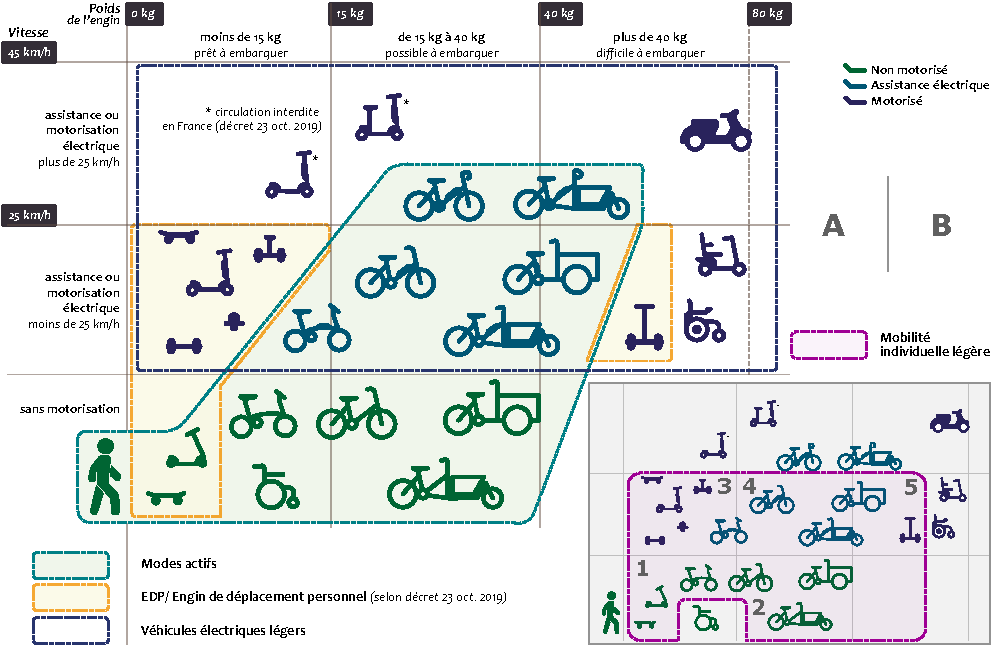
\includegraphics[width=1\columnwidth]{src/Figures/Chap-1/FR_Definition_perimetre_micromobilite.pdf}}
        \vspace{5pt}
        \begin{flushright}\scriptsize{
        Source (A)~: \textcolor{blue}{\textcite[61]{rabaud_quand_2022}}\index{Rabaud, Mathieu|pagebf}\index{Richer, Cyprien|pagebf}
        \\
        Adaptation graphique (B)~: \textcolor{blue}{Dylan Moinse (2023)}
        }\end{flushright}
    \end{figure}

    % Définition MIL
Dans ce cadre, nous proposons d’adopter une expression qui nous semble plus adaptée pour définir le périmètre de ces véhicules variés, tout en évitant les confusions liées à l’intégration de la marche ou des véhicules lourds. Cette réflexion s’appuie sur les travaux du programme ANR \acrfull{URFé}\footnote{
    Le projet, d'une durée de 42 mois, s’organise en trois volets dont le croisement permet de vérifier l’hypothèse d’un hiatus entre les pratiques effectives de mobilité et les logiques d’aménagement de l’espace~: (i) les usages, les pratiques effectives et les problèmes de sécurité, (ii) l'espace aménagé et le potentiel d'accueil vis-à-vis de la mobilité à faible impact environnemental et (iii) l'aménagement de l'espace, une action publique au prisme de la mobilité à faible impact environnemental \textcolor{blue}{\autocite{urfe_projet_2022}}.
}, sous la responsabilité scientifique de \textcolor{blue}{Frédérique Hernandez}. Ce projet de recherche examine l’hospitalité de l’espace urbain envers les nouvelles formes de mobilité à faible impact environnemental, en prenant pour terrains d’étude les aires urbaines de Lyon, de Lausanne, de Marseille~–~Aix-en-Provence et de Strasbourg \textcolor{blue}{\autocite{urfe_projet_2022}}\index{URFé@\textsl{URFé}|pagebf}. Bien que l’expression \textsl{modes de déplacement individuels à faible impact environnemental}, utilisée dans le cadre de ce projet, présente également des limites, selon nous, quant à la délimitation précise des véhicules concernés, nous avons choisi de retenir une autre notion empruntée à cette recherche~: celle de \Guillemets{mobilité individuelle légère}. Cette expression a été mise en avant lors du quatrième séminaire collectif du projet \acrshort{URFé}, tenu le 9 novembre 2022 au \acrshort{Cerema} Hauts-de-France, et nous paraît particulièrement pertinente pour regrouper les objets étudiés. En nous inspirant de la grille de lecture proposée par \textcolor{blue}{\textcite[61]{rabaud_quand_2022}}\index{Rabaud, Mathieu|pagebf}\index{Richer, Cyprien|pagebf}, dans leur chapitre intitulé \textsl{Quand les engins de déplacement personnel transforment la mobilité urbaine}, et en lien avec l’\hyperref[fig-chap1:perimetre-micromobilite]{illustration~\ref{fig-chap1:perimetre-micromobilite}} (page~\pageref{fig-chap1:perimetre-micromobilite}), nous proposons un périmètre de définition de la \Guillemets{mobilité individuelle légère} qui dépasse les cadres des \Guillemets{modes actifs}, des \acrshort{EDP}, des \Guillemets{véhicules électriques légers} et des \Guillemets{véhicules intermédiaires}. Ce périmètre vise à regrouper les véhicules relevant du vélo, de la micro-mobilité et de leurs multiples déclinaisons. Notre définition repose sur une intégration partielle des \gls{modes actifs}, à l’exclusion de la marche, ainsi que des \acrshort{EDP}, qui excluent les véhicules spécifiques aux personnes à mobilité réduite et une partie des véhicules intermédiaires dont les vitesses dépassent les limites réglementaires des engins de déplacement. Dès lors, la \Guillemets{mobilité individuelle légère} englobe une liste non exhaustive de véhicules parmi les plus populaires (voir  l’\hyperref[fig-chap1:perimetre-micromobilite]{illustration~\ref{fig-chap1:perimetre-micromobilite}}, page~\pageref{fig-chap1:perimetre-micromobilite})~:
    \begin{customitemize}
\item Véhicules à énergie musculaire de moins de 15 kilogrammes (cellule 1), comme le \textsl{skateboard}, la trottinette mécanique ou le vélo pliant~;
\item Véhicules à énergie musculaire entre 15 et 40 kilogrammes (cellule 2), comme le vélo classique, le vélo-cargo (ou biporteur) ou le triporteur~;
\item Véhicules électriques de moins de 15 kilogrammes, à une vitesse maximale de 25 kilomètres par heure (cellule 3), comme l'\textsl{hoverboard}, le monoroue, la \acrshort{TEP} ou le monocycle électrique~;
\item Véhicules à assistance électrique entre 15 et 40 kilogrammes, à une vitesse maximale de 25 kilomètres par heure (cellule 4), comme le vélo pliant électrique, le \acrshort{VAE}, le vélo-cargo électrique (ou biporteur électrique) ou le triporteur électrique~;
\item Véhicules électriques de plus de 40 kilogrammes, à une vitesse maximale de 25 kilomètres par heure (cellule 5), comme le gyropode~;
\item Services de vélos et de micro-mobilité partagés, de courte ou longue location, en libre-service avec ou sans borne d’attache (cellules 1 à 5), comme le vélo pliant en libre-service, le \acrshort{VLS}, la \acrshort{TEFF}, le \acrshort{VAE} en libre-service ou en \textsl{free-floating}, le vélo-cargo en libre-service ou le gyropode en location.
    \end{customitemize}%%Rédigé%%

    % Transition
Au sein de cette famille issue de la \Guillemets{mobilité individuelle légère}, nous conservons les sous-catégories associées au vélo et à ses diverses déclinaisons, telles que le vélo pliant, le \acrshort{VAE} ou le vélo-cargo, ainsi que la \Guillemets{micro-mobilité}, qui correspond principalement à la famille des \acrshort{EDP}. Ces véhicules partagent un certain nombre de caractéristiques communes~: ce sont des modes de déplacement individuels, bien que certains \Guillemets{modes intermédiaires} puissent accueillir un·e passager·ère supplémentaire. Leur vitesse de déplacement est limitée, ce qui permet d’instaurer une forme de proximité et d’interaction avec l’environnement urbain, s’inscrivant dans l’esprit d’une \textsl{slow city} \textcolor{blue}{\autocite[103-108]{bu_tout-voiture_2024}}\index{Bu, Ludovic|pagebf}. Par ailleurs, ces modes de déplacement se caractérisent par leur faible coût et par leur caractère plus inclusif, puisqu’ils ne nécessitent pas la possession d’un permis de conduire, ce qui les rend accessibles à un large éventail d’usager·ère·s. Ils reposent sur un système commun, conceptualisé sous le nom de \Guillemets{vélomobilité}, structuré autour d’un triptyque reposant sur les territoires, les individus et les usages \textcolor{blue}{\autocites[20-21]{rerat_au_2019}[492]{watson_how_2012}}\index{Rérat, Patrick|pagebf}\index{Watson, Matt|pagebf}. Ces véhicules présentent, par nature, un potentiel d'intermodalité~: ils sont soit facilement transportables dans les transports en commun, soit aisément adaptés au stationnement à proximité d’un nœud de transport public. C’est en raison de ces diverses qualités que nous allons désormais nous pencher plus précisément sur les synergies entre nos deux objets d’étude principaux~: les transports en commun et la mobilité individuelle légère, en nous appuyant sur le cadre théorique et stratégique du \acrshort{TOD}. Cette approche nous permettra d’examiner la manière dont le \acrshort{TOD} peut s’approprier non seulement le vélo, comme cela a été brièvement exploré dans le contexte des \textsl{Hybrid Transit Metropolises} telles que Copenhague, mais aussi les implications découlant de la récente diversification de l’offre en matière de mobilité individuelle légère. À travers cette analyse, il s’agira de mettre en lumière les liens synergiques entre ces deux systèmes.%%Rédigé%%

     % ___________________________________________
    % 1.3.
    \newpage
    \needspace{1\baselineskip} % Réserve de l'espace
    \sectionheader{Vers un \textsl{Micromobility-friendly Transit-Oriented Development}}
\section{Perspectives nouvelles pour un \textsl{Transit-Oriented Development} soutenu par l'intégration de la mobilité individuelle légère
    \label{chap1:btod}
    }

    % Introduction
L’amélioration des connaissances scientifiques relatives au développement des infrastructures de transport en commun a permis de mesurer combien elles ne suffisent pas, à elles seules, à constituer une alternative viable à l’\Guillemets{autosolisme}\footnote{
    L'\Guillemets{autosolisme} est le fait de circuler en automobile, non accompagné·e. C'est un usage dérivé du mot \Guillemets{autosoliste}. Un dictionnaire militant définit ce terme comme \Guillemets{\textsl{l'action de se déplacer seul au volant d’une voiture, et d’encombrer, ainsi, l’espace collectif, de polluer, de faire du bruit, de stresser pour le profit d’une personne unique~: le chauffeur !}} \textcolor{blue}{\autocite{carfreefr_dictionnaire_2008}}\index{Carfree.fr@\textsl{Carfree.fr}|pagebf}. Occasionnellement, l'antonyme \Guillemets{automultisme} peut apparaître, mais il est plus courant de parler de \Guillemets{covoiturage}.
}, en tout point du territoire \textcolor{blue}{\autocite[8]{molino_pratiques_2015}}\index{Molino, Marie|pagebf}\index{Rampon, Anne-Sophie|pagebf}\index{Cipolla, Romain|pagebf}. Le développement traditionnel de l’offre de transport public appelle une action simultanée sur la demande. En effet, pour réduire efficacement le trafic automobile, plusieurs stratégies peuvent être envisagées. Soit une réduction de l'aire urbanisée, difficilement faisable et acceptable. Soit une densification de la desserte en transport public, qui risque cependant de nuire à la performance du réseau en raison d'un nombre important d'arrêts, et ainsi compromettre sa compétitivité face à l'automobile. Soit une amélioration de l’accessibilité aux stations, option jugée la plus réaliste \textcolor{blue}{\autocite[10]{verbavatz_critical_2019}}\index{Verbavatz, Vincent|pagebf}\index{Barthelemy, Marc|pagebf}. Il ressort des recherches que le facteur déterminant du transfert modal de la voiture vers les transports en commun est l’accessibilité aux stations, plutôt que l’amélioration qualitative du service \textcolor{blue}{\autocite[146]{brons_access_2009}}\index{Brons, Martijn|pagebf}\index{Givoni, Moshe|pagebf}\index{Rietveld, Piet|pagebf}. Cette observation rejoint le principe fondateur, selon lequel la mobilité au sein des quartiers de gare, et en particulier la priorité donnée à la marche et au vélo combinés, constitue un levier central pour la réussite d’une intervention de type \acrshort{TOD}. Pourtant, ces modes de déplacement, bien qu’essentiels à la planification urbaine orientée vers le transport public, restent souvent invisibilisés ou traités de manière banale, alors qu’ils jouent un rôle déterminant dans le succès ou l’échec d’un projet \acrshort{TOD} \textcolor{blue}{\autocite[34]{schlossberg_comparing_2004}}\index{Schlossberg, Marc|pagebf}\index{Brown, Nathaniel|pagebf}. Face à l’\Guillemets{explosion périurbaine}, la performance et l’attractivité des réseaux de transport public se sont considérablement amoindries, en raison de l’allongement des distances et de la dispersion des pôles d’emplois \textcolor{blue}{\autocite[13]{bentayou_transit-oriented_2015}}\index{Bentayou, Gilles|pagebf}. Dans ce contexte, l’approche intermodale intégrant le vélo apparaît comme la réponse la plus adaptée aux enjeux des \Guillemets{premiers et derniers kilomètres}. Le vélo et le transport public doivent ainsi entretenir une relation symbiotique~: au-delà d’un simple mode de rabattement, le vélo doit être pleinement intégré à l’expérience de voyage, en raison de la forte compétitivité de cette combinaison modale face à la voiture individuelle \textcolor{blue}{\autocite[208]{kager_characterisation_2016}}\index{Kager, Roland|pagebf}\index{Bertolini, Luca|pagebf}\index{te Brömmelstroet, Marco|pagebf}. Au-delà du seul vélo, il est aujourd’hui opportun d’évaluer si les \Guillemets{nouvelles mobilités} qui gravitent autour de celui-ci peuvent renforcer cette dynamique. Ces modes émergents pourraient en effet s’inscrire dans une logique de \Guillemets{bouquet d’offres de modes et de services} visant à maximiser les bénéfices d’un système de mobilité alternatif plus sobre dans la consommation des ressources \textcolor{blue}{\autocite[134]{litman_new_2021}}\index{Litman, Todd|pagebf}.%%Rédigé%%

    % Annonce du plan
Dans un premier temps, nous allons parcourir la règle arbitraire des périmètres accessibles à pied autour des aires \acrshort{TOD}\textcolor{blue}{s} et, plus largement, la nécessité d’étendre les quartiers de gare grâce à une approche intermodale. Nous allons voir que les études montrent combien la marche combinée peut s’étendre bien au-delà du périmètre géographique qui lui est généralement attribué, tout en soulignant que sa portée, bien que pertinente, demeure insuffisante pour garantir un accès optimal aux nœuds de transport, dans un contexte de périurbanisation. Il apparaît ainsi essentiel d’intégrer d’autres modes de déplacement permettant d’atteindre des destinations plus éloignées, afin de renforcer la complémentarité modale et d’optimiser l’accessibilité aux nœuds (\hyperref[chap1:btod-limites-tod]{section sur une relecture de la marche combinée, page~\pageref{chap1:btod-limites-tod}}). Dans cette perspective, nous allons examiner les avantages comparatifs de la mobilité individuelle légère, qui apparaît comme une alternative particulièrement appropriée pour limiter le recours excessif à l’automobile. Cette réflexion va nous conduire à aborder la récente déclinaison d'un \acrfull{B-TOD}, ou d'un urbanisme orienté vers les réseaux de transport en commun et intégrant le vélo, qui met en avant les potentialités du vélo dans l’extension des aires d’influence des stations de transport public. Enfin, au regard de la diversité modale évoquée précédemment dans ce chapitre, nous allons nous interroger sur l'intérêt d'une conceptualisation plus englobante intégrant la mobilité individuelle légère, au travers d’un \acrfull{M-TOD} (\hyperref[chap1:btod-definition]{section sur une combinaison modale tirant parti de la vitesse et d'une accessibilité \Guillemets{porte-à-porte}, page~\pageref{chap1:btod-definition}}).%%Rédigé%%

    % 1.3.1.
    \needspace{1\baselineskip} % Réserve de l'espace
\subsection{Vers un \Guillemets{éclatement de la bulle} des poches piétonnières
    \label{chap1:btod-limites-tod}
    }

    % Introduction
La notion de \Guillemets{poche piétonnière} (\textsl{pedestrian pocket}), antérieure au \acrshort{TOD}, repose sur la délimitation d’une zone au sein de laquelle la marche constitue le mode de déplacement privilégié et où se concentrent les principales activités quotidiennes \textcolor{blue}{\autocite[3]{kelbaugh_pedestrian_1989}}\index{Kelbaugh, Doug|pagebf}. Bien que largement intégrée au concept d’aménagement, l’aire d’influence piétonne des gares est souvent définie sur la base de frontières arbitraires, qui ne reflètent pas nécessairement les pratiques réelles des voyageur·se·s et peuvent ainsi entraîner une inadéquation entre le périmètre des quartiers de gare et les parcours effectifs des usager·ère·s. À partir de ce constat, nous rejoignons la littérature scientifique récente qui appelle à reconsidérer la portée réelle de la marche combinée. En effet, les cheminements piétons vers et depuis une station ne se limitent pas à l’échelle immédiate de la gare, mais influencent également la distance spatio-temporelle que les usager·ère·s sont disposé·e·s à parcourir \textcolor{blue}{\autocite[52]{el_hadeuf_ville_2017}}\index{El Hadeuf, Mounya|pagebf}\index{Laterrasse, Jean|pagebf}. Dans cette perspective, nous proposons d’exploiter cet \Guillemets{éclatement de la bulle} \textcolor{blue}{\autocite[33]{guerra_half-mile_2012}}\index{Guerra, Erick|pagebf} comme une une occasion de redéfinir l’aménagement des territoires en adoptant une approche systémique, ou intégratrice \textcolor{blue}{\autocite[56]{kaufmann_retour_2014}}\index{Kaufmann, Vincent|pagebf} sur les atouts que présente l'intermodalité-voyageur·se·s. Une telle démarche permettrait d’envisager des espaces véritablement orientés vers les transports en commun, définis à une échelle spatiale plus pertinente et susceptibles d’optimiser le report modal vers le réseau de transport public.%%Rédigé%%

    % 1.3.1.1.
    \needspace{1\baselineskip} % Réserve de l'espace
\subsubsection*{Remise en question de la \textsl{doxa} de \Guillemets{poches piétonnières} confinées
    \label{chap1:btod-limites-tod-marche-restreinte}
    }

    % Doxa
En France, comme nous l’avons observé, nous assistons souvent à une mise en œuvre de principes proches du \Guillemets{\acrshort{TOD} sans le dire} \textcolor{blue}{\autocite[273]{lo_feudo_scenario_2014}}\index{Lo Feudo, Fausto|pagebf}\index{Menerault, Philippe|pagebf}\index{L'Hostis, Alain|pagebf}\index{Festa, Demetrio Carmine|pagebf}. Cette multiplicité d’interventions sur le territoire, apparentée à ce concept d’aménagement, se limite fréquemment à des actions ponctuelles telles que le renouvellement architectural des gares ou le réaménagement des espaces adjacents, accordant moins d’attention aux échelles plus larges, notamment le quartier de gare et son insertion dans la métropole \textcolor{blue}{\autocite[50]{bentayou_transit-oriented_2015}}\index{Bentayou, Gilles|pagebf}. Lorsque les projets \acrshort{TOD}\textcolor{blue}{s} ciblent spécifiquement les aires d’influence piétonnes des nœuds de transport en commun, ils s’appuient sur une référence communément admise~: celle des 500 mètres ou des 800 mètres, la dernière équivalant à 10 minutes de marche \textcolor{blue}{\autocite[1]{lhostis_perimetres_2016}}\index{L'Hostis, Alain|pagebf}, souvent définie comme une \Guillemets{aire pédestre} (\textsl{pedestrian pocket}). \textcolor{blue}{Peter} \textcolor{blue}{\textcite[56]{calthorpe_next_1993}}\index{Calthorpe, Peter|pagebf} préconise des communautés conçues à moins de 600 mètres (environ 2~000 pieds) d’un arrêt. \textcolor{blue}{\textcite[12]{bertolini_cities_2015}}\index{Bertolini, Luca|pagebf}\index{Spit, Tejo|pagebf}, dans leur ouvrage \foreignlanguage{english}{\textsl{Cities on Rails: The Redevelopment of Railway Stations and their Surroundings}} confirment qu’un périmètre de dix minutes à pied constitue une distance-temps acceptable pour accéder à une station. Une revue de littérature sur les périmètres d’action autour des gares, réalisée par \textcolor{blue}{\textcite[102]{guerra_half-mile_2012}}\index{Guerra, Erick|pagebf}\index{Cervero, Robert|pagebf}\index{Tischler, Daniel|pagebf}, montre cependant que cette norme des 400 à 800 mètres est fréquemment mobilisée sans qu’elle repose nécessairement sur des justifications techniques. Pourtant, comme nous l’avons vu dans l’évolution de la pensée du \acrshort{TOD}, l’un des \Guillemets{5Ds} associés à ce concept, la distance aux stations (\textsl{Distance to Transit}), est une équation centrale pour mesurer l’accessibilité au transport en commun \textcolor{blue}{\autocite[267]{ewing_travel_2010}}\index{Ewing, Reid|pagebf}\index{Cervero, Robert|pagebf}. Au cours de la dernière décennie, des recherches ont cherché à remettre en question cette norme internationale du \Guillemets{800 mètres} (\textsl{half-mile distance}), devenue un standard dans les projets \acrshort{TOD}\textcolor{blue}{s} \textcolor{blue}{\autocite[102]{guerra_half-mile_2012}}\index{Guerra, Erick|pagebf}\index{Cervero, Robert|pagebf}\index{Tischler, Daniel|pagebf}. L’objectif est d’\Guillemets{éclater la bulle} piétonnière (\textsl{busting the bubble}) \textcolor{blue}{\autocite[33]{guerra_half-mile_2012}}\index{Guerra, Erick|pagebf}, c’est-à-dire de dépasser les limites envisagées de la marche combinée. Cela ouvre la voie à un modèle \acrshort{TOD} réinterprété, dépassant la métaphore spatiale de la \Guillemets{bulle cible} (\textsl{the bull’s eye concept}) \textcolor{blue}{\autocite[28]{curtis_transit_2009}}\index{Curtis, Carey|pagebf}\index{Renne, John Luciano|pagebf}\index{Bertolini, Luca|pagebf}.%%Rédigé%%

    % Documents d'urbanisme
Cette règle communément admise, reposant sur le périmètre piétonnier de 800 mètres, est fréquemment appliquée et visible dans les documents d’orientation en matière d’aménagement du territoire. Les aménageur·se·s utilisent typiquement cette limite comme périmètre d’action urbaine autour des gares \textcolor{blue}{\autocite[40]{olszewski_using_2005}}\index{Olszewski, Piotr~S.|pagebf}\index{Wibowo, Sony Sulaksono|pagebf}. Déjà dans le \textsl{Schéma Régional des Transports} de l’ancienne \textcolor{blue}{\textcite[21]{region_nord-pas-de-calais_schema_2006}}\index{Région Nord-Pas-de-Calais@\textsl{Région Nord-Pas-de-Calais}|pagebf}, la marche était identifiée comme un mode à privilégier pour les trajets en rabattement, dits de \Guillemets{courte distance}, vers les arrêts de bus ou de car, les gares et les pôles d’échange. Le \acrfull{PDU} 2010-2020 de la \acrfull{MEL} a intégré cette approche en définissant des \acrfull{DIVAT}, correspondant à des espaces stratégiques situés autour des gares métropolitaines, des stations de métro et de tramway, ainsi que des arrêts de \acrfull{BHNS}. Ces périmètres stratégiques prennent alors la forme d’un cercle de 500 mètres de rayon \textcolor{blue}{\autocite[39]{lmcu_plan_2011}}\index{LMCU@\textsl{LMCU}|pagebf}. En cohérence avec ce \acrshort{PDU}, les \acrshort{DIVAT} ont été fidèlement repris dans le \acrfull{PLH} 2012-2018 de la \acrshort{MEL}, avec un élargissement aux arrêts de bus enregistrant plus de soixante passages quotidiens, tous sens confondus \textcolor{blue}{\autocite[4]{lmcu_2e_2012}}\index{LMCU@\textsl{LMCU}|pagebf}. Ces principes ont ensuite été intégrés dans le \acrfull{PLUi} de 2020 de l’\acrfull{EPCI}, renforçant ainsi la cohérence entre les différents outils de planification territoriale \textcolor{blue}{\autocite[44]{metropole_europeenne_de_lille_plan_2019-3}}\index{LMCU@\textsl{LMCU}|pagebf}. Cependant, certaines études stratégiques ont revu ces périmètres de gare pour les adapter à des contextes variés. Par exemple, l’Observatoire des quartiers de gare du Grand Paris Express avait d'abord défini un périmètre de 800 mètres à vol d’oiseau pour les 69 gares en construction \textcolor{blue}{\autocite[1]{apur_observatoire_2017}}\index{Apur@\textsl{Apur}|pagebf}. Ce cadre a ensuite évolué pour proposer deux autres niveaux~: 500 mètres pour stations situées dans l'hypercentre et 1~000 mètres pour les gares \acrfull{RER} et celles du Grand Paris Express \textcolor{blue}{\autocite[13]{apur_observatoire_2018}}\index{Apur@\textsl{Apur}|pagebf}. Enfin, une attention particulière a été accordée à un rayon de 2~000 mètres pour l’échelle cyclable \textcolor{blue}{\autocite[22]{apur_observatoire_2018}}\index{Apur@\textsl{Apur}|pagebf}.%%Rédigé%%

    % Eclatement aires primaires
D'aucun·e·s considèrent que la marche combinée peut atteindre des distances spatio-temporelles bien supérieures à celles dictées par la règle d’origine anglo-saxonne des 400 ou 800 mètres, ou encore des 10 minutes, au sein du périmètre de l’\Guillemets{aire primaire} telle qu’imaginée par \textcolor{blue}{Peter} \textcolor{blue}{\textcite[56]{calthorpe_next_1993}}\index{Calthorpe, Peter|pagebf}. Dans une revue de littérature, le chercheur en géographie, spécialisé dans l'aménagement et la mobilité, \textcolor{blue}{Alain} \textcolor{blue}{\textcite[5]{lhostis_perimetres_2016}}\index{L'Hostis, Alain|pagebf} met en évidence que certaines gares ferroviaires ou stations de métro européennes enregistrent des déplacements à pied atteignant aisément un à deux kilomètres de distance spatiale. La pratique de la marche combinée (\textsl{walk-and-ride}) autour des nœuds de transport en commun bien desservis, bénéficiant de fréquences élevées, d’une desserte étendue et d’une bonne accessibilité, est ainsi marquée par un étirement de ses distances socialement acceptées. Ces quartiers, à la fois denses, mixtes et avec une haute qualité de conception de ses espaces publics, notamment en termes de \gls{marchabilité}, incarnent les principes des quartiers \acrshort{TOD}\textcolor{blue}{s}. Les recherches montrent que dans ce contexte, les trajets à pied dépassent largement le seuil des 800 mètres traditionnellement admis \textcolor{blue}{\autocites[79]{ker_myths_2003}[7]{lhostis_perimetres_2016}[30]{hasiak_access_2019}}\index{Hasiak, Sophie|pagebf}\index{L'Hostis, Alain|pagebf}\index{Ker, Ian|pagebf}\index{Ginn, Simon|pagebf}.%%Rédigé%%

    % Figure Corridor Piéton
    \begin{carte}[h!]\vspace*{4pt}
        \caption{Extension du quartier de gare par la valorisation d'un corridor densifié et accessible à pied.}
        \label{fig-chap1:tod-corridor-pieton}
        \centerline{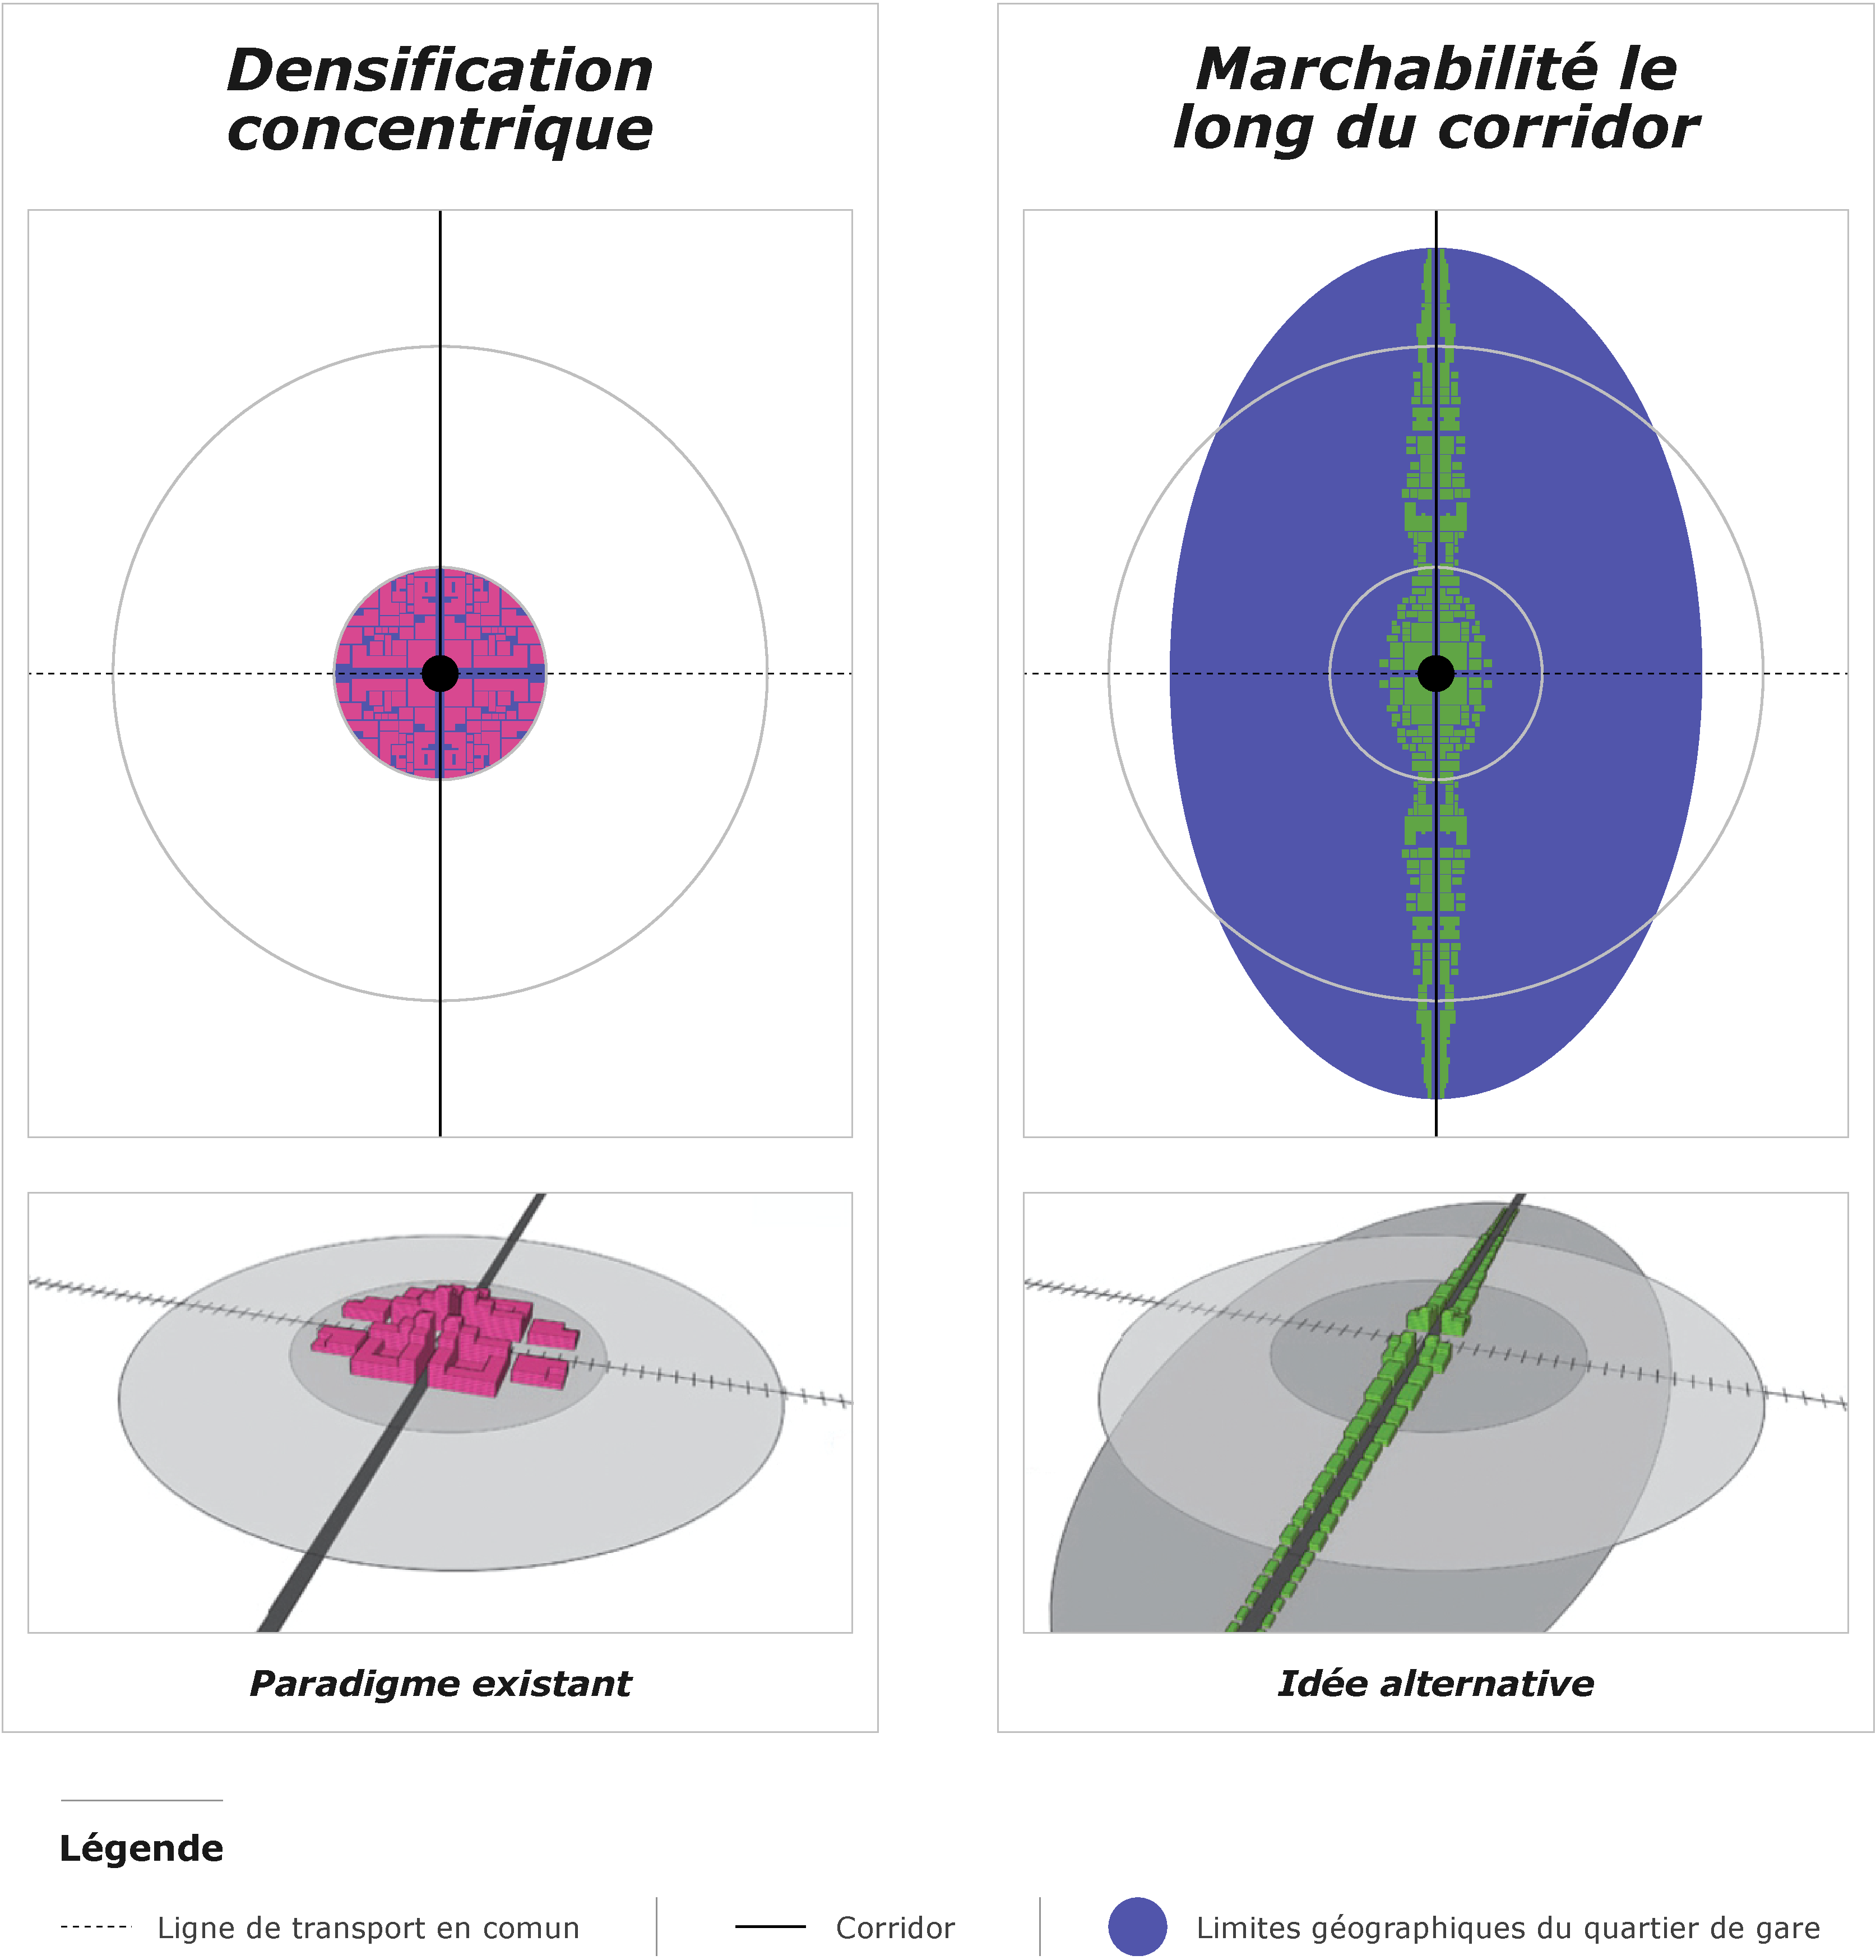
\includegraphics[width=1\columnwidth]{src/Figures/Chap-1/FR_Corridor_pieton.pdf}}
        \vspace{5pt}
        \begin{flushright}\scriptsize{
        Source~: \textcolor{blue}{\textcite[163]{park_can_2015}}\index{Park, Sungjin|pagebf}\index{Deakin, Elizabeth|pagebf}\index{Jang, Kitae|pagebf}
        \\
        Adaptation graphique~: \textcolor{blue}{Dylan Moinse (2025)}
        }\end{flushright}
    \end{carte}

    % Exemples
De nombreuses études s’intéressent aujourd’hui à la distance parcourue par les voyageur·se·s pour se rendre ou sortir à pied d'une station de transport en commun, soutenant généralement une sous-calibration globale des périmètres piétonniers traditionnellement admis autour de ces nœuds. En moyenne, les piéton·ne·s qui accèdent à une gare ou une station de métro parcourent 1 kilomètre, que ce soit à San Francisco \textcolor{blue}{\autocite[5]{cervero_walk-and-ride_2001}}\index{Cervero, Robert|pagebf} ou à Singapour \textcolor{blue}{\autocite[41]{olszewski_using_2005}}\index{Olszewski, Piotr~S.|pagebf}\index{Wibowo, Sony Sulaksono|pagebf}. En s’appuyant sur le 85\textsuperscript{e} centile de la distribution cumulative des distances parcourues, des études ont montré qu’une distance de 1 kilomètre (soit environ 12 minutes à pied) est jugée acceptable autour des stations de métro à Beijing \textcolor{blue}{\autocite[720]{yang_study_2013}}\index{Yang, Rongrong|pagebf}\index{Yan, Hai|pagebf}\index{Xiong, Wen|pagebf}\index{Liu, Tao|pagebf}, tandis que des distances légèrement supérieures, de 1,2 (en rabattement) et 1,1 kilomètres (en diffusion), sont observées autour des gares à Montréal \textcolor{blue}{\autocite[9]{el-geneidy_pedestrian_2009}}\index{El-Geneidy, Ahmed~M.|pagebf}\index{Tétreault, Paul|pagebf}\index{Surprenant-Legault, Julien|pagebf}. Au sud-est de l’Angleterre, les distances atteignent même 1,6 kilomètre autour des gares \textcolor{blue}{\autocite[14]{bunn_how_2015}}\index{Bunn, Nick|pagebf}\index{Wakenshaw, Gareth|pagebf}. Dans le cas du Nord-Pas-de-Calais, le 90\textsuperscript{e} centile des voyageur·se·s ferroviaires révèle que les distances parcourues peuvent atteindre 20 minutes à pied, contre une moyenne observée de 11 minutes \textcolor{blue}{\autocite[17]{hasiak_estimation_2018}}\index{Hasiak, Fabrice|pagebf}\index{Lannoy, Arnaud|pagebf}\index{Bodard, Géraldine|pagebf}\index{Palmier, Patrick|pagebf}. Ces variations témoignent de l’influence majeure de certains paramètres de l’environnement urbain, qui peuvent dilater ou contracter ces distances perçues \textcolor{blue}{\autocite[17]{soest_exploring_2020}}\index{Soest, Dennis van|pagebf}\index{Tight, Miles~R.|pagebf}\index{Rogers, Christopher~D.~F.|pagebf}. Déjà en 1984, \textcolor{blue}{Richard~k.} \textcolor{blue}{\textcite[23-59]{untermann_accommodating_1984}}\index{Untermann, Richard~K.|pagebf}, dans son livre \foreignlanguage{english}{\textsl{Accommodating the Pedestrian: Adapting Towns and Neighborhoods for Walking and Biking}}, montrait que la portée maximale de la marche dans les territoires périurbains, souvent confinée dans des seuils rigides de 400, 500 ou 800 mètres, pouvait être considérablement étendue~–~voire doublée~–~en aménageant des espaces urbains attrayants et des corridors agréables pour les piéton·ne·s. Les recherches plus récentes confirment que la diversité urbaine joue un rôle clé. Par exemple, une étude comparative menée entre Beijing, Tianjin et Shenzhen indique que les voyageur·se·s à pied doublent souvent leurs distances parcourues lorsque l’environnement urbain présente une mixité élevée, avec des commerces et des bureaux à proximité des stations \textcolor{blue}{\autocite[12]{zacharias_local_2017}}\index{Zacharias, John|pagebf}\index{Zhao, Qi|pagebf}. De même, en Australie comme aux États-Unis, les voyageur·se·s sont disposé·e·s à parcourir jusqu’à 800 mètres supplémentaires lorsque l’environnement urbain suit les principes du \acrshort{TOD} \textcolor{blue}{\autocite[33]{canepa_bursting_2007}}\index{Canepa, Brian|pagebf}. L’amélioration des éléments de \Guillemets{micro-marchabilité} (\textsl{microwalkability}), notamment par l’aménagement stratégique de corridors piétonniers, apparaît comme un levier déterminant pour étendre ces périmètres spatiaux. Ainsi, \textcolor{blue}{\textcite[163]{park_can_2015}}\index{Park, Sungjin|pagebf}\index{Deakin, Elizabeth|pagebf}\index{Jang, Kitae|pagebf} montrent qu’il est possible d’encourager les usager·ère·s du transport public à parcourir des distances bien plus importantes en améliorant ces infrastructures piétonnes (voir la \hyperref[fig-chap1:tod-corridor-pieton]{carte~\ref{fig-chap1:tod-corridor-pieton}}, page~\pageref{fig-chap1:tod-corridor-pieton}). Par exemple, l’aménagement de rues piétonnes autour des gares permet d’augmenter de 20~\% la portée jugée acceptable de la marche à destination des gares aux États-Unis, et jusqu’à 120~\% en Allemagne \textcolor{blue}{\autocite[151]{zielstra_comparative_2011}}\index{Zielstra, Dennis|pagebf}\index{Hochmair, Hartwig~H.|pagebf}.%%Rédigé%%

    % Conclusion + Transition
Qu’il s’agisse d’une aire d’influence accessible à pied, représentée sous la forme d’une étendue euclidienne (cercle) ou calculée sur la base de la voirie (isodistance ou isochrone), la règle arbitraire des 800 mètres ou des 10 minutes à pied relève davantage d’un artéfact historique que d’une construction analytique et statistique \textcolor{blue}{\autocite[102]{guerra_half-mile_2012}}\index{Guerra, Erick|pagebf}\index{Cervero, Robert|pagebf}\index{Tischler, Daniel|pagebf}. Cette règle, bien que communément utilisée, démontre ses limites. En effet, si le périmètre d'\Guillemets{aire primaire} des stations de transport en commun évalué à 800 mètres n'est pas fondamentalement erroné~–~les moyennes enregistrées pour le rail interurbain atteignant souvent 1~000 mètres~–, la véritable différence réside dans la méthode de mesure. En adoptant une approche basée sur la distance \Guillemets{acceptable} (en considérant les 85 ou 90\textsuperscript{e} centiles) plutôt que simplement observable, il apparaît clairement que les périmètres piétonniers traditionnels sous-évaluent les véritables distances parcourues et vécues par les usager·ère·s. Par exemple, une étude démontre que les seuils traditionnels de 400 et 800 mètres sous-estiment de 30~\% la couverture réelle du transport public accessible à pied dans la région montréalaise \textcolor{blue}{\autocite[20]{el-geneidy_new_2014}}\index{El-Geneidy, Ahmed~M.|pagebf}\index{Grimsrud, Michael|pagebf}\index{Wasfi, Rania|pagebf}\index{Tétreault, Paul|pagebf}\index{Surprenant-Legault, Julien|pagebf}. Cela met en évidence la nécessité de dépasser la conception classique de la marche. En France, bien que la durée moyenne des déplacements piétons soit de 13 minutes, il convient de différencier la marche monomodale et la marche combinée, utilisée comme mode de liaison vers les stations de transport en commun. En effet, si quatre déplacements piétons sur cinq en France durent moins de 15 minutes, ceux associés à la marche combinée atteignent fréquemment 20 minutes autour des gares \textcolor{blue}{\autocite[23]{solere_mobilite_2010}}\index{Solere, Régis de|pagebf}\index{Papon, Francis|pagebf}. Cette portée accrue de la marche combinée est de plus en plus reconnue dans la recherche académique, qui la considère extensible en fonction de facteurs favorisant le potentiel \acrshort{TOD} des territoires, tels que la densité urbaine, la mixité fonctionnelle ou la qualité des infrastructures piétonnes. Toutefois, dans les quartiers périphériques, où les distances requises pour accéder au transport public sont bien plus importantes, la marche seule ne suffit pas à corriger ces déséquilibres \textcolor{blue}{\autocite[85]{cervero_bike-and-ride_2013}}\index{Cervero, Robert|pagebf}\index{Caldwell, Benjamin|pagebf}\index{Cuellar, Jesus|pagebf}. Pour dépasser la dichotomie entre la marche et le transport public en zone centrale, et la voiture en intermodalité en zone périurbaine, le vélo peut constituer le maillon manquant de la chaîne intermodale. Or, bien que la littérature académique et technique se concentre presque exclusivement sur l’accessibilité des stations à pied, l’accessibilité à vélo demeure largement marginalisée et sous-étudiée \textcolor{blue}{\autocite[283]{martens_bicycle_2004}}\index{Martens, Karel|pagebf}. Cette lacune représente un défi à relever pour intégrer pleinement le vélo dans les stratégies d’accessibilité et d’intermodalité, en particulier dans les territoires où les distances dépassent les capacités traditionnelles de la marche.%%Rédigé%%

    % 1.3.1.2.
    \needspace{1\baselineskip} % Réserve de l'espace
\subsubsection*{Corriger les faiblesses du transport public par une approche intermodale
    \label{chap1:btod-definition-intermodalite}
    }

    % Limitations de la marche
Au regard des limitations liées à la portée de la marche, qui rend parfois l’accès aux stations de transport en commun contraignant, l’efficacité du \acrshort{TOD} est aujourd’hui interrogée. En effet, la croissance urbaine des territoires s’est majoritairement appuyée sur des distances adaptées à l’échelle de l’automobile, se traduisant par un étalement urbain souvent assimilé à une forme de \Guillemets{suburbanisation}. Par ailleurs, le transport public, bien qu’efficace sur certains aspects, ne dispose pas de l’ensemble des avantages de flexibilité associés à l’automobile \textcolor{blue}{\autocite[209]{heran_retour_2015}}\index{Héran, Frédéric|pagebf}. Cette situation remet en question la capacité du modèle urbain à lutter efficacement contre la dépendance aux modes motorisés. Les transports en commun ne représentent qu’une solution partiellement adaptée pour réduire le recours excessif à l’automobile. Une alternative réside alors dans la promotion de l’intermodalité, qui permettrait de pallier la rigidité du réseau de transport en commun \textcolor{blue}{\autocite[17]{wiel_comment_1998}}\index{Wiel, Marc|pagebf} et d’améliorer l’efficacité globale du système de mobilité \textcolor{blue}{\autocite[82]{oostendorp_combining_2018}}\index{Oostendorp, Rebekka|pagebf}\index{Gebhardt, Laura|pagebf}. En effet, l’intermodalité contribue à étendre l’aire d’influence des nœuds en y intégrant des solutions complémentaires \textcolor{blue}{\autocite[16]{amar_homo_2016}}\index{Amar, Georges|pagebf}, ce qui pourrait renforcer leur pertinence dans des contextes urbains et périurbains marqués par la dépendance automobile.%%Rédigé%%

    % Intermodalité
L’interconnexion désigne la liaison entre deux ou plusieurs réseaux de transport hétérogènes dans leurs dimensions techniques, organisationnelles et institutionnelles, souvent associés à des échelles de mobilité distinctes \textcolor{blue}{\autocites[]{dupuy_reseaux_1988}{varlet_interconnexion_1992}}\index{Dupuy, Gabriel|pagebf}\index{Varlet, Jean|pagebf}. L’intérêt de cette transition entre différents régimes de mobilité réside dans la capacité à dépasser la simple juxtaposition de réseaux monomodaux qui n'ont pas été pensés pour être coordonnés. Cette approche permet de mieux comprendre le \Guillemets{concept-interface} qui met en relation plusieurs vitesses de déplacement et plusieurs échelles spatiales \textcolor{blue}{\autocite[156]{peters_time_1960}}\index{Peters, Peter Frank|pagebf}. Cette intégration intermodale donne lieu à la formation d’un méta-réseau, défini comme un réseau de réseaux effectifs. Il s’agit d’un emboîtement multiscalaire de systèmes qui, par leur interconnexion, créent un mégasystème intégré \textcolor{blue}{\autocite[89]{ageron_intermodalite-voyageurs_2013}}\index{Ageron, Pierre|pagebf}\index{Varlet, Jean|pagebf}. L’intermodalité-voyageur·se·s devient ainsi un objet-système, comme organisation actorielle géographiquement située, génératrice de lieux et de pratiques \textcolor{blue}{\autocite[15]{varlet_interconnexion_1992}}\index{Varlet, Jean|pagebf}. Liée en grande partie à un mode de transport en commun, l’intermodalité-voyageur·se·s est reconnue comme l’option la plus économique en termes de ressources, en tenant compte du temps de parcours, du coût ou de la consommation d’énergie pour effectuer un déplacement entre un point A et un point B \textcolor{blue}{\autocite[73]{oostendorp_combining_2018}}\index{Oostendorp, Rebekka|pagebf}\index{Gebhardt, Laura|pagebf}. En ce sens, la mise en correspondance, l’interconnexion et l’intermodalité des réseaux constituent des facteurs d’efficacité qui s’inscrivent dans le cadre du principe de \Guillemets{reliance}. Ce dernier, en tant que créateur de liens et de synergies entre des flux de nature variée, sous-tend de nouvelles formes d’optimisation des réseaux \textcolor{blue}{\autocite[16-17]{amar_homo_2016}}\index{Amar, Georges|pagebf}. Cette évolution s’accompagne d’une diversification modale croissante, favorisée par des processus de (ré)invention, d’innovation technique et servicielle, ainsi que par des phénomènes d’hybridation modale. Ces dynamiques dépassent la vision binaire du simple report modal de la voiture au transport en commun, pour promouvoir une approche multimodale et intermodale \textcolor{blue}{\autocite{richer_dossier_2021}}\index{Richer, Cyprien|pagebf}.

    % Figure fonctions et composantes intermodalité
    \begin{figure}[h!]\vspace*{4pt}
        \caption{Fonctions et composantes du système intermodal.}
        \label{fig-chap1:composantes-fonctions-intermodalite}
        \centerline{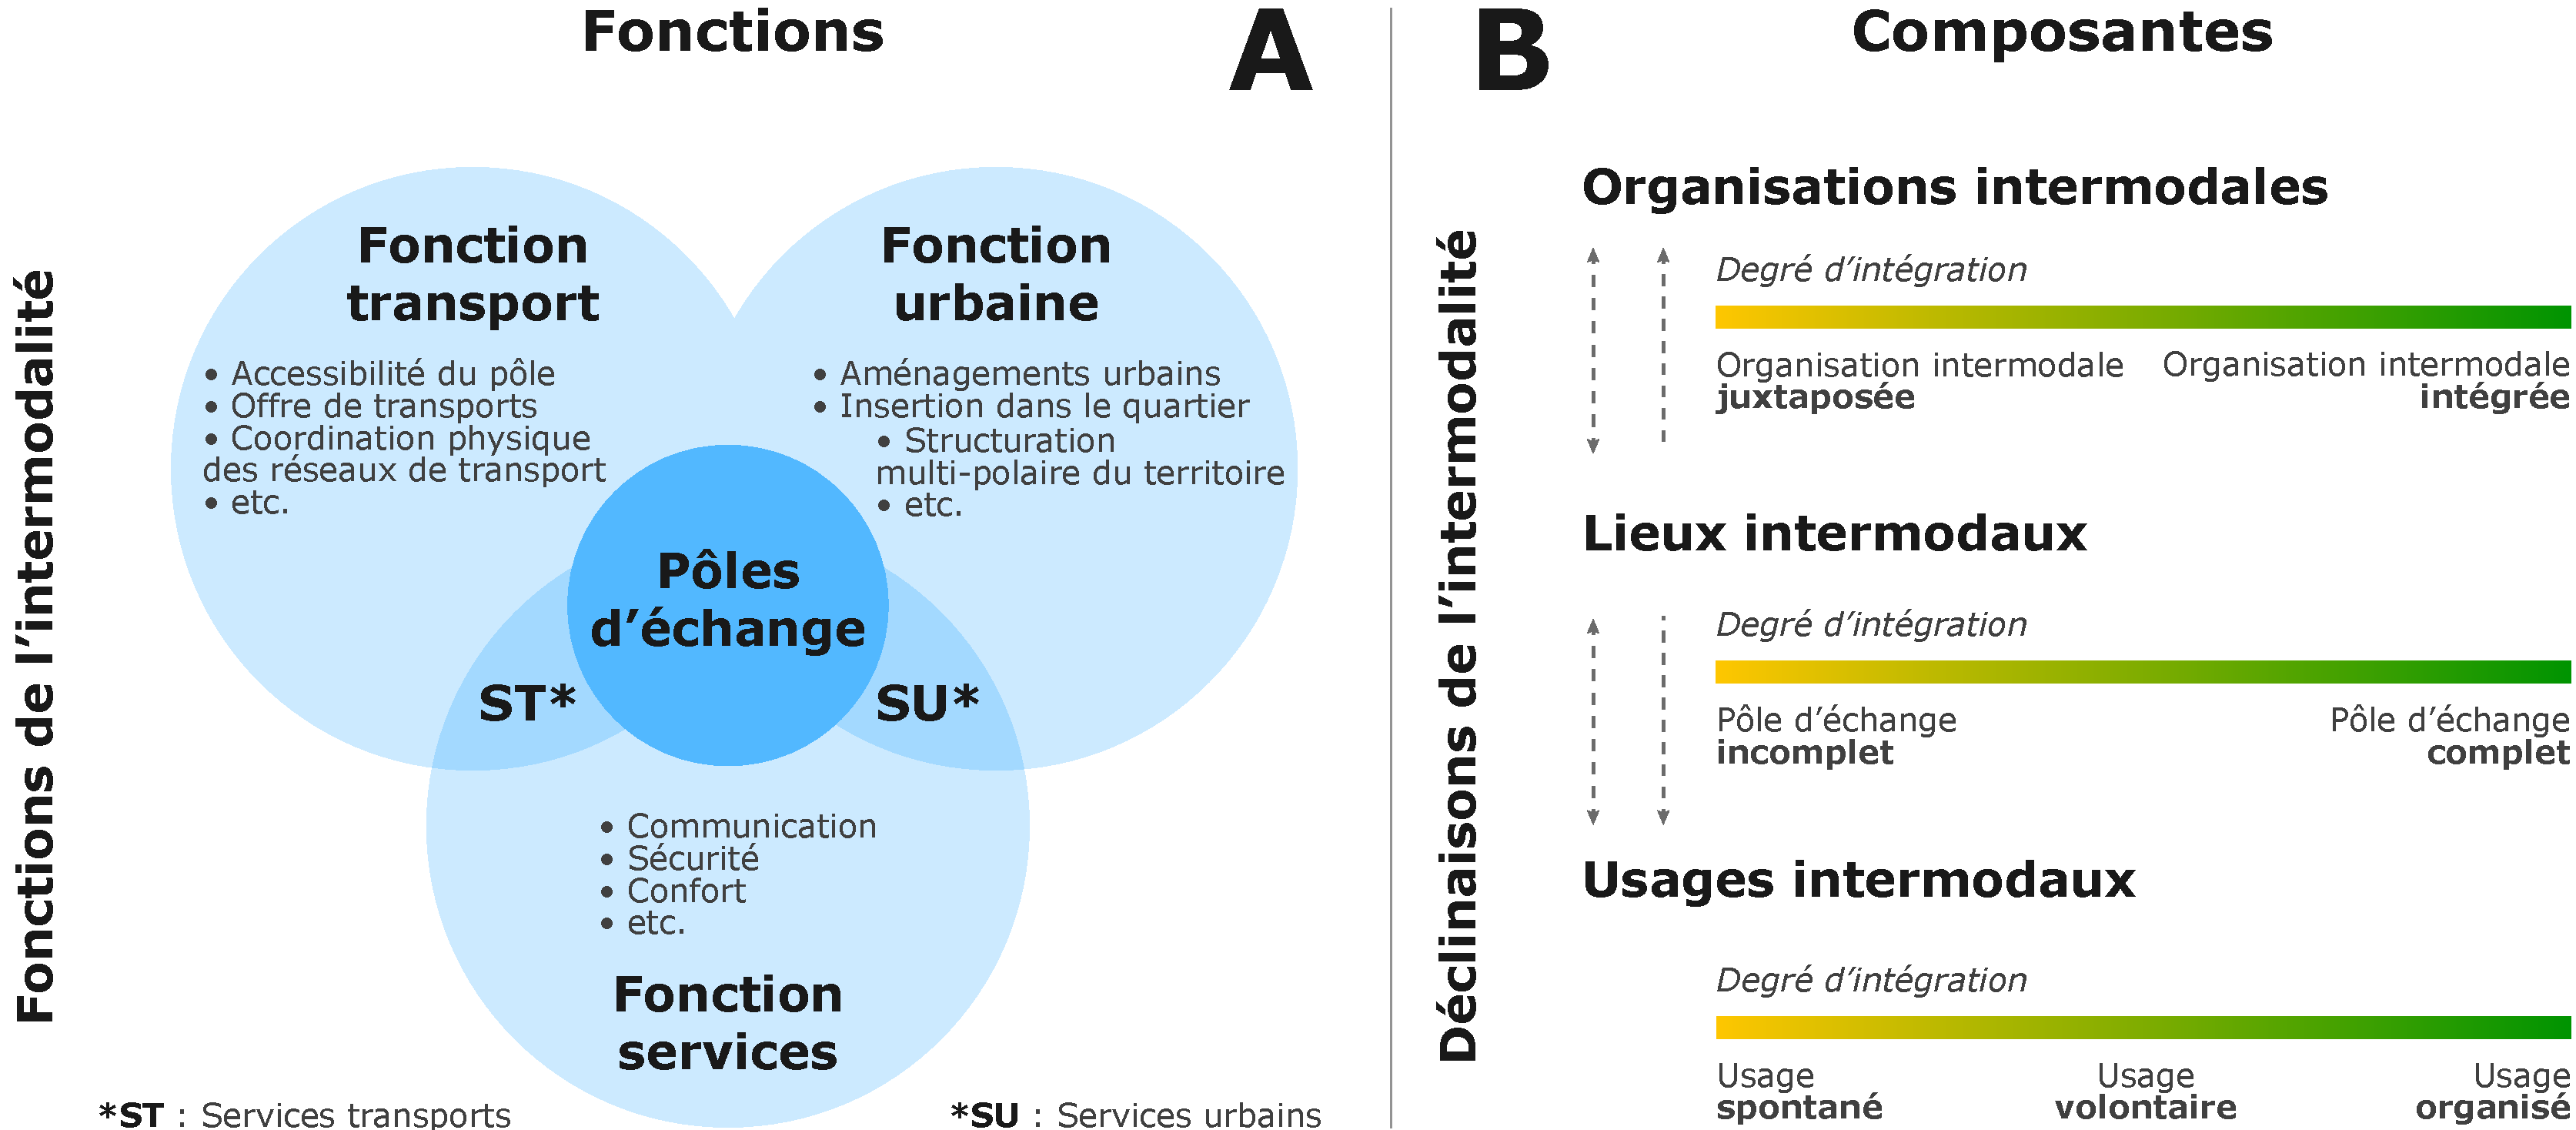
\includegraphics[width=1\columnwidth]{src/Figures/Chap-1/FR_Fonctions_Composants_Intermodalite.pdf}}
        \vspace{5pt}
        \begin{flushright}\scriptsize{
        Source (A)~: \textcolor{blue}{Cyprien} \textcolor{blue}{\textcite[14]{richer_lemergence_2008}}\index{Richer, Cyprien|pagebf}
        \\
        Source (B)~: \textcolor{blue}{Sandra} \textcolor{blue}{\textcite[167]{bozzani_grandes_2006}}\index{Bozzani-Franc, Sandra|pagebf}\index{Paris, Didier|pagebf}\index{Bakis, Henry|pagebf}\index{Menerault, Philippe|pagebf}
        \\
        Adaptation graphique~: \textcolor{blue}{Dylan Moinse (2023)}
        }\end{flushright}
    \end{figure}

    % Système intermodal
La notion d’intermodalité-voyageur·se·s peut être analysée à travers trois composantes principales proposées par \textcolor{blue}{Sandra} \textcolor{blue}{\textcite[167]{bozzani_grandes_2006}}\index{Bozzani-Franc, Sandra|pagebf}\index{Paris, Didier|pagebf}\index{Bakis, Henry|pagebf}\index{Menerault, Philippe|pagebf} dans sa thèse de doctorat portant sur l’apport de l’intermodalité aéro-ferroviaire à grande vitesse (voir l'\hyperref[fig-chap1:composantes-fonctions-intermodalite]{illustration~\ref{fig-chap1:composantes-fonctions-intermodalite}}, page~\pageref{fig-chap1:tad-murdoch}). Ce triptyque repose sur l’\textsl{existence d’une organisation intermodale}, l’\textsl{implantation dans un lieu intermodal} et des \textsl{usages intermodaux spécifiques}, chaque dimension interagissant avec les autres. Ces trois aspects permettent d’évaluer le degré d’intégration des pôles d’interconnexion, selon la qualité de service proposée\footnote{
    La qualité de service en matière d’intermodalité s’exprime à travers la coopération et la complémentarité entre opérateurs, la coordination des horaires, la disponibilité d’une information intermodale, la mutualisation de la réservation de billets, un cheminement facilité entre les modes, un temps de connexion et d’attente optimisé, ainsi que la prise en charge des bagages \textcolor{blue}{\autocites[65]{bozzani_intermodalite_2005}[167]{bozzani_grandes_2006}}\index{Bozzani-Franc, Sandra|pagebf}\index{Paris, Didier|pagebf}\index{Bakis, Henry|pagebf}\index{Menerault, Philippe|pagebf}.
} \textcolor{blue}{\autocites[65]{bozzani_intermodalite_2005}[167]{bozzani_grandes_2006}}\index{Bozzani-Franc, Sandra|pagebf}\index{Paris, Didier|pagebf}\index{Bakis, Henry|pagebf}\index{Menerault, Philippe|pagebf}. L’intermodalité, composée de ces trois sous-systèmes interreliés, suppose une organisation, s’inscrit dans un lieu et est faite d'usages. Elle permet ainsi d’aborder des concepts clés des sciences sociales, tels que l’individu, le lieu et le monde, comme l'explique \textcolor{blue}{Pierre} \textcolor{blue}{\textcite[490]{ageron_intermodalite-voyageurs_2013}}\index{Ageron, Pierre|pagebf}\index{Varlet, Jean|pagebf}. Ces sous-systèmes reposent sur le principe de transcalarité, c’est-à-dire une articulation entre différentes échelles spatiales, condition préalable à la complémentarité des modes de déplacement. En effet, une association intermodale ne présenterait pas d’intérêt pour l’usager·ère si les modes impliqués étaient redondants en termes de desserte territoriale et donc de choix de destinations possibles \textcolor{blue}{\autocite[45]{ageron_intermodalite-voyageurs_2013}}\index{Ageron, Pierre|pagebf}\index{Varlet, Jean|pagebf}. Dans cette optique, l’intermodalité ne se limite pas à une simple succession de modes au cours d’un déplacement. Elle devient une véritable \Guillemets{ressource territoriale}, entendue comme une combinaison de \Guillemets{facteurs de production} facilitant le rapprochement des acteurs spatiaux, conformément à la définition de \textcolor{blue}{\textcite[6]{gumuchian_ressource_2007}}\index{Gumuchian, Hervé|pagebf}\index{Pecqueur, Bernard|pagebf}. À ce titre, \textcolor{blue}{Cyprien} \textcolor{blue}{\textcite[14]{richer_lemergence_2008}}\index{Richer, Cyprien|pagebf}, alors chargé de recherche en géographie au \acrshort{Cerema}, met en avant la triple fonction constitutive des pôles d’échange (voir l'\hyperref[fig-chap1:composantes-fonctions-intermodalite]{illustration~\ref{fig-chap1:composantes-fonctions-intermodalite}}, page~\pageref{fig-chap1:tad-murdoch})~: la \textsl{fonction transport}, la \textsl{fonction urbaine} et la \textsl{fonction services}. Ces fonctions assurent non seulement l’interconnexion des réseaux, mais également la structuration des territoires. Les expériences autour des \textsl{Mobility Hubs}, conceptualisées dans le cadre du projet Interreg \textsl{Mobi-Mix}, en fournissent une illustration. Ils constituent des points de facilitation de l’intermodalité, conçus comme des pôles physiques intégrant au moins deux systèmes de mobilité partagés, comme manifestés dans les projets pilotes à Norfolk et à Valenciennes \textcolor{blue}{\autocites[3~498]{hachette_exploring_2023}[248]{hachette_mobility_2023}}\index{Hachette, Maxime|pagebf}\index{L'Hostis, Alain|pagebf}\index{Gragera, Albert|pagebf}.%%Rédigé%%

    % Pertinence de la MIL + Transition
Selon \textcolor{blue}{\textcite[116]{goletz_intermodality_2020}}\index{Goletz, Mirko|pagebf}\index{Haustein, Sonja|pagebf}\index{Wolking, Christina|pagebf}\index{L'Hostis, Alain|pagebf}, les considérations stratégiques sur l’intermodalité occupent une place croissante dans les orientations d’aménagement des territoires. Cette tendance reflète une promesse de réduction du trafic automobile, de limitation de la possession automobile, et d’un catalyseur pour un véritable report modal vers le transport public. À cela s’ajoute l’idée que, dans le futur, de nouveaux modes de déplacement encore peu utilisés aujourd’hui connaîtront une intensification de leur usage et contribueront significativement à l’enrichissement des chaînes intermodales. À ce titre, \textcolor{blue}{\textcite[77]{oostendorp_combining_2018}}\index{Oostendorp, Rebekka|pagebf}\index{Gebhardt, Laura|pagebf} prédisent que l’émergence de nouvelles formes de mobilité, comme la mobilité individuelle légère, rendra l’intermodalité encore plus pertinente dans les années à venir. L’intégration de ces \Guillemets{micro-modes} dans les systèmes de transport public pourrait offrir de nombreux \Guillemets{co-bénéfices} (\textsl{co-benefits}), tels que des opportunités économiques, des gains pour la santé publique, une meilleure inclusivité, une réduction des coûts pour les usager·ère·s, une diminution des accidents et de la congestion routière, ainsi qu’une amélioration du confort et du bien-être personnel \textcolor{blue}{\autocite[39-40]{litman_new_2021}}\index{Litman, Todd|pagebf}. Dans ce cadre, la mobilité individuelle légère se positionne comme une famille de modes complémentaire aux transports en commun, au même titre que la marche combinée. Elle est susceptible d’apporter une plus grande résilience aux systèmes de transport public \textcolor{blue}{\autocites{heran_velo_2020}[6]{dezobry_du_2020}}\index{Héran, Frédéric|pagebf}\index{Dezobry, Guillaume|pagebf}\index{Fontenelle, Louis de|pagebf}\index{Staropoli, Carine|pagebf}.%%Rédigé%%

    % 1.3.2.
    \needspace{1\baselineskip} % Réserve de l'espace
\subsection{D'une approche \Guillemets{station-à-station} à celle de \Guillemets{porte-à-porte}
    \label{chap1:btod-definition}
    }

    % Introduction
Les catégories de mobilité longtemps considérées comme antagonistes, telles que le transport individuel et le transport collectif, évoluent progressivement vers une logique de \Guillemets{transmodalité}. L’émergence de configurations intermodales, rendue possible par la diversification de la mobilité individuelle légère, favorise ainsi l’affirmation de \Guillemets{transports publics individuels} \textcolor{blue}{\autocites[14-15]{amar_homo_2016}[18]{fijalkow_sociologie_2017}[5]{kostrzewska_towards_2017}}\index{Amar, Georges|pagebf}\index{Kostrzewska, Małgorzata|pagebf}\index{Macikowski, Bartosz|pagebf}\index{Fijalkow, Yankel|pagebf}. Ces véhicules compacts offrent une réponse intelligente aux enjeux des \Guillemets{premiers et derniers kilomètres}, en proposant une solution de mobilité \Guillemets{porte-à-porte} qui faisait longtemps défaut au transport public \textcolor{blue}{\autocite{dia_banning_2019}}\index{Dia, Hussein|pagebf}. Intégrée dans une démarche intermodale, la mobilité individuelle légère ne se limite pas à ses spécificités techniques ou à son mode d’acquisition~: elle engendre des pratiques de déplacement singulières, qui contribuent à transformer les usages de la mobilité \textcolor{blue}{\autocite[1]{tuncer_notes_2020}}\index{Tuncer, Sylvaine|pagebf}\index{Laurier, Eric|pagebf}\index{Brown, Barry|pagebf}\index{Licoppe, Christian|pagebf}. Son potentiel réside notamment dans sa capacité à pallier les lacunes de desserte du transport public \textcolor{blue}{\autocites{gauquelin_case_2021}[3]{lee_forecasting_2021}}\index{Gauquelin, Alexandre|pagebf}\index{Lee, Mina|pagebf}\index{Chow, Joseph|pagebf}\index{Yoon, Gyugeun|pagebf}\index{He, Brian|pagebf}. En étendant les zones d’influence des arrêts de transport en commun, le vélo a progressivement été intégré à la réflexion sur le \acrshort{TOD}, sous la forme d'un \acrfull{B-TOD}, bien qu’il occupait déjà un rôle stratégique au sein des \Guillemets{aires secondaires}. Dès cet instant, la question centrale qui émerge de ce travail bibliographique concerne la réactualisation de ce modèle urbain et la plus-value que représente l’intégration de la micro-mobilité, ainsi que la diversification du vélo, dans cette dynamique de renouvellement du \acrshort{TOD}.%%Rédigé%%

    % 1.3.2.1.
    \needspace{1\baselineskip} % Réserve de l'espace
\subsubsection*{Atouts de l'intégration de la mobilité individuelle légère
    \label{chap1:avantages-mil-tc}
    }

    % Avantages vélo
Si la combinaison modale associant le vélo et le transport public suscite un intérêt croissant et devrait connaître une forte augmentation de ses usages d’ici à 2030 \textcolor{blue}{\autocite[119]{goletz_intermodality_2020}}\index{Goletz, Mirko|pagebf}\index{Haustein, Sonja|pagebf}\index{Wolking, Christina|pagebf}\index{L'Hostis, Alain|pagebf}, il convient d’en examiner les avantages comparatifs qui expliquent son attractivité. Tout d’abord, du point de vue de la vitesse, le vélo permet de parcourir une distance spatiale trois à cinq fois supérieure à celle de la marche, pour une dépense énergétique environ cinq fois moindre \textcolor{blue}{\autocite[50]{sebban_complementarite_2003}}\index{Sebban, Annie-Claude|pagebf}\index{Motte, Alain|pagebf}. Cette vitesse accrue tend à considérablement élargir sa portée, et par conséquent la zone de pertinence des stations de transport en commun. En effet, s’agissant des trajets vers et depuis une gare, la distance acceptable est estimée à 4 kilomètres selon l’enseignant-chercheur néerlandais \textcolor{blue}{Niels van} \textcolor{blue}{\textcite[4]{oort_overview_2020}}\index{Oort, Niels van|pagebf}, voire à 5 kilomètres selon un rapport d’étude du projet européen \textcolor{blue}{\textcite[4]{bitibi_bike_2017}}\index{BiTiBi@\textsl{BiTiBi}|pagebf}. En prenant comme référence une portée de la marche combinée de 1 kilomètre, l’extension de cette accessibilité par le vélo permettrait d’élargir l’aire d’influence d’une station d’un facteur 25. Dès lors, l’enjeu est de rendre accessibles, par le couple vélo et transport public, des quartiers où une distance \Guillemets{confortable à pied} ne serait pas envisageable \textcolor{blue}{\autocite[17]{nlc_micromobility_2019}}\index{NLC@\textsl{NLC}|pagebf}, en particulier dans les territoires périurbains où l’automobile constitue un facteur d’exclusion pour les individus ne disposant ni d’un permis de conduire ni d’un véhicule motorisé \textcolor{blue}{\autocite[85]{cervero_bike-and-ride_2013}}\index{Cervero, Robert|pagebf}\index{Caldwell, Benjamin|pagebf}\index{Cuellar, Jesus|pagebf}. Un autre avantage fondamental réside dans la capacité du vélo à conjuguer la souplesse spatio-temporelle d’un mode \Guillemets{porte-à-porte} avec la portée étendue et la vitesse offertes par les transports en commun \textcolor{blue}{\autocite[212]{kager_characterisation_2016}}\index{Kager, Roland|pagebf}\index{Bertolini, Luca|pagebf}\index{te Brömmelstroet, Marco|pagebf}. L’intégration du vélo au réseau de transport public, en tant que solution intermodale alternative et décarbonée, permet alors d’étendre la zone de desserte des stations, tout en étant peu coûteuse tant sur le plan énergétique que budgétaire. Elle promeut alors une forme de justice socio-spatiale en élargissant l’accessibilité par le transport public à un plus grand nombre d’usager·ère·s potentiel·le·s \textcolor{blue}{\autocite[99-100]{levine_mobility_2019}}\index{Levine, Jonathan|pagebf}\index{Grengs, Joe|pagebf}\index{Merlin, Louis~A.|pagebf}. Ces effets de synergie ont été illustrés par \textcolor{blue}{\textcite[212]{kager_characterisation_2016}}\index{Kager, Roland|pagebf}\index{Bertolini, Luca|pagebf}\index{te Brömmelstroet, Marco|pagebf}, qui représentent graphiquement comment la combinaison du vélo et du transport public les rend plus compétitifs que l'automobile en termes de vitesse, de flexibilité et de portée (voir le \hyperref[fig-chap1:vitesse-accessibilite-velo-tc]{diagramme~\ref{fig-chap1:vitesse-accessibilite-velo-tc}}, page~\pageref{fig-chap1:vitesse-accessibilite-velo-tc}). Cette dynamique est particulièrement visible en situation de congestion urbaine, et rappelle les avantages comparatifs offerts par le covoiturage.%%Rédigé%%

    % Figure vitesse-accessibilité MIL+TC
    \begin{figure}[h!]\vspace*{4pt}
        \caption{Caractérisation de la combinaison entre la mobilité individuelle légère selon les niveaux d'accessibilité et de vitesse de chaque mode de déplacement.}
        \label{fig-chap1:vitesse-accessibilite-velo-tc}
        \centerline{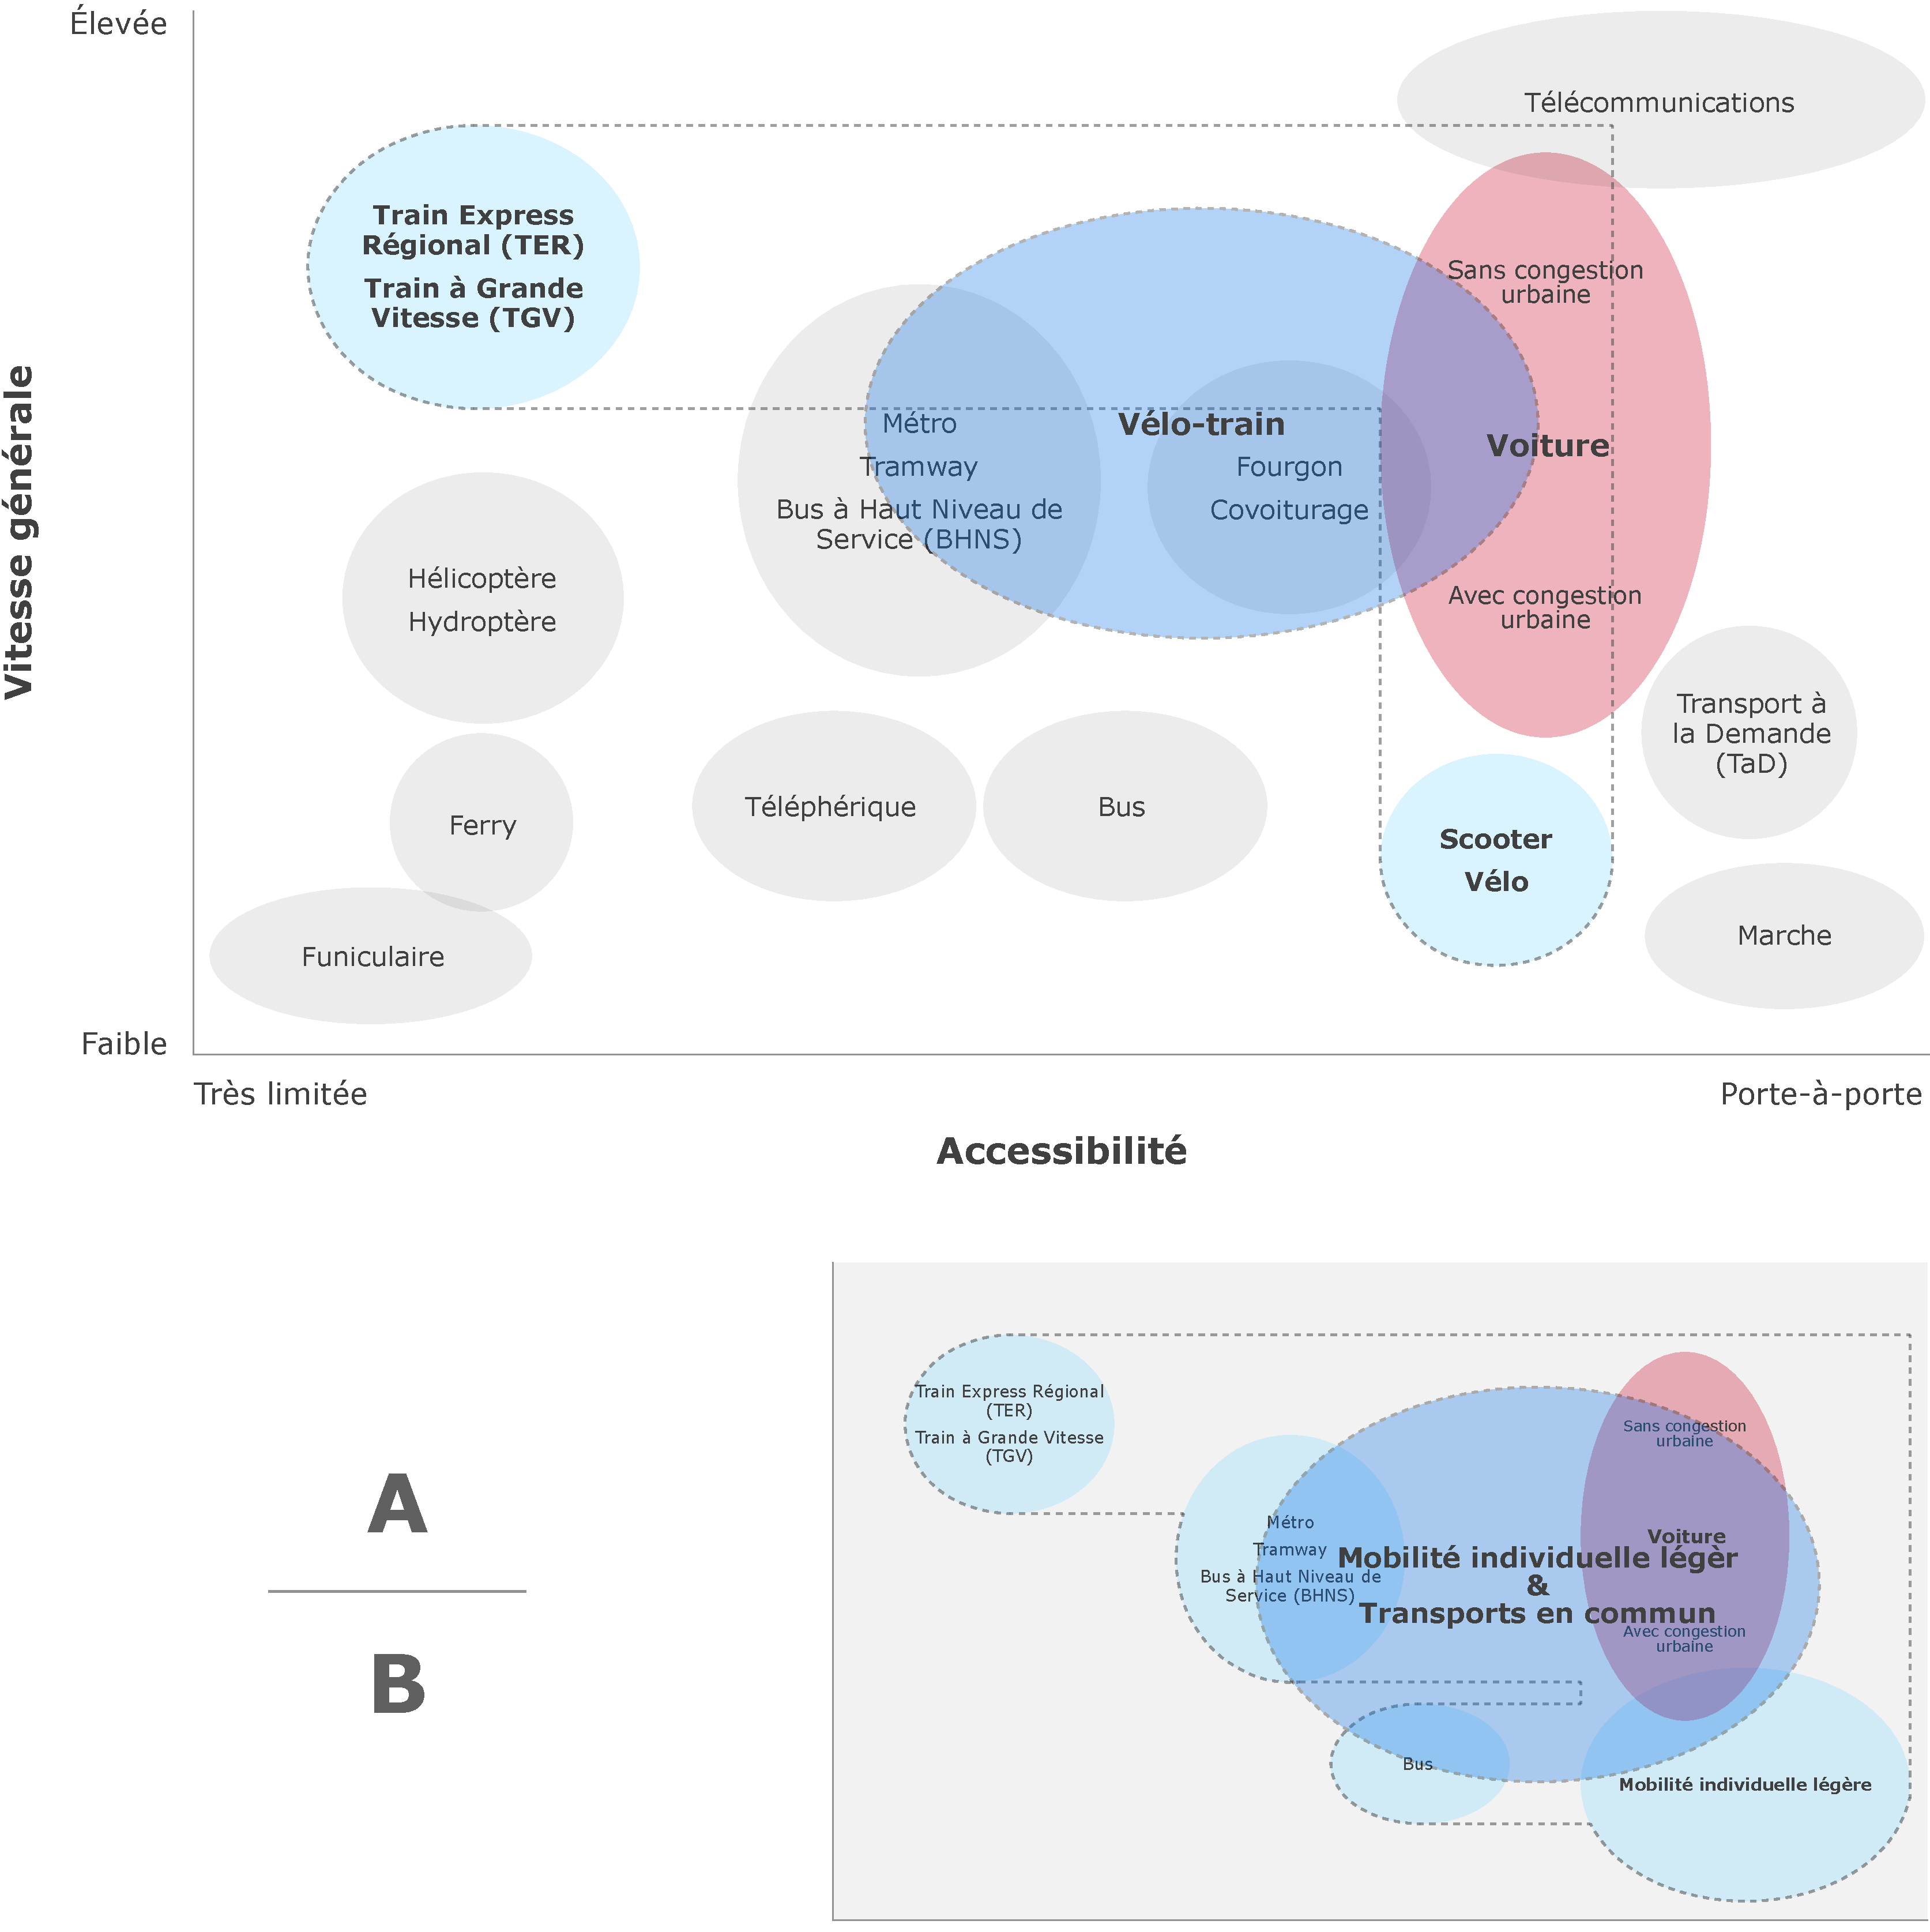
\includegraphics[width=1\columnwidth]{src/Figures/Chap-1/FR_Kager_vitesse_accessibilite.pdf}}
        \vspace{5pt}
        \begin{flushright}\scriptsize{
        Source (A)~: \textcolor{blue}{\textcite[212]{kager_characterisation_2016}}\index{Kager, Roland|pagebf}\index{Bertolini, Luca|pagebf}\index{te Brömmelstroet, Marco|pagebf}
        \\
        Adaptation graphique et réinterprétation (B)~: \textcolor{blue}{Dylan Moinse (2025)}
        }\end{flushright}
    \end{figure}

    % Micro-mobilité
Tandis que le vélo est si bien intégré au \Guillemets{système train} aux Pays-Bas qu’un véritable mode de déplacement \textcolor{blue}{\autocite[129-148]{bruntlett_curbing_2020}}\index{Bruntlett, Melissa|pagebf}\index{Bruntlett, Chris|pagebf}, bimodal et appelé \Guillemets{vélo-train}, a émergé \textcolor{blue}{\autocite[112]{oosteren_pourquoi_2021}}\index{Oosteren, Stein van|pagebf}\index{Schneider, Olivier|pagebf}, qu’en est-il de la micro-mobilité~? Il apparaît que cette famille d'engins de déplacement remplit une fonction et possède des propriétés proches de celles du vélo. En effet, les \acrshort{EDP} offrent un potentiel comparable pour accroître la portée de la marche, permettant de couvrir des distances deux à trois fois plus longues avec une vitesse de déplacement environ trois fois plus élevée \textcolor{blue}{\autocite{rabaud_micromobilites_2019}}\index{Rabaud, Mathieu|pagebf}\index{Richer, Cyprien|pagebf}. Ainsi, la micro-mobilité contribue, à son tour, à la redéfinition des aires de chalandise du transport public, en facilitant l’accès aux stations et en élargissant leur zone d’influence. Un avantage spécifique des \acrshort{EDP} réside cependant dans leur compacité et leur légèreté, qui favorisent leur embarquement dans le mode collectif, contrairement au vélo classique (voir le \hyperref[fig-chap1:vitesse-accessibilite-velo-tc]{diagramme~\ref{fig-chap1:vitesse-accessibilite-velo-tc}}, page~\pageref{fig-chap1:vitesse-accessibilite-velo-tc}). Dès lors, qu’il s’agisse du vélo ou des engins de micro-mobilité, ces modes répondent à des attentes et à des besoins similaires~: la recherche de gains de flexibilité et un accès direct et plus souple aux nœuds compatibles avec les enjeux d'ordre environnemental \textcolor{blue}{\autocite[80]{oostendorp_combining_2018}}\index{Oostendorp, Rebekka|pagebf}\index{Gebhardt, Laura|pagebf}.%%Rédigé%%

    % Impacts + Transition
Les atouts du couple mobilité individuelle légère et transports en commun, dont l’augmentation des distances que les usager·ère·s sont prêt·e·s à parcourir pour rejoindre ou quitter une station de transport public, participeraient à une hausse significative de la fréquentation du réseau \textcolor{blue}{\autocite[]{wang_approximating_2016}}\index{Wang, Hai|pagebf}\index{Odoni, Amedeo|pagebf}. Une modélisation réalisée par \textcolor{blue}{\textcite[69]{ensor_mode_2021}}\index{Ensor, Matt|pagebf}\index{Maxwell,~O.|pagebf}\index{Bruce, Oliver|pagebf} montre ainsi que l’essor de la pratique du vélo et de la \acrshort{TEP} pourrait conduire à une augmentation de 7~\% de la fréquentation des transports en commun en milieu urbain, et de 9~\% en territoire \gls{périurbain}, en Nouvelle-Zélande, si les configurations intermodales sont optimisées. Ce constat souligne un point clé~: bien que le vélo et la micro-mobilité ne soient pas en mesure d’être intégralement compétitifs face à l’automobile sur de longues distances et qu’ils aient une capacité limitée à s’y substituer, leur intégration au transport public crée une synergie qui les rend fortement concurrentiels vis-à-vis de ce mode de déplacement \textcolor{blue}{\autocite[43]{corporate_partnership_board_good_2020}}\index{Corporate Partnership Board@\textsl{Corporate Partnership Board}|pagebf}. Comme l’explique \textcolor{blue}{Annie-Claude} \textcolor{blue}{\textcite[262]{sebban_complementarite_2003}}\index{Sebban, Annie-Claude|pagebf}\index{Motte, Alain|pagebf}, l’intermodalité vélo et transport public se structure à travers des \textsl{territoires de pratique}. Cette approche lui permet de mobiliser la notion de territoire, dans la mesure où ces pratiques intermodales s’opèrent \textsl{sur} et \textsl{entre} des espaces bien déterminés. Envisager l’intermodalité sous l’angle territorial nous conduit naturellement à un retour au modèle du \acrshort{TOD}. Celui-ci apparaît comme un cadre pertinent à revisiter au regard des défis liés aux \Guillemets{premiers et derniers kilomètres}, auxquels la mobilité individuelle légère semble particulièrement adaptée.%%Rédigé%%

    % 1.3.2.2.
    \needspace{1\baselineskip} % Réserve de l'espace
\subsubsection*{Conceptualisation d'un urbanisme orienté vers le rail et soutenu par la mobilité individuelle légère
    \label{chap1:btod-m-tod}
    }

    % Introduction aires secondaires
Dans leur ouvrage proposant un regard contemporain sur le \acrshort{TOD}, \foreignlanguage{english}{\textsl{Transit-Oriented Development and Sustainable Cities: Economics, Community and Methods}}, \textcolor{blue}{\textcite[222]{knowles_transit_2019}}\index{Knowles, Richard~D.|pagebf}\index{Ferbrache, Fiona|pagebf} soulignent l’importance de tirer parti des opportunités offertes par les mobilités émergentes de ces dernières années~–~telles que le \acrshort{VAE}, la \acrshort{TEP} et les services en \textsl{free-floating}~–~afin d’enrichir le modèle urbain du \acrshort{TOD}. \textcolor{blue}{Peter} \textcolor{blue}{\textcite[54-55]{calthorpe_next_1993}}\index{Calthorpe, Peter|pagebf} n’abandonne pas pour autant la prise en compte des \Guillemets{aires secondaires} dans la structuration des quartiers \acrshort{TOD}\textcolor{blue}{s}. Il les intègre partiellement au \acrshort{TOD}, considérant qu’elles sont suffisamment proches d’une station de transport en commun pour être orientées vers celle-ci, notamment grâce à un accès cyclable. L'\Guillemets{aire secondaire} détient même des caractéristiques semblables à celles de l’\Guillemets{aire primaire} en bénéficiant d'une certaine diversité fonctionnelle et en étant connectée à un réseau de rues apaisées. Loin d’être marginale, cette aire joue un rôle structurant dans chaque quartier de gare. Elle accueille généralement des fonctions rarement configurées pour être placée dans l’aire la plus stratégique, telles que des emplois en dehors des bureaux, des écoles ou encore des parcs. Elle permet également d’offrir une diversité en termes de choix résidentiel, en intégrant plus souvent des maisons individuelles. L'auteur identifie trois types d’\Guillemets{aires secondaires}~: (i) celles séparées par une artère, mais proches d’un arrêt de transport en commun~; (ii) celles séparées par une artère et éloignées de l’arrêt~; (iii) et celles plus éloignées encore de l’arrêt, mais sans artère séparatrice \textcolor{blue}{\autocite[87]{calthorpe_next_1993}}\index{Calthorpe, Peter|pagebf}. Bien que l'\Guillemets{aire secondaire} soit souvent plus auto-orientée et accueille fréquemment des infrastructures de type \acrfull{P+R} favorisant la pratique du \textsl{park-and-ride}, elle devrait selon lui être desservie par des connexions cyclables la reliant directement à la station de transport en commun et au quartier de gare central. Dès la formalisation du \acrshort{TOD}, l’enjeu majeur réside dans la maximisation des connexions piétonnes et, surtout, cyclables au sein de l’\Guillemets{aire secondaire}. Il préconise en particulier l’aménagement de pistes cyclables séparées le long des boulevards urbains structurants\footnote{
    \Guillemets{\textsl{En raison des distances, le vélo est l’un des modes de déplacement les plus probables pour les résidents des zones secondaires susceptibles d’utiliser les transports en commun. Des connexions cyclables solides empruntant les itinéraires les plus courts possibles encourageront davantage les résidents des zones secondaires à utiliser les transports en commun. Les artères et certaines voies de connexion dans les zones secondaires doivent offrir des pistes cyclables sécurisées, séparées ou marquées, permettant un accès rapide à l’arrêt de transport en commun. Les pistes cyclables des zones secondaires devraient se connecter au réseau cyclable du TOD.}} (\Guillemets{\textsl{Because of the distances, bicycles are one of the most likely modes of travel for Secondary Area residents who are apt to use public transit. Strong bicycle connections that follow the shortest possible routes will provide additional encouragement for Secondary Area residents to use transit. Arterials and selected connector roadways in Secondary Areas must provide safe, separated or marked bicycle lanes allowing quick travel to the transit stop. Secondary Area bicycle paths should connect with the TOD bicycle system}}) \textcolor{blue}{\autocite[89]{calthorpe_next_1993}}\index{Calthorpe, Peter|pagebf}.
} \textcolor{blue}{\autocite[60, 89]{calthorpe_next_1993}}\index{Calthorpe, Peter|pagebf}. Outre ces aménagements, l’auteur insiste sur l’importance du stationnement sécurisé pour vélo afin de favoriser leur usage intermodal, ainsi que sur le rôle du vélo dans les déplacements internes au quartier de gare\footnote{
    \Guillemets{\textsl{Des casiers sécurisés pour vélos sont particulièrement importants pour l’utilisation combinée \Guillemets{vélo-et-transports en commun}, car peu de personnes laisseront leur vélo sans surveillance pendant une journée entière de travail. Les infrastructures de stationnement pour vélos incluent des arceaux, des consignes surveillées et des casiers. Des arceaux à vélo doivent être installés à proximité des destinations commerciales, scolaires et de loisirs dans les TODs et les zones secondaires. Des installations de stationnement pour vélo plus sécurisées doivent être prévues à proximité de tous les bureaux, des lieux d’emploi et des principaux arrêts de transport en commun.}} (\Guillemets{\textsl{Secure bike lockers are especially important to "bike-and-ride" transit use, as few will leave their bike unattended for a full working day. Bicycle parking facilities include bike racks, "checks", and lockers. Bike racks must be provided at shopping, school, and recreational destinations in TODs and Secondary Areas. More secure bike parking facilities must be provided at all office/employment uses and at major transit stops.}}) \textcolor{blue}{\autocite[103]{calthorpe_next_1993}}\index{Calthorpe, Peter|pagebf}.
} \textcolor{blue}{\autocite[103]{calthorpe_next_1993}}\index{Calthorpe, Peter|pagebf}. Plus qu’une simple connexion au réseau structurant, il s’agit de proposer un maillage cyclable capillaire permettant d’accéder à l’ensemble des aménités présentes dans le quartier de gare~–~qu’elles soient situées dans l’aire primaire ou secondaire~–~et de relier efficacement un \acrshort{TOD} à un autre\footnote{
    \Guillemets{\textsl{Un réseau coordonné de voies cyclables devrait être mis en place en lien avec les TOD ou une série de TOD. Des destinations importantes, telles que les zones commerciales centrales, les arrêts de transport en commun, les centres d’emploi, les parcs, les espaces ouverts, les écoles et autres équipements communautaires, devraient être reliées par ces itinéraires cyclables.} [\dots] \textsl{Des pistes cyclables séparées ou marquées sur plusieurs axes principaux menant au centre favoriseront cette alternative, tout comme les voies cyclables le long des corridors verts reliant les TOD aux destinations professionnelles. Sur les rues secondaires, le partage de la chaussée entre vélos et voitures contribuera à réduire la vitesse des véhicules à des niveaux plus adaptés aux rues résidentielles. Certains itinéraires menant aux arrêts de transport en commun devraient offrir des pistes cyclables marquées ou séparées, connectées aux zones secondaires et à d'autres destinations clés. Des voies cyclables désignées devraient être prévues sur certaines rues de connexion et un nombre limité de rues locales convergeant vers le centre commercial et de transport.} [\dots] \textsl{Des panneaux clairs indiquant les destinations principales devraient être installés pour guider les cyclistes vers les principaux pôles d’activité, tels que les zones commerçantes, les arrêts de transport, les équipements de loisirs, les écoles et les infrastructures de stationnement pour vélos.}} (\Guillemets{\textsl{A coordinated system of bikeways should be provided in conjunction with TODs or a series of TODs. Important destinations, such as core commercial areas, transit stops, employment centers, parks, open spaces, schools, and other community facilities, should be linked by these bike routes.} [\dots] \textsl{Separated or marked bike lanes on several primary routes to the core area will support this alternative, as will the bike paths along greenways between TODs and employment destinations. On smaller streets, bikes sharing the travel lane will help slow cars to speeds more appropriate for residential streets. Selected routes to the transit stop should provide marked or separated bikeways connecting with the Secondary Areas and other key destinations. Designated bike lanes should be provided on selected connector streets and a limited number of local streets that converge upon the commercial and transit center.} [\dots] \textsl{Clear destination signs should be provided that direct riders to key activity centers, such as shopping areas, transit stops, recreation facilities, schools, and bike parking facilities.}}) \textcolor{blue}{\autocite[102]{calthorpe_next_1993}}\index{Calthorpe, Peter|pagebf}.
} \textcolor{blue}{\autocite[102]{calthorpe_next_1993}}\index{Calthorpe, Peter|pagebf}. Ainsi, au regard des avantages comparatifs liés à l’intégration de la mobilité individuelle légère au réseau de transport public, l’enjeu dépasse la seule \Guillemets{poche piétonnière} pour viser une intégration complète de l’\Guillemets{aire secondaire} au sein du \acrshort{TOD} \textcolor{blue}{\autocite[112]{ibraeva_transit-oriented_2020}}\index{Ibraeva, Anna|pagebf}\index{Almeida Correia, Gonçalo Homem de|pagebf}\index{Silva, Cecília|pagebf}.%%Rédigé%%

    % Figure B-TOD
    \begin{carte}[h!]\vspace*{4pt}
        \caption{Configurations spatiales du \textsl{Bicycle-based Transit-Oriented Development}.}
        \label{fig-chap1:schema-b-tod}
        \centerline{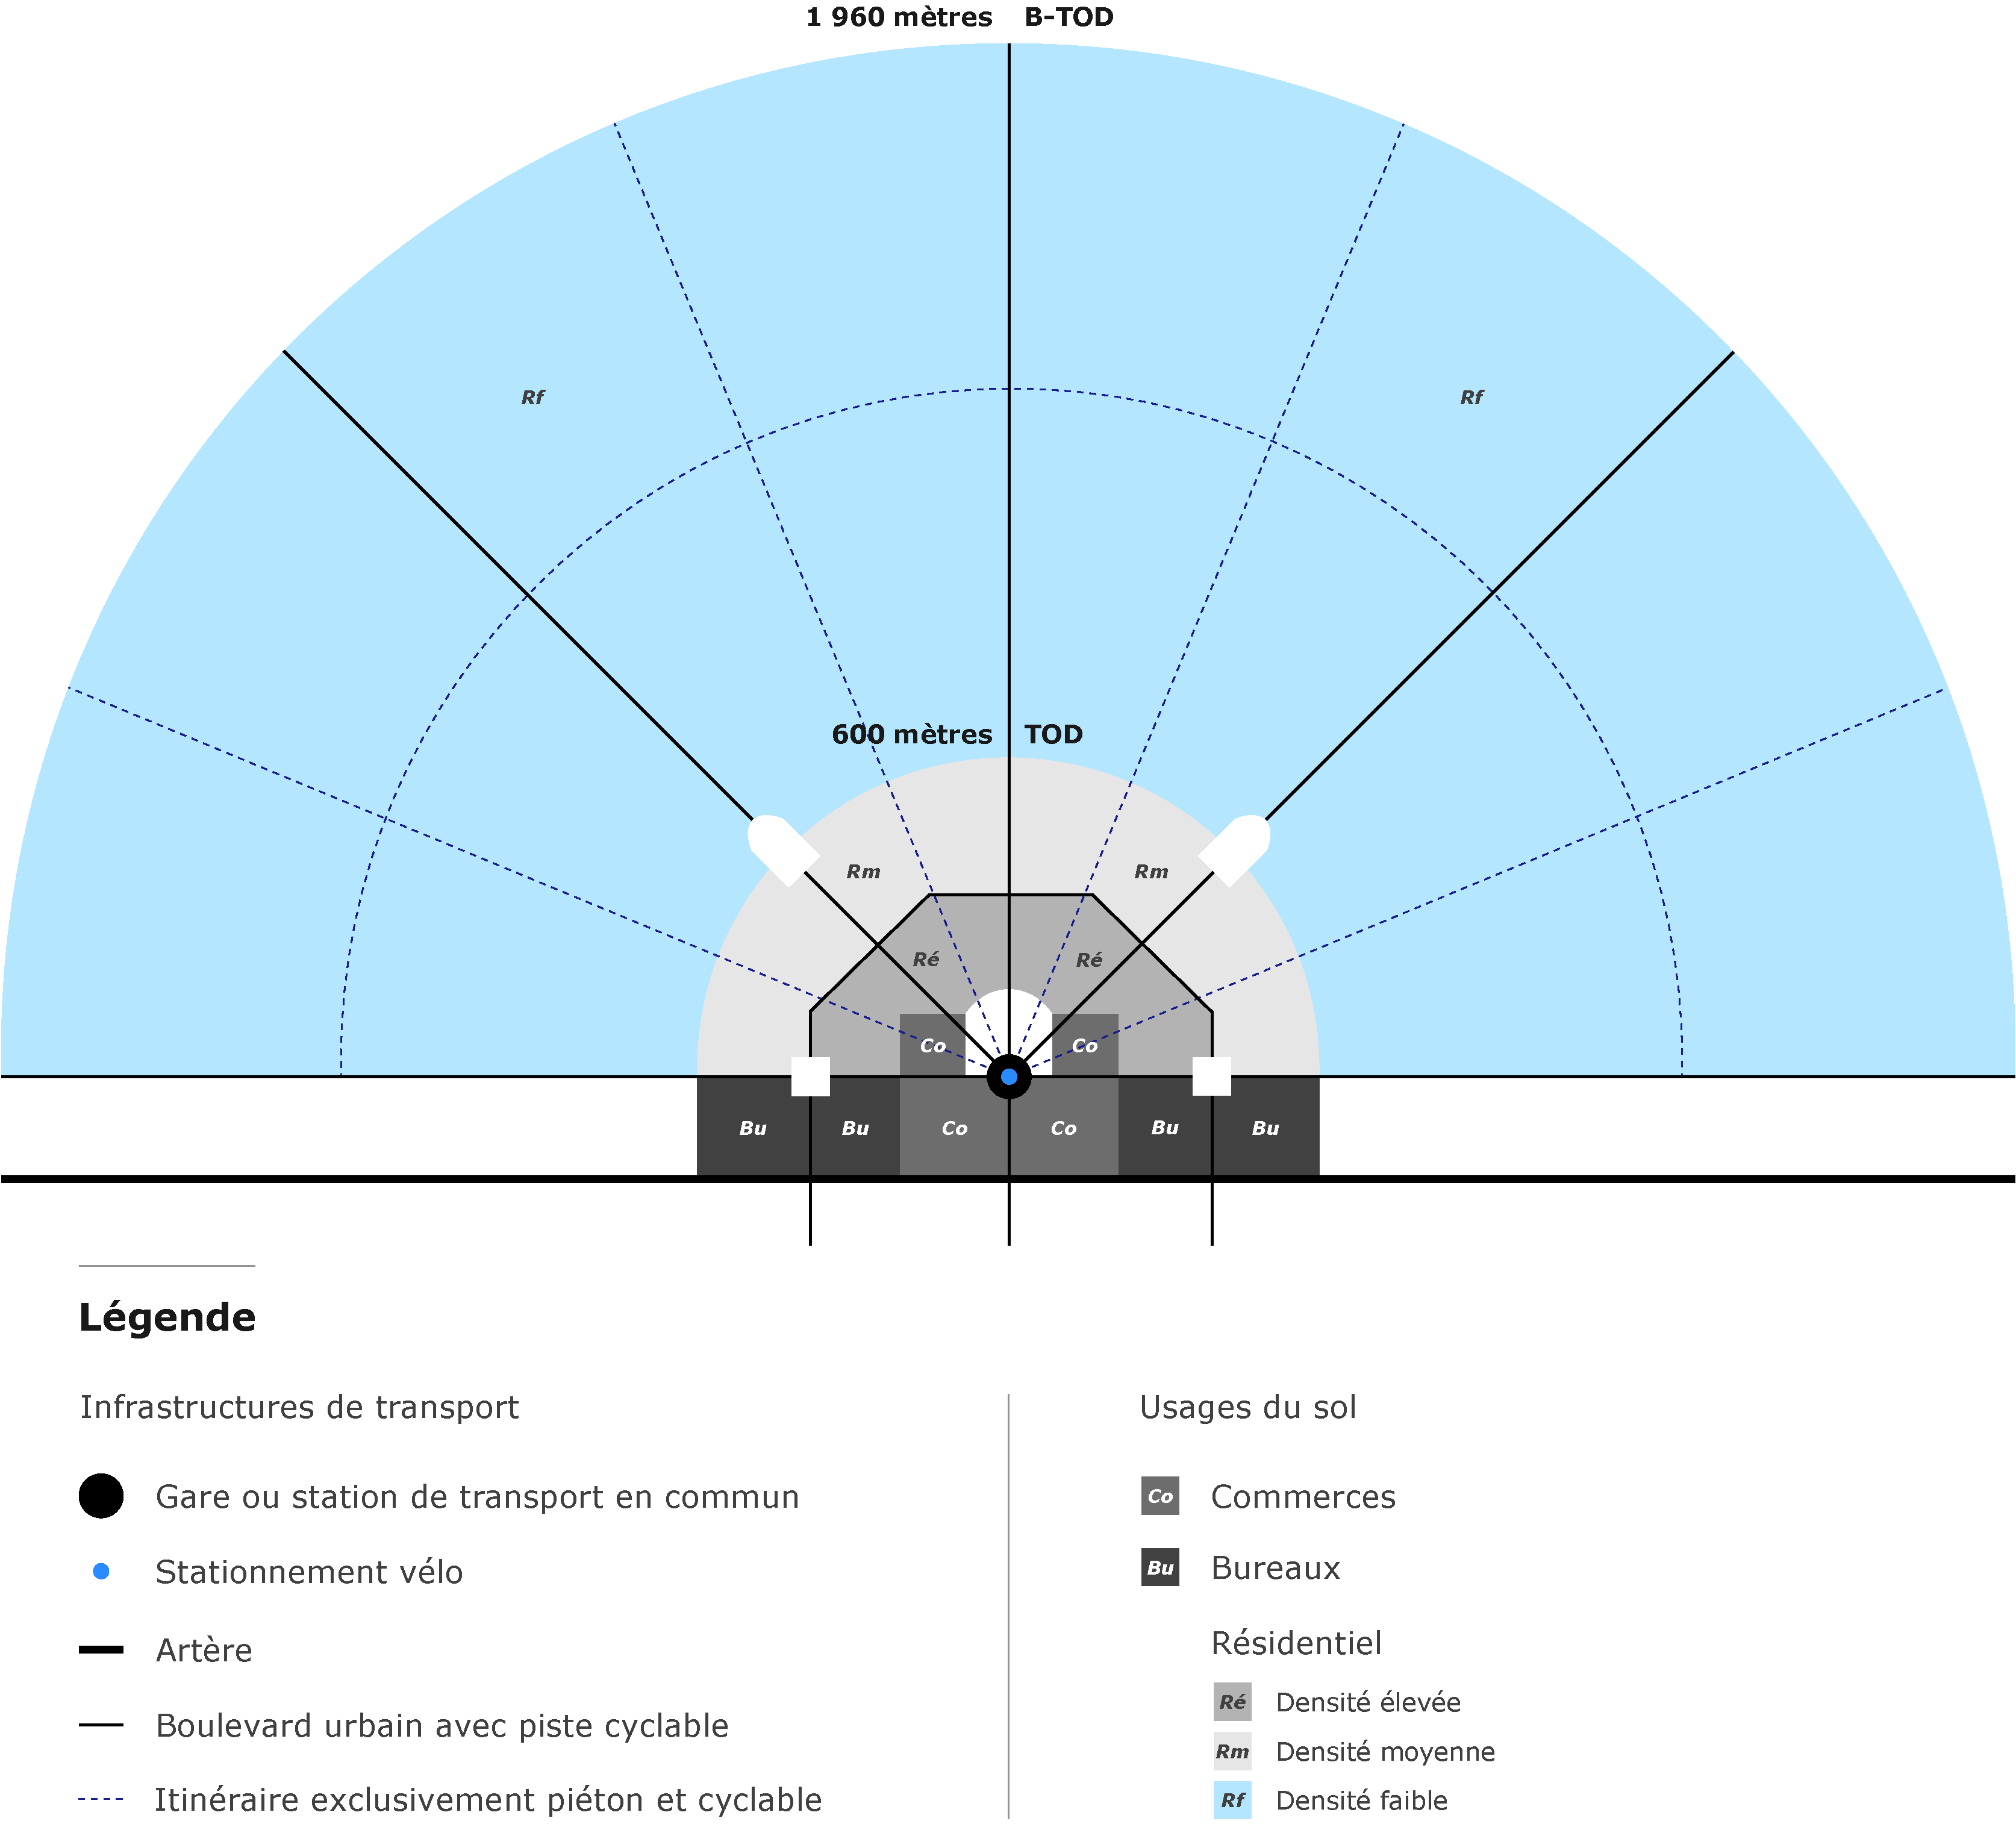
\includegraphics[width=1\columnwidth]{src/Figures/Chap-1/FR_Schema_B_TOD.pdf}}
        \vspace{5pt}
        \begin{flushright}\scriptsize{
        Source~: \textcolor{blue}{\textcite[979]{lee_bicycle-based_2016}}\index{Lee, Jaeyeong|pagebf}\index{Choi, Keechoo|pagebf}\index{Leem, Yountaik|pagebf}
        \\
        Adaptation graphique~: \textcolor{blue}{Dylan Moinse (2024)}
        }\end{flushright}
    \end{carte}

    % B-TOD
Bien que la problématique des \Guillemets{premiers et derniers kilomètres} et la solution intermodale associée à la pratique du vélo aient été envisagées dès l’ouvrage fondateur du \acrshort{TOD}, il apparaît que les développements relatifs à l’\Guillemets{aire secondaire} et aux aménagements cyclables proposés ont progressivement perdu en visibilité et en clarté dans les principes édictés. Face à cette appropriation partielle, les chercheur·se·s sud-coréen·ne·s \textcolor{blue}{\textcite[979]{lee_bicycle-based_2016}}\index{Lee, Jaeyeong|pagebf}\index{Choi, Keechoo|pagebf}\index{Leem, Yountaik|pagebf}, dans leur article \textsl{Bicycle-based transit-oriented development as an alternative to overcome the criticisms of the conventional transit-oriented development}, proposent, deux décennies plus tard, la conceptualisation d’un \acrfull{B-TOD} (voir la \hyperref[fig-chap1:schema-b-tod]{carte~\ref{fig-chap1:schema-b-tod}}, page~\pageref{fig-chap1:schema-b-tod}). Cette déclinaison du \acrshort{TOD}, qui ne remet pas en cause les principes fondamentaux du modèle, vise à répondre aux besoins de territoires n’ayant pas atteint les seuils critiques de densité de population et d’emploi nécessaires pour maximiser leur demande en transport autour des stations. Le \acrshort{B-TOD} cherche ainsi à accroître la fréquentation du réseau de transport en commun en ciblant les aires d’influence accessibles à vélo, définies dans un rayon d’environ deux kilomètres \textcolor{blue}{\autocite[979]{lee_bicycle-based_2016}}\index{Lee, Jaeyeong|pagebf}\index{Choi, Keechoo|pagebf}\index{Leem, Yountaik|pagebf}. Ce modèle revisité présente d'autres avantages notables. Il permet d’étendre jusqu'à 25 fois la superficie du quartier de gare traditionnel, renforçant ainsi considérablement son potentiel d’attractivité. De plus, avec une mise en œuvre facilitée, il se positionne comme une alternative écologique aux modèles du \acrshort{TOD} et du \acrshort{E-TOD}, tout en nécessitant un investissement infrastructurel réduit \textcolor{blue}{\autocite[979, 983]{lee_bicycle-based_2016}}\index{Lee, Jaeyeong|pagebf}\index{Choi, Keechoo|pagebf}\index{Leem, Yountaik|pagebf}, comme nous l’avons évoqué dans la \hyperref[chap1:tod-presentation-generale-declinaisons-hybrids]{sous-section sur les déclinaisons du \textsl{Transit-Oriented Development}} (page~\pageref{chap1:tod-presentation-generale-declinaisons-hybrids}). Un quatrième avantage, moins explicitement formulé par les auteur·rice·s, vaut la peine d'être signalé, à nos yeux~: le \acrshort{B-TOD} permettrait une adaptation des \Guillemets{[\dots] \textsl{critères de densité de population qui serait plus ou moins assouplis, par rapport à ceux de la zone centrale, afin de préserver un cadre plus agréable dans cette zone.}}\footnote{
    \Guillemets{\textsl{In a B-TOD setting, the re-establishment of the station impact area, where bicycle is a main access mode should be identified and the density criteria could be more or less relaxed than that of a TOD to keep the station impact area more pleasant.}} \textcolor{blue}{\autocite[983]{lee_bicycle-based_2016}}\index{Lee, Jaeyeong|pagebf}\index{Choi, Keechoo|pagebf}\index{Leem, Yountaik|pagebf}.
} \textcolor{blue}{\autocite[983]{lee_bicycle-based_2016}}\index{Lee, Jaeyeong|pagebf}\index{Choi, Keechoo|pagebf}\index{Leem, Yountaik|pagebf}. Toutefois, il ne s’agit pas de réduire la densité, mais plutôt de mieux la répartir au sein de l’aire du \acrshort{B-TOD}, en offrant des opportunités résidentielles pour des individus à la recherche de territoires moins denses, mieux dotés en espaces verts, offrant un accès facilité à des logements familiaux ou permettant d’échapper à la pression foncière autour des centralités. Afin de valider leur exercice de conceptualisation, les auteur·rice·s ont mené une enquête auprès des \Guillemets{cyclo-voyageur·se·s}~–~c’est l'expression que nous privilégions pour désigner les usager·ère·s combinant vélo et transport public lors d’un même déplacement~–~dans les villes de Séoul et Daejeon. Leur modélisation montre que 94~\% de l’aire métropolitaine de Séoul pourrait devenir accessible en transport en commun grâce à l’usage intermodal du vélo, soit une couverture potentielle trois fois supérieure à celle permise par la marche combinée \textcolor{blue}{\autocite[982]{lee_bicycle-based_2016}}\index{Lee, Jaeyeong|pagebf}\index{Choi, Keechoo|pagebf}\index{Leem, Yountaik|pagebf}. Réorganiser l'urbanisme autour du transport public et du vélo revient non seulement à promouvoir l'écologie, mais surtout la santé et l'activité physique \textcolor{blue}{\autocite[44]{heran_velo_2020}}\index{Héran, Frédéric|pagebf}\index{Rymarski, Christophe|pagebf}\index{Bedin, Véronique|pagebf}, une dimension moins abordée dans le \acrshort{TOD} conventionnel.%%Rédigé%%

    % M-TOD
Fort de cette déclinaison, nous avons fait le choix de nous appuyer sur ce travail de recherche, qui nous paraît fondateur, afin d’en tirer inspiration et de transposer notre argumentaire développé tout au long de ce chapitre. Il s’agit, en particulier, de démontrer le potentiel de la mobilité individuelle légère à renforcer le modèle urbain du \acrshort{TOD}, dans une perspective de promotion d’une mobilité et d’un cadre urbain plus soutenables. En nous inspirant des arguments avancés par \textcolor{blue}{\textcite{lee_bicycle-based_2016}}\index{Lee, Jaeyeong|pagebf}\index{Choi, Keechoo|pagebf}\index{Leem, Yountaik|pagebf}, et en reprenant notamment leurs questionnements autour de l’\Guillemets{identification} et de la \Guillemets{définition} d’un \acrshort{B-TOD}, nous proposons une réactualisation de ces modèles afin d’en concevoir un \acrfull{M-TOD}. Finalement, nous pourrions transposer la proposition de \Guillemets{théorie générale de la marchabilité} formulée par l’urbaniste \textcolor{blue}{Jeff} \textcolor{blue}{\textcite[73]{speck_walkable_2013}}\index{Speck, Jeff|pagebf} vers une \Guillemets{théorie générale de la cyclabilité} articulée autour du système de transport public. Celle-ci intégrerait l’ensemble de la mobilité individuelle légère et remplirait, à l’instar de la marchabilité, une triple fonction~: celle d’une finalité en soi, d’un moyen d’accessibilité et d’une mesure de la qualité urbaine \textcolor{blue}{\autocite[73]{speck_walkable_2013}}\index{Speck, Jeff|pagebf}. Dès lors, plusieurs interrogations structurent, à ce stade, notre réflexion~:
    \begin{customitemize}
\item Qu’est-ce qu’un \acrshort{M-TOD} et en quoi se distingue-t-il d’un \acrshort{TOD} et d’un \acrshort{B-TOD}~?
\item Quels en sont les usages observables et quel est son potentiel de report modal~?
\item Quels sont les liens entre le transport public et la mobilité individuelle légère~?
\item Comment ces comportements de mobilité actuels et potentiels interagissent-ils avec le tissu urbain et les enjeux de développement territorial~?
    \end{customitemize}%%Rédigé%%

    % ___________________________________________
    % 1.*.
    \newpage
    \needspace{1\baselineskip} % Réserve de l'espace
    \addcontentsline{toc}{section}{Conclusion du chapitre~1}
    \sectionheader{Conclusion du chapitre}
\section*{Conclusion du chapitre~1
    \label{chap1:conclusion}
    }
    %\markright{Conclusion du chapitre~1}{}

    % Introduction
Le \acrfull{TOD} constitue aujourd’hui un levier stratégique d'une planification urbaine soutenable, offrant une réponse aux défis posés par les politiques du \Guillemets{partout automobile} et du \Guillemets{surtout automobile}, qui continuent d’orienter la fabrique urbaine en France \textcolor{blue}{\autocite[14]{sebban_complementarite_2003}}\index{Sebban, Annie-Claude|pagebf}\index{Motte, Alain|pagebf}. Ce chapitre a permis de revenir sur les fondements historiques, les principes directeurs et les déclinaisons contemporaines de ce modèle d’aménagement. Bien que sa formalisation ait émergé dans le contexte nord-américain, il serait erroné d’en attribuer exclusivement la paternité aux urbanistes étasunien·ne·s, celleux-ci reconnaissant elleux-mêmes s’être inspiré·e·s d’exemples européens \textcolor{blue}{\autocite[15]{renne_emerging_2004}}\index{Renne, John Luciano|pagebf}\index{Wells, J.~S.|pagebf}. En somme, le cadre théorique et opérationnel du \acrshort{TOD} constitue une base solide et pertinente pour répondre aux impératifs environnementaux et socio-économiques actuels, à la fois à l’échelle régionale et locale. Il ne s’agit pas uniquement de promouvoir une meilleure offre de transport en commun~–~bien que cela soit une condition nécessaire~–, mais d’inscrire cette offre dans une logique d’interaction avec la structuration territoriale \textcolor{blue}{\autocite[9]{bernier_atlas_2023}}\index{Bernier, Xavier|pagebf}, en suivant une dynamique de \Guillemets{congruence}\footnote{
    Dans son article intitulé \textsl{Les \Guillemets{effets structurants} du transport~: mythe politique, mystification scientifique}, \textcolor{blue}{Jean-Marc} \textcolor{blue}{\textcite[239]{offner__1993}}\index{Offner, Jean-Marc|pagebf} a remarquablement exposé la nécessité d’une \Guillemets{démystification} politico-médiatique et scientifique concernant l’évaluation et les attentes suscitées par les \Guillemets{effets structurants} des infrastructures de transport. Il remet en question l’idée d’une relation de causalité linéaire entre l’introduction d’une nouvelle offre de mobilité et le développement territorial, en mettant en évidence une dynamique pré-existante plus complexe de liens parallèles, qu’il qualifie de \Guillemets{congruence}.
}, concept développé par \textcolor{blue}{Jean-Marc} \textcolor{blue}{\textcite[239]{offner__1993}}\index{Offner, Jean-Marc|pagebf}. La finalité du \acrshort{TOD} n’est donc pas tant de \Guillemets{générer de la croissance} (économique, démographique ou urbaine) en valeur absolue, mais plutôt de la redistribuer de manière plus équilibrée au sein d’une région donnée \textcolor{blue}{\autocite[82]{cervero_transit_1998}}\index{Cervero, Robert|pagebf}.%%Rédigé%%

    % Forces du TOD
L’intérêt principal des quartiers \acrshort{TOD}\textcolor{blue}{s} ne tient pas uniquement à leur aptitude à attirer une nouvelle clientèle vers le transport public, mais également à leur capacité à produire des environnements urbains agréables à vivre et à fréquenter, caractérisés par leur densité et leur convivialité \textcolor{blue}{\autocite[40]{bentayou_transit-oriented_2015}}\index{Bentayou, Gilles|pagebf}. En définitive, cette stratégie d’aménagement s’inscrit pleinement dans le troisième scénario prospectif étudié par la SNCF\footnote{
    L’étude commandée par la SNCF explore les évolutions possibles de la mobilité des personnes en France à l’horizon 2050 ainsi que leurs implications environnementales et sociales. Prenant appui sur les réflexions d’expert·e·s français·es et internationaux·les, elle s’appuie également sur les résultats d’une enquête menée par l’\acrfull{IFOP} en 2015 auprès de 1~800 Français·es. Trois scénarios prospectifs y sont dégagés, en fonction des dynamiques d’évolution de la demande de mobilité et de l’offre de transport~: (i) l'\Guillemets{ultramobilité~: toujours plus vite, toujours plus loin}~; (ii) l'\Guillemets{altermobilité~: se déplacer autrement}~; et (iii) la \Guillemets{proximobilité~: la qualité de vie de la proximité} qui incorpore l'\Guillemets{altermobilité}. Parmi ces scénarios, seul le dernier permettrait d’atteindre l’objectif national de réduction des émissions de \acrfull{GES} d’un facteur quatre (\textsl{Facteur~4}), tout en générant une économie annuelle de 100 milliards d’euros pour la collectivité, en comparaison avec la situation actuelle et les deux autres trajectoires envisagées \textcolor{blue}{\autocite[26-37]{sncf_vers_2015}}.
}, celui de la \Guillemets{proximobilité}, qui repose sur la mise en place d’un système de mobilité alternative à l’automobile (\Guillemets{altermobilité}) en cohérence avec une reconfiguration territoriale favorisant un meilleur ancrage local, le développement des modes actifs et la densification urbaine \textcolor{blue}{\autocite[26-37]{sncf_vers_2015}}\index{SNCF@\textsl{SNCF}|pagebf}. Ce scénario apparaît d’ailleurs comme le seul à même d’atteindre l’objectif de réduction des émissions de \acrfull{GES} d’un facteur quatre d’ici à 2050, en veillant à articuler efficacement le système de transport, l’organisation urbaine et les micro-circulations au sein des quartiers de gare \textcolor{blue}{\autocite[148]{krakovitch_metropolitrain_2019}}\index{Krakovitch, Alain|pagebf}. En d’autres termes, seule une refonte en profondeur de l’organisation territoriale permettra d’\Guillemets{arracher l’automobile à la ville} \textcolor{blue}{\autocite[184]{ducharme_ville_2021}}\index{Ducharme, Olivier|pagebf}.%%Rédigé%%

    % Micro-mobilité
L’imbrication de la mobilité individuelle légère dans le cadre du \acrshort{TOD} défend un positionnement qui vient en appui au réseau de transport public, de manière à renforcer l’efficacité globale du système de mobilité alternatif et à contribuer à l’émergence d'une \Guillemets{sobriété énergétique} ou d'une \Guillemets{ville post-carbone} \textcolor{blue}{\autocite[2]{schultz_micromobility_2019}}\index{Schultz, Stéphane|pagebf}\index{Grisot, Sylvain|pagebf}. Portée par l’essor de nouvelles formes de déplacement, par l’électromobilité et par le développement des services de partage, avec ou sans borne d'attachement, la mobilité individuelle légère répond à des besoins émergents qui dépassent la dichotomie traditionnelle entre véhicule personnel et transport collectif. Elle s’impose comme une solution pratique et flexible, permettant aux usager·ère·s de devenir de véritables \Guillemets{piéton·ne·s augmenté·e·s} \textcolor{blue}{\autocite[1]{boffi_extrait_2019}}\index{Boffi, Nicolas|pagebf}. Comme l’affirme le Secrétaire général de l’\acrfull{UITP}, la mobilité individuelle légère \Guillemets{ [\dots] \textsl{fait partie intégrante du transport public, car elle répond à des objectifs convergents, à savoir~: une meilleure utilisation de l’espace urbain, une réduction des émissions de polluants et de gaz à effet de serre~; de plus} [\dots] [elle] \textsl{peut être facilement combinée avec le transport public traditionnel~–~aussi bien physiquement qu’en termes de services et de tarification} [\dots]}\footnote{
    \Guillemets{[\dots] \foreignlanguage{english}{\textsl{micromobility is an integral part of public transport because it meets objectives that are also converging, namely: better use of urban space, less emissions of pollutants and greenhouse gases; plus micromobility modes can be easily combined with traditional public transport~–~both physically and in terms of services and fares}} [\dots]} \textcolor{blue}{\autocite{bcg_role_2020}}.
} \textcolor{blue}{\autocite{bcg_role_2020}}\index{BCG@\textsl{BCG}|pagebf}. Il convient alors de rappeler combien le \acrshort{TOD} demeure un modèle flexible, dont l’application varie selon les contextes et les problématiques spécifiques. Ses principes directeurs ne constituent pas un cadre rigide, mais bien un \textsl{ethos}, comme le souligne \textcolor{blue}{Peter} \textcolor{blue}{\textcite[11]{calthorpe_next_1993}}\index{Calthorpe, Peter|pagebf}. En ce sens, nous avons observé que les \textsl{Transit Metropolises} ont évolué ces dernières décennies en intégrant des approches hybrides, combinant des interventions sur l’offre et la demande de mobilité \textcolor{blue}{\textcite[137-143]{cervero_transit_2020}}\index{Cervero, Robert|pagebf}.%%Rédigé%%

    % B-TOD
Au-delà du simple développement de \Guillemets{véhicules intelligents}, la mobilité individuelle légère s’affirme comme un acteur qui vient d'abord optimiser l'\Guillemets{intelligence des flux, de l'espace et du réseau} dans lesquels ces véhicules s’insèrent \textcolor{blue}{\autocite[76]{krakovitch_metropolitrain_2019}}\index{Krakovitch, Alain|pagebf}. Son potentiel se révèle particulièrement dans la chaîne modale des déplacements, où elle renforce l’efficacité du transport public tout en proposant une alternative fluide et adaptable aux besoins de mobilité \textcolor{blue}{\autocite[4]{molino_pratiques_2015}}\index{Molino, Marie|pagebf}\index{Rampon, Anne-Sophie|pagebf}\index{Cipolla, Romain|pagebf}. Ce modèle \Guillemets{hybride}, à la fois performant, flexible et compétitif face à l’automobile \textcolor{blue}{\autocite[107]{wang_bicycle-transit_2013}}\index{Wang, Rui|pagebf}\index{Liu, Chen|pagebf}, évite l’écueil d’une expansion des marges de déploiement du système automobile, contrairement aux risques induits par la voiture autonome. Il propose au contraire un \Guillemets{bouquet d’offres} diversifié permettant de briser le \Guillemets{réflexe automobile} et de favoriser une transition vers des mobilités plus durables \textcolor{blue}{\autocites[81]{bertolini_planning_2017}[42]{6t-bureau_de_recherche_livre_2019}}\index{Bertolini, Luca|pagebf}\index{Bureau de recherche 6t@\textsl{Bureau de recherche 6t}|pagebf}. \textcolor{blue}{Annie-Claude} \textcolor{blue}{\textcite[35]{sebban_complementarite_2003}}\index{Sebban, Annie-Claude|pagebf}\index{Motte, Alain|pagebf} le présente de cette façon~: \Guillemets{\textsl{au lieu de se demander si la complémentarité entre vélo et transport public est défavorable à la circulation des véhicules de transport public, le problème ne devrait-il pas plutôt être posé dans les termes suivants~: la complémentarité entre vélo et transport public est-elle une pratique, voire une politique suffisamment défavorable au trafic automobile~?}}. Dans cette perspective, \textcolor{blue}{Georges} \textcolor{blue}{\textcite[225]{amar_homo_2016}}\index{Amar, Georges|pagebf} insiste sur la nécessité de créer des passerelles et des synergies entre les nouvelles formes de mobilité et les modèles d’urbanisme naissants. Les villes contemporaines doivent ainsi favoriser cette \Guillemets{reliance}, une approche que développent également \textcolor{blue}{\textcite[979]{lee_bicycle-based_2016}}\index{Lee, Jaeyeong|pagebf}\index{Choi, Keechoo|pagebf}\index{Leem, Yountaik|pagebf} à travers leur conceptualisation d'un \acrfull{B-TOD}.%%Rédigé%%

    % Figure Google scholar trends
    \begin{figure}[h!]\vspace*{4pt}
        \caption{Nombre de publications scientifiques internationales portant sur le \textsl{Transit-Oriented Development}, la micro-mobilité ou sur leur combinaison.}
        \label{fig-chap1:trends-google-scholar}
        \centerline{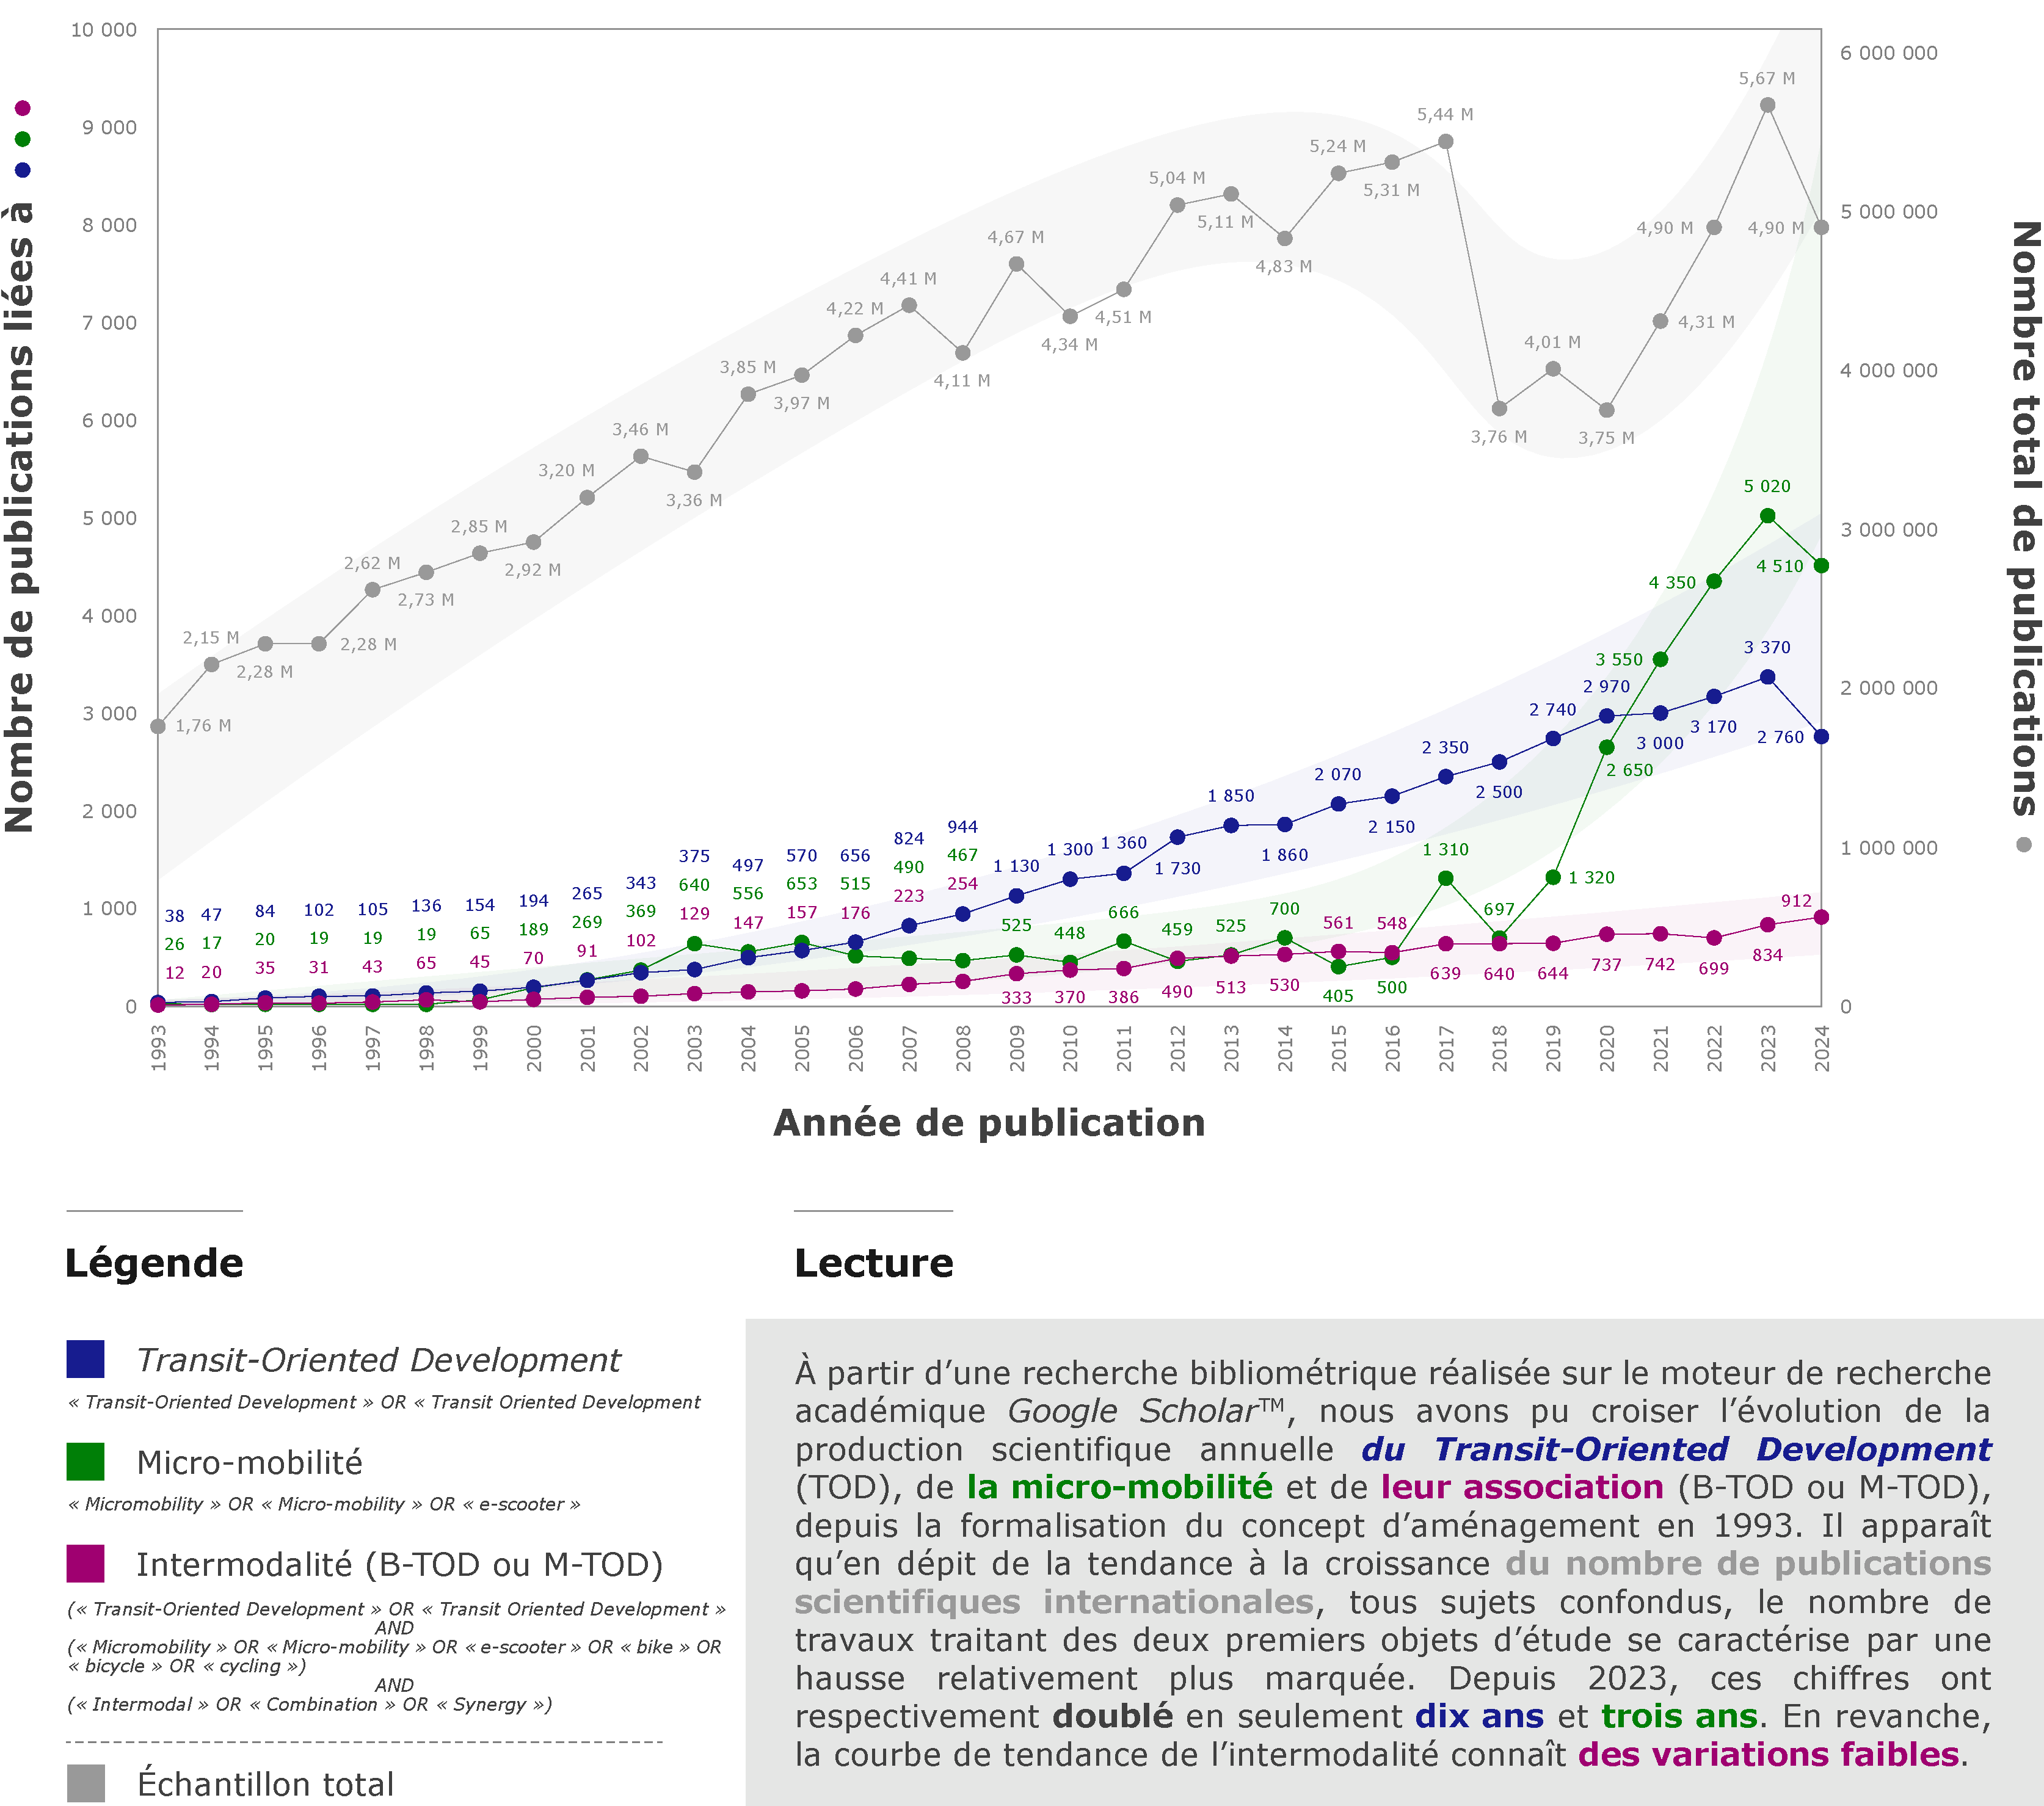
\includegraphics[width=1\columnwidth]{src/Figures/Chap-1/FR_Chronologie_publications_TOD_MIL.pdf}}
        \vspace{5pt}
        \begin{flushright}\scriptsize{
        Jeux de données~: données bibliométriques issues de \Marque{Google Scholar} et exportées le 2 février 2025
        \\
        Auteur~: \textcolor{blue}{Dylan Moinse (2025)}
      }\end{flushright}
    \end{figure}

    % M-TOD + Transition
L’une des évolutions récentes du \acrshort{TOD} explorées dans ce chapitre concerne l’intégration de la mobilité individuelle légère. Ces modes de déplacement complètent les infrastructures traditionnelles en offrant des solutions efficaces aux défis des \Guillemets{premiers et derniers kilomètres}. Toutefois, les connaissances sur cette forme d’intermodalité, en particulier sous l’angle de son articulation avec les formes urbaines, demeurent encore limitées. Ce constat est d’autant plus marqué pour les mobilités émergentes qui composent cette famille de modes, dont les interactions avec le \acrshort{TOD} restent largement inexplorées. Une simple recherche lexicale sur les thématiques du \acrshort{TOD} et de la micro-mobilité illustre combien ces sujets suscitent un intérêt croissant dans la recherche académique, comme l'atteste le \hyperref[fig-chap1:trends-google-scholar]{diagramme~\ref{fig-chap1:trends-google-scholar}} (page~\pageref{fig-chap1:trends-google-scholar}). Néanmoins, cette montée en puissance ne se traduit pas encore par une véritable synergie entre ces deux champs d’étude, qui restent peu représentés conjointement dans la littérature scientifique. Ce chapitre, qui pose le cadre théorique de notre recherche, se conclut ainsi par un constat~: celui d’un déficit de connaissances \textsl{a priori} sur un sujet redécouvert récemment dans le contexte du \acrshort{TOD}. Cette lacune est également mise en évidence par \textcolor{blue}{Wei} \textcolor{blue}{\textcite[90]{kang_university_2020}}\index{Kang, Wei|pagebf}\index{Aguiléra, Anne|pagebf}\index{Rallet, Alain|pagebf}, qui fait remarquer dans sa thèse de doctorat le faible nombre d’études consacrées à l’intermodalité entre les nouveaux services de mobilité, à savoir le \acrshort{VFF}, et les transports en commun. De même, la \acrshort{TEP} et la \acrshort{TEFF} n’ont été que marginalement étudiées, en dehors des problématiques liées à la traumatologie ou à l’accidentologie, alors même que leur potentiel intermodal est largement rapporté \textcolor{blue}{\autocite{richer_dossier_2021}}\index{Richer, Cyprien|pagebf}. Mener des études empiriques rigoureuses sur ces formes d’intermodalité apparaît comme une exigence pour mesurer et comprendre les comportements liés au \textsl{bike-and-ride} et au \textsl{scoot-and-ride}. \textcolor{blue}{\autocite[13]{bortoli_consequential_2020}}\index{Bortoli, Anne de|pagebf}\index{Christoforou, Zoi|pagebf}. Compte tenu de ce bilan, nous avons choisi d’engager un premier travail exploratoire sur ce que nous dénommons \acrshort{M-TOD}, en établissant un inventaire des travaux existants sur cette thématique, qui sera présenté dans le prochain chapitre.%%Rédigé%%

% ___________________________________________
     \newpage
     
% Valorisation scientifique
    \begin{tcolorbox}[colback=white!5!white,
                      colframe=blue!75!blue,
                      title=Valorisation scientifique
                      \\
                      Chapitre~1]
\Large{\textcolor{blue}{\textbf{Manifestations scientifiques~:}}}
    \\\\
\small{\textcolor{blue}{\textcite{moinse_transit-oriented_2021}}. Le Transit-Oriented Development, un urbanisme axé sur les transports en commun, intégrant les micro-mobilités émergentes. Une investigation sur les trottinettes personnelles en intermodalité, dans la région Hauts-de-France. \textsl{Rencontres TerriTrans - MoTAU}, Paris.
\\
\footnotesize{\url{https://hal.science/hal-03473391}} (\textbf{C-COM})}
    \\\\
\small{\textcolor{blue}{\textcite{moinse_modeurbain_2021}}. Le modèle urbain du Transit-Oriented Development revisité par les mobilités émergentes~? Une investigation sur le territoire de la région Hauts-de-France. \textsl{Rencontres Internationales en Urbanisme de l'APERAU}, Rabat.
\\
\footnotesize{\url{https://shs.hal.science/halshs-03507291}} (\textbf{C-COM})}
    \\\\
\small{\textcolor{blue}{\textcite{moinse_modeurbain_2020}}. Le modèle urbain du Transit-Oriented Development revisité par les micro-mobilités émergentes~? Une investigation sur le territoire de la région Hauts-de-France. \textsl{(Post-)Doctoriales AME 2020}, Le Croisic.
\\
\footnotesize{\url{https://shs.hal.science/halshs-03507482}} (\textbf{C-COM})}
    \\\\
\small{\textcolor{blue}{\textcite{moinse_etat_2020}}. État de l'art sur l'usage des trottinettes électriques en libre-service sans station. \textsl{Journées Transports \& Déplacements du Réseau Scientifique et Technique} (JTD RST). 
\\
\footnotesize{\url{https://shs.hal.science/halshs-03507375}} (\textbf{C-COM})}
    \\\\
\Large{\textcolor{blue}{\textbf{Vulgarisation scientifique~:}}}
    \\\\
\normalsize{\textcolor{blue}{\textcite{moinse_exploring_2023}}. \foreignlanguage{english}{\textsl{Exploring Val d'Europe's Urban Development in Marne-la-Vallée: A Guided Walking Tour of the TOD Project}}, Présentation de terrain, Paris
\\
\footnotesize{\url{https://shs.hal.science/halshs-04212064}}}
    \end{tcolorbox}

    % ___________________________________________
    % Sous-bibliographie
    \newpage
    \sectionheader{Sous-bibliographie du chapitre~1}
    \begingroup
    \renewcommand{\bibfont}{\scriptsize}
\printbibliography[segment=\therefsegment, heading=subbibintoc, title={Sous-bibliographie du chapitre~1}, label=chap1:bibliographie]
    \endgroup
    \end{refsegment}